\documentclass[twoside]{book}

% Packages required by doxygen
\usepackage{calc}
\usepackage{doxygen}
\usepackage{graphicx}
\usepackage[utf8]{inputenc}
\usepackage{makeidx}
\usepackage{multicol}
\usepackage{multirow}
\usepackage{textcomp}
\usepackage[table]{xcolor}

% Font selection
\usepackage[T1]{fontenc}
\usepackage{mathptmx}
\usepackage[scaled=.90]{helvet}
\usepackage{courier}
\usepackage{amssymb}
\usepackage{sectsty}
\renewcommand{\familydefault}{\sfdefault}
\allsectionsfont{%
  \fontseries{bc}\selectfont%
  \color{darkgray}%
}
\renewcommand{\DoxyLabelFont}{%
  \fontseries{bc}\selectfont%
  \color{darkgray}%
}

% Page & text layout
\usepackage{geometry}
\geometry{%
  a4paper,%
  top=2.5cm,%
  bottom=2.5cm,%
  left=2.5cm,%
  right=2.5cm%
}
\tolerance=750
\hfuzz=15pt
\hbadness=750
\setlength{\emergencystretch}{15pt}
\setlength{\parindent}{0cm}
\setlength{\parskip}{0.2cm}
\makeatletter
\renewcommand{\paragraph}{%
  \@startsection{paragraph}{4}{0ex}{-1.0ex}{1.0ex}{%
    \normalfont\normalsize\bfseries\SS@parafont%
  }%
}
\renewcommand{\subparagraph}{%
  \@startsection{subparagraph}{5}{0ex}{-1.0ex}{1.0ex}{%
    \normalfont\normalsize\bfseries\SS@subparafont%
  }%
}
\makeatother

% Headers & footers
\usepackage{fancyhdr}
\pagestyle{fancyplain}
\fancyhead[LE]{\fancyplain{}{\bfseries\thepage}}
\fancyhead[CE]{\fancyplain{}{}}
\fancyhead[RE]{\fancyplain{}{\bfseries\leftmark}}
\fancyhead[LO]{\fancyplain{}{\bfseries\rightmark}}
\fancyhead[CO]{\fancyplain{}{}}
\fancyhead[RO]{\fancyplain{}{\bfseries\thepage}}
\fancyfoot[LE]{\fancyplain{}{}}
\fancyfoot[CE]{\fancyplain{}{}}
\fancyfoot[RE]{\fancyplain{}{\bfseries\scriptsize Generated on Sat Aug 18 2018 22\-:39\-:34 for V\-L\-S\-I S\-A\-P\-D by Doxygen }}
\fancyfoot[LO]{\fancyplain{}{\bfseries\scriptsize Generated on Sat Aug 18 2018 22\-:39\-:34 for V\-L\-S\-I S\-A\-P\-D by Doxygen }}
\fancyfoot[CO]{\fancyplain{}{}}
\fancyfoot[RO]{\fancyplain{}{}}
\renewcommand{\footrulewidth}{0.4pt}
\renewcommand{\chaptermark}[1]{%
  \markboth{#1}{}%
}
\renewcommand{\sectionmark}[1]{%
  \markright{\thesection\ #1}%
}

% Indices & bibliography
\usepackage{natbib}
\usepackage[titles]{tocloft}
\setcounter{tocdepth}{3}
\setcounter{secnumdepth}{5}
\makeindex

% Hyperlinks (required, but should be loaded last)
\usepackage{ifpdf}
\ifpdf
  \usepackage[pdftex,pagebackref=true]{hyperref}
\else
  \usepackage[ps2pdf,pagebackref=true]{hyperref}
\fi
\hypersetup{%
  colorlinks=true,%
  linkcolor=blue,%
  citecolor=blue,%
  unicode%
}

% Custom commands
\newcommand{\clearemptydoublepage}{%
  \newpage{\pagestyle{empty}\cleardoublepage}%
}


%===== C O N T E N T S =====

\begin{document}

% Titlepage & ToC
\hypersetup{pageanchor=false}
\pagenumbering{roman}
\begin{titlepage}
\vspace*{7cm}
\begin{center}%
{\Large V\-L\-S\-I S\-A\-P\-D }\\
\vspace*{1cm}
{\large Generated by Doxygen 1.8.5}\\
\vspace*{0.5cm}
{\small Sat Aug 18 2018 22:39:34}\\
\end{center}
\end{titlepage}
\clearemptydoublepage
\tableofcontents
\clearemptydoublepage
\pagenumbering{arabic}
\hypersetup{pageanchor=true}

%--- Begin generated contents ---
\chapter{Presentation}
\label{index}\hypertarget{index}{}This documentation adresses two level of explanations \+:


\begin{DoxyItemize}
\item The {\bfseries A\+PI} description which explains how to use \mbox{\hyperlink{namespaceKite}{Kite}}, thoses parts as flagged as {\bfseries A\+PI}. 
\item The internal description which details how \mbox{\hyperlink{namespaceKite}{Kite}} do things. It\textquotesingle{}s mostly intended for myself to help me not to forget how I\textquotesingle{}ve done things when debug time will come... It may also be valuable to people who may want to use or patch \mbox{\hyperlink{namespaceKite}{Kite}} for their own purpose (my secret hope). 
\end{DoxyItemize}

Additionnal documents\+:
\begin{DoxyItemize}
\item \mbox{\hyperlink{group__grpSynthHierarchy}{Synthetic Hierarchy (A\+PI)}} 
\end{DoxyItemize}
\chapter{A\-G\-D\-S Format}
\label{agds}
\hypertarget{agds}{}
\hypertarget{agds_agdsPres}{}\section{Presentation}\label{agds_agdsPres}
The {\bfseries Ascii Graphic Database System (A\+G\+DS)} format is an ascii (text) version of the wellknown and industry standard G\+DS II binary format. This format hierarchicaly represents geometric shapes, labels and other layout informations (see \href{http://en.wikipedia.org/wiki/GDSII}{\tt http\+://en.\+wikipedia.\+org/wiki/\+G\+D\+S\+II} for more informations). ~\newline
The ascii format has several advantages versus binary format\+:
\begin{DoxyItemize}
\item human readable,
\item easy to edit manually or with dedicated tools,
\item easy to search or grep into,
\item easy to compare and understand differences between two files,
\item easy to convert.
\end{DoxyItemize}

The conversion from Ascii G\+DS to binary G\+DS and vice versa can be done with {\bfseries Owl\+Vision G\+D\+S\+II Viewer} available at \href{http://owlvision.org}{\tt http\+://owlvision.\+org}~\newline
Since it has been developped in java, it can be run on all platforms.\hypertarget{agds_agdsAutrhos}{}\subsection{Author}\label{agds_agdsAutrhos}
Damien Dupuis\+: damien.\+dupuis(at)lip6(.)fr\hypertarget{agds_agdsLimits}{}\subsection{Limitations}\label{agds_agdsLimits}
Currently the only supported shape in this driver is the rectangle.\hypertarget{agds_agdsDB}{}\section{Stand alone database structure}\label{agds_agdsDB}
The database conists in for simple objects \+:
\begin{DoxyItemize}
\item \hyperlink{class_a_g_d_s_1_1_library}{A\+G\+D\+S\+::\+Library} contains all A\+G\+DS library informations such as the name, the units used (user and physical) and the list of all Structures.
\item \hyperlink{class_a_g_d_s_1_1_structure}{A\+G\+D\+S\+::\+Structure} describes a G\+DS Structure with a name and a list of Elements.
\item \hyperlink{class_a_g_d_s_1_1_element}{A\+G\+D\+S\+::\+Element} is an abstract class from which derived the \hyperlink{class_a_g_d_s_1_1_rectangle}{A\+G\+D\+S\+::\+Rectangle}.
\item \hyperlink{class_a_g_d_s_1_1_rectangle}{A\+G\+D\+S\+::\+Rectangle} describes a rectangle element of a structure.
\end{DoxyItemize}\hypertarget{agds_agdsDriver}{}\subsection{Using the driver}\label{agds_agdsDriver}
To drive an A\+G\+DS file, user has to create one \hyperlink{class_a_g_d_s_1_1_library}{A\+G\+D\+S\+::\+Library} and add \hyperlink{class_a_g_d_s_1_1_structure}{A\+G\+D\+S\+::\+Structure} objects to it with the \hyperlink{class_a_g_d_s_1_1_library_a93d333a20154e0b688ff3ff213039171}{A\+G\+D\+S\+::\+Library\+::add\+Structure()} method. Each \hyperlink{class_a_g_d_s_1_1_structure}{A\+G\+D\+S\+::\+Structure} contains at least one \hyperlink{class_a_g_d_s_1_1_element}{A\+G\+D\+S\+::\+Element} added with \hyperlink{class_a_g_d_s_1_1_structure_a2dd203e6770f7d15d6f706867c919a60}{A\+G\+D\+S\+::\+Structure\+::add\+Element()} method.~\newline
All objects can be independently created as far as they are correctly added to their parent. ~\newline
Once the library is completely specified, simply call the \hyperlink{class_a_g_d_s_1_1_library_a33b9d989b84857f46034085664ff3fa2}{A\+G\+D\+S\+::\+Library\+::write\+To\+File()} method to drive the database to file.\hypertarget{agds_agdsExamples}{}\section{Examples}\label{agds_agdsExamples}
As said is the global presentation, V\+L\+SI S\+A\+PD project provides C++ libraries and Python modules for each supported format. In this section we present two simple code examples to drive a A\+G\+DS file using C++ or Python. These two examples drive the same file {\ttfamily transistor.\+agds\+:} 
\begin{DoxyCodeInclude}
HEADER 5;
BGNLIB;
  LASTMOD \{10-06-11  14:02:15\};
  LASTACC \{10-06-11  14:02:15\};
LIBNAME myTestLib.DB;
UNITS;
  USERUNITS 0.001;
  PHYSUNITS 1.000000e-09;

BGNSTR;
  CREATION \{10-06-11  14:02:15\};
  LASTMOD  \{10-06-11  14:02:15\};
STRNAME Transistor;

BOUNDARY;
LAYER 17;
DATATYPE 0;
XY 5;
  X: 305;   Y: 150;
  X: 305;   Y: 830;
  X: 365;   Y: 830;
  X: 365;   Y: 150;
  X: 305;   Y: 150;
ENDEL;

BOUNDARY;
LAYER 6;
DATATYPE 0;
XY 5;
  X: 130;   Y: 290;
  X: 130;   Y: 690;
  X: 540;   Y: 690;
  X: 540;   Y: 290;
  X: 130;   Y: 290;
ENDEL;

ENDSTR;
ENDLIB;
\end{DoxyCodeInclude}


 
\begin{DoxyImage}
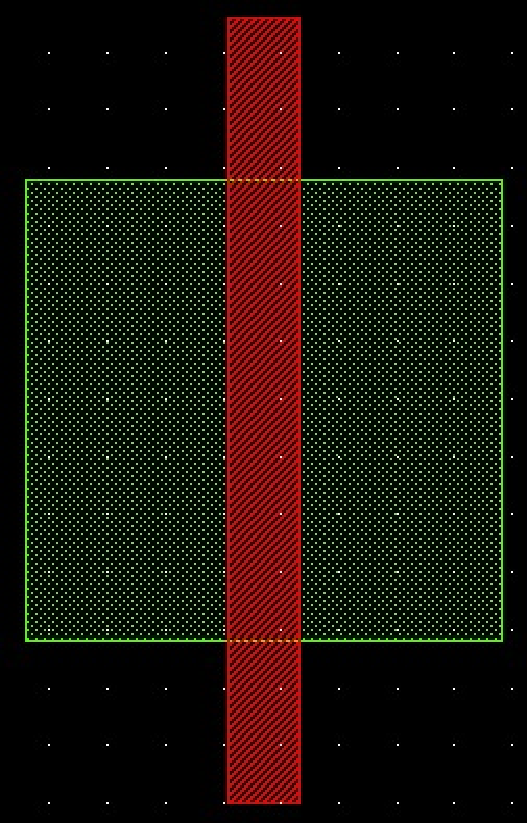
\includegraphics[width=.25\linewidth]{transistorCif}
\doxyfigcaption{A\+G\+DS example layout }
\end{DoxyImage}
\hypertarget{agds_agdsC}{}\subsection{C++}\label{agds_agdsC}
Here is the C++ code ({\ttfamily drive\+Agds.\+cpp}) used to generate the transistor.\+agds file. (Source is available in examples directory). 
\begin{DoxyCodeInclude}
\textcolor{preprocessor}{#include <string>}
\textcolor{keyword}{using namespace }\hyperlink{namespacestd}{std};

\textcolor{preprocessor}{#include "vlsisapd/agds/Library.h"}
\textcolor{preprocessor}{#include "vlsisapd/agds/Structure.h"}
\textcolor{preprocessor}{#include "vlsisapd/agds/Rectangle.h"}

\textcolor{keywordtype}{int} main(\textcolor{keywordtype}{int} argc, \textcolor{keywordtype}{char} * argv[]) \{
    \hyperlink{class_a_g_d_s_1_1_library}{AGDS::Library}* lib = \textcolor{keyword}{new} \hyperlink{class_a_g_d_s_1_1_library}{AGDS::Library}(\textcolor{keywordtype}{string}(\textcolor{stringliteral}{"myTestLib"}));

    lib->\hyperlink{class_a_g_d_s_1_1_library_a0d0e972bb142f892c462bb8d7f04a50b}{setUserUnits}(0.001);
    lib->\hyperlink{class_a_g_d_s_1_1_library_a938acb6eb8d14aade9dba7331c75ff0a}{setPhysUnits}(1.0E-9);

    \hyperlink{class_a_g_d_s_1_1_rectangle}{AGDS::Rectangle}* poly   = \textcolor{keyword}{new} \hyperlink{class_a_g_d_s_1_1_rectangle}{AGDS::Rectangle}( 17, 305, 150, 365, 830 );
    \hyperlink{class_a_g_d_s_1_1_rectangle}{AGDS::Rectangle}* active = \textcolor{keyword}{new} \hyperlink{class_a_g_d_s_1_1_rectangle}{AGDS::Rectangle}(  6, 130, 290, 540, 690 );

    \hyperlink{class_a_g_d_s_1_1_structure}{AGDS::Structure}* str = \textcolor{keyword}{new} \hyperlink{class_a_g_d_s_1_1_structure}{AGDS::Structure}(\textcolor{stringliteral}{"Transistor"});

    str->\hyperlink{class_a_g_d_s_1_1_structure_a2dd203e6770f7d15d6f706867c919a60}{addElement}(poly);
    str->\hyperlink{class_a_g_d_s_1_1_structure_a2dd203e6770f7d15d6f706867c919a60}{addElement}(active);

    lib->\hyperlink{class_a_g_d_s_1_1_library_a93d333a20154e0b688ff3ff213039171}{addStructure}(str);

    lib->\hyperlink{class_a_g_d_s_1_1_library_a33b9d989b84857f46034085664ff3fa2}{writeToFile}(\textcolor{stringliteral}{"./transistor.agds"});
    
    \textcolor{keywordflow}{return} 0;
\}

\end{DoxyCodeInclude}


\begin{DoxyNote}{Note}
In order to compile this code, a C\+Make\+Lists.\+txt file is provided. User must set the \$\+V\+L\+S\+I\+S\+A\+P\+D\+\_\+\+T\+OP variable before running these commands in the directory containing the C\+Make\+Lists.\+txt file\+: 
\begin{DoxyCode}
%> mkdir build; cd build
%> cmake ..
%> make
\end{DoxyCode}

\end{DoxyNote}
\hypertarget{agds_agdsPython}{}\subsection{Python}\label{agds_agdsPython}
Here is the Python code ({\ttfamily drive\+Agds.\+py}) used to generate the transistor.\+agds file. (Source is available in examples directory). 
\begin{DoxyCodeInclude}
\textcolor{keyword}{import} AGDS
lib = \hyperlink{class_a_g_d_s_1_1_library}{AGDS.Library}(\textcolor{stringliteral}{"myTestLib"})
lib.setUserUnits(0.001)
lib.setPhysUnits(1.0e-9)

active = \hyperlink{class_a_g_d_s_1_1_rectangle}{AGDS.Rectangle}( 6, 120, 290, 540, 690) \textcolor{comment}{# layer  6 corresponds to active}
poly   = \hyperlink{class_a_g_d_s_1_1_rectangle}{AGDS.Rectangle}(17, 305, 150, 365, 830) \textcolor{comment}{# layer 17 corresponds to polysilicium}

str = \hyperlink{class_a_g_d_s_1_1_structure}{AGDS.Structure}(\textcolor{stringliteral}{"Transistor"})
str.addElement(active)
str.addElement(poly)

lib.addStructure(str)
lib.writeToFile(\textcolor{stringliteral}{"./transistor.agds"})
\end{DoxyCodeInclude}


\begin{DoxyNote}{Note}
In order to run the {\ttfamily drive\+Agds.\+py} script, user must ensure that \$\+P\+Y\+T\+H\+O\+N\+P\+A\+TH variable points to the directory containing A\+G\+D\+S.\+so module. 
\end{DoxyNote}

\chapter{C\-I\-F Format}
\label{cif}
\hypertarget{cif}{}
\hypertarget{cif_cifPres}{}\section{Presentation}\label{cif_cifPres}
The {\bfseries Caltech Intermediate Format (C\+IF)} consists in a limited set of graphic primitives used to describe the shapes on each layer of an integrated circuit (see \href{http://en.wikipedia.org/wiki/Caltech_Intermediate_Form}{\tt http\+://en.\+wikipedia.\+org/wiki/\+Caltech\+\_\+\+Intermediate\+\_\+\+Form} for more informations). ~\newline
 \hypertarget{cif_cifAutrhos}{}\subsection{Author}\label{cif_cifAutrhos}
Damien Dupuis\+: damien.\+dupuis(at)lip6(.)fr\hypertarget{cif_cifLimits}{}\subsection{Limitations}\label{cif_cifLimits}
Although the C\+IF format allows hierarchical description and supports several shapes, in this driver, we do not use hierarchy and only use Polygons.\hypertarget{cif_cifDB}{}\section{Stand alone database structure}\label{cif_cifDB}
The database consists in two simple objects \+:
\begin{DoxyItemize}
\item \hyperlink{class_c_i_f_1_1_circuit}{C\+I\+F\+::\+Circuit} contains all C\+IF circuit informations such as the name, the unit used, the scale and the list of all Polygons.
\item \hyperlink{class_c_i_f_1_1_polygon}{C\+I\+F\+::\+Polygon} describes a Polygon (a set of points).
\end{DoxyItemize}\hypertarget{cif_cifDriver}{}\subsection{Using the driver}\label{cif_cifDriver}
To drive a C\+IF file, user has to create one \hyperlink{class_c_i_f_1_1_circuit}{C\+I\+F\+::\+Circuit} and as many \hyperlink{class_c_i_f_1_1_polygon}{C\+I\+F\+::\+Polygon} as the number of shapes of the layout. The \hyperlink{class_c_i_f_1_1_polygon}{C\+I\+F\+::\+Polygon} objects can be created independently from for the \hyperlink{class_c_i_f_1_1_circuit}{C\+I\+F\+::\+Circuit} but must be finally added to the \hyperlink{class_c_i_f_1_1_circuit}{C\+I\+F\+::\+Circuit} using \hyperlink{class_c_i_f_1_1_circuit_a5b37e86206e2a128ba6db4987dc09a39}{C\+I\+F\+::\+Circuit\+::add\+Polygon()}.~\newline
Once the \hyperlink{class_c_i_f_1_1_circuit}{C\+I\+F\+::\+Circuit} is complete, simply call the \hyperlink{class_c_i_f_1_1_circuit_a90c823b70c4984f302c19ceca604d101}{C\+I\+F\+::\+Circuit\+::write\+To\+File()} method to drive the database to file.\hypertarget{cif_cifExamples}{}\section{Examples}\label{cif_cifExamples}
As said is the global presentation, V\+L\+SI S\+A\+PD project provides C++ libraries and Python modules for each supported format. In this section we present two simple code examples to drive a C\+IF file using C++ or Python. These two examples drive the same file {\ttfamily transistor.\+cif\+:} 
\begin{DoxyCodeInclude}
(CIF file written on 11-Jun-2010  13:49:44 by VLSISAPD\_CIF\_DRIVER);
(Units: micro  -  UU/DB Scale: 0.001);
DS 1 1 1;
9 Transistor;
L 6; P 130,290 540,290 540,690 130,690;
L 17; P 305,150 365,150 365,830 305,830;
DF;
C 1;
E
\end{DoxyCodeInclude}


 
\begin{DoxyImage}
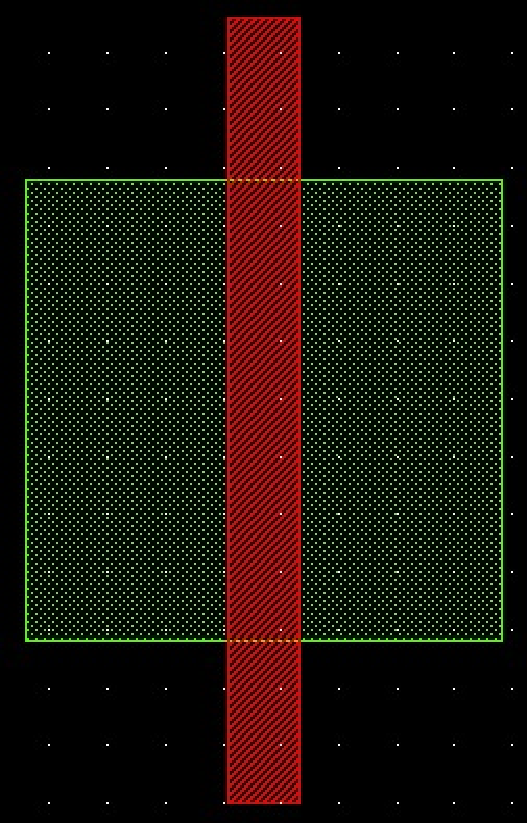
\includegraphics[width=.25\linewidth]{transistorCif}
\doxyfigcaption{C\+IF example layout }
\end{DoxyImage}
\hypertarget{cif_cifC}{}\subsection{C++}\label{cif_cifC}
Here is the C++ code ({\ttfamily drive\+Cif.\+cpp}) used to generate the transistor.\+cif file. (Source is available in examples directory). 
\begin{DoxyCodeInclude}
\textcolor{preprocessor}{#include <string>}
\textcolor{keyword}{using namespace }\hyperlink{namespacestd}{std};

\textcolor{preprocessor}{#include "vlsisapd/cif/Circuit.h"}
\textcolor{preprocessor}{#include "vlsisapd/cif/Polygon.h"}

\textcolor{keywordtype}{int} main(\textcolor{keywordtype}{int} argc, \textcolor{keywordtype}{char} * argv[]) \{
    \hyperlink{class_c_i_f_1_1_circuit}{CIF::Circuit}* circuit = \textcolor{keyword}{new} \hyperlink{class_c_i_f_1_1_circuit}{CIF::Circuit}(\textcolor{keywordtype}{string}(\textcolor{stringliteral}{"Transistor"}), \textcolor{keywordtype}{string}(\textcolor{stringliteral}{"micro"}),
       0.001);

    \textcolor{comment}{// Layer #6 corresponds to active}
    \hyperlink{class_c_i_f_1_1_polygon}{CIF::Polygon}* poly = \textcolor{keyword}{new} \hyperlink{class_c_i_f_1_1_polygon}{CIF::Polygon}(6);
    poly->\hyperlink{class_c_i_f_1_1_polygon_ab3047469780327f18539907e1303ea15}{addPoint}(130, 290);
    poly->\hyperlink{class_c_i_f_1_1_polygon_ab3047469780327f18539907e1303ea15}{addPoint}(540, 290);
    poly->\hyperlink{class_c_i_f_1_1_polygon_ab3047469780327f18539907e1303ea15}{addPoint}(540, 690);
    poly->\hyperlink{class_c_i_f_1_1_polygon_ab3047469780327f18539907e1303ea15}{addPoint}(130, 690);
    circuit->\hyperlink{class_c_i_f_1_1_circuit_a5b37e86206e2a128ba6db4987dc09a39}{addPolygon}(poly);

    \textcolor{comment}{// Layer #17 corresponds to polysilicium}
    poly = \textcolor{keyword}{new} \hyperlink{class_c_i_f_1_1_polygon}{CIF::Polygon}(17);
    poly->\hyperlink{class_c_i_f_1_1_polygon_ab3047469780327f18539907e1303ea15}{addPoint}(305, 150);
    poly->\hyperlink{class_c_i_f_1_1_polygon_ab3047469780327f18539907e1303ea15}{addPoint}(365, 150);
    poly->\hyperlink{class_c_i_f_1_1_polygon_ab3047469780327f18539907e1303ea15}{addPoint}(365, 830);
    poly->\hyperlink{class_c_i_f_1_1_polygon_ab3047469780327f18539907e1303ea15}{addPoint}(305, 830);
    circuit->\hyperlink{class_c_i_f_1_1_circuit_a5b37e86206e2a128ba6db4987dc09a39}{addPolygon}(poly);

    circuit->\hyperlink{class_c_i_f_1_1_circuit_a90c823b70c4984f302c19ceca604d101}{writeToFile}(\textcolor{stringliteral}{"./transistor.cif"});
    
    \textcolor{keywordflow}{return} 0;
\}

\end{DoxyCodeInclude}


\begin{DoxyNote}{Note}
In order to compile this code, a C\+Make\+Lists.\+txt file is provided. User must set the \$\+V\+L\+S\+I\+S\+A\+P\+D\+\_\+\+T\+OP variable before running these commands in the directory containing the C\+Make\+Lists.\+txt file\+: 
\begin{DoxyCode}
%> mkdir build; cd build
%> cmake ..
%> make
\end{DoxyCode}

\end{DoxyNote}
\hypertarget{cif_cifPython}{}\subsection{Python}\label{cif_cifPython}
Here is the Python code ({\ttfamily drive\+Cif.\+py}) used to generate the transistor.\+cif file. (Source is available in examples directory). 
\begin{DoxyCodeInclude}
\textcolor{keyword}{import} CIF
circuit = \hyperlink{class_c_i_f_1_1_circuit}{CIF.Circuit}(\textcolor{stringliteral}{"Transistor"}, \textcolor{stringliteral}{"micro"}, 0.001)
poly1 = \hyperlink{class_c_i_f_1_1_polygon}{CIF.Polygon}(6)
poly1.addPoint(130, 290)
poly1.addPoint(540, 290)
poly1.addPoint(540, 690)
poly1.addPoint(130, 690)
circuit.addPolygon(poly1)
    
poly2 = \hyperlink{class_c_i_f_1_1_polygon}{CIF.Polygon}(17)
poly2.addPoint(305, 150);
poly2.addPoint(365, 150);
poly2.addPoint(365, 830);
poly2.addPoint(305, 830);
circuit.addPolygon(poly2)

circuit.writeToFile(\textcolor{stringliteral}{"./transistor.cif"})
\end{DoxyCodeInclude}


\begin{DoxyNote}{Note}
In order to run the {\ttfamily drive\+Cif.\+py} script, user must ensure that \$\+P\+Y\+T\+H\+O\+N\+P\+A\+TH variable points to the directory containing C\+I\+F.\+so module. 
\end{DoxyNote}

\chapter{Links \& Contacts}
\label{contact}
\hypertarget{contact}{}
V\+L\+SI S\+A\+PD project is developped at the {\itshape Pierre \& Marie Curie University} in {\itshape Paris}, {\itshape France} (\href{http://www.upmc.fr}{\tt http\+://www.\+upmc.\+fr}) at the L\+I\+P6 laboratory (\href{http://www.lip6.fr}{\tt http\+://www.\+lip6.\+fr}).~\newline
~\newline
 It is used by\+:
\begin{DoxyItemize}
\item Coriolis 2 Project\+: \href{http://www-soc.lip6.fr/recherche/cian/coriolis-2/}{\tt http\+://www-\/soc.\+lip6.\+fr/recherche/cian/coriolis-\/2/}
\item Chams Project\+: \href{http://www-soc.lip6.fr/recherche/cian/chams/}{\tt http\+://www-\/soc.\+lip6.\+fr/recherche/cian/chams/}~\newline
~\newline
 For any information you can contact the author of a parser / driver (if available on corresponding page) or Damien Dupuis\+: damien.\+dupuis(at)lip6(.)fr founder of the project. 
\end{DoxyItemize}
\chapter{D\-T\-R Format}
\label{dtr}
\hypertarget{dtr}{}
\hypertarget{dtr_dtrPres}{}\section{Presentation}\label{dtr_dtrPres}
The {\bfseries Design Technology Rules (D\-T\-R)} format was developped as a part of the Chams Project (\href{http://www-soc.lip6.fr/recherche/cian/chams/}{\tt http\-://www-\/soc.\-lip6.\-fr/recherche/cian/chams/}). It aims at offering a generic description of layout design rules for C\-M\-O\-S technologies.\par
 \hypertarget{dtr_dtrAutrhos}{}\subsection{Author}\label{dtr_dtrAutrhos}
Damien Dupuis\-: damien.\-dupuis(at)lip6(.)fr\hypertarget{dtr_dtrLimits}{}\subsection{Limitations}\label{dtr_dtrLimits}
Only simple rules are supported at the moment. For example the minimum width of a metal layer has only one value, although it should depends on the length of the wire drawned.\hypertarget{dtr_dtrDB}{}\section{Stand alone database structure}\label{dtr_dtrDB}
The database contains four object \-:
\begin{DoxyItemize}
\item \hyperlink{class_d_t_r_1_1_techno}{D\-T\-R\-::\-Techno} contains generic informations such as the name of the technology and the unit used, and the list of all technologic rules.
\item \hyperlink{class_d_t_r_1_1_rule}{D\-T\-R\-::\-Rule} \& \hyperlink{class_d_t_r_1_1_a_rule}{D\-T\-R\-::\-A\-Rule} respectively describe a symmetrical and an asymmetrical rule.
\end{DoxyItemize}

The library also use the \hyperlink{class_d_t_r_1_1_d_t_r_exception}{D\-T\-R\-::\-D\-T\-R\-Exception} class to throw excptions.\hypertarget{dtr_dtrParser}{}\subsection{Using the parser}\label{dtr_dtrParser}
Simply load a technology with static function \hyperlink{class_d_t_r_1_1_techno_acf863c2bdb7f1aacc4422c8155c60d17}{D\-T\-R\-::\-Techno\-::read\-From\-File()} and then get rules (\hyperlink{class_d_t_r_1_1_techno_a4d56a05b47bd6c51e4e18120f49b584b}{D\-T\-R\-::\-Techno\-::get\-Rule()}) or directly values (\hyperlink{class_d_t_r_1_1_techno_ac08e2e60dd16750551221ca908001057}{D\-T\-R\-::\-Techno\-::get\-Value()}).\hypertarget{dtr_dtrDriver}{}\subsection{Using the driver}\label{dtr_dtrDriver}
Using the driver is very simple, user has to create a \hyperlink{class_d_t_r_1_1_techno}{D\-T\-R\-::\-Techno} object and simply add \hyperlink{class_d_t_r_1_1_rule}{D\-T\-R\-::\-Rule} or \hyperlink{class_d_t_r_1_1_a_rule}{D\-T\-R\-::\-A\-Rule} to it. The adding methods return the newly created Rule so user can set the rule type (\hyperlink{class_d_t_r_1_1_rule_a3568407d7a7890c39b8c9acc1e608535}{D\-T\-R\-::\-Rule\-::set\-Type()}) if necessary. Finally use the \hyperlink{class_d_t_r_1_1_techno_a26b05539dd3345963b8708788b82e2cb}{D\-T\-R\-::\-Techno\-::write\-To\-File()} method to dump the database to file.\hypertarget{dtr_dtrExamples}{}\section{Examples}\label{dtr_dtrExamples}
As said is the global presentation, V\-L\-S\-I S\-A\-P\-D project provides C++ libraries and Python modules for each supported format. In this section we present simple code examples to parse and drive a D\-T\-R file using C++ or Python. The D\-T\-R file considered is the same for all examples\-: {\ttfamily example.\-dtr.\-xml} 
\begin{DoxyCodeInclude}
<technology name=\textcolor{stringliteral}{"example"} unit=\textcolor{stringliteral}{"micro"} version=\textcolor{stringliteral}{"rev.A"}>
   <physical\_rules>
     <!-- transistor -->
     <rule  name=\textcolor{stringliteral}{"transistorMinL"}                                         value=\textcolor{stringliteral}{"0.10"}   ref=\textcolor{stringliteral}{"ref1"}/> 
     <rule  name=\textcolor{stringliteral}{"transistorMinW"}                                         value=\textcolor{stringliteral}{"0.20"}   ref=\textcolor{stringliteral}{"ref2"}/>

     <!-- minWidth -->
     <rule  name=\textcolor{stringliteral}{"minWidth"}           layer=\textcolor{stringliteral}{"metal1"}                      value=\textcolor{stringliteral}{"0.15"}   ref=\textcolor{stringliteral}{"ref3"}/>

     <!-- minSpacing -->
     <rule  name=\textcolor{stringliteral}{"minSpacing"}         layer=\textcolor{stringliteral}{"metal1"}                      value=\textcolor{stringliteral}{"0.20"}   ref=\textcolor{stringliteral}{"ref4"}/>
     <rule  name=\textcolor{stringliteral}{"minSpacing"}         layer1=\textcolor{stringliteral}{"active"}   layer2=\textcolor{stringliteral}{"poly"}     value=\textcolor{stringliteral}{"0.10"}   ref=\textcolor{stringliteral}{"ref5"}/>

     <!-- minExtension -->
     <arule name=\textcolor{stringliteral}{"minExtension"}       layer1=\textcolor{stringliteral}{"poly"}     layer2=\textcolor{stringliteral}{"active"}   value=\textcolor{stringliteral}{"0.20"}   ref=\textcolor{stringliteral}{"ref6"}/>

     <!-- minArea -->
     <rule  name=\textcolor{stringliteral}{"minArea"}            type=\textcolor{stringliteral}{"area"}       layer=\textcolor{stringliteral}{"metal1"}    value=\textcolor{stringliteral}{"0.100"}  ref=\textcolor{stringliteral}{"ref7"}/>
  </physical\_rules>
</technology>

\end{DoxyCodeInclude}


All source codes are available in the {\ttfamily examples} directory.\hypertarget{dtr_dtrC}{}\subsection{C++}\label{dtr_dtrC}
\hypertarget{dtr_dtrParseC}{}\subsubsection{Parser}\label{dtr_dtrParseC}
The following code ({\ttfamily parse\-Dtr.\-cpp}) is an example of how to parse a D\-T\-R file using C++ library. 
\begin{DoxyCodeInclude}
\textcolor{preprocessor}{#include <iostream>}
\textcolor{preprocessor}{#include <string>}
\textcolor{keyword}{using namespace }std;

\textcolor{preprocessor}{#include "vlsisapd/dtr/Techno.h"}

\textcolor{keywordtype}{int} main(\textcolor{keywordtype}{int} argc, \textcolor{keywordtype}{char} * argv[]) \{
    \hyperlink{class_d_t_r_1_1_techno}{DTR::Techno}* techno = \hyperlink{class_d_t_r_1_1_techno_acf863c2bdb7f1aacc4422c8155c60d17}{DTR::Techno::readFromFile}(\textcolor{stringliteral}{"./example.dtr.xml"}
      );

    cerr << \textcolor{stringliteral}{"+-----------------------------+"} << endl
         << \textcolor{stringliteral}{"| technology:      "} << techno->\hyperlink{class_d_t_r_1_1_techno_aef436e6e20d1dbf2eb78b089ca9d0794}{getName}()    <<   \textcolor{stringliteral}{"    |"}   << endl
         << \textcolor{stringliteral}{"| units:           "} << techno->\hyperlink{class_d_t_r_1_1_techno_a4a8ae82fc3348771d0b53d9a3b11652d}{getUnit}()    << \textcolor{stringliteral}{"      |"} << endl
         << \textcolor{stringliteral}{"| version:         "} << techno->getVersion() << \textcolor{stringliteral}{"      |"} << endl
         << \textcolor{stringliteral}{"+-----------------------------+"} << endl << endl;

    cerr << \textcolor{stringliteral}{"transistorMinL                = "} << techno->\hyperlink{class_d_t_r_1_1_techno_ac08e2e60dd16750551221ca908001057}{getValue}(\textcolor{stringliteral}{"transistorMinL"}) << endl
         << \textcolor{stringliteral}{"transistorMinW                = "} << techno->\hyperlink{class_d_t_r_1_1_techno_ad5ef5b8e444ab7a86a2e3bff7762c956}{getValueAsString}(\textcolor{stringliteral}{"transistorMinW"}
      ) << endl
         << \textcolor{stringliteral}{"minWidth of metal1            = "} << techno->\hyperlink{class_d_t_r_1_1_techno_ac08e2e60dd16750551221ca908001057}{getValue}(\textcolor{stringliteral}{"minWidth"}, \textcolor{stringliteral}{"metal1"}) << endl
         << \textcolor{stringliteral}{"minSpacing of metal1          = "} << techno->\hyperlink{class_d_t_r_1_1_techno_ac08e2e60dd16750551221ca908001057}{getValue}(\textcolor{stringliteral}{"minWidth"}, \textcolor{stringliteral}{"metal1"}) << endl
         << \textcolor{stringliteral}{"minSpacing of active vs poly  = "} << techno->\hyperlink{class_d_t_r_1_1_techno_ac08e2e60dd16750551221ca908001057}{getValue}(\textcolor{stringliteral}{"minSpacing"}, \textcolor{stringliteral}{"active"}, \textcolor{stringliteral}{"poly"}) 
      << endl
         << \textcolor{stringliteral}{"minExtension active over poly = "} << techno->\hyperlink{class_d_t_r_1_1_techno_ac08e2e60dd16750551221ca908001057}{getValue}(\textcolor{stringliteral}{"minExtension"}, \textcolor{stringliteral}{"poly"}, \textcolor{stringliteral}{"active"}
      ) << endl
         << \textcolor{stringliteral}{"minArea of metal1             = "} << techno->\hyperlink{class_d_t_r_1_1_techno_ac08e2e60dd16750551221ca908001057}{getValue}(\textcolor{stringliteral}{"minArea"}, \textcolor{stringliteral}{"metal1"}) << endl;

    \textcolor{keywordflow}{return} 0;
\}

\end{DoxyCodeInclude}
\hypertarget{dtr_dtrDriveC}{}\subsubsection{Driver}\label{dtr_dtrDriveC}
This C++ code ({\ttfamily drive\-Dtr.\-cpp}) generates a out.\-dtr.\-xml file equivalent to the previous example.\-dtr.\-xml. 
\begin{DoxyCodeInclude}
\textcolor{preprocessor}{#include <string>}
\textcolor{keyword}{using namespace }std;

\textcolor{preprocessor}{#include "vlsisapd/dtr/Techno.h"}
\textcolor{preprocessor}{#include "vlsisapd/dtr/Rules.h"}

\textcolor{keywordtype}{int} main(\textcolor{keywordtype}{int} argc, \textcolor{keywordtype}{char} * argv[]) \{
    \hyperlink{class_d_t_r_1_1_techno}{DTR::Techno}* techno = \textcolor{keyword}{new} \hyperlink{class_d_t_r_1_1_techno}{DTR::Techno}(\textcolor{stringliteral}{"MyTech"}, \textcolor{stringliteral}{"micro"}, \textcolor{stringliteral}{"rev.A"});

    techno->\hyperlink{class_d_t_r_1_1_techno_afa2c8412c365c950649b9f81661ecafd}{addRule} (\textcolor{stringliteral}{"transistorMinL"}, 0.1 , \textcolor{stringliteral}{"ref1"});
    techno->\hyperlink{class_d_t_r_1_1_techno_afa2c8412c365c950649b9f81661ecafd}{addRule} (\textcolor{stringliteral}{"transistorMinW"}, 0.2 , \textcolor{stringliteral}{"ref2"});
    techno->\hyperlink{class_d_t_r_1_1_techno_afa2c8412c365c950649b9f81661ecafd}{addRule} (\textcolor{stringliteral}{"minWidth"}      , 0.15, \textcolor{stringliteral}{"ref3"}, \textcolor{stringliteral}{"metal1"});
    techno->\hyperlink{class_d_t_r_1_1_techno_afa2c8412c365c950649b9f81661ecafd}{addRule} (\textcolor{stringliteral}{"minSpacing"}    , 0.2 , \textcolor{stringliteral}{"ref4"}, \textcolor{stringliteral}{"metal1"});
    techno->\hyperlink{class_d_t_r_1_1_techno_afa2c8412c365c950649b9f81661ecafd}{addRule} (\textcolor{stringliteral}{"minSpacing"}    , 0.1 , \textcolor{stringliteral}{"ref5"}, \textcolor{stringliteral}{"active"}, \textcolor{stringliteral}{"poly"});
    techno->\hyperlink{class_d_t_r_1_1_techno_a5f5a790974fe7d3b1c6f1b698ef0a818}{addARule}(\textcolor{stringliteral}{"minExtension"}  , 0.2 , \textcolor{stringliteral}{"ref6"}, \textcolor{stringliteral}{"poly"}  , \textcolor{stringliteral}{"active"});
    
    \hyperlink{class_d_t_r_1_1_rule}{DTR::Rule}* rule = techno->\hyperlink{class_d_t_r_1_1_techno_afa2c8412c365c950649b9f81661ecafd}{addRule}(\textcolor{stringliteral}{"minArea"}, 0.1, \textcolor{stringliteral}{"ref7"}, \textcolor{stringliteral}{"metal1"});
    rule->\hyperlink{class_d_t_r_1_1_rule_a3568407d7a7890c39b8c9acc1e608535}{setType}(\textcolor{stringliteral}{"area"});

    techno->\hyperlink{class_d_t_r_1_1_techno_a26b05539dd3345963b8708788b82e2cb}{writeToFile}(\textcolor{stringliteral}{"./out.dtr.xml"});
    
    \textcolor{keywordflow}{return} 0;
\}

\end{DoxyCodeInclude}


\begin{DoxyNote}{Note}
In order to compile these codes, a C\-Make\-Lists.\-txt file is provided. User must set the \$\-V\-L\-S\-I\-S\-A\-P\-D\-\_\-\-T\-O\-P variable before running these commands in the directory containing the C\-Make\-Lists.\-txt file\-: 
\begin{DoxyCode}
%> mkdir build; cd build
%> cmake ..
%> make
\end{DoxyCode}

\end{DoxyNote}
\hypertarget{dtr_dtrPython}{}\subsection{Python}\label{dtr_dtrPython}
\hypertarget{dtr_dtrParsePython}{}\subsubsection{Parser}\label{dtr_dtrParsePython}
The following python script ({\ttfamily parse\-Dtr.\-py}) is an example of how to parse a D\-T\-R file using python module. 
\begin{DoxyCodeInclude}
1 \textcolor{keyword}{from} DTR \textcolor{keyword}{import} *
2 \textcolor{keyword}{from} decimal \textcolor{keyword}{import} Decimal
3 
4 techno = Techno.readFromFile(\textcolor{stringliteral}{"./example.dtr.xml"})
5 
6 \textcolor{keywordflow}{print} \textcolor{stringliteral}{"+-----------------------------+"}
7 \textcolor{keywordflow}{print} \textcolor{stringliteral}{"| technology:      "}+techno.get)   +  \textcolor{stringliteral}{"    |"}
8 \textcolor{keywordflow}{print} \textcolor{stringliteral}{"| units:           "}+techno.getUnit()   +\textcolor{stringliteral}{"      |"}
9 \textcolor{keywordflow}{print} \textcolor{stringliteral}{"| version:         "}+techno.getVersion()+\textcolor{stringliteral}{"      |"}
10 \textcolor{keywordflow}{print} \textcolor{stringliteral}{"+-----------------------------+\(\backslash\)n\(\backslash\)n"}
11 
12 \textcolor{keywordflow}{print} \textcolor{stringliteral}{"transistorMinL                = %s"}%techno.getValue(\textcolor{stringliteral}{"transistorMinL"})
13 \textcolor{keywordflow}{print} \textcolor{stringliteral}{"transistorMinW                = %s"}%Decimal(techno.getValueAsString(\textcolor{stringliteral}{"transistorMinW"}))
14 \textcolor{keywordflow}{print} \textcolor{stringliteral}{"minWidth of metal1            = %s"}%techno.getValue(\textcolor{stringliteral}{"minWidth"}, \textcolor{stringliteral}{"metal1"})
15 \textcolor{keywordflow}{print} \textcolor{stringliteral}{"minSpacing of metal1          = %s"}%techno.getValue(\textcolor{stringliteral}{"minWidth"}, \textcolor{stringliteral}{"metal1"})
16 \textcolor{keywordflow}{print} \textcolor{stringliteral}{"minSpacing of active vs poly  = %s"}%techno.getValue(\textcolor{stringliteral}{"minSpacing"}, \textcolor{stringliteral}{"active"}, \textcolor{stringliteral}{"poly"})
17 \textcolor{keywordflow}{print} \textcolor{stringliteral}{"minExtension active over poly = %s"}%techno.getValue(\textcolor{stringliteral}{"minExtension"}, \textcolor{stringliteral}{"poly"}, \textcolor{stringliteral}{"active"})
18 \textcolor{keywordflow}{print} \textcolor{stringliteral}{"minArea of metal1             = %s"}%techno.getValue(\textcolor{stringliteral}{"minArea"}, \textcolor{stringliteral}{"metal1"})
19 
20 \textcolor{comment}{# an example of why it is important to use Decimal in python:}
21 \textcolor{keywordflow}{print} techno.getValue(\textcolor{stringliteral}{"minArea"}, \textcolor{stringliteral}{"metal1"})*3-0.3 \textcolor{comment}{# returns 5.55111512313e-17}
22 \textcolor{keywordflow}{print} Decimal(techno.getValueAsString(\textcolor{stringliteral}{"minArea"}, \textcolor{stringliteral}{"metal1"}))*3-Decimal(\textcolor{stringliteral}{'0.3'}) \textcolor{comment}{# returns 0.000}
\end{DoxyCodeInclude}
\hypertarget{dtr_dtrDrivePython}{}\subsubsection{Driver}\label{dtr_dtrDrivePython}
This python script ({\ttfamily drive\-Dtr.\-py}) generates a out.\-dtr.\-xml file equivalent to the previous example.\-dtr.\-xml. 
\begin{DoxyCodeInclude}
1 \textcolor{keyword}{from} DTR \textcolor{keyword}{import} *
2 
3 techno = Techno(\textcolor{stringliteral}{"myTech"}, \textcolor{stringliteral}{"micro"}, \textcolor{stringliteral}{"rev.A"})
4 
5 techno.addRule (\textcolor{stringliteral}{"transistorMinL"}, 0.1 , \textcolor{stringliteral}{"ref1"})
6 techno.addRule (\textcolor{stringliteral}{"transistorMinW"}, 0.2 , \textcolor{stringliteral}{"ref2"})
7 techno.addRule (\textcolor{stringliteral}{"minWidth"}      , 0.15, \textcolor{stringliteral}{"ref3"}, \textcolor{stringliteral}{"metal1"})
8 techno.addRule (\textcolor{stringliteral}{"minSpacing"}    , 0.2 , \textcolor{stringliteral}{"ref4"}, \textcolor{stringliteral}{"metal1"})
9 techno.addRule (\textcolor{stringliteral}{"minSpacing"}    , 0.1 , \textcolor{stringliteral}{"ref5"}, \textcolor{stringliteral}{"active"}, \textcolor{stringliteral}{"poly"})
10 techno.addARule(\textcolor{stringliteral}{"minExtension"}  , 0.2 , \textcolor{stringliteral}{"ref6"}, \textcolor{stringliteral}{"poly"}, \textcolor{stringliteral}{"active"})
11 
12 rule = techno.addRule(\textcolor{stringliteral}{"minArea"}, 0.1, \textcolor{stringliteral}{"ref7"}, \textcolor{stringliteral}{"metal1"})
13 rule.setType(\textcolor{stringliteral}{"area"})
14 
15 techno.writeToFile(\textcolor{stringliteral}{"./out.dtr.xml"})
\end{DoxyCodeInclude}


\begin{DoxyNote}{Note}
In order to run these two scripts ({\ttfamily parse\-Dtr.\-py} \& drive\-Dtr.\-py), user must ensure that \$\-P\-Y\-T\-H\-O\-N\-P\-A\-T\-H variable points to the directory containing D\-T\-R.\-so module. 
\end{DoxyNote}

\chapter{O\-P\-E\-N\-C\-H\-A\-M\-S Format}
\label{openchams}
\hypertarget{openchams}{}
\hypertarget{openchams_openChamsPres}{}\section{Presentation}\label{openchams_openChamsPres}
The {\bfseries Open\-C\-H\-A\-M\-S} format was developped as a part of the Chams Project (\href{http://www-soc.lip6.fr/recherche/cian/chams/}{\tt http\-://www-\/soc.\-lip6.\-fr/recherche/cian/chams/}). It aims at offering a convenient way to describe analogic circuits' netlists and is based on X\-M\-L. Some C\-H\-A\-M\-S specific informations, such as schematic properties, layout properties or sizing procedure, can be described in this format.\par
 \hypertarget{openchams_openChamsAutrhos}{}\subsection{Author}\label{openchams_openChamsAutrhos}
Damien Dupuis\-: damien.\-dupuis(at)lip6(.)fr\hypertarget{openchams_openChamsDB}{}\section{Stand alone database structure}\label{openchams_openChamsDB}
The database has many objects that can be arranged in five categories\-:
\begin{DoxyItemize}
\item General
\begin{DoxyItemize}
\item \hyperlink{class_open_chams_1_1_circuit}{Open\-Chams\-::\-Circuit}
\item Open\-Chams\-::\-Name
\item \hyperlink{class_open_chams_1_1_open_chams_exception}{Open\-Chams\-::\-Open\-Chams\-Exception}
\end{DoxyItemize}
\item Netlist
\begin{DoxyItemize}
\item \hyperlink{class_open_chams_1_1_netlist}{Open\-Chams\-::\-Netlist}
\item \hyperlink{class_open_chams_1_1_instance}{Open\-Chams\-::\-Instance}
\item \hyperlink{class_open_chams_1_1_device}{Open\-Chams\-::\-Device}
\item \hyperlink{class_open_chams_1_1_transistor}{Open\-Chams\-::\-Transistor}
\item \hyperlink{class_open_chams_1_1_parameters}{Open\-Chams\-::\-Parameters}
\item \hyperlink{class_open_chams_1_1_net}{Open\-Chams\-::\-Net}
\end{DoxyItemize}
\item Sizing
\begin{DoxyItemize}
\item \hyperlink{class_open_chams_1_1_sizing}{Open\-Chams\-::\-Sizing}
\item \hyperlink{class_open_chams_1_1_operator}{Open\-Chams\-::\-Operator}
\item \hyperlink{class_open_chams_1_1_simul_model}{Open\-Chams\-::\-Simul\-Model}
\end{DoxyItemize}
\item Schematic
\begin{DoxyItemize}
\item \hyperlink{class_open_chams_1_1_schematic}{Open\-Chams\-::\-Schematic}
\item \hyperlink{class_open_chams_1_1_port}{Open\-Chams\-::\-Port}
\item \hyperlink{class_open_chams_1_1_wire}{Open\-Chams\-::\-Wire}
\item \hyperlink{class_open_chams_1_1_wire_point}{Open\-Chams\-::\-Wire\-Point}
\item \hyperlink{class_open_chams_1_1_instance_point}{Open\-Chams\-::\-Instance\-Point}
\item \hyperlink{class_open_chams_1_1_port_point}{Open\-Chams\-::\-Port\-Point}
\item \hyperlink{class_open_chams_1_1_intermediate_point}{Open\-Chams\-::\-Intermediate\-Point}
\end{DoxyItemize}
\item Layout
\begin{DoxyItemize}
\item \hyperlink{class_open_chams_1_1_layout}{Open\-Chams\-::\-Layout}
\item \hyperlink{class_open_chams_1_1_node}{Open\-Chams\-::\-Node}
\item \hyperlink{class_open_chams_1_1_bloc}{Open\-Chams\-::\-Bloc}
\item \hyperlink{class_open_chams_1_1_group}{Open\-Chams\-::\-Group}
\end{DoxyItemize}
\end{DoxyItemize}\hypertarget{openchams_openChamsParser}{}\subsection{Using the parser}\label{openchams_openChamsParser}
Simply load an O\-P\-E\-N\-C\-H\-A\-M\-S file using the static function \hyperlink{class_open_chams_1_1_circuit_ad0aa3183bdea59e62f69c295026b7fe7}{Open\-Chams\-::\-Circuit\-::read\-From\-File()} and then get the netlist object (\hyperlink{class_open_chams_1_1_circuit_a4085d6a7b6958ffdd7ab5df7e6d6e53f}{Open\-Chams\-::\-Circuit\-::get\-Netlist()}) or the sizing procedure (\hyperlink{class_open_chams_1_1_circuit_a0ce52bc8747f684ec0123faa8ff97b6d}{Open\-Chams\-::\-Circuit\-::get\-Sizing()}, might be N\-U\-L\-L) or any other useful information (see \hyperlink{class_open_chams_1_1_circuit}{Open\-Chams\-::\-Circuit}).\hypertarget{openchams_openChamsDriver}{}\subsection{Using the driver}\label{openchams_openChamsDriver}
Using the driver is very simple, user has to create an \hyperlink{class_open_chams_1_1_circuit}{Open\-Chams\-::\-Circuit} object and simply add \hyperlink{class_open_chams_1_1_netlist}{Open\-Chams\-::\-Netlist} (mandatory) and \hyperlink{class_open_chams_1_1_sizing}{Open\-Chams\-::\-Sizing} (optionnal) or \hyperlink{class_open_chams_1_1_schematic}{Open\-Chams\-::\-Schematic} (optionnal) or \hyperlink{class_open_chams_1_1_layout}{Open\-Chams\-::\-Layout} (optinnal) to it. Finally use the \hyperlink{class_open_chams_1_1_circuit_a2eb07935ec946a07edcee2255b781193}{Open\-Chams\-::\-Circuit\-::write\-To\-File()} method to dump the database to file.\hypertarget{openchams_openChamsExamples}{}\section{Examples}\label{openchams_openChamsExamples}
As said is the global presentation, V\-L\-S\-I S\-A\-P\-D project provides C++ libraries and Python modules for each supported format. In this section we present simple code examples to parse and drive a O\-P\-E\-N\-C\-H\-A\-M\-S file using C++ or Python. The O\-P\-E\-N\-C\-H\-A\-M\-S files considered are the same for all examples\-: {\ttfamily inverter.\-xml} and {\ttfamily buffer.\-xml} 
\begin{DoxyCodeInclude}
<?xml version=\textcolor{stringliteral}{"1.0"} encoding=\textcolor{stringliteral}{"UTF-8"}?>
<circuit name=\textcolor{stringliteral}{"inverter"} techno=\textcolor{stringliteral}{"myTech"}>
  <parameters>
    <parameter   name=\textcolor{stringliteral}{"temp"}    value=\textcolor{stringliteral}{"27.0"}/>
    <parameter   name=\textcolor{stringliteral}{"Vdd"}     value=\textcolor{stringliteral}{"1.2"}/>
    <parameter   name=\textcolor{stringliteral}{"Vss"}     value=\textcolor{stringliteral}{"0.0"}/>
    <parameter   name=\textcolor{stringliteral}{"L"}       value=\textcolor{stringliteral}{"0.10e-6"}/>
    <parameter   name=\textcolor{stringliteral}{"Ids"}     value=\textcolor{stringliteral}{"30e-6"}/>
    <parameter   name=\textcolor{stringliteral}{"Veg"}     value=\textcolor{stringliteral}{"0.12"}/>
    <parameterEq name=\textcolor{stringliteral}{"complex"} equation=\textcolor{stringliteral}{"myEq"}/>
  </parameters>
  <netlist>
    <instances>
      <instance name=\textcolor{stringliteral}{"nmos1"} model=\textcolor{stringliteral}{"Transistor"} order=\textcolor{stringliteral}{"1"} mostype=\textcolor{stringliteral}{"NMOS"} sourceBulkConnected=\textcolor{stringliteral}{"True"}>
        <connectors>
          <connector name=\textcolor{stringliteral}{"G"}/>
          <connector name=\textcolor{stringliteral}{"D"}/>
          <connector name=\textcolor{stringliteral}{"S"}/>
        </connectors>
        <transistors>
          <transistor name=\textcolor{stringliteral}{"m1"}>
            <connection gate=\textcolor{stringliteral}{"G"} source=\textcolor{stringliteral}{"S"} drain=\textcolor{stringliteral}{"D"} bulk=\textcolor{stringliteral}{"S"}/>
          </transistor>
        </transistors>
      </instance>
      <instance name=\textcolor{stringliteral}{"pmos1"} model=\textcolor{stringliteral}{"Transistor"} order=\textcolor{stringliteral}{"2"} mostype=\textcolor{stringliteral}{"PMOS"} sourceBulkConnected=\textcolor{stringliteral}{"True"}>
        <connectors>
          <connector name=\textcolor{stringliteral}{"G"}/>
          <connector name=\textcolor{stringliteral}{"D"}/>
          <connector name=\textcolor{stringliteral}{"S"}/>
        </connectors>
        <transistors>
          <transistor name=\textcolor{stringliteral}{"m1"}>
            <connection gate=\textcolor{stringliteral}{"G"} source=\textcolor{stringliteral}{"S"} drain=\textcolor{stringliteral}{"D"} bulk=\textcolor{stringliteral}{"S"}/>
          </transistor>
        </transistors>
      </instance>
    </instances>
    <nets>
      <net name=\textcolor{stringliteral}{"vdd"} type=\textcolor{stringliteral}{"power"} isExternal=\textcolor{stringliteral}{"True"}>
        <connector instance=\textcolor{stringliteral}{"pmos1"} name=\textcolor{stringliteral}{"S"}/>
      </net>
      <net name=\textcolor{stringliteral}{"vss"} type=\textcolor{stringliteral}{"ground"} isExternal=\textcolor{stringliteral}{"True"}>
        <connector instance=\textcolor{stringliteral}{"nmos1"} name=\textcolor{stringliteral}{"S"}/>
      </net>
      <net name=\textcolor{stringliteral}{"in"} type=\textcolor{stringliteral}{"logical"} isExternal=\textcolor{stringliteral}{"True"}>
        <connector instance=\textcolor{stringliteral}{"nmos1"} name=\textcolor{stringliteral}{"G"}/>
        <connector instance=\textcolor{stringliteral}{"pmos1"} name=\textcolor{stringliteral}{"G"}/>
      </net>
      <net name=\textcolor{stringliteral}{"out"} type=\textcolor{stringliteral}{"logical"} isExternal=\textcolor{stringliteral}{"True"}>
        <connector instance=\textcolor{stringliteral}{"nmos1"} name=\textcolor{stringliteral}{"D"}/>
        <connector instance=\textcolor{stringliteral}{"pmos1"} name=\textcolor{stringliteral}{"D"}/>
      </net>
    </nets>
  </netlist>
  <schematic>
    <instance name=\textcolor{stringliteral}{"nmos1"} x=\textcolor{stringliteral}{"2490"} y=\textcolor{stringliteral}{"2600"} orient=\textcolor{stringliteral}{"ID"}/>
    <instance name=\textcolor{stringliteral}{"pmos1"} x=\textcolor{stringliteral}{"2490"} y=\textcolor{stringliteral}{"2490"} orient=\textcolor{stringliteral}{"ID"}/>
    <net name=\textcolor{stringliteral}{"vdd"}>
      <port type=\textcolor{stringliteral}{"inV"} idx=\textcolor{stringliteral}{"0"} x=\textcolor{stringliteral}{"2525"} y=\textcolor{stringliteral}{"2430"} orient=\textcolor{stringliteral}{"ID"}/>
      <wire>
        <connector name=\textcolor{stringliteral}{"pmos1"} plug=\textcolor{stringliteral}{"S"}/>
        <!--point x=\textcolor{stringliteral}{""} y=\textcolor{stringliteral}{""}/-->
        <connector idx=\textcolor{stringliteral}{"0"}/>
      </wire>
    </net>
    <net name=\textcolor{stringliteral}{"vss"}>
      <port type=\textcolor{stringliteral}{"inV"} idx=\textcolor{stringliteral}{"0"} x=\textcolor{stringliteral}{"2525"} y=\textcolor{stringliteral}{"2740"} orient=\textcolor{stringliteral}{"MY"}/>
      <wire>
        <connector name=\textcolor{stringliteral}{"nmos1"} plug=\textcolor{stringliteral}{"S"}/>
        <connector idx=\textcolor{stringliteral}{"0"}/>
      </wire>
    </net>
    <net name=\textcolor{stringliteral}{"in"}>
      <port type=\textcolor{stringliteral}{"inH"} idx=\textcolor{stringliteral}{"0"} x=\textcolor{stringliteral}{"2415"} y=\textcolor{stringliteral}{"2520"} orient=\textcolor{stringliteral}{"ID"}/>
      <wire>
        <connector name=\textcolor{stringliteral}{"pmos1"} plug=\textcolor{stringliteral}{"G"}/>
        <connector name=\textcolor{stringliteral}{"nmos1"} plug=\textcolor{stringliteral}{"G"}/>
      </wire>
      <wire>
        <connector idx=\textcolor{stringliteral}{"0"}/>
        <connector name=\textcolor{stringliteral}{"pmos1"} plug=\textcolor{stringliteral}{"G"}/>
      </wire>
    </net>
    <net name=\textcolor{stringliteral}{"out"}>
      <port type=\textcolor{stringliteral}{"outH"} idx=\textcolor{stringliteral}{"0"} x=\textcolor{stringliteral}{"2570"} y=\textcolor{stringliteral}{"2590"} orient=\textcolor{stringliteral}{"ID"}/>
      <wire>
        <connector name=\textcolor{stringliteral}{"pmos1"} plug=\textcolor{stringliteral}{"D"}/>
        <connector name=\textcolor{stringliteral}{"nmos1"} plug=\textcolor{stringliteral}{"D"}/>
      </wire>
      <wire>
        <connector name=\textcolor{stringliteral}{"nmos1"} plug=\textcolor{stringliteral}{"D"}/>
        <connector idx=\textcolor{stringliteral}{"0"}/>
      </wire>
    </net>
  </schematic>
  <sizing>
    <instance name=\textcolor{stringliteral}{"pmos1"} \textcolor{keyword}{operator}=\textcolor{stringliteral}{"OPVG(Veg)"} simulModel=\textcolor{stringliteral}{"BSIM3V3"}>
      <constraint param=\textcolor{stringliteral}{"Temp"} ref=\textcolor{stringliteral}{"design"} refParam=\textcolor{stringliteral}{"temp"}/>
      <constraint param=\textcolor{stringliteral}{"Ids"}  ref=\textcolor{stringliteral}{"design"} refParam=\textcolor{stringliteral}{"Ids"}/>
      <constraint param=\textcolor{stringliteral}{"L"}    ref=\textcolor{stringliteral}{"design"} refParam=\textcolor{stringliteral}{"L"}/>
      <constraint param=\textcolor{stringliteral}{"Veg"}  ref=\textcolor{stringliteral}{"design"} refParam=\textcolor{stringliteral}{"Veg"}/>
      <constraint param=\textcolor{stringliteral}{"Vd"}   ref=\textcolor{stringliteral}{"design"} refParam=\textcolor{stringliteral}{"Vdd"} factor=\textcolor{stringliteral}{"0.5"}/>
      <constraint param=\textcolor{stringliteral}{"Vs"}   ref=\textcolor{stringliteral}{"design"} refParam=\textcolor{stringliteral}{"Vdd"}/>
    </instance>
    <instance name=\textcolor{stringliteral}{"nmos1"} \textcolor{keyword}{operator}=\textcolor{stringliteral}{"OPW(Vg,Vs)"} simulModel=\textcolor{stringliteral}{"BSIM3V3"}>
      <constraint param=\textcolor{stringliteral}{"Temp"} ref=\textcolor{stringliteral}{"design"} refParam=\textcolor{stringliteral}{"temp"}/>
      <constraint param=\textcolor{stringliteral}{"Ids"}  ref=\textcolor{stringliteral}{"design"} refParam=\textcolor{stringliteral}{"Ids"}/>
      <constraint param=\textcolor{stringliteral}{"L"}    ref=\textcolor{stringliteral}{"design"} refParam=\textcolor{stringliteral}{"L"}/>
      <constraint param=\textcolor{stringliteral}{"Vs"}   ref=\textcolor{stringliteral}{"design"} refParam=\textcolor{stringliteral}{"Vdd"}/>
      <constraint param=\textcolor{stringliteral}{"Vg"}   ref=\textcolor{stringliteral}{"pmos1"}  refParam=\textcolor{stringliteral}{"Vg"}/>
      <constraint param=\textcolor{stringliteral}{"Vd"}   ref=\textcolor{stringliteral}{"pmos1"}  refParam=\textcolor{stringliteral}{"Vd"}/>
      <constraint param=\textcolor{stringliteral}{"another"} refEquation=\textcolor{stringliteral}{"myEq"} factor=\textcolor{stringliteral}{"-2.5"}/>
    </instance>
    <equations>
      <eq name=\textcolor{stringliteral}{"myEq"} equation=\textcolor{stringliteral}{"A/more+complex*equation"}/>
    </equations>
  </sizing>
  <layout>
    <instance name=\textcolor{stringliteral}{"pmos1"} style=\textcolor{stringliteral}{"Common transistor"}/>
    <instance name=\textcolor{stringliteral}{"nmos1"} style=\textcolor{stringliteral}{"Rotate transistor"}/>
    <hbtree>
      <group name=\textcolor{stringliteral}{"g1"} align=\textcolor{stringliteral}{"vertical"}>
        <bloc name=\textcolor{stringliteral}{"nmos1"}>
          <bloc name=\textcolor{stringliteral}{"pmos1"} position=\textcolor{stringliteral}{"top"}/>
        </bloc>
      </group>
    </hbtree>
  </layout>
</circuit>
\end{DoxyCodeInclude}
 
\begin{DoxyCodeInclude}
<?xml version=\textcolor{stringliteral}{"1.0"} encoding=\textcolor{stringliteral}{"UTF-8"}?>
<circuit name=\textcolor{stringliteral}{"buffer"} techno=\textcolor{stringliteral}{"myTech"}>
  <subCircuitsPaths>
    <path   path=\textcolor{stringliteral}{"."}/>
  </subCircuitsPaths>
  <netlist>
    <instances>
      <instance name=\textcolor{stringliteral}{"inv1"} model=\textcolor{stringliteral}{"inverter"}>
        <connectors>
          <connector name=\textcolor{stringliteral}{"vdd"}/>
          <connector name=\textcolor{stringliteral}{"vss"}/>
          <connector name=\textcolor{stringliteral}{"in"} />
          <connector name=\textcolor{stringliteral}{"out"}/>
        </connectors>
      </instance>
      <instance name=\textcolor{stringliteral}{"inv2"} model=\textcolor{stringliteral}{"inverter"}>
        <connectors>
          <connector name=\textcolor{stringliteral}{"vdd"}/>
          <connector name=\textcolor{stringliteral}{"vss"}/>
          <connector name=\textcolor{stringliteral}{"in"} />
          <connector name=\textcolor{stringliteral}{"out"}/>
        </connectors>
      </instance>
    </instances>
    <nets>
      <net name=\textcolor{stringliteral}{"vdd"} type=\textcolor{stringliteral}{"power"} isExternal=\textcolor{stringliteral}{"True"}>
        <connector instance=\textcolor{stringliteral}{"inv1"} name=\textcolor{stringliteral}{"vdd"}/>
        <connector instance=\textcolor{stringliteral}{"inv2"} name=\textcolor{stringliteral}{"vdd"}/>
      </net>
      <net name=\textcolor{stringliteral}{"vss"} type=\textcolor{stringliteral}{"ground"} isExternal=\textcolor{stringliteral}{"True"}>
        <connector instance=\textcolor{stringliteral}{"inv1"} name=\textcolor{stringliteral}{"vss"}/>
        <connector instance=\textcolor{stringliteral}{"inv2"} name=\textcolor{stringliteral}{"vss"}/>
      </net>
      <net name=\textcolor{stringliteral}{"in"} type=\textcolor{stringliteral}{"logical"} isExternal=\textcolor{stringliteral}{"True"}>
        <connector instance=\textcolor{stringliteral}{"inv1"} name=\textcolor{stringliteral}{"in"}/>
      </net>
      <net name=\textcolor{stringliteral}{"out"} type=\textcolor{stringliteral}{"logical"} isExternal=\textcolor{stringliteral}{"True"}>
        <connector instance=\textcolor{stringliteral}{"inv2"} name=\textcolor{stringliteral}{"out"}/>
      </net>
      <net name=\textcolor{stringliteral}{"internal"} type=\textcolor{stringliteral}{"logical"} isExternal=\textcolor{stringliteral}{"False"}>
        <connector instance=\textcolor{stringliteral}{"inv1"} name=\textcolor{stringliteral}{"out"}/>
        <connector instance=\textcolor{stringliteral}{"inv2"} name=\textcolor{stringliteral}{"in"}/>
      </net>
    </nets>
  </netlist>
  <schematic>
    <instance name=\textcolor{stringliteral}{"inv1"} x=\textcolor{stringliteral}{"2490"} y=\textcolor{stringliteral}{"2600"} orient=\textcolor{stringliteral}{"ID"}/>
    <instance name=\textcolor{stringliteral}{"inv2"} x=\textcolor{stringliteral}{"2490"} y=\textcolor{stringliteral}{"2300"} orient=\textcolor{stringliteral}{"ID"}/>
    <net name=\textcolor{stringliteral}{"in"}>
      <port type=\textcolor{stringliteral}{"inV"} idx=\textcolor{stringliteral}{"0"} x=\textcolor{stringliteral}{"2415"} y=\textcolor{stringliteral}{"2700"} orient=\textcolor{stringliteral}{"MY"}/>
      <wire>
        <connector name=\textcolor{stringliteral}{"inv1"} plug=\textcolor{stringliteral}{"in"}/>
        <connector idx=\textcolor{stringliteral}{"0"}/>
      </wire>
    </net>
    <net name=\textcolor{stringliteral}{"internal"}>
      <wire>
        <connector name=\textcolor{stringliteral}{"inv1"} plug=\textcolor{stringliteral}{"out"}/>
        <connector name=\textcolor{stringliteral}{"inv2"} plug=\textcolor{stringliteral}{"in"}/>
      </wire>
    </net>
    <net name=\textcolor{stringliteral}{"out"}>
      <port type=\textcolor{stringliteral}{"outV"} idx=\textcolor{stringliteral}{"0"} x=\textcolor{stringliteral}{"2415"} y=\textcolor{stringliteral}{"2200"} orient=\textcolor{stringliteral}{"MY"}/>
      <wire>
        <connector name=\textcolor{stringliteral}{"inv2"} plug=\textcolor{stringliteral}{"out"}/>
        <connector idx=\textcolor{stringliteral}{"0"}/>
      </wire>
    </net>
    <net name=\textcolor{stringliteral}{"vdd"}>
      <port type=\textcolor{stringliteral}{"inH"} idx=\textcolor{stringliteral}{"0"} x=\textcolor{stringliteral}{"2200"} y=\textcolor{stringliteral}{"2500"} orient=\textcolor{stringliteral}{"ID"}/>
      <wire>
        <connector idx=\textcolor{stringliteral}{"0"}/>
        <connector name=\textcolor{stringliteral}{"inv2"} plug=\textcolor{stringliteral}{"vdd"}/>
      </wire>
      <wire>
        <connector name=\textcolor{stringliteral}{"inv1"} plug=\textcolor{stringliteral}{"vdd"}/>
        <connector name=\textcolor{stringliteral}{"inv2"} plug=\textcolor{stringliteral}{"vdd"}/>
      </wire>
    </net>
    <net name=\textcolor{stringliteral}{"vss"}>
      <port type=\textcolor{stringliteral}{"inH"} idx=\textcolor{stringliteral}{"0"} x=\textcolor{stringliteral}{"2700"} y=\textcolor{stringliteral}{"2500"} orient=\textcolor{stringliteral}{"MX"}/>
      <wire>
        <connector idx=\textcolor{stringliteral}{"0"}/>
        <connector name=\textcolor{stringliteral}{"inv2"} plug=\textcolor{stringliteral}{"vss"}/>
      </wire>
      <wire>
        <connector name=\textcolor{stringliteral}{"inv1"} plug=\textcolor{stringliteral}{"vss"}/>
        <connector name=\textcolor{stringliteral}{"inv2"} plug=\textcolor{stringliteral}{"vss"}/>
      </wire>
    </net>
  </schematic>
</circuit>
\end{DoxyCodeInclude}


All source codes are available in the {\ttfamily examples} directory.\hypertarget{openchams_openChamsC}{}\subsection{C++}\label{openchams_openChamsC}
\hypertarget{openchams_openChamsParseC}{}\subsubsection{Parser}\label{openchams_openChamsParseC}
The following code ({\ttfamily parse\-Open\-Chams.\-cpp}) is an example of how to parse a O\-P\-E\-N\-C\-H\-A\-M\-S file using C++ library. 
\begin{DoxyCodeInclude}
\textcolor{preprocessor}{#include <iostream>}
\textcolor{preprocessor}{#include <string>}
\textcolor{preprocessor}{#include <map>}
\textcolor{preprocessor}{#include <vector>}
\textcolor{keyword}{using namespace }std;

\textcolor{preprocessor}{#include "vlsisapd/openChams/Circuit.h"}
\textcolor{preprocessor}{#include "vlsisapd/openChams/Name.h"}
\textcolor{preprocessor}{#include "vlsisapd/openChams/Parameters.h"}
\textcolor{preprocessor}{#include "vlsisapd/openChams/Netlist.h"}
\textcolor{preprocessor}{#include "vlsisapd/openChams/Instance.h"}
\textcolor{preprocessor}{#include "vlsisapd/openChams/Device.h"}
\textcolor{preprocessor}{#include "vlsisapd/openChams/Net.h"}
\textcolor{preprocessor}{#include "vlsisapd/openChams/Transistor.h"}
\textcolor{preprocessor}{#include "vlsisapd/openChams/Schematic.h"}
\textcolor{preprocessor}{#include "vlsisapd/openChams/Sizing.h"}
\textcolor{preprocessor}{#include "vlsisapd/openChams/Operator.h"}
\textcolor{preprocessor}{#include "vlsisapd/openChams/Layout.h"}
\textcolor{preprocessor}{#include "vlsisapd/openChams/Node.h"}
\textcolor{preprocessor}{#include "vlsisapd/openChams/Port.h"}
\textcolor{preprocessor}{#include "vlsisapd/openChams/Wire.h"}
\textcolor{preprocessor}{#include "vlsisapd/openChams/OpenChamsException.h"}

\textcolor{keywordtype}{void} printHBTree(\hyperlink{class_open_chams_1_1_node}{OpenChams::Node}* node, \textcolor{keywordtype}{unsigned} indent) \{
    \textcolor{keywordflow}{if} (!node) \textcolor{keywordflow}{return}; \textcolor{comment}{// since we pass nnode->getRight and node-getTop without checking for NULL}
    \textcolor{keywordflow}{for} (\textcolor{keywordtype}{unsigned} i = 0 ; i < indent ; i++) \{
        cerr << \textcolor{stringliteral}{" |"};
    \}
    \textcolor{keywordtype}{string} pos = \textcolor{stringliteral}{""};
    \textcolor{keywordflow}{switch}(node->\hyperlink{class_open_chams_1_1_node_a2843ffc4a8a476bc6d96d9a155d3071e}{getPosition}()) \{
        \textcolor{keywordflow}{case} OpenChams::Node::TOP:
            pos = \textcolor{stringliteral}{"top"};
            \textcolor{keywordflow}{break};
        \textcolor{keywordflow}{case} OpenChams::Node::RIGHT:
            pos = \textcolor{stringliteral}{"right"};
            \textcolor{keywordflow}{break};
        \textcolor{keywordflow}{default}:
            \textcolor{keywordflow}{break};
    \}
    \hyperlink{class_open_chams_1_1_bloc}{OpenChams::Bloc}* bloc = \textcolor{keyword}{dynamic\_cast<}\hyperlink{class_open_chams_1_1_bloc}{OpenChams::Bloc}*\textcolor{keyword}{>}(node);
    \textcolor{keywordflow}{if} (bloc) \{
        cerr << \textcolor{stringliteral}{" bloc: "} << bloc->\hyperlink{class_open_chams_1_1_node_aef436e6e20d1dbf2eb78b089ca9d0794}{getName}().getString() << \textcolor{stringliteral}{" - "} << pos << endl;
        printHBTree(bloc->\hyperlink{class_open_chams_1_1_node_af59967a8c2d5a04ca0a58e2ef29bead1}{getTop}()  , indent+1);
        printHBTree(bloc->\hyperlink{class_open_chams_1_1_node_a9533ddcf078ddfc2a4e9bd9ffafa51cb}{getRight}(), indent+1);
        \textcolor{keywordflow}{return};
    \}
    \hyperlink{class_open_chams_1_1_group}{OpenChams::Group}* group = \textcolor{keyword}{dynamic\_cast<}\hyperlink{class_open_chams_1_1_group}{OpenChams::Group}*\textcolor{keyword}{>}(node);
    \textcolor{keywordflow}{if} (group) \{
        \textcolor{keywordtype}{string} align = \textcolor{stringliteral}{"none"};
        \textcolor{keywordflow}{switch}(group->\hyperlink{class_open_chams_1_1_group_a7cff0c4a6957f23fb1ea4598f4b8a0b8}{getAlign}()) \{
            \textcolor{keywordflow}{case} OpenChams::Group::VERTICAL:
                align = \textcolor{stringliteral}{"vertical"};
                \textcolor{keywordflow}{break};
            \textcolor{keywordflow}{case} OpenChams::Group::HORIZONTAL:
                align = \textcolor{stringliteral}{"horizontal"};
                \textcolor{keywordflow}{break};
            \textcolor{keywordflow}{default}:
                \textcolor{keywordflow}{break};
        \}
        cerr << \textcolor{stringliteral}{" group: "} << group->\hyperlink{class_open_chams_1_1_node_aef436e6e20d1dbf2eb78b089ca9d0794}{getName}().getString() << \textcolor{stringliteral}{" - "} << pos << \textcolor{stringliteral}{" - align: "} << align 
      << \textcolor{stringliteral}{" - isolated: "} << group->\hyperlink{class_open_chams_1_1_group_ab5ae4a4550c418c974ff6e59967eeec2}{isIsolated}() << \textcolor{stringliteral}{" - paired: "} << group->
      \hyperlink{class_open_chams_1_1_group_aee0abf07a6e9d41f511c648e6eaecea3}{isPaired}() << endl; 
        printHBTree(group->getRootNode(), indent+1);
        printHBTree(group->\hyperlink{class_open_chams_1_1_node_af59967a8c2d5a04ca0a58e2ef29bead1}{getTop}()     , indent+1);
        printHBTree(group->\hyperlink{class_open_chams_1_1_node_a9533ddcf078ddfc2a4e9bd9ffafa51cb}{getRight}()   , indent+1);
        \textcolor{keywordflow}{return};
    \}
    cerr << \textcolor{stringliteral}{"[ERROR] printHBTree: node is nor a bloc nor a group !"} << endl;
    \textcolor{keywordflow}{return};
\}

\textcolor{keywordtype}{int} main(\textcolor{keywordtype}{int} argc, \textcolor{keywordtype}{char} * argv[]) \{
    \textcolor{keywordtype}{string} file = \textcolor{stringliteral}{""};
    \textcolor{keywordflow}{if} (argc == 1)
        file = \textcolor{stringliteral}{"./inverter.xml"};
    \textcolor{keywordflow}{else} \textcolor{keywordflow}{if} (argc == 2)
        file = argv[1];
    \textcolor{keywordflow}{else} \{
        cerr << \textcolor{stringliteral}{"Usage: openChamsParser [filename]"} << endl;
        exit(1);
    \}

    \hyperlink{class_open_chams_1_1_circuit}{OpenChams::Circuit}* circuit = NULL;
    \textcolor{keywordflow}{try} \{
        circuit = \hyperlink{class_open_chams_1_1_circuit_ad0aa3183bdea59e62f69c295026b7fe7}{OpenChams::Circuit::readFromFile}(file);
    \} \textcolor{keywordflow}{catch} (\hyperlink{class_open_chams_1_1_open_chams_exception}{OpenChams::OpenChamsException}& e) \{
        cerr << e.what() << endl;
        exit(48);
    \}

    cerr << circuit->\hyperlink{class_open_chams_1_1_circuit_a2858c0c4e8b5108f041237cf5a802029}{getName}().getString() << endl;
    cerr << \textcolor{stringliteral}{" + parameters"} << endl;
    \hyperlink{class_open_chams_1_1_parameters}{OpenChams::Parameters} params = circuit->\hyperlink{class_open_chams_1_1_circuit_a2e51ad4344607fc279c5c8cda4edae02}{getParameters}();
    \textcolor{keywordflow}{if} (!params.\hyperlink{class_open_chams_1_1_parameters_af337ffd75e4f019ce15302c60715d84b}{isEmpty}()) \{
        \textcolor{keywordflow}{for} (map<OpenChams::Name, string>::const\_iterator it = params.\hyperlink{class_open_chams_1_1_parameters_a0f890d16c3b2a0bcbdf060854ea07877}{getValues}().begin() ; it != 
      params.\hyperlink{class_open_chams_1_1_parameters_a0f890d16c3b2a0bcbdf060854ea07877}{getValues}().end() ; ++it) \{
            cerr << \textcolor{stringliteral}{" | | "} << ((*it).first).getString() << \textcolor{stringliteral}{" : "} << (*it).second << endl;
        \}
    \}
    cerr << \textcolor{stringliteral}{" + netlist"} << endl;
    cerr << \textcolor{stringliteral}{" | + instances"} << endl;
    \hyperlink{class_open_chams_1_1_netlist}{OpenChams::Netlist}* netlist = circuit->\hyperlink{class_open_chams_1_1_circuit_a4085d6a7b6958ffdd7ab5df7e6d6e53f}{getNetlist}();
    \textcolor{keywordflow}{if} (netlist && !netlist->\hyperlink{class_open_chams_1_1_netlist_adab62a25face462baec9a7fffb2b6158}{hasNoInstances}()) \{
        \textcolor{keywordflow}{for} (\textcolor{keywordtype}{size\_t} i = 0 ; i < netlist->\hyperlink{class_open_chams_1_1_netlist_a8e6e58ffab876152a740092520c35d73}{getInstances}().size() ; i++) \{
            \hyperlink{class_open_chams_1_1_instance}{OpenChams::Instance}* inst = netlist->\hyperlink{class_open_chams_1_1_netlist_a8e6e58ffab876152a740092520c35d73}{getInstances}()[i];
            \hyperlink{class_open_chams_1_1_device}{OpenChams::Device}*   dev  = NULL;
            \textcolor{keywordflow}{if} (dynamic\_cast<OpenChams::Device*>(inst)) \{
                dev = \textcolor{keyword}{static\_cast<}\hyperlink{class_open_chams_1_1_device}{OpenChams::Device}*\textcolor{keyword}{>}(inst);
                cerr << \textcolor{stringliteral}{" | | + "} << dev->getName().getString() << \textcolor{stringliteral}{" : "} << dev->getModel().getString() << \textcolor{stringliteral}{
      " - "} << dev->getOrder() << \textcolor{stringliteral}{" - "} << dev->\hyperlink{class_open_chams_1_1_device_a831ce553c23908f447a5be332ecd5946}{getMosType}().getString() << \textcolor{stringliteral}{" - "} << (dev->
      \hyperlink{class_open_chams_1_1_device_a29ed1982e1a8b3a634df8d0c70039669}{isSourceBulkConnected}()?\textcolor{stringliteral}{"true"}:\textcolor{stringliteral}{"false"}) << endl;
            \} \textcolor{keywordflow}{else} \{
                cerr << \textcolor{stringliteral}{" | | + "} << inst->getName().getString() << \textcolor{stringliteral}{" : "} << inst->getModel().getString() <
      < \textcolor{stringliteral}{" - "} << inst->getOrder() << endl;
            \}
            cerr << \textcolor{stringliteral}{" | | | + connectors"} << endl;
            \textcolor{keywordflow}{for} (map<OpenChams::Name, OpenChams::Net*>::const\_iterator cit = inst->
      \hyperlink{class_open_chams_1_1_instance_a745fe0a50eb770ce3bea36ef0e62c8ca}{getConnectors}().begin() ; cit != inst->\hyperlink{class_open_chams_1_1_instance_a745fe0a50eb770ce3bea36ef0e62c8ca}{getConnectors}().end() ; ++cit) \{
                \textcolor{keywordflow}{if} ((*cit).second)
                    cerr << \textcolor{stringliteral}{" | | | | "} << ((*cit).first).getString() << \textcolor{stringliteral}{" : "} << ((*cit).second)->getName(
      ).getString() << endl;
                \textcolor{keywordflow}{else}
                    cerr << \textcolor{stringliteral}{" | | | | "} << ((*cit).first).getString() << endl; \textcolor{comment}{// no net connected !}
            \}
            \textcolor{keywordflow}{if} (dev) \{
                cerr << \textcolor{stringliteral}{" | | | + transistors"} << endl;
                \textcolor{keywordflow}{for} (\textcolor{keywordtype}{size\_t} j = 0 ; j < dev->\hyperlink{class_open_chams_1_1_device_a4033525cab6387eb057f71f5feed9802}{getTransistors}().size() ; j++) \{
                    \hyperlink{class_open_chams_1_1_transistor}{OpenChams::Transistor}* tr = dev->
      \hyperlink{class_open_chams_1_1_device_a4033525cab6387eb057f71f5feed9802}{getTransistors}()[j];
                    cerr << \textcolor{stringliteral}{" | | | | name: "} <<  tr->\hyperlink{class_open_chams_1_1_transistor_a2858c0c4e8b5108f041237cf5a802029}{getName}().getString() << \textcolor{stringliteral}{" - gate: "} << tr->
      \hyperlink{class_open_chams_1_1_transistor_a99f1449aa735ff6cb4927b4f6aa34d9d}{getGate}().getString() << \textcolor{stringliteral}{" - source: "} << tr->\hyperlink{class_open_chams_1_1_transistor_aee4d52a0b13e6db247c1a6c051aede25}{getSource}().getString() << \textcolor{stringliteral}{" - drain: "} << tr
      ->\hyperlink{class_open_chams_1_1_transistor_a62ea0998b3a61310a8331873f5bcce58}{getDrain}().getString() << \textcolor{stringliteral}{" - bulk: "} << tr->\hyperlink{class_open_chams_1_1_transistor_a27ba43f825f9243556ec65d306a2b1a7}{getBulk}().getString() << endl;
                \}
            \}
        \}
    \}
    cerr << \textcolor{stringliteral}{" | + nets"} << endl;
    \textcolor{keywordtype}{bool} schematicNet = \textcolor{keyword}{false}; \textcolor{comment}{// define wether net sections are needed in schematic section}
    \textcolor{keywordflow}{if} (!netlist->\hyperlink{class_open_chams_1_1_netlist_a36089e1b3a3f2d3f7c9dcc8e3c3bd6d8}{hasNoNets}()) \{
        \textcolor{keywordflow}{for} (\textcolor{keywordtype}{size\_t} i = 0 ; i < netlist->\hyperlink{class_open_chams_1_1_netlist_abf36db82efb99a8ec8ae4b454be00019}{getNets}().size() ; i++) \{
            \hyperlink{class_open_chams_1_1_net}{OpenChams::Net}* net = netlist->\hyperlink{class_open_chams_1_1_netlist_abf36db82efb99a8ec8ae4b454be00019}{getNets}()[i];
            cerr << \textcolor{stringliteral}{" | | + "} << net->\hyperlink{class_open_chams_1_1_net_aef436e6e20d1dbf2eb78b089ca9d0794}{getName}().getString() << \textcolor{stringliteral}{" : "} << net->
      \hyperlink{class_open_chams_1_1_net_a7a88ff26f0ba9cfbfa5059c565d1e30b}{getType}().getString() << \textcolor{stringliteral}{" - "} << (net->\hyperlink{class_open_chams_1_1_net_ab2570574db49633f58f7b64099d6852c}{isExternal}()?\textcolor{stringliteral}{"true"}:\textcolor{stringliteral}{"false"}) << endl;
            cerr << \textcolor{stringliteral}{" | | | + connections"} << endl;
            \textcolor{keywordflow}{for} (\textcolor{keywordtype}{size\_t} j = 0 ; j < net->\hyperlink{class_open_chams_1_1_net_a87e7c71b25171dd479af0488865c8179}{getConnections}().size() ; j++) \{
                \hyperlink{class_open_chams_1_1_net_1_1_connection}{OpenChams::Net::Connection}* connect = net->
      \hyperlink{class_open_chams_1_1_net_a87e7c71b25171dd479af0488865c8179}{getConnections}()[j];
                cerr << \textcolor{stringliteral}{" | | | | "} << connect->\hyperlink{class_open_chams_1_1_net_1_1_connection_a44e43ff95d18d91abb9449a09e3c9d1f}{getInstanceName}().getString() << \textcolor{stringliteral}{"."} << 
      connect->\hyperlink{class_open_chams_1_1_net_1_1_connection_a42f70d94ed3768e0342ae2bcb09ac0ed}{getConnectorName}().getString() << endl;
            \}
            \textcolor{keywordflow}{if} (!net->\hyperlink{class_open_chams_1_1_net_a3eef7a6d1e945441f197f0918ab8895e}{hasNoPorts}() || !net->\hyperlink{class_open_chams_1_1_net_ac9470e72b26d4cddef3d13e69057ee54}{hasNoWires}())
                schematicNet = \textcolor{keyword}{true};
        \}
    \}
    \hyperlink{class_open_chams_1_1_schematic}{OpenChams::Schematic}* schematic = circuit->\hyperlink{class_open_chams_1_1_circuit_af6f967a5685ac92fe760f4eb95c8c51f}{getSchematic}();
    \textcolor{keywordflow}{if} (schematic && !schematic->\hyperlink{class_open_chams_1_1_schematic_adab62a25face462baec9a7fffb2b6158}{hasNoInstances}()) \{
        cerr << \textcolor{stringliteral}{" + schematic"} << endl;
        \textcolor{keywordflow}{for} (map<OpenChams::Name, OpenChams::Schematic::Infos*>::const\_iterator sit = schematic->
      \hyperlink{class_open_chams_1_1_schematic_afa015b02922d82de9c44e8ffe8dc5d56}{getInstances}().begin() ; sit != schematic->\hyperlink{class_open_chams_1_1_schematic_afa015b02922d82de9c44e8ffe8dc5d56}{getInstances}().end() ; ++sit) \{
            \hyperlink{class_open_chams_1_1_schematic_1_1_infos}{OpenChams::Schematic::Infos}* inf = (*sit).second;
            cerr << \textcolor{stringliteral}{" | + instance:  name: "} << ((*sit).first).getString() << \textcolor{stringliteral}{" - x: "} << inf->
      \hyperlink{class_open_chams_1_1_schematic_1_1_infos_a2b69e4312b7814c6efce42f851893409}{getX}() << \textcolor{stringliteral}{" - y: "} << inf->\hyperlink{class_open_chams_1_1_schematic_1_1_infos_a15f19cf52955c8c3406831b288681358}{getY}() << \textcolor{stringliteral}{" - orientation: "} << inf->
      \hyperlink{class_open_chams_1_1_schematic_1_1_infos_ac7e0f89be2baffb526b2dca46da7aa47}{getOrientation}().getString() << endl;
        \}
        \textcolor{keywordflow}{if} (schematicNet) \{
            \textcolor{keywordflow}{for} (\textcolor{keywordtype}{size\_t} i = 0 ; i < netlist->\hyperlink{class_open_chams_1_1_netlist_abf36db82efb99a8ec8ae4b454be00019}{getNets}().size() ; i++) \{
                \hyperlink{class_open_chams_1_1_net}{OpenChams::Net}* net = netlist->\hyperlink{class_open_chams_1_1_netlist_abf36db82efb99a8ec8ae4b454be00019}{getNets}()[i];
                cerr << \textcolor{stringliteral}{" | + net  name: "} << net->\hyperlink{class_open_chams_1_1_net_aef436e6e20d1dbf2eb78b089ca9d0794}{getName}().getString() << endl;
                \textcolor{keywordflow}{if} (!net->\hyperlink{class_open_chams_1_1_net_a3eef7a6d1e945441f197f0918ab8895e}{hasNoPorts}()) \{
                    \textcolor{keywordflow}{for} (\textcolor{keywordtype}{size\_t} j = 0 ; j < net->\hyperlink{class_open_chams_1_1_net_ae9d241ec6dd833b6d7813e14ff2d9eca}{getPorts}().size() ; j++) \{
                        \hyperlink{class_open_chams_1_1_port}{OpenChams::Port}* port = net->\hyperlink{class_open_chams_1_1_net_ae9d241ec6dd833b6d7813e14ff2d9eca}{getPorts}()[j];
                        cerr << \textcolor{stringliteral}{" | | + port  type: "} << port->\hyperlink{class_open_chams_1_1_port_a03950ba8678003d3a246bbd1d03cfbfb}{getType}().getString() << \textcolor{stringliteral}{" - idx: "} <
      < port->\hyperlink{class_open_chams_1_1_port_affe6668af1b3e04a80ff75e55f8024ef}{getIndex}() << \textcolor{stringliteral}{" - x: "} << port->\hyperlink{class_open_chams_1_1_port_af71e522ec6aa935c2618819b54f20e02}{getX}() << \textcolor{stringliteral}{" - y: "} << port->
      \hyperlink{class_open_chams_1_1_port_acd84440598b1da2a23c326ce371db4e4}{getY}() << \textcolor{stringliteral}{" - orientation: "} << port->\hyperlink{class_open_chams_1_1_port_acbe891eaa3be07cacb7385362ab98ecc}{getOrientation}().getString() << endl;
                    \}
                \}
                \textcolor{keywordflow}{if} (!net->\hyperlink{class_open_chams_1_1_net_ac9470e72b26d4cddef3d13e69057ee54}{hasNoWires}()) \{
                    \textcolor{keywordflow}{for} (\textcolor{keywordtype}{size\_t} j = 0 ; j < net->\hyperlink{class_open_chams_1_1_net_a2f8bcf7cad7711850efeca408f146b8a}{getWires}().size() ; j++) \{
                        \hyperlink{class_open_chams_1_1_wire}{OpenChams::Wire}* wire = net->\hyperlink{class_open_chams_1_1_net_a2f8bcf7cad7711850efeca408f146b8a}{getWires}()[j];
                        cerr << \textcolor{stringliteral}{" | | + wire  "};
                        \hyperlink{class_open_chams_1_1_wire_point}{OpenChams::WirePoint}* start = wire->
      \hyperlink{class_open_chams_1_1_wire_ad68ddfcb6d4cbbe3c06d03fb4350dcdb}{getStartPoint}();
                        \textcolor{keywordflow}{if} (dynamic\_cast<OpenChams::InstancePoint*>(start)) \{
                            \hyperlink{class_open_chams_1_1_instance_point}{OpenChams::InstancePoint}* iP = \textcolor{keyword}{static\_cast<}
      \hyperlink{class_open_chams_1_1_instance_point}{OpenChams::InstancePoint}*\textcolor{keyword}{>}(start);
                            cerr << \textcolor{stringliteral}{"<"} << iP->\hyperlink{class_open_chams_1_1_instance_point_a2858c0c4e8b5108f041237cf5a802029}{getName}().getString() << \textcolor{stringliteral}{","} << iP->
      \hyperlink{class_open_chams_1_1_instance_point_a646d464666fc56ab2e04a6b87fdd3279}{getPlug}().getString() << \textcolor{stringliteral}{"> "};
                        \} \textcolor{keywordflow}{else} \textcolor{keywordflow}{if} (dynamic\_cast<OpenChams::PortPoint*>(start)) \{
                            \hyperlink{class_open_chams_1_1_port_point}{OpenChams::PortPoint}* pP = \textcolor{keyword}{static\_cast<}
      \hyperlink{class_open_chams_1_1_port_point}{OpenChams::PortPoint}*\textcolor{keyword}{>}(start);
                            cerr << \textcolor{stringliteral}{"<"} << pP->\hyperlink{class_open_chams_1_1_port_point_ab4018980dcd1fed5208e7a72846cd815}{getIndex}() << \textcolor{stringliteral}{"> "};
                        \}
                        \textcolor{keywordflow}{for} (\textcolor{keywordtype}{size\_t} k = 0 ; k < wire->\hyperlink{class_open_chams_1_1_wire_aac2840e22e03db0ff2c0fe0f83c56fdd}{getIntermediatePoints}().size() ;
       k++) \{
                            \hyperlink{class_open_chams_1_1_intermediate_point}{OpenChams::IntermediatePoint}* iP = wire->
      \hyperlink{class_open_chams_1_1_wire_aac2840e22e03db0ff2c0fe0f83c56fdd}{getIntermediatePoints}()[k];
                            cerr << \textcolor{stringliteral}{"<"} << iP->\hyperlink{class_open_chams_1_1_intermediate_point_a2b69e4312b7814c6efce42f851893409}{getX}() << \textcolor{stringliteral}{","} << iP->\hyperlink{class_open_chams_1_1_intermediate_point_a15f19cf52955c8c3406831b288681358}{getY}() << \textcolor{stringliteral}{"> "};
                        \}
                        \hyperlink{class_open_chams_1_1_wire_point}{OpenChams::WirePoint}* end = wire->
      \hyperlink{class_open_chams_1_1_wire_ab1c91025a4117cede119f53d9eb8093b}{getEndPoint}();
                        \textcolor{keywordflow}{if} (dynamic\_cast<OpenChams::InstancePoint*>(end)) \{
                            \hyperlink{class_open_chams_1_1_instance_point}{OpenChams::InstancePoint}* iP = \textcolor{keyword}{static\_cast<}
      \hyperlink{class_open_chams_1_1_instance_point}{OpenChams::InstancePoint}*\textcolor{keyword}{>}(end);
                            cerr << \textcolor{stringliteral}{"<"} << iP->\hyperlink{class_open_chams_1_1_instance_point_a2858c0c4e8b5108f041237cf5a802029}{getName}().getString() << \textcolor{stringliteral}{","} << iP->
      \hyperlink{class_open_chams_1_1_instance_point_a646d464666fc56ab2e04a6b87fdd3279}{getPlug}().getString() << \textcolor{stringliteral}{"> "};
                        \} \textcolor{keywordflow}{else} \textcolor{keywordflow}{if} (dynamic\_cast<OpenChams::PortPoint*>(end)) \{
                            \hyperlink{class_open_chams_1_1_port_point}{OpenChams::PortPoint}* pP = \textcolor{keyword}{static\_cast<}
      \hyperlink{class_open_chams_1_1_port_point}{OpenChams::PortPoint}*\textcolor{keyword}{>}(end);
                            cerr << \textcolor{stringliteral}{"<"} << pP->\hyperlink{class_open_chams_1_1_port_point_ab4018980dcd1fed5208e7a72846cd815}{getIndex}() << \textcolor{stringliteral}{"> "};
                        \}
                        cerr << endl;
                    \}
                \}

            \}
        \}

    \}
    \hyperlink{class_open_chams_1_1_sizing}{OpenChams::Sizing}* sizing = circuit->\hyperlink{class_open_chams_1_1_circuit_a0ce52bc8747f684ec0123faa8ff97b6d}{getSizing}();
    \textcolor{keywordflow}{if} (sizing) \{
        cerr << \textcolor{stringliteral}{" + sizing"} << endl;
        \textcolor{keywordflow}{if} (!sizing->\hyperlink{class_open_chams_1_1_sizing_ac8a299add4fd32ff8bf99c889f4a79a6}{hasNoOperators}()) \{
            \textcolor{keywordflow}{for} (map<OpenChams::Name, OpenChams::Operator*>::const\_iterator oit = sizing->
      \hyperlink{class_open_chams_1_1_sizing_ad35c9083b30dac45186f4f0eb49b435d}{getOperators}().begin() ; oit != sizing->\hyperlink{class_open_chams_1_1_sizing_ad35c9083b30dac45186f4f0eb49b435d}{getOperators}().end() ; ++oit) \{
                \hyperlink{class_open_chams_1_1_operator}{OpenChams::Operator}* op = (*oit).second;
                cerr << \textcolor{stringliteral}{" | + instance name: "} << ((*oit).first).getString() << \textcolor{stringliteral}{" - operator: "} << op->
      \hyperlink{class_open_chams_1_1_operator_a2858c0c4e8b5108f041237cf5a802029}{getName}().getString() << \textcolor{stringliteral}{" - simulModel: "} << op->\hyperlink{class_open_chams_1_1_operator_aa189a1b119b44a8877c478e2d2357a89}{getSimulModel}().getString() << endl;
                \textcolor{keywordflow}{if} (!op->\hyperlink{class_open_chams_1_1_operator_a9ac68ad3e43b1649a8582c8685f4886d}{hasNoConstraints}()) \{
                    \textcolor{keywordflow}{for} (map<OpenChams::Name, OpenChams::Operator::Constraint*>::const\_iterator cit = op->
      \hyperlink{class_open_chams_1_1_operator_a0002889b395185948d7c71b261343620}{getConstraints}().begin() ; cit != op->\hyperlink{class_open_chams_1_1_operator_a0002889b395185948d7c71b261343620}{getConstraints}().end() ; ++cit) \{
                        \hyperlink{class_open_chams_1_1_operator_1_1_constraint}{OpenChams::Operator::Constraint}* cstr = (*cit).
      second;
                        cerr << \textcolor{stringliteral}{" | | + param: "} << ((*cit).first).getString() << \textcolor{stringliteral}{" - ref: "} << cstr->
      \hyperlink{class_open_chams_1_1_operator_1_1_constraint_a07cf74adaf661f0aaaa1818d24c2243d}{getRef}().getString() << \textcolor{stringliteral}{" - refParam: "} << cstr->\hyperlink{class_open_chams_1_1_operator_1_1_constraint_a621539b1a4f31053649031c8034b0bd3}{getRefParam}().getString() << \textcolor{stringliteral}{" - factor: 
      "} << cstr->\hyperlink{class_open_chams_1_1_operator_1_1_constraint_a973fc85365f2d3f07007d88a90d7ab1d}{getFactor}() << endl;
                    \}
                \}
            \}
        \}
        \textcolor{comment}{// To update to the new equations.}
        \textcolor{comment}{// if (!sizing->hasNoEquations()) \{}
        \textcolor{comment}{//     cerr << " | + equations" << endl;}
        \textcolor{comment}{//     for (map<OpenChams::Name, string>::const\_iterator eit = sizing->getEquations().begin() ; eit
       != sizing->getEquations().end() ; ++eit) \{}
        \textcolor{comment}{//         cerr << " | | " << ((*eit).first).getString() << " : " << (*eit).second << endl;}
        \textcolor{comment}{//     \}}
        \textcolor{comment}{// \}}
    \}
    \hyperlink{class_open_chams_1_1_layout}{OpenChams::Layout}* layout = circuit->\hyperlink{class_open_chams_1_1_circuit_a403a908943f9a3e820fd25a86d00531d}{getLayout}();
    \textcolor{keywordflow}{if} (layout) \{
       \textcolor{keywordflow}{if} (!layout->\hyperlink{class_open_chams_1_1_layout_af27a31f10fcf22daa64f35c9c6bd2cda}{hasNoInstance}()) \{
          cerr << \textcolor{stringliteral}{" + layout"} << endl;
          \textcolor{keywordflow}{for} (map<OpenChams::Name, OpenChams::Name>::const\_iterator lit = layout->
      \hyperlink{class_open_chams_1_1_layout_ab0550a9050b7e788b2a18452c9df21f7}{getInstances}().begin() ; lit != layout->\hyperlink{class_open_chams_1_1_layout_ab0550a9050b7e788b2a18452c9df21f7}{getInstances}().end() ; ++lit) \{
             cerr << \textcolor{stringliteral}{" | | instance name: "} << ((*lit).first).getString() << \textcolor{stringliteral}{" - style: "} << ((*lit).second
      ).getString() << endl;
          \}
       \}
       \hyperlink{class_open_chams_1_1_node}{OpenChams::Node}* root = layout->\hyperlink{class_open_chams_1_1_layout_a13df4992219ef28a7dc014e9f5f0566a}{getHBTreeRoot}();
       \textcolor{keywordflow}{if} (root) \{
           cerr << \textcolor{stringliteral}{" | + hbtree"} << endl;
           printHBTree(root, 2);
       \}
    \}


    \textcolor{keywordflow}{return} 0;
\}

\end{DoxyCodeInclude}
\hypertarget{openchams_openChamsDriveC}{}\subsubsection{Driver}\label{openchams_openChamsDriveC}
This C++ code ({\ttfamily drive\-Open\-Chams.\-cpp}) generates an inverter.\-xml file equivalent to the included one. 
\begin{DoxyCodeInclude}
\textcolor{preprocessor}{#include <string>}
\textcolor{keyword}{using namespace }std;

\textcolor{preprocessor}{#include "vlsisapd/openChams/Circuit.h"}
\textcolor{preprocessor}{#include "vlsisapd/openChams/Netlist.h"}
\textcolor{preprocessor}{#include "vlsisapd/openChams/Instance.h"}
\textcolor{preprocessor}{#include "vlsisapd/openChams/Device.h"}
\textcolor{preprocessor}{#include "vlsisapd/openChams/Transistor.h"}
\textcolor{preprocessor}{#include "vlsisapd/openChams/Net.h"}
\textcolor{preprocessor}{#include "vlsisapd/openChams/Schematic.h"}
\textcolor{preprocessor}{#include "vlsisapd/openChams/Sizing.h"}
\textcolor{preprocessor}{#include "vlsisapd/openChams/Operator.h"}
\textcolor{preprocessor}{#include "vlsisapd/openChams/Layout.h"}
\textcolor{preprocessor}{#include "vlsisapd/openChams/Node.h"}
\textcolor{preprocessor}{#include "vlsisapd/openChams/Port.h"}
\textcolor{preprocessor}{#include "vlsisapd/openChams/Wire.h"}

\textcolor{keywordtype}{int} main(\textcolor{keywordtype}{int} argc, \textcolor{keywordtype}{char} * argv[]) \{
    \hyperlink{class_open_chams_1_1_circuit}{OpenChams::Circuit}* circuit = \textcolor{keyword}{new} \hyperlink{class_open_chams_1_1_circuit}{OpenChams::Circuit}(
      OpenChams::Name(\textcolor{stringliteral}{"design"}), OpenChams::Name(\textcolor{stringliteral}{"myTech"}));
    \textcolor{comment}{// value parameters}
    circuit->addParameter(OpenChams::Name(\textcolor{stringliteral}{"temp"}), \textcolor{stringliteral}{"27.0"}  );
    circuit->addParameter(OpenChams::Name(\textcolor{stringliteral}{"Vdd"}) , \textcolor{stringliteral}{"1.2"}   );
    circuit->addParameter(OpenChams::Name(\textcolor{stringliteral}{"Vss"}) , \textcolor{stringliteral}{"0.0"}   );
    circuit->addParameter(OpenChams::Name(\textcolor{stringliteral}{"L"})   , \textcolor{stringliteral}{"0.1e-6"});
    circuit->addParameter(OpenChams::Name(\textcolor{stringliteral}{"Ids"}) , \textcolor{stringliteral}{"30e-6"} );
    circuit->addParameter(OpenChams::Name(\textcolor{stringliteral}{"Veg"}) , \textcolor{stringliteral}{"0.12"}  );
    \textcolor{comment}{// equation parameters}
    circuit->addParameter(OpenChams::Name(\textcolor{stringliteral}{"complex"}), \textcolor{stringliteral}{"myEq"});

    \textcolor{comment}{// netlist}
    \hyperlink{class_open_chams_1_1_netlist}{OpenChams::Netlist}* netlist = circuit->\hyperlink{class_open_chams_1_1_circuit_a3f11671c7ea7b4e2cc3487bd7954b667}{createNetlist}();
    \textcolor{comment}{//  instances}
    \textcolor{comment}{//   nmos1}
    \hyperlink{class_open_chams_1_1_device}{OpenChams::Device}* inst\_nmos1 = netlist->\hyperlink{class_open_chams_1_1_netlist_a8e1798a2516c32fbab629ce8d60d4b1d}{addDevice}(OpenChams::Name(\textcolor{stringliteral}{"nmos1"}), 
      OpenChams::Name(\textcolor{stringliteral}{"Transistor"}), 1, OpenChams::Name(\textcolor{stringliteral}{"NMOS"}), \textcolor{keyword}{true});
    inst\_nmos1->addConnector(OpenChams::Name(\textcolor{stringliteral}{"G"}));
    inst\_nmos1->addConnector(OpenChams::Name(\textcolor{stringliteral}{"S"}));
    inst\_nmos1->addConnector(OpenChams::Name(\textcolor{stringliteral}{"D"}));
    \hyperlink{class_open_chams_1_1_transistor}{OpenChams::Transistor}* tr\_nmos1 = inst\_nmos1->
      \hyperlink{class_open_chams_1_1_device_ad45d34f8765dd113a5b12289efe66c07}{addTransistor}(OpenChams::Name(\textcolor{stringliteral}{"m1"}));
    tr\_nmos1->\hyperlink{class_open_chams_1_1_transistor_a705b53a51f0e265533b228f6e8beaf50}{setGate}  (OpenChams::Name(\textcolor{stringliteral}{"G"})); \textcolor{comment}{// the name of the connector of inst\_nmos1}
    tr\_nmos1->\hyperlink{class_open_chams_1_1_transistor_abc4a5d86e639ea13e27551722e2f9c17}{setSource}(OpenChams::Name(\textcolor{stringliteral}{"S"}));
    tr\_nmos1->\hyperlink{class_open_chams_1_1_transistor_a72ff8491040e3fdc1c8bd62b2392ab82}{setDrain} (OpenChams::Name(\textcolor{stringliteral}{"D"}));
    tr\_nmos1->\hyperlink{class_open_chams_1_1_transistor_a1484abe63e3f8ffbc2911c5230fa7091}{setBulk}  (OpenChams::Name(\textcolor{stringliteral}{"S"}));
    \textcolor{comment}{//   pmos1}
    \hyperlink{class_open_chams_1_1_device}{OpenChams::Device}* inst\_pmos1 = netlist->\hyperlink{class_open_chams_1_1_netlist_a8e1798a2516c32fbab629ce8d60d4b1d}{addDevice}(OpenChams::Name(\textcolor{stringliteral}{"pmos1"}), 
      OpenChams::Name(\textcolor{stringliteral}{"Transistor"}), 2, OpenChams::Name(\textcolor{stringliteral}{"PMOS"}), \textcolor{keyword}{true});
    inst\_pmos1->addConnector(OpenChams::Name(\textcolor{stringliteral}{"G"}));
    inst\_pmos1->addConnector(OpenChams::Name(\textcolor{stringliteral}{"S"}));
    inst\_pmos1->addConnector(OpenChams::Name(\textcolor{stringliteral}{"D"}));
    \hyperlink{class_open_chams_1_1_transistor}{OpenChams::Transistor}* tr\_pmos1 = inst\_pmos1->
      \hyperlink{class_open_chams_1_1_device_ad45d34f8765dd113a5b12289efe66c07}{addTransistor}(OpenChams::Name(\textcolor{stringliteral}{"m1"}));
    tr\_pmos1->\hyperlink{class_open_chams_1_1_transistor_a705b53a51f0e265533b228f6e8beaf50}{setGate}  (OpenChams::Name(\textcolor{stringliteral}{"G"})); \textcolor{comment}{// the name of the connector of inst\_pmos1}
    tr\_pmos1->\hyperlink{class_open_chams_1_1_transistor_abc4a5d86e639ea13e27551722e2f9c17}{setSource}(OpenChams::Name(\textcolor{stringliteral}{"S"}));
    tr\_pmos1->\hyperlink{class_open_chams_1_1_transistor_a72ff8491040e3fdc1c8bd62b2392ab82}{setDrain} (OpenChams::Name(\textcolor{stringliteral}{"D"}));
    tr\_pmos1->\hyperlink{class_open_chams_1_1_transistor_a1484abe63e3f8ffbc2911c5230fa7091}{setBulk}  (OpenChams::Name(\textcolor{stringliteral}{"S"}));
    \textcolor{comment}{//  nets}
    \hyperlink{class_open_chams_1_1_net}{OpenChams::Net}* \_vdd = netlist->\hyperlink{class_open_chams_1_1_netlist_a52be455a704925328843770552eca43d}{addNet}(OpenChams::Name(\textcolor{stringliteral}{"vdd"}), OpenChams::Name(\textcolor{stringliteral}{"
      power"})  , \textcolor{keyword}{true});
    \hyperlink{class_open_chams_1_1_net}{OpenChams::Net}* \_vss = netlist->\hyperlink{class_open_chams_1_1_netlist_a52be455a704925328843770552eca43d}{addNet}(OpenChams::Name(\textcolor{stringliteral}{"vss"}), OpenChams::Name(\textcolor{stringliteral}{"
      ground"}) , \textcolor{keyword}{true});
    \hyperlink{class_open_chams_1_1_net}{OpenChams::Net}* \_in  = netlist->\hyperlink{class_open_chams_1_1_netlist_a52be455a704925328843770552eca43d}{addNet}(OpenChams::Name(\textcolor{stringliteral}{"in"} ), OpenChams::Name(\textcolor{stringliteral}{"
      logical"}), \textcolor{keyword}{true});
    \hyperlink{class_open_chams_1_1_net}{OpenChams::Net}* \_out = netlist->\hyperlink{class_open_chams_1_1_netlist_a52be455a704925328843770552eca43d}{addNet}(OpenChams::Name(\textcolor{stringliteral}{"out"}), OpenChams::Name(\textcolor{stringliteral}{"
      logical"}), \textcolor{keyword}{true});
    \_vdd->\hyperlink{class_open_chams_1_1_net_a40c2c019175ba3bfa4b90f4ad5d06483}{connectTo}(OpenChams::Name(\textcolor{stringliteral}{"pmos1"}), OpenChams::Name(\textcolor{stringliteral}{"S"}));
    \_vss->\hyperlink{class_open_chams_1_1_net_a40c2c019175ba3bfa4b90f4ad5d06483}{connectTo}(OpenChams::Name(\textcolor{stringliteral}{"nmos1"}), OpenChams::Name(\textcolor{stringliteral}{"S"}));
    \_in->\hyperlink{class_open_chams_1_1_net_a40c2c019175ba3bfa4b90f4ad5d06483}{connectTo} (OpenChams::Name(\textcolor{stringliteral}{"nmos1"}), OpenChams::Name(\textcolor{stringliteral}{"G"}));
    \_in->\hyperlink{class_open_chams_1_1_net_a40c2c019175ba3bfa4b90f4ad5d06483}{connectTo} (OpenChams::Name(\textcolor{stringliteral}{"pmos1"}), OpenChams::Name(\textcolor{stringliteral}{"G"}));
    \_out->\hyperlink{class_open_chams_1_1_net_a40c2c019175ba3bfa4b90f4ad5d06483}{connectTo}(OpenChams::Name(\textcolor{stringliteral}{"nmos1"}), OpenChams::Name(\textcolor{stringliteral}{"D"}));
    \_out->\hyperlink{class_open_chams_1_1_net_a40c2c019175ba3bfa4b90f4ad5d06483}{connectTo}(OpenChams::Name(\textcolor{stringliteral}{"pmos1"}), OpenChams::Name(\textcolor{stringliteral}{"D"}));

    \textcolor{comment}{// schematic}
    \hyperlink{class_open_chams_1_1_schematic}{OpenChams::Schematic}* schematic = circuit->
      \hyperlink{class_open_chams_1_1_circuit_a57a79a9916df4512648bb195decb7250}{createSchematic}();
    schematic->\hyperlink{class_open_chams_1_1_schematic_ac7fc9f5cdf1e22c53d42e6606e1af8ef}{addInstance}(OpenChams::Name(\textcolor{stringliteral}{"nmos1"}), 2490, 2600, OpenChams::Name(\textcolor{stringliteral}{"ID"}));
    schematic->\hyperlink{class_open_chams_1_1_schematic_ac7fc9f5cdf1e22c53d42e6606e1af8ef}{addInstance}(OpenChams::Name(\textcolor{stringliteral}{"pmos1"}), 2490, 2300, OpenChams::Name(\textcolor{stringliteral}{"ID"}));
    \_vdd->\hyperlink{class_open_chams_1_1_net_af395a7c9d6f3c2b24500b91260873664}{addPort}(OpenChams::Name(\textcolor{stringliteral}{"inV"}), 0, 2490, 2100, OpenChams::Name(\textcolor{stringliteral}{"ID"}));
    \hyperlink{class_open_chams_1_1_wire}{OpenChams::Wire}* wVdd = \_vdd->\hyperlink{class_open_chams_1_1_net_a643a969f62770301b8b70ed63c36a55e}{addWire}();
    wVdd->setStartPoint(OpenChams::Name(\textcolor{stringliteral}{"pmos1"}), OpenChams::Name(\textcolor{stringliteral}{"S"}));
    wVdd->setEndPoint  (0);
    \_vss->\hyperlink{class_open_chams_1_1_net_af395a7c9d6f3c2b24500b91260873664}{addPort}(OpenChams::Name(\textcolor{stringliteral}{"inV"}), 0, 2490, 2800, OpenChams::Name(\textcolor{stringliteral}{"MY"}));
    \hyperlink{class_open_chams_1_1_wire}{OpenChams::Wire}* wVss = \_vss->\hyperlink{class_open_chams_1_1_net_a643a969f62770301b8b70ed63c36a55e}{addWire}();
    wVss->setStartPoint(OpenChams::Name(\textcolor{stringliteral}{"nmos1"}), OpenChams::Name(\textcolor{stringliteral}{"S"}));
    wVss->setEndPoint  (0);
    \_in->\hyperlink{class_open_chams_1_1_net_af395a7c9d6f3c2b24500b91260873664}{addPort}(OpenChams::Name(\textcolor{stringliteral}{"inH"}), 0, 2190, 2500, OpenChams::Name(\textcolor{stringliteral}{"ID"}));
    \hyperlink{class_open_chams_1_1_wire}{OpenChams::Wire}* wIn = \_in->\hyperlink{class_open_chams_1_1_net_a643a969f62770301b8b70ed63c36a55e}{addWire}();
    wIn->setStartPoint(OpenChams::Name(\textcolor{stringliteral}{"pmos1"}), OpenChams::Name(\textcolor{stringliteral}{"G"}));
    wIn->setEndPoint  (OpenChams::Name(\textcolor{stringliteral}{"nmos1"}), OpenChams::Name(\textcolor{stringliteral}{"G"}));
    \hyperlink{class_open_chams_1_1_wire}{OpenChams::Wire}* wIn1 = \_in->\hyperlink{class_open_chams_1_1_net_a643a969f62770301b8b70ed63c36a55e}{addWire}();
    wIn1->setStartPoint(0);
    wIn1->setEndPoint (OpenChams::Name(\textcolor{stringliteral}{"pmos1"}), OpenChams::Name(\textcolor{stringliteral}{"G"}));
    \_out->\hyperlink{class_open_chams_1_1_net_af395a7c9d6f3c2b24500b91260873664}{addPort}(OpenChams::Name(\textcolor{stringliteral}{"outH"}), 0, 2600, 2500, OpenChams::Name(\textcolor{stringliteral}{"ID"}));
    \hyperlink{class_open_chams_1_1_wire}{OpenChams::Wire}* wOut = \_out->\hyperlink{class_open_chams_1_1_net_a643a969f62770301b8b70ed63c36a55e}{addWire}();
    wOut->setStartPoint(OpenChams::Name(\textcolor{stringliteral}{"pmos1"}), OpenChams::Name(\textcolor{stringliteral}{"D"}));
    wOut->setEndPoint  (OpenChams::Name(\textcolor{stringliteral}{"nmos1"}), OpenChams::Name(\textcolor{stringliteral}{"D"}));
    \hyperlink{class_open_chams_1_1_wire}{OpenChams::Wire}* wOut1 = \_out->\hyperlink{class_open_chams_1_1_net_a643a969f62770301b8b70ed63c36a55e}{addWire}();
    wOut1->setStartPoint(OpenChams::Name(\textcolor{stringliteral}{"nmos1"}), OpenChams::Name(\textcolor{stringliteral}{"D"}));
    wOut1->setEndPoint  (0);

    \textcolor{comment}{// sizing}
    \hyperlink{class_open_chams_1_1_sizing}{OpenChams::Sizing}* sizing = circuit->createSizing();
    \hyperlink{class_open_chams_1_1_operator}{OpenChams::Operator}* op\_pmos1 = sizing->\hyperlink{class_open_chams_1_1_sizing_a712e045c11e463cff8411b3d0fd7f732}{addOperator}(OpenChams::Name(\textcolor{stringliteral}{"
      pmos1"}), OpenChams::Name(\textcolor{stringliteral}{"OPVG(Veg)"}), OpenChams::Name(\textcolor{stringliteral}{"BSIM3V3"}));
    op\_pmos1->addConstraint(OpenChams::Name(\textcolor{stringliteral}{"Temp"}), OpenChams::Name(\textcolor{stringliteral}{"design"}), OpenChams::Name(\textcolor{stringliteral}{"temp"}));
    op\_pmos1->addConstraint(OpenChams::Name(\textcolor{stringliteral}{"Ids"}) , OpenChams::Name(\textcolor{stringliteral}{"design"}), OpenChams::Name(\textcolor{stringliteral}{"Ids"}) );
    op\_pmos1->addConstraint(OpenChams::Name(\textcolor{stringliteral}{"L"})   , OpenChams::Name(\textcolor{stringliteral}{"design"}), OpenChams::Name(\textcolor{stringliteral}{"L"})   );
    op\_pmos1->addConstraint(OpenChams::Name(\textcolor{stringliteral}{"Veg"}) , OpenChams::Name(\textcolor{stringliteral}{"design"}), OpenChams::Name(\textcolor{stringliteral}{"Veg"}) );
    op\_pmos1->addConstraint(OpenChams::Name(\textcolor{stringliteral}{"Vd"})  , OpenChams::Name(\textcolor{stringliteral}{"design"}), OpenChams::Name(\textcolor{stringliteral}{"Vdd"}) , 0.
      5);
    op\_pmos1->addConstraint(OpenChams::Name(\textcolor{stringliteral}{"Vs"})  , OpenChams::Name(\textcolor{stringliteral}{"design"}), OpenChams::Name(\textcolor{stringliteral}{"Vdd"}) );
    \hyperlink{class_open_chams_1_1_operator}{OpenChams::Operator}* op\_nmos1 = sizing->\hyperlink{class_open_chams_1_1_sizing_a712e045c11e463cff8411b3d0fd7f732}{addOperator}(OpenChams::Name(\textcolor{stringliteral}{"
      nmos1"}), OpenChams::Name(\textcolor{stringliteral}{"OPW(Vg,Vs)"}), OpenChams::Name(\textcolor{stringliteral}{"BSIM3V3"}));
    op\_nmos1->addConstraint(OpenChams::Name(\textcolor{stringliteral}{"Temp"}), OpenChams::Name(\textcolor{stringliteral}{"design"}), OpenChams::Name(\textcolor{stringliteral}{"temp"}));
    op\_nmos1->addConstraint(OpenChams::Name(\textcolor{stringliteral}{"Ids"}) , OpenChams::Name(\textcolor{stringliteral}{"design"}), OpenChams::Name(\textcolor{stringliteral}{"Ids"} ));
    op\_nmos1->addConstraint(OpenChams::Name(\textcolor{stringliteral}{"L"})   , OpenChams::Name(\textcolor{stringliteral}{"design"}), OpenChams::Name(\textcolor{stringliteral}{"L"}   ));
    op\_nmos1->addConstraint(OpenChams::Name(\textcolor{stringliteral}{"Vs"})  , OpenChams::Name(\textcolor{stringliteral}{"design"}), OpenChams::Name(\textcolor{stringliteral}{"Vdd"} ));
    op\_nmos1->addConstraint(OpenChams::Name(\textcolor{stringliteral}{"Vg"})  , OpenChams::Name(\textcolor{stringliteral}{"pmos1"}) , OpenChams::Name(\textcolor{stringliteral}{"Vg"}  ));
    op\_nmos1->addConstraint(OpenChams::Name(\textcolor{stringliteral}{"Vd"})  , OpenChams::Name(\textcolor{stringliteral}{"pmos1"}) , OpenChams::Name(\textcolor{stringliteral}{"Vd"}  ));
    op\_nmos1->addConstraint(OpenChams::Name(\textcolor{stringliteral}{"another"}), OpenChams::Name(\textcolor{stringliteral}{"myEq"}), -2.5 );
    \textcolor{comment}{// layout}
    \hyperlink{class_open_chams_1_1_layout}{OpenChams::Layout}* layout = circuit->\hyperlink{class_open_chams_1_1_circuit_a725a691b0117c4b913b54e7bfd92832f}{createLayout}();
    layout->\hyperlink{class_open_chams_1_1_layout_a4cc1899e9b782de44700fa0e4ac477ef}{addInstance}(OpenChams::Name(\textcolor{stringliteral}{"pmos1"}), OpenChams::Name(\textcolor{stringliteral}{"Common transistor"}));
    layout->\hyperlink{class_open_chams_1_1_layout_a4cc1899e9b782de44700fa0e4ac477ef}{addInstance}(OpenChams::Name(\textcolor{stringliteral}{"nmos1"}), OpenChams::Name(\textcolor{stringliteral}{"Rotate transistor"}));
    \textcolor{comment}{// create hbtree}
    \hyperlink{class_open_chams_1_1_group}{OpenChams::Group}* g1 = \textcolor{keyword}{new} \hyperlink{class_open_chams_1_1_group}{OpenChams::Group}(\textcolor{stringliteral}{"g1"}); \textcolor{comment}{// default position
       is NONE and default parent is NULL}
    g1->\hyperlink{class_open_chams_1_1_group_a9fc27b2bc4da99c723102153c4fbf1c0}{setAlign}(OpenChams::Group::VERTICAL);
    \hyperlink{class_open_chams_1_1_bloc}{OpenChams::Bloc}* b1 = \textcolor{keyword}{new} \hyperlink{class_open_chams_1_1_bloc}{OpenChams::Bloc}(\textcolor{stringliteral}{"nmos1"}, OpenChams::Node::NONE,
       g1);
    g1->\hyperlink{class_open_chams_1_1_group_adc93b900e943312e905182fe44f21225}{setRootNode}(b1); \textcolor{comment}{// b1 is root node of group g1}
    \hyperlink{class_open_chams_1_1_bloc}{OpenChams::Bloc}* b2 = \textcolor{keyword}{new} \hyperlink{class_open_chams_1_1_bloc}{OpenChams::Bloc}(\textcolor{stringliteral}{"pmos1"}, OpenChams::Node::TOP, 
      b1);
    b1->\hyperlink{class_open_chams_1_1_node_a32e2fbbb73c6b7ee4a30189cc30106bf}{setTop}(b2); \textcolor{comment}{// b2 is on top of b1}
    layout->\hyperlink{class_open_chams_1_1_layout_a6d828958e0faf1346b27276eab101858}{setHBTreeRoot}(g1); \textcolor{comment}{// g1 is the root of the tree}

    circuit->\hyperlink{class_open_chams_1_1_circuit_a2eb07935ec946a07edcee2255b781193}{writeToFile}(\textcolor{stringliteral}{"./myInverter.xml"});
    \textcolor{keywordflow}{return} 0;
\}

\end{DoxyCodeInclude}


\begin{DoxyNote}{Note}
In order to compile these codes, a C\-Make\-Lists.\-txt file is provided. User must set the \$\-V\-L\-S\-I\-S\-A\-P\-D\-\_\-\-T\-O\-P variable before running these commands in the directory containing the C\-Make\-Lists.\-txt file\-: 
\begin{DoxyCode}
%> mkdir build; cd build
%> cmake ..
%> make
\end{DoxyCode}

\end{DoxyNote}
\hypertarget{openchams_openChamsPython}{}\subsection{Python}\label{openchams_openChamsPython}
\hypertarget{openchams_openChamsParsePython}{}\subsubsection{Parser}\label{openchams_openChamsParsePython}
The following python script ({\ttfamily parse\-Open\-Chams.\-py}) is an example of how to parse a O\-P\-E\-N\-C\-H\-A\-M\-S file using python module. 
\begin{DoxyCodeInclude}
1 \textcolor{keyword}{import} sys
2 
3 \textcolor{keyword}{from} OPENCHAMS \textcolor{keyword}{import} *
4 
5 \textcolor{keyword}{def }printHBTree(node, indent):
6     \textcolor{keywordflow}{if} node == \textcolor{keywordtype}{None}:
7         \textcolor{keywordflow}{return}
8     \textcolor{keywordflow}{for} i \textcolor{keywordflow}{in} range(indent):
9         \textcolor{keywordflow}{print} \textcolor{stringliteral}{" |"},
10     \textcolor{keywordflow}{if} isinstance(node, Bloc):
11         \textcolor{keywordflow}{print} \textcolor{stringliteral}{" bloc:"}, node.getName(), \textcolor{stringliteral}{"-"}, node.getPosition()
12         printHBTree(node.top  , indent+1)
13         printHBTree(node.right, indent+1)
14         \textcolor{keywordflow}{return}
15     \textcolor{keywordflow}{if} isinstance(node, Group):
16         \textcolor{keywordflow}{print} \textcolor{stringliteral}{" group:"}, node.getName(), \textcolor{stringliteral}{"-"}, node.getPosition(), \textcolor{stringliteral}{"-"}, node.align, \textcolor{stringliteral}{"-"}, node.isolated, \textcolor{stringliteral}{"-"},
       node.paired
17         printHBTree(node.rootNode, indent+1)
18         printHBTree(node.top     , indent+1)
19         printHBTree(node.right   , indent+1)
20         \textcolor{keywordflow}{return}
21 
22 \textcolor{keyword}{def }printContents(circuit):
23   \textcolor{keywordflow}{print} circuit.name
24   \textcolor{comment}{# circuit parameters}
25   \textcolor{keywordflow}{print} \textcolor{stringliteral}{" + parameters"}
26   \textcolor{keywordflow}{for} param \textcolor{keywordflow}{in} circuit.parameters.getValues():
27     \textcolor{keywordflow}{print} \textcolor{stringliteral}{" | |"}, param.key, \textcolor{stringliteral}{":"}, param.value
28   \textcolor{keywordflow}{for} param \textcolor{keywordflow}{in} circuit.parameters.getEqValues():
29     \textcolor{keywordflow}{print} \textcolor{stringliteral}{" | |"}, param.key, \textcolor{stringliteral}{":"}, param.value
30   \textcolor{comment}{# netlist}
31   \textcolor{keywordflow}{print} \textcolor{stringliteral}{" + netlist"}
32   \textcolor{comment}{#  instances}
33   \textcolor{keywordflow}{print} \textcolor{stringliteral}{" | + instances"}
34   \textcolor{keywordflow}{for} instance \textcolor{keywordflow}{in} circuit.netlist.getInstances():
35     \textcolor{keywordflow}{if} isinstance(instance, Device): 
36       \textcolor{keywordflow}{print} \textcolor{stringliteral}{" | | +"}, instance.name, \textcolor{stringliteral}{":"}, instance.model, instance.order, instance.mosType, 
      instance.sourceBulkConnected
37     \textcolor{keywordflow}{else}:
38       \textcolor{keywordflow}{print} \textcolor{stringliteral}{" | | +"}, instance.name, \textcolor{stringliteral}{":"}, instance.model, instance.order
39     \textcolor{keywordflow}{print} \textcolor{stringliteral}{" | | | + connectors"}
40     \textcolor{keywordflow}{for} conn \textcolor{keywordflow}{in} instance.getConnectors():
41       \textcolor{keywordflow}{print} \textcolor{stringliteral}{" | | | |"}, conn.key, \textcolor{stringliteral}{":"}, conn.value.name
42     \textcolor{keywordflow}{if} isinstance(instance, Device): 
43       \textcolor{keywordflow}{print} \textcolor{stringliteral}{" | | | + transistors"}
44       \textcolor{keywordflow}{for} tr \textcolor{keywordflow}{in} instance.getTransistors():
45         \textcolor{keywordflow}{print} \textcolor{stringliteral}{" | | | | name:"}, tr.name, \textcolor{stringliteral}{"- gate:"}, tr.gate, \textcolor{stringliteral}{"- source:"}, tr.source, \textcolor{stringliteral}{"- drain:"}, tr.drain, \textcolor{stringliteral}{
      "- bulk:"}, tr.bulk
46   \textcolor{comment}{#  nets}
47   \textcolor{keywordflow}{print} \textcolor{stringliteral}{" | + nets"}
48   schematicNet = \textcolor{keyword}{False}
49   \textcolor{keywordflow}{for} net \textcolor{keywordflow}{in} circuit.netlist.getNets():
50     \textcolor{keywordflow}{print} \textcolor{stringliteral}{" | | +"}, net.name, \textcolor{stringliteral}{":"}, net.type, net.external
51     \textcolor{keywordflow}{print} \textcolor{stringliteral}{" | | | + connections"}
52     \textcolor{keywordflow}{for} conn \textcolor{keywordflow}{in} net.getConnections():
53       \textcolor{keywordflow}{print} \textcolor{stringliteral}{" | | | | %s.%s"}%(conn.instanceName, conn.connectorName)
54     \textcolor{keywordflow}{if} \textcolor{keywordflow}{not} net.hasNoPorts() \textcolor{keywordflow}{or} \textcolor{keywordflow}{not} net.hasNoWires():
55       schematicNet = \textcolor{keyword}{True}
56   \textcolor{comment}{# schematic}
57   \textcolor{keywordflow}{if} (circuit.schematic):
58     \textcolor{keywordflow}{print} \textcolor{stringliteral}{" + schematic"}
59     \textcolor{keywordflow}{for} instance \textcolor{keywordflow}{in} circuit.schematic.getInstances():
60       \textcolor{keywordflow}{print} \textcolor{stringliteral}{" | + instance name:"}, instance.key, \textcolor{stringliteral}{"- x:"}, instance.value.x, \textcolor{stringliteral}{"- y:"}, instance.value.y, \textcolor{stringliteral}{"-
       orientation:"}, instance.value.orientation 
61     \textcolor{keywordflow}{if} schematicNet:
62       \textcolor{keywordflow}{for} net \textcolor{keywordflow}{in} circuit.netlist.getNets():
63           \textcolor{keywordflow}{if} net.hasNoPorts() \textcolor{keywordflow}{and} net.hasNoWires():
64               \textcolor{keywordflow}{continue}
65           \textcolor{keywordflow}{print} \textcolor{stringliteral}{" | + net name:"}, net.name
66           \textcolor{keywordflow}{for} port \textcolor{keywordflow}{in} net.getPorts():
67               \textcolor{keywordflow}{print} \textcolor{stringliteral}{" | | + port type:"}, port.type, \textcolor{stringliteral}{"- idx:"}, port.index, \textcolor{stringliteral}{"- x:"}, port.x, \textcolor{stringliteral}{"- y:"}, port.y, \textcolor{stringliteral}{"
      - orientation:"}, port.orientation
68           \textcolor{keywordflow}{for} wire \textcolor{keywordflow}{in} net.getWires():
69               \textcolor{keywordflow}{if} isinstance(wire.startPoint, InstancePoint):
70                   \textcolor{keywordflow}{print} \textcolor{stringliteral}{" | | + wire <"} + wire.startPoint.name.getString() + \textcolor{stringliteral}{","} + 
      wire.startPoint.plug.getString() +\textcolor{stringliteral}{">"}
71               \textcolor{keywordflow}{elif} isinstance(wire.startPoint, PortPoint):
72                   \textcolor{keywordflow}{print} \textcolor{stringliteral}{" | | + wire <"} + str(wire.startPoint.index) + \textcolor{stringliteral}{">"}
73               \textcolor{keywordflow}{else}:
74                   \textcolor{keywordflow}{print} \textcolor{stringliteral}{" - - UNKNOWN START POINT"}
75               \textcolor{keywordflow}{for} point \textcolor{keywordflow}{in} wire.getIntermediatePoints():
76                   \textcolor{keywordflow}{print} \textcolor{stringliteral}{" | |        <"} + str(point.x) + \textcolor{stringliteral}{","} + str(point.y) + \textcolor{stringliteral}{">"}
77               \textcolor{keywordflow}{if} isinstance(wire.endPoint, InstancePoint):
78                   \textcolor{keywordflow}{print} \textcolor{stringliteral}{" | |        <"} + wire.endPoint.name.getString() + \textcolor{stringliteral}{","} + 
      wire.endPoint.plug.getString() +\textcolor{stringliteral}{">"}
79               \textcolor{keywordflow}{elif} isinstance(wire.endPoint, PortPoint):
80                   \textcolor{keywordflow}{print} \textcolor{stringliteral}{" | |        <"} + str(wire.endPoint.index) + \textcolor{stringliteral}{">"}
81               \textcolor{keywordflow}{else}:
82                   \textcolor{keywordflow}{print} \textcolor{stringliteral}{" - - UNKNOWN END POINT"}
83   \textcolor{comment}{# sizing}
84   \textcolor{keywordflow}{if} (circuit.sizing):
85     \textcolor{keywordflow}{print} \textcolor{stringliteral}{" + sizing"}
86     \textcolor{keywordflow}{for} op \textcolor{keywordflow}{in} circuit.sizing.getOperators():
87       \textcolor{keywordflow}{print} \textcolor{stringliteral}{" | + instance name:"}, op.key, \textcolor{stringliteral}{"- operator:"}, op.value.name, \textcolor{stringliteral}{"- simulModel:"}, 
      op.value.simulModel
88       \textcolor{keywordflow}{for} constraint \textcolor{keywordflow}{in} op.value.getConstraints():
89         \textcolor{keywordflow}{print} \textcolor{stringliteral}{" | | + param:"}, constraint.key, \textcolor{stringliteral}{"- ref:"}, constraint.value.ref, \textcolor{stringliteral}{"- refParam:"}, 
      constraint.value.refParam, \textcolor{stringliteral}{"- factor:"}, constraint.value.factor
90     \textcolor{keywordflow}{print} \textcolor{stringliteral}{" | + equations"}
91     \textcolor{keywordflow}{for} eq \textcolor{keywordflow}{in} circuit.sizing.getEquations():
92       \textcolor{keywordflow}{print} \textcolor{stringliteral}{" | |"}, eq.key, \textcolor{stringliteral}{":"}, eq.value
93   \textcolor{comment}{# layout}
94   \textcolor{keywordflow}{if} (circuit.layout):
95     \textcolor{keywordflow}{print} \textcolor{stringliteral}{" + layout"}
96     \textcolor{keywordflow}{for} inst \textcolor{keywordflow}{in} circuit.layout.getInstances():
97       \textcolor{keywordflow}{print} \textcolor{stringliteral}{" | | instance name:"}, inst.key, \textcolor{stringliteral}{"- style:"}, inst.value
98     \textcolor{keywordflow}{if} circuit.layout.hbTreeRoot != \textcolor{keywordtype}{None}:
99       \textcolor{keywordflow}{print} \textcolor{stringliteral}{" | + hbtree"}
100       printHBTree(circuit.layout.hbTreeRoot, 2)
101 
102 \textcolor{keyword}{def }usage():
103     \textcolor{keywordflow}{print} \textcolor{stringliteral}{"usage:"}, sys.argv[0], \textcolor{stringliteral}{"[filename]"}
104     sys.exit(48)
105 
106 \textcolor{keyword}{def }main():
107   \textcolor{keywordflow}{if} len(sys.argv) == 1:
108     filename = \textcolor{stringliteral}{"./inverter.xml"}
109   \textcolor{keywordflow}{elif} len(sys.argv) == 2:
110     filename = sys.argv[1]
111   \textcolor{keywordflow}{else}:
112     usage()
113 
114   circuit = Circuit.readFromFile(filename)
115   printContents(circuit)
116 
117 
118 \textcolor{keywordflow}{if} \_\_name\_\_ == \textcolor{stringliteral}{"\_\_main\_\_"}:
119   main()
120 
\end{DoxyCodeInclude}
\hypertarget{openchams_openChamsDrivePython}{}\subsubsection{Driver}\label{openchams_openChamsDrivePython}
This python script ({\ttfamily drive\-Open\-Chams.\-py}) generates an inverter.\-xml file equivalent to the included one. 
\begin{DoxyCodeInclude}
1 \textcolor{keyword}{from} OPENCHAMS \textcolor{keyword}{import} *
2 
3 circuit = Circuit(\hyperlink{class_name}{Name}(\textcolor{stringliteral}{"design"}), \hyperlink{class_name}{Name}(\textcolor{stringliteral}{"myTech"}))
4 \textcolor{comment}{# value parameters}
5 circuit.addParameter(\hyperlink{class_name}{Name}(\textcolor{stringliteral}{"temp"}), 27.0  )
6 circuit.addParameter(\hyperlink{class_name}{Name}(\textcolor{stringliteral}{"Vdd"}) , 1.2   )
7 circuit.addParameter(\hyperlink{class_name}{Name}(\textcolor{stringliteral}{"Vss"}) , 0.0   )
8 circuit.addParameter(\hyperlink{class_name}{Name}(\textcolor{stringliteral}{"L"})   , 0.1e-6)
9 circuit.addParameter(\hyperlink{class_name}{Name}(\textcolor{stringliteral}{"Ids"}) , 30e-6 )
10 circuit.addParameter(\hyperlink{class_name}{Name}(\textcolor{stringliteral}{"Veg"}) , 0.12  )
11 \textcolor{comment}{# equation parameters}
12 circuit.addParameter(\hyperlink{class_name}{Name}(\textcolor{stringliteral}{"complex"}), \textcolor{stringliteral}{"myEq"})
13 
14 \textcolor{comment}{# netlist :}
15 netlist = circuit.createNetlist()
16 \textcolor{comment}{#  instances}
17 \textcolor{comment}{#   nmos1}
18 inst\_nmos1 = netlist.addDevice(\textcolor{stringliteral}{"nmos1"}, \textcolor{stringliteral}{"Transistor"}, 1, \textcolor{stringliteral}{"NMOS"}, \textcolor{keyword}{True})
19 inst\_nmos1.addConnector(\textcolor{stringliteral}{"G"})
20 inst\_nmos1.addConnector(\textcolor{stringliteral}{"S"})
21 inst\_nmos1.addConnector(\textcolor{stringliteral}{"D"})
22 tr\_nmos1 = inst\_nmos1.addTransistor(\textcolor{stringliteral}{"m1"})
23 tr\_nmos1.gate   = \textcolor{stringliteral}{"G"} \textcolor{comment}{# the name of the connector of inst\_nmos1}
24 tr\_nmos1.source = \textcolor{stringliteral}{"S"}
25 tr\_nmos1.drain  = \textcolor{stringliteral}{"D"}
26 tr\_nmos1.bulk   = \textcolor{stringliteral}{"S"}
27 \textcolor{comment}{#   pmos1}
28 inst\_pmos1 = netlist.addDevice(\textcolor{stringliteral}{"pmos1"}, \textcolor{stringliteral}{"Transistor"}, 2, \textcolor{stringliteral}{"PMOS"}, \textcolor{keyword}{True})
29 inst\_pmos1.addConnector(\textcolor{stringliteral}{"G"})
30 inst\_pmos1.addConnector(\textcolor{stringliteral}{"S"})
31 inst\_pmos1.addConnector(\textcolor{stringliteral}{"D"})
32 tr\_pmos1 = inst\_pmos1.addTransistor(\textcolor{stringliteral}{"m1"})
33 tr\_pmos1.gate   = \textcolor{stringliteral}{"G"} \textcolor{comment}{# the name of the connector of inst\_pmos1}
34 tr\_pmos1.source = \textcolor{stringliteral}{"S"}
35 tr\_pmos1.drain  = \textcolor{stringliteral}{"D"}
36 tr\_pmos1.bulk   = \textcolor{stringliteral}{"S"}
37 \textcolor{comment}{#  nets}
38 \_vdd = netlist.addNet(\textcolor{stringliteral}{"vdd"}, \textcolor{stringliteral}{"power"}  , \textcolor{keyword}{True})
39 \_vss = netlist.addNet(\textcolor{stringliteral}{"vss"}, \textcolor{stringliteral}{"ground"} , \textcolor{keyword}{True})
40 \_in  = netlist.addNet(\textcolor{stringliteral}{"in"} , \textcolor{stringliteral}{"logical"}, \textcolor{keyword}{True})
41 \_out = netlist.addNet(\textcolor{stringliteral}{"out"}, \textcolor{stringliteral}{"logical"}, \textcolor{keyword}{True})
42 \_vdd.connectTo(\textcolor{stringliteral}{"pmos1"}, \textcolor{stringliteral}{"S"})
43 \_vss.connectTo(\textcolor{stringliteral}{"nmos1"}, \textcolor{stringliteral}{"S"})
44 \_in.connectTo (\textcolor{stringliteral}{"nmos1"}, \textcolor{stringliteral}{"G"})
45 \_in.connectTo (\textcolor{stringliteral}{"pmos1"}, \textcolor{stringliteral}{"G"})
46 \_out.connectTo(\textcolor{stringliteral}{"nmos1"}, \textcolor{stringliteral}{"D"})
47 \_out.connectTo(\textcolor{stringliteral}{"pmos1"}, \textcolor{stringliteral}{"D"})
48 \textcolor{comment}{# schematic}
49 schematic = circuit.createSchematic()
50 schematic.addInstance(\textcolor{stringliteral}{"nmos1"}, 2490, 2600, \textcolor{stringliteral}{"ID"})
51 schematic.addInstance(\textcolor{stringliteral}{"pmos1"}, 2490, 2300, \textcolor{stringliteral}{"ID"})
52 \_vdd.addPort(\textcolor{stringliteral}{"inV"} , 0, 2490, 2100, \textcolor{stringliteral}{"ID"})
53 \_vss.addPort(\textcolor{stringliteral}{"inV"} , 0, 2490, 2800, \textcolor{stringliteral}{"MY"})
54 \_in.addPort (\textcolor{stringliteral}{"inH"} , 0, 2190, 2500, \textcolor{stringliteral}{"ID"})
55 \_out.addPort(\textcolor{stringliteral}{"outH"}, 0, 2600, 2500, \textcolor{stringliteral}{"ID"})
56 wireVdd = \_vdd.addWire()
57 wireVdd.setStartPoint(\textcolor{stringliteral}{"pmos1"}, \textcolor{stringliteral}{"S"})
58 wireVdd.setEndPoint(0)
59 wireVss = \_vss.addWire()
60 wireVss.setStartPoint(\textcolor{stringliteral}{"nmos1"}, \textcolor{stringliteral}{"S"})
61 wireVss.setEndPoint(0)
62 wireIn0 = \_in.addWire()
63 wireIn1 = \_in.addWire()
64 wireIn0.setStartPoint(\textcolor{stringliteral}{"pmos1"}, \textcolor{stringliteral}{"G"})
65 wireIn0.setEndPoint  (\textcolor{stringliteral}{"nmos1"}, \textcolor{stringliteral}{"G"})
66 wireIn1.setStartPoint(0)
67 wireIn1.setEndPoint  (\textcolor{stringliteral}{"pmos1"}, \textcolor{stringliteral}{"G"})
68 wireOut0 = \_out.addWire()
69 wireOut1 = \_out.addWire()
70 wireOut0.setStartPoint(\textcolor{stringliteral}{"pmos1"}, \textcolor{stringliteral}{"D"})
71 wireOut0.setEndPoint  (\textcolor{stringliteral}{"nmos1"}, \textcolor{stringliteral}{"D"})
72 wireOut1.setStartPoint(\textcolor{stringliteral}{"nmos1"}, \textcolor{stringliteral}{"D"})
73 wireOut1.setEndPoint  (0)
74 \textcolor{comment}{# sizing}
75 sizing = circuit.createSizing()
76 op\_pmos1 = sizing.addOperator(\textcolor{stringliteral}{"pmos1"}, \textcolor{stringliteral}{"OPVG(Veg)"} , \textcolor{stringliteral}{"BSIM3V3"})
77 op\_pmos1.addConstraint(\textcolor{stringliteral}{"Temp"}, \textcolor{stringliteral}{"design"}, \textcolor{stringliteral}{"temp"})
78 op\_pmos1.addConstraint(\textcolor{stringliteral}{"Ids"} , \textcolor{stringliteral}{"design"}, \textcolor{stringliteral}{"Ids"} )
79 op\_pmos1.addConstraint(\textcolor{stringliteral}{"L"}   , \textcolor{stringliteral}{"design"}, \textcolor{stringliteral}{"L"}   )
80 op\_pmos1.addConstraint(\textcolor{stringliteral}{"Veg"} , \textcolor{stringliteral}{"design"}, \textcolor{stringliteral}{"Veg"} )
81 op\_pmos1.addConstraint(\textcolor{stringliteral}{"Vd"}  , \textcolor{stringliteral}{"design"}, \textcolor{stringliteral}{"Vdd"}, 0.5)
82 op\_pmos1.addConstraint(\textcolor{stringliteral}{"Vs"}  , \textcolor{stringliteral}{"design"}, \textcolor{stringliteral}{"Vdd"} )
83 op\_nmos1 = sizing.addOperator(\textcolor{stringliteral}{"nmos1"}, \textcolor{stringliteral}{"OPW(Vg,Vs)"}, \textcolor{stringliteral}{"BSIM3V3"})
84 op\_nmos1.addConstraint(\textcolor{stringliteral}{"Temp"}, \textcolor{stringliteral}{"design"}, \textcolor{stringliteral}{"temp"})
85 op\_nmos1.addConstraint(\textcolor{stringliteral}{"Ids"} , \textcolor{stringliteral}{"design"}, \textcolor{stringliteral}{"Ids"} )
86 op\_nmos1.addConstraint(\textcolor{stringliteral}{"L"}   , \textcolor{stringliteral}{"design"}, \textcolor{stringliteral}{"L"}   )
87 op\_nmos1.addConstraint(\textcolor{stringliteral}{"Vs"}  , \textcolor{stringliteral}{"design"}, \textcolor{stringliteral}{"Vdd"} )
88 op\_nmos1.addConstraint(\textcolor{stringliteral}{"Vg"}  , \textcolor{stringliteral}{"pmos1"} , \textcolor{stringliteral}{"Vg"}  )
89 op\_nmos1.addConstraint(\textcolor{stringliteral}{"Vd"}  , \textcolor{stringliteral}{"pmos1"} , \textcolor{stringliteral}{"Vd"}  )
90 op\_nmos1.addConstraint(\textcolor{stringliteral}{"another"}, \textcolor{stringliteral}{"myEq"}, -2.5 )
91 \textcolor{comment}{# layout}
92 layout = circuit.createLayout()
93 layout.addInstance(\textcolor{stringliteral}{"pmos1"}, \textcolor{stringliteral}{"Common transistor"})
94 layout.addInstance(\textcolor{stringliteral}{"nmos1"}, \textcolor{stringliteral}{"Rotate transistor"})
95 \textcolor{comment}{# create hbtree}
96 g1 = Group(\textcolor{stringliteral}{"g1"})
97 g1.align = Group.Align.VERTICAL
98 b1 = Bloc(\textcolor{stringliteral}{"nmos1"}, Node.Position.NONE, g1)
99 g1.rootNode = b1 
100 b2 = Bloc(\textcolor{stringliteral}{"pmos1"}, Node.Position.TOP, b1)
101 b1.top = b2
102 layout.hbTreeRoot = g1
103 
104 circuit.writeToFile(\textcolor{stringliteral}{"./myInverter.xml"})
\end{DoxyCodeInclude}


\begin{DoxyNote}{Note}
In order to run these two scripts ({\ttfamily parse\-Open\-Chams.\-py} \& drive\-Open\-Chams.\-py), user must ensure that \$\-P\-Y\-T\-H\-O\-N\-P\-A\-T\-H variable points to the directory containing O\-P\-E\-N\-C\-H\-A\-M\-S.\-so module. 
\end{DoxyNote}

\chapter{S\-P\-I\-C\-E Format}
\label{spice}
\hypertarget{spice}{}
\hypertarget{spice_spicePres}{}\section{Presentation}\label{spice_spicePres}
The {\bfseries Spice} format was developped at the University of California, Berkeley. This parser/driver consists in a subset of S\+P\+I\+C\+E3 netlist format. (see \href{http://en.wikipedia.org/wiki/SPICE}{\tt http\+://en.\+wikipedia.\+org/wiki/\+S\+P\+I\+CE} for more informations).~\newline
 \hypertarget{spice_spiceAutrhos}{}\subsection{Author}\label{spice_spiceAutrhos}
Damien Dupuis\+: damien.\+dupuis(at)lip6(.)fr\hypertarget{spice_spiceDB}{}\section{Stand alone database structure}\label{spice_spiceDB}
The database consists in several objects\+:
\begin{DoxyItemize}
\item \hyperlink{class_s_p_i_c_e_1_1_circuit}{S\+P\+I\+C\+E\+::\+Circuit}
\item \hyperlink{class_s_p_i_c_e_1_1_spice_exception}{S\+P\+I\+C\+E\+::\+Spice\+Exception}
\item \hyperlink{class_s_p_i_c_e_1_1_subckt}{S\+P\+I\+C\+E\+::\+Subckt}
\item \hyperlink{class_s_p_i_c_e_1_1_instance}{S\+P\+I\+C\+E\+::\+Instance}
\item \hyperlink{class_s_p_i_c_e_1_1_mosfet}{S\+P\+I\+C\+E\+::\+Mosfet}
\item \hyperlink{class_s_p_i_c_e_1_1_capacitor}{S\+P\+I\+C\+E\+::\+Capacitor}
\item \hyperlink{class_s_p_i_c_e_1_1_resistor}{S\+P\+I\+C\+E\+::\+Resistor}
\item \hyperlink{class_s_p_i_c_e_1_1_source}{S\+P\+I\+C\+E\+::\+Source}
\item \hyperlink{class_s_p_i_c_e_1_1_voltage}{S\+P\+I\+C\+E\+::\+Voltage}
\item \hyperlink{class_s_p_i_c_e_1_1_current}{S\+P\+I\+C\+E\+::\+Current}
\end{DoxyItemize}\hypertarget{spice_spiceParser}{}\subsection{Using the parser}\label{spice_spiceParser}
Simply load an Spice netlist file using the static function S\+P\+I\+C\+E\+::\+Circuit\+::read\+From\+File().\hypertarget{spice_spiceDriver}{}\subsection{Using the driver}\label{spice_spiceDriver}
Using the driver is very simple, user has to create a \hyperlink{class_s_p_i_c_e_1_1_circuit}{S\+P\+I\+C\+E\+::\+Circuit} object and simply add others Spice objects like \hyperlink{class_s_p_i_c_e_1_1_subckt}{S\+P\+I\+C\+E\+::\+Subckt} or \hyperlink{class_s_p_i_c_e_1_1_instance}{S\+P\+I\+C\+E\+::\+Instance} to it. Includes, libraries and parameters can also be added to \hyperlink{class_s_p_i_c_e_1_1_circuit}{S\+P\+I\+C\+E\+::\+Circuit}. Finally use the S\+P\+I\+C\+E\+::\+Circuit\+::write\+To\+File() method to dump the database to file.\hypertarget{spice_spiceExamples}{}\section{Examples}\label{spice_spiceExamples}
As said is the global presentation, V\+L\+SI S\+A\+PD project provides C++ libraries and Python modules for each supported format. In this section we present simple code examples to parse and drive a S\+P\+I\+CE file using C++ or Python. The S\+P\+I\+CE file considered describes a simple Miller O\+TA\+: {\ttfamily O\+T\+A\+\_\+miller.\+spi} 
\begin{DoxyCodeInclude}
* Single-ended two-stage amplifier

.PARAM CC\_VALUE=2.8794pF
.PARAM L\_VALUE=0.340e-6

.SUBCKT currentMirrorPMOS d1 d2 s1 s2 param: l\_val=0.0 w\_val=0.0 nf\_val=1 aeq\_val=100e-6 temp\_val=27
MP3 d1 d1 s1 s1 psvt l=l\_val wf=\{w\_val/nf\_val\}  nf=nf\_val  aeq=aeq\_val tempsimu=temp\_val
MP4 d2 d1 s2 s2 psvt l=l\_val wf=\{w\_val/nf\_val\}  nf=nf\_val  aeq=aeq\_val tempsimu=temp\_val
.ENDS currentMirrorPMOS

.SUBCKT diffPairNMOS d1 d2 g1 g2 s b param: l\_val=0.0 w\_val=0.0 nf\_val=1 aeq\_val=100e-6 temp\_val=27
MN1 d1 g1 s b nsvt l=l\_val wf=\{w\_val/nf\_val\}  nf=nf\_val  aeq=aeq\_val tempsimu=temp\_val
MN2 d2 g2 s b nsvt l=l\_val wf=\{w\_val/nf\_val\}  nf=nf\_val  aeq=aeq\_val tempsimu=temp\_val
.ENDS diffPairNMOS

XCM   1    2   vdd vdd         currentMirrorPMOS  l\_val=L\_VALUE  w\_val=3.889618e-06  nf\_val=2
XDP   1    2   vim vip 3   vss diffPairNMOS       l\_val=L\_VALUE  w\_val=7.683346e-07  nf\_val=4
MP6   vout 2   vdd vdd         psvt               l\_val=L\_VALUE  w\_val=3.558995e-05  nf\_val=20
MN5   3    4   vss vss         nsvt               l\_val=L\_VALUE  w\_val=2.536703e-06  nf\_val=4 
MN7   vout 4   vss vss         nsvt               l\_val=L\_VALUE  w\_val=1.069083e-05  nf\_val=16
MN8   4    4   vss vss         nsvt               l\_val=L\_VALUE  w\_val=2.536703e-06  nf\_val=4 

CC1   vout 2   CC\_VALUE

.END
\end{DoxyCodeInclude}


All source codes are available in the {\ttfamily examples} directory.\hypertarget{spice_spiceC}{}\subsection{C++}\label{spice_spiceC}
\hypertarget{spice_spiceParseC}{}\subsubsection{Parser}\label{spice_spiceParseC}
The following code ({\ttfamily parse\+Spice.\+cpp}) is an example of how to parse a S\+P\+I\+CE file using C++ library. 
\begin{DoxyCodeInclude}
\textcolor{preprocessor}{#include <cstdlib>}
\textcolor{preprocessor}{#include <iostream>}
\textcolor{preprocessor}{#include <string>}
\textcolor{preprocessor}{#include <map>}
\textcolor{preprocessor}{#include <vector>}
\textcolor{keyword}{using namespace }\hyperlink{namespacestd}{std};

\textcolor{preprocessor}{#include "vlsisapd/spice/Circuit.h"}
\textcolor{preprocessor}{#include "vlsisapd/spice/SpiceException.h"}
\textcolor{preprocessor}{#include "vlsisapd/spice/Sources.h"}
\textcolor{preprocessor}{#include "vlsisapd/spice/Subckt.h"}
\textcolor{preprocessor}{#include "vlsisapd/spice/Instances.h"}

\textcolor{keywordtype}{int} main(\textcolor{keywordtype}{int} argc, \textcolor{keywordtype}{char} * argv[]) \{
    \textcolor{keywordtype}{string} file = \textcolor{stringliteral}{""};
    \textcolor{keywordflow}{if} (argc == 1)
        file = \textcolor{stringliteral}{"./OTA.cir"};
    \textcolor{keywordflow}{else} \textcolor{keywordflow}{if} (argc == 2)
        file = argv[1];
    \textcolor{keywordflow}{else} \{
        cerr << \textcolor{stringliteral}{"Usage: parseSpice [filename]"} << endl;
        exit(1);
    \}

    \hyperlink{class_s_p_i_c_e_1_1_circuit}{SPICE::Circuit}* circuit = NULL;
    \textcolor{keywordflow}{try} \{
        circuit = SPICE::Circuit::readFromFile(file);
    \} \textcolor{keywordflow}{catch} (\hyperlink{class_s_p_i_c_e_1_1_spice_exception}{SPICE::SpiceException}& e) \{
        cerr << e.what() << endl;
        exit(48);
    \}

\textcolor{comment}{//    if (!circuit) cerr << "circuit is NULL !!" << endl;}
    \textcolor{comment}{// TITLE}
    cerr << \textcolor{stringliteral}{"+ "} << circuit->\hyperlink{class_s_p_i_c_e_1_1_circuit_ad19721dd878c04c854a72af12d785741}{getTitle}() << endl;
    \textcolor{comment}{// INCLUDES}
    vector<string> includes = circuit->\hyperlink{class_s_p_i_c_e_1_1_circuit_a312beaf640e84589e6644820355c8ed6}{getIncludes}();
    \textcolor{keywordflow}{if} (includes.size()) \{
        cerr << \textcolor{stringliteral}{"| + includes"} << endl;
        \textcolor{keywordflow}{for} (\textcolor{keywordtype}{size\_t} i = 0 ; i < includes.size() ; i++)
            cerr << \textcolor{stringliteral}{"| | "} << includes[i] << endl;
    \}
    \textcolor{comment}{// LIBRARIES}
    vector<pair<string, string> > libs = circuit->\hyperlink{class_s_p_i_c_e_1_1_circuit_a3e6a71a711e4796470f1a2a1dc42aef6}{getLibraries}();
    \textcolor{keywordflow}{if} (libs.size()) \{
        cerr << \textcolor{stringliteral}{"| + libraries"} << endl;
        \textcolor{keywordflow}{for} (\textcolor{keywordtype}{size\_t} i = 0 ; i < libs.size() ; i++)
            cerr << \textcolor{stringliteral}{"| | "} << libs[i].first << \textcolor{stringliteral}{" "} << libs[i].second << endl;
    \}
    \textcolor{comment}{// PARAMETERS}
    map<string, string> params = circuit->\hyperlink{class_s_p_i_c_e_1_1_circuit_a4c46676f9ead2db537a0dd963b4f08f1}{getParameters}();
    \textcolor{keywordflow}{if} (params.size()) \{
        cerr << \textcolor{stringliteral}{"| + parameters"} << endl;
        \textcolor{keywordflow}{for} (map<string, string>::const\_iterator it = params.begin() ; it != params.end() ; ++it)
            cerr << \textcolor{stringliteral}{"| | "} << (*it).first << \textcolor{stringliteral}{" = "} << (*it).second << endl;
    \}
    \textcolor{comment}{// OPTIONS}
    map<string, string> opts = circuit->\hyperlink{class_s_p_i_c_e_1_1_circuit_a4ee11ef79ef893c5621e0e7d26a7f9a7}{getOptions}();
    \textcolor{keywordflow}{if} (opts.size()) \{
        cerr << \textcolor{stringliteral}{"| + options"} << endl;
        \textcolor{keywordflow}{for} (map<string, string>::const\_iterator it = opts.begin() ; it != opts.end() ; ++it)
            cerr << \textcolor{stringliteral}{"| | "} << (*it).first << \textcolor{stringliteral}{" = "} << (*it).second << endl;
    \}
    \textcolor{comment}{// SOURCES}
    vector<SPICE::Source*> sources = circuit->\hyperlink{class_s_p_i_c_e_1_1_circuit_ac18caa525ed386c44874ee643c88e27b}{getSources}();
    \textcolor{keywordflow}{if} (sources.size()) \{
        cerr << \textcolor{stringliteral}{"| + sources"} << endl;
        \textcolor{keywordflow}{for} (\textcolor{keywordtype}{size\_t} i = 0 ; i < sources.size() ; i++) \{
            \hyperlink{class_s_p_i_c_e_1_1_source}{SPICE::Source}* s = sources[i];
            cerr << \textcolor{stringliteral}{"| | "} <<  s->\hyperlink{class_s_p_i_c_e_1_1_source_ac0fc966d4386ddb71d99361e3fccb311}{getName}() << \textcolor{stringliteral}{" "} << s->\hyperlink{class_s_p_i_c_e_1_1_source_a1adb347b9a2c2da556e4417ab0eec0e1}{getPositive}() << \textcolor{stringliteral}{" "} << s->
      \hyperlink{class_s_p_i_c_e_1_1_source_a8b4ab73ed1d99c533aa22af0a37ebb0d}{getNegative}() << \textcolor{stringliteral}{" "} << s->\hyperlink{class_s_p_i_c_e_1_1_source_a4c052cb2622c580a250b2c783a436882}{getValue}() << endl;
        \}

    \}
    \textcolor{comment}{// SUBCKTS}
    vector<SPICE::Subckt*> subs = circuit->\hyperlink{class_s_p_i_c_e_1_1_circuit_adcc4ca0de68f8ee05f0d5db3b7604930}{getSubckts}();
    \textcolor{keywordflow}{if} (subs.size()) \{
        cerr << \textcolor{stringliteral}{"| + subckts"} << endl;
        \textcolor{keywordflow}{for} (\textcolor{keywordtype}{size\_t} i = 0 ; i < subs.size() ; i++) \{
            \hyperlink{class_s_p_i_c_e_1_1_subckt}{SPICE::Subckt}* sub = subs[i];
            cerr << \textcolor{stringliteral}{"| | + "} << sub->\hyperlink{class_s_p_i_c_e_1_1_subckt_af55b1fe10eacd22c7ff3544b5ed32ef3}{getName}(); 
            \textcolor{keywordflow}{for} (\textcolor{keywordtype}{size\_t} j = 0 ; j < sub->\hyperlink{class_s_p_i_c_e_1_1_subckt_a5df00fe6eb5e287abef28c76ce88bd1e}{getInterfaces}().size() ; j++)
                cerr << \textcolor{stringliteral}{" "} << sub->\hyperlink{class_s_p_i_c_e_1_1_subckt_a5df00fe6eb5e287abef28c76ce88bd1e}{getInterfaces}()[j];
            \textcolor{keywordflow}{if} (sub->\hyperlink{class_s_p_i_c_e_1_1_subckt_aee7d59083b78d31ac5c19ab508da91e0}{getParameters}().size()) \{
                cerr << \textcolor{stringliteral}{" param:"};
                \textcolor{keywordflow}{for} (map<string, string>::const\_iterator it = sub->\hyperlink{class_s_p_i_c_e_1_1_subckt_aee7d59083b78d31ac5c19ab508da91e0}{getParameters}().begin() ; 
      it != sub->\hyperlink{class_s_p_i_c_e_1_1_subckt_aee7d59083b78d31ac5c19ab508da91e0}{getParameters}().end() ; ++it)
                    cerr << \textcolor{stringliteral}{" "} << (*it).first << \textcolor{stringliteral}{"="} << (*it).second;
            \}
            cerr << endl;
            \textcolor{keywordflow}{for} (\textcolor{keywordtype}{size\_t} j = 0 ; j < sub->\hyperlink{class_s_p_i_c_e_1_1_subckt_a8e6e58ffab876152a740092520c35d73}{getInstances}().size() ; j++) \{
                \hyperlink{class_s_p_i_c_e_1_1_instance}{SPICE::Instance}* inst = sub->\hyperlink{class_s_p_i_c_e_1_1_subckt_a8e6e58ffab876152a740092520c35d73}{getInstances}()[j];
                cerr << \textcolor{stringliteral}{"| | | + "} << inst->\hyperlink{class_s_p_i_c_e_1_1_instance_ac0fc966d4386ddb71d99361e3fccb311}{getName}();
                \textcolor{keywordflow}{if} (dynamic\_cast<SPICE::Mosfet*>(inst)) \{
                    \hyperlink{class_s_p_i_c_e_1_1_mosfet}{SPICE::Mosfet}* mos = \textcolor{keyword}{static\_cast<}\hyperlink{class_s_p_i_c_e_1_1_mosfet}{SPICE::Mosfet}*\textcolor{keyword}{>}(inst);
                    cerr << \textcolor{stringliteral}{" "} << mos->\hyperlink{class_s_p_i_c_e_1_1_mosfet_a7265f0565b8368070a3f09c6197a4e9b}{getDrain}() << \textcolor{stringliteral}{" "} << mos->
      \hyperlink{class_s_p_i_c_e_1_1_mosfet_a796d77755aac0828419f55ba2226bf15}{getGrid}() << \textcolor{stringliteral}{" "} << mos->\hyperlink{class_s_p_i_c_e_1_1_mosfet_a1791f52b6b5043823c6f3376e8453e3a}{getSource}() << \textcolor{stringliteral}{" "} << mos->\hyperlink{class_s_p_i_c_e_1_1_mosfet_a56484a169335450d6043ee20086ead93}{getBulk}() << \textcolor{stringliteral}{" "} << mos->
      \hyperlink{class_s_p_i_c_e_1_1_instance_afc74cbe93df9c473a53db83a325f8f9d}{getModel}();
                    \textcolor{keywordtype}{int} k = 0;
                    \textcolor{keywordflow}{for} (map<string, string>::const\_iterator it =mos->
      \hyperlink{class_s_p_i_c_e_1_1_instance_aee7d59083b78d31ac5c19ab508da91e0}{getParameters}().begin() ; it != mos->\hyperlink{class_s_p_i_c_e_1_1_instance_aee7d59083b78d31ac5c19ab508da91e0}{getParameters}().end(); ++it, k++) \{
                        \textcolor{keywordflow}{if} (k%6 == 0)
                            cerr << endl << \textcolor{stringliteral}{"| | | | +"};
                        cerr << \textcolor{stringliteral}{" "} << (*it).first << \textcolor{stringliteral}{"="} << (*it).second;
                    \}
                \} \textcolor{keywordflow}{else} \textcolor{keywordflow}{if} (dynamic\_cast<SPICE::Resistor*>(inst)) \{
                    \hyperlink{class_s_p_i_c_e_1_1_resistor}{SPICE::Resistor}* res = \textcolor{keyword}{static\_cast<}
      \hyperlink{class_s_p_i_c_e_1_1_resistor}{SPICE::Resistor}*\textcolor{keyword}{>}(inst);
                    cerr << \textcolor{stringliteral}{" "} << res->\hyperlink{class_s_p_i_c_e_1_1_resistor_ab57aa52f48a5a56c89dd49eae66c1a0f}{getFirst}() << \textcolor{stringliteral}{" "} << res->
      \hyperlink{class_s_p_i_c_e_1_1_resistor_a9665313821b2fca41e14b9865133af7f}{getSecond}() << \textcolor{stringliteral}{" "} << res->\hyperlink{class_s_p_i_c_e_1_1_resistor_a4c052cb2622c580a250b2c783a436882}{getValue}();
                \} \textcolor{keywordflow}{else} \textcolor{keywordflow}{if} (dynamic\_cast<SPICE::Capacitor*>(inst)) \{
                    \hyperlink{class_s_p_i_c_e_1_1_capacitor}{SPICE::Capacitor}* capa = \textcolor{keyword}{static\_cast<}
      \hyperlink{class_s_p_i_c_e_1_1_capacitor}{SPICE::Capacitor}*\textcolor{keyword}{>}(inst);
                    cerr << \textcolor{stringliteral}{" "} << capa->\hyperlink{class_s_p_i_c_e_1_1_capacitor_a1adb347b9a2c2da556e4417ab0eec0e1}{getPositive}() << \textcolor{stringliteral}{" "} << capa->
      \hyperlink{class_s_p_i_c_e_1_1_capacitor_a8b4ab73ed1d99c533aa22af0a37ebb0d}{getNegative}() << \textcolor{stringliteral}{" "} << capa->\hyperlink{class_s_p_i_c_e_1_1_capacitor_a4c052cb2622c580a250b2c783a436882}{getValue}();
                \} \textcolor{keywordflow}{else} \{
                    \textcolor{keywordflow}{for} (\textcolor{keywordtype}{size\_t} k = 0 ; k < inst->\hyperlink{class_s_p_i_c_e_1_1_instance_acce8940edeaa3d79c522006f987e0711}{getConnectors}().size() ; k++)
                        cerr << \textcolor{stringliteral}{" "} << inst->\hyperlink{class_s_p_i_c_e_1_1_instance_acce8940edeaa3d79c522006f987e0711}{getConnectors}()[k];
                    cerr << \textcolor{stringliteral}{" "} << inst->\hyperlink{class_s_p_i_c_e_1_1_instance_afc74cbe93df9c473a53db83a325f8f9d}{getModel}();
                    \textcolor{keywordtype}{int} l = 0;
                    \textcolor{keywordflow}{for} (map<string, string>::const\_iterator it = inst->
      \hyperlink{class_s_p_i_c_e_1_1_instance_aee7d59083b78d31ac5c19ab508da91e0}{getParameters}().begin() ; it != inst->\hyperlink{class_s_p_i_c_e_1_1_instance_aee7d59083b78d31ac5c19ab508da91e0}{getParameters}().end() ; ++it, l++) \{
                        \textcolor{keywordflow}{if} (l%6 == 0)
                            cerr << endl << \textcolor{stringliteral}{"| | | | +"};
                        cerr << \textcolor{stringliteral}{" "} << (*it).first << \textcolor{stringliteral}{"="} << (*it).second;
                    \}
                \}
                cerr << endl;
            \}
        \}
    \}
    \textcolor{comment}{// INSTANCES}
    vector<SPICE::Instance*> insts = circuit->\hyperlink{class_s_p_i_c_e_1_1_circuit_a8e6e58ffab876152a740092520c35d73}{getInstances}();
    \textcolor{keywordflow}{if} (insts.size()) \{
        cerr << \textcolor{stringliteral}{"| + instances"} << endl;
        \textcolor{keywordflow}{for} (\textcolor{keywordtype}{size\_t} i = 0 ; i < insts.size() ; i++) \{
            \hyperlink{class_s_p_i_c_e_1_1_instance}{SPICE::Instance}* inst = insts[i];
            cerr << \textcolor{stringliteral}{"| | + "} << inst->\hyperlink{class_s_p_i_c_e_1_1_instance_ac0fc966d4386ddb71d99361e3fccb311}{getName}();
            \textcolor{keywordflow}{if} (dynamic\_cast<SPICE::Mosfet*>(inst)) \{
                \hyperlink{class_s_p_i_c_e_1_1_mosfet}{SPICE::Mosfet}* mos = \textcolor{keyword}{static\_cast<}\hyperlink{class_s_p_i_c_e_1_1_mosfet}{SPICE::Mosfet}*\textcolor{keyword}{>}(inst);
                cerr << \textcolor{stringliteral}{" "} << mos->\hyperlink{class_s_p_i_c_e_1_1_mosfet_a7265f0565b8368070a3f09c6197a4e9b}{getDrain}() << \textcolor{stringliteral}{" "} << mos->\hyperlink{class_s_p_i_c_e_1_1_mosfet_a796d77755aac0828419f55ba2226bf15}{getGrid}() << \textcolor{stringliteral}{" "} << mos->
      \hyperlink{class_s_p_i_c_e_1_1_mosfet_a1791f52b6b5043823c6f3376e8453e3a}{getSource}() << \textcolor{stringliteral}{" "} << mos->\hyperlink{class_s_p_i_c_e_1_1_mosfet_a56484a169335450d6043ee20086ead93}{getBulk}() << \textcolor{stringliteral}{" "} << mos->\hyperlink{class_s_p_i_c_e_1_1_instance_afc74cbe93df9c473a53db83a325f8f9d}{getModel}();
                \textcolor{keywordtype}{int} j = 0;
                \textcolor{keywordflow}{for} (map<string, string>::const\_iterator it =mos->\hyperlink{class_s_p_i_c_e_1_1_instance_aee7d59083b78d31ac5c19ab508da91e0}{getParameters}().begin() ; it
       != mos->\hyperlink{class_s_p_i_c_e_1_1_instance_aee7d59083b78d31ac5c19ab508da91e0}{getParameters}().end(); ++it, j++) \{
                    \textcolor{keywordflow}{if} (j%6 == 0)
                        cerr << endl << \textcolor{stringliteral}{"| | | | +"};
                    cerr << \textcolor{stringliteral}{" "} << (*it).first << \textcolor{stringliteral}{"="} << (*it).second;
                \}
            \} \textcolor{keywordflow}{else} \textcolor{keywordflow}{if} (dynamic\_cast<SPICE::Resistor*>(inst)) \{
                \hyperlink{class_s_p_i_c_e_1_1_resistor}{SPICE::Resistor}* res = \textcolor{keyword}{static\_cast<}
      \hyperlink{class_s_p_i_c_e_1_1_resistor}{SPICE::Resistor}*\textcolor{keyword}{>}(inst);
                cerr << \textcolor{stringliteral}{" "} << res->\hyperlink{class_s_p_i_c_e_1_1_resistor_ab57aa52f48a5a56c89dd49eae66c1a0f}{getFirst}() << \textcolor{stringliteral}{" "} << res->\hyperlink{class_s_p_i_c_e_1_1_resistor_a9665313821b2fca41e14b9865133af7f}{getSecond}() << \textcolor{stringliteral}{" "} << res->
      \hyperlink{class_s_p_i_c_e_1_1_resistor_a4c052cb2622c580a250b2c783a436882}{getValue}();
            \} \textcolor{keywordflow}{else} \textcolor{keywordflow}{if} (dynamic\_cast<SPICE::Capacitor*>(inst)) \{
                \hyperlink{class_s_p_i_c_e_1_1_capacitor}{SPICE::Capacitor}* capa = \textcolor{keyword}{static\_cast<}
      \hyperlink{class_s_p_i_c_e_1_1_capacitor}{SPICE::Capacitor}*\textcolor{keyword}{>}(inst);
                cerr << \textcolor{stringliteral}{" "} << capa->\hyperlink{class_s_p_i_c_e_1_1_capacitor_a1adb347b9a2c2da556e4417ab0eec0e1}{getPositive}() << \textcolor{stringliteral}{" "} << capa->
      \hyperlink{class_s_p_i_c_e_1_1_capacitor_a8b4ab73ed1d99c533aa22af0a37ebb0d}{getNegative}() << \textcolor{stringliteral}{" "} << capa->\hyperlink{class_s_p_i_c_e_1_1_capacitor_a4c052cb2622c580a250b2c783a436882}{getValue}();
            \} \textcolor{keywordflow}{else} \{
                \textcolor{keywordflow}{for} (\textcolor{keywordtype}{size\_t} k = 0 ; k < inst->\hyperlink{class_s_p_i_c_e_1_1_instance_acce8940edeaa3d79c522006f987e0711}{getConnectors}().size() ; k++)
                    cerr << \textcolor{stringliteral}{" "} << inst->\hyperlink{class_s_p_i_c_e_1_1_instance_acce8940edeaa3d79c522006f987e0711}{getConnectors}()[k];
                cerr << \textcolor{stringliteral}{" "} << inst->\hyperlink{class_s_p_i_c_e_1_1_instance_afc74cbe93df9c473a53db83a325f8f9d}{getModel}();
                \textcolor{keywordtype}{int} l = 0;
                \textcolor{keywordflow}{for} (map<string, string>::const\_iterator it = inst->
      \hyperlink{class_s_p_i_c_e_1_1_instance_aee7d59083b78d31ac5c19ab508da91e0}{getParameters}().begin() ; it != inst->\hyperlink{class_s_p_i_c_e_1_1_instance_aee7d59083b78d31ac5c19ab508da91e0}{getParameters}().end() ; ++it, l++) \{
                    \textcolor{keywordflow}{if} (l%6 == 0)
                        cerr << endl << \textcolor{stringliteral}{"| | | +"};
                    cerr << \textcolor{stringliteral}{" "} << (*it).first << \textcolor{stringliteral}{"="} << (*it).second;
                \}
            \}
            cerr << endl;
        \}
    \}
    \textcolor{keywordflow}{return} 0;
\}

\end{DoxyCodeInclude}
\hypertarget{spice_spiceDriveC}{}\subsubsection{Driver}\label{spice_spiceDriveC}
This C++ code ({\ttfamily drive\+Spice.\+cpp}) generates an my\+O\+T\+A.\+spi file equivalent to the included one. 
\begin{DoxyCodeInclude}
\textcolor{preprocessor}{#include <string>}
\textcolor{keyword}{using namespace }\hyperlink{namespacestd}{std};

\textcolor{preprocessor}{#include "vlsisapd/spice/Circuit.h"}
\textcolor{preprocessor}{#include "vlsisapd/spice/Subckt.h"}
\textcolor{preprocessor}{#include "vlsisapd/spice/Instances.h"}

\textcolor{keywordtype}{int} main(\textcolor{keywordtype}{int} argc, \textcolor{keywordtype}{char} * argv[]) \{
    \hyperlink{class_s_p_i_c_e_1_1_circuit}{SPICE::Circuit}* circuit = \textcolor{keyword}{new} \hyperlink{class_s_p_i_c_e_1_1_circuit}{SPICE::Circuit}();
    circuit->\hyperlink{class_s_p_i_c_e_1_1_circuit_a798df9ebd558e22c85eeceb5202e3123}{setTitle}(\textcolor{stringliteral}{"* Single-ended two-stage amplifier"});

    \textcolor{comment}{// PARAMS}
    circuit->\hyperlink{class_s_p_i_c_e_1_1_circuit_ab3ab147a16bc490ce96db905a4ca271c}{addParameter}(\textcolor{stringliteral}{"CC\_VALUE"}, \textcolor{stringliteral}{"2.8794pF"});
    circuit->\hyperlink{class_s_p_i_c_e_1_1_circuit_ab3ab147a16bc490ce96db905a4ca271c}{addParameter}(\textcolor{stringliteral}{"L\_VALUE"} , \textcolor{stringliteral}{"0.340e-6"});

    \textcolor{comment}{// SUBCKTS}
    \textcolor{comment}{// CurrentMirror}
    \hyperlink{class_s_p_i_c_e_1_1_subckt}{SPICE::Subckt}* CM = circuit->\hyperlink{class_s_p_i_c_e_1_1_circuit_a0d1352e46d4537ce1e5f651de40e91a6}{addSubckt}(\textcolor{stringliteral}{"currentMirrorPMOS"});
    CM->\hyperlink{class_s_p_i_c_e_1_1_subckt_ac162264683fa3d9b3384d3e8cc291fa2}{addInterface}(\textcolor{stringliteral}{"d1"});
    CM->\hyperlink{class_s_p_i_c_e_1_1_subckt_ac162264683fa3d9b3384d3e8cc291fa2}{addInterface}(\textcolor{stringliteral}{"d2"});
    CM->\hyperlink{class_s_p_i_c_e_1_1_subckt_ac162264683fa3d9b3384d3e8cc291fa2}{addInterface}(\textcolor{stringliteral}{"s1"});
    CM->\hyperlink{class_s_p_i_c_e_1_1_subckt_ac162264683fa3d9b3384d3e8cc291fa2}{addInterface}(\textcolor{stringliteral}{"s2"});
    CM->\hyperlink{class_s_p_i_c_e_1_1_subckt_ab3ab147a16bc490ce96db905a4ca271c}{addParameter}(\textcolor{stringliteral}{"l\_val"}   , \textcolor{stringliteral}{"0.0"}   );
    CM->\hyperlink{class_s_p_i_c_e_1_1_subckt_ab3ab147a16bc490ce96db905a4ca271c}{addParameter}(\textcolor{stringliteral}{"w\_val"}   , \textcolor{stringliteral}{"0.0"}   );
    CM->\hyperlink{class_s_p_i_c_e_1_1_subckt_ab3ab147a16bc490ce96db905a4ca271c}{addParameter}(\textcolor{stringliteral}{"nf\_val"}  , \textcolor{stringliteral}{"1"}     );
    CM->\hyperlink{class_s_p_i_c_e_1_1_subckt_ab3ab147a16bc490ce96db905a4ca271c}{addParameter}(\textcolor{stringliteral}{"aeq\_val"} , \textcolor{stringliteral}{"100e-6"});
    CM->\hyperlink{class_s_p_i_c_e_1_1_subckt_ab3ab147a16bc490ce96db905a4ca271c}{addParameter}(\textcolor{stringliteral}{"temp\_val"}, \textcolor{stringliteral}{"27"}    );

    \hyperlink{class_s_p_i_c_e_1_1_instance}{SPICE::Instance}* cmP3 = \textcolor{keyword}{new} \hyperlink{class_s_p_i_c_e_1_1_mosfet}{SPICE::Mosfet}(\textcolor{stringliteral}{"P3"}, \textcolor{stringliteral}{"d1"}, \textcolor{stringliteral}{"d1"}, \textcolor{stringliteral}{"s1"}, \textcolor{stringliteral}{"s1"}, \textcolor{stringliteral}{"
      psvt"});
    cmP3->\hyperlink{class_s_p_i_c_e_1_1_instance_a8d69bbbea5ece0949e100c464e412f20}{addParameter}(\textcolor{stringliteral}{"l"}       , \textcolor{stringliteral}{"l\_val"}         );
    cmP3->\hyperlink{class_s_p_i_c_e_1_1_instance_a8d69bbbea5ece0949e100c464e412f20}{addParameter}(\textcolor{stringliteral}{"wf"}      , \textcolor{stringliteral}{"\{w\_val/nf\_val\}"});
    cmP3->\hyperlink{class_s_p_i_c_e_1_1_instance_a8d69bbbea5ece0949e100c464e412f20}{addParameter}(\textcolor{stringliteral}{"nf"}      , \textcolor{stringliteral}{"nf\_val"}        );
    cmP3->\hyperlink{class_s_p_i_c_e_1_1_instance_a8d69bbbea5ece0949e100c464e412f20}{addParameter}(\textcolor{stringliteral}{"aeq"}     , \textcolor{stringliteral}{"aeq\_val"}       );
    cmP3->\hyperlink{class_s_p_i_c_e_1_1_instance_a8d69bbbea5ece0949e100c464e412f20}{addParameter}(\textcolor{stringliteral}{"tempsimu"}, \textcolor{stringliteral}{"temp\_val"}      );
    CM->\hyperlink{class_s_p_i_c_e_1_1_subckt_a7bb4a4532643568ab1ac2c229185a88e}{addInstance}(cmP3);

    \hyperlink{class_s_p_i_c_e_1_1_instance}{SPICE::Instance}* cmP4 = \textcolor{keyword}{new} \hyperlink{class_s_p_i_c_e_1_1_mosfet}{SPICE::Mosfet}(\textcolor{stringliteral}{"P4"}, \textcolor{stringliteral}{"d2"}, \textcolor{stringliteral}{"d1"}, \textcolor{stringliteral}{"s2"}, \textcolor{stringliteral}{"s2"}, \textcolor{stringliteral}{"
      psvt"});
    cmP4->\hyperlink{class_s_p_i_c_e_1_1_instance_a8d69bbbea5ece0949e100c464e412f20}{addParameter}(\textcolor{stringliteral}{"l"}       , \textcolor{stringliteral}{"l\_val"}         );
    cmP4->\hyperlink{class_s_p_i_c_e_1_1_instance_a8d69bbbea5ece0949e100c464e412f20}{addParameter}(\textcolor{stringliteral}{"wf"}      , \textcolor{stringliteral}{"\{w\_val/nf\_val\}"});
    cmP4->\hyperlink{class_s_p_i_c_e_1_1_instance_a8d69bbbea5ece0949e100c464e412f20}{addParameter}(\textcolor{stringliteral}{"nf"}      , \textcolor{stringliteral}{"nf\_val"}        );
    cmP4->\hyperlink{class_s_p_i_c_e_1_1_instance_a8d69bbbea5ece0949e100c464e412f20}{addParameter}(\textcolor{stringliteral}{"aeq"}     , \textcolor{stringliteral}{"aeq\_val"}       );
    cmP4->\hyperlink{class_s_p_i_c_e_1_1_instance_a8d69bbbea5ece0949e100c464e412f20}{addParameter}(\textcolor{stringliteral}{"tempsimu"}, \textcolor{stringliteral}{"temp\_val"}      );
    CM->\hyperlink{class_s_p_i_c_e_1_1_subckt_a7bb4a4532643568ab1ac2c229185a88e}{addInstance}(cmP4);

    \textcolor{comment}{// DifferentialPair}
    \hyperlink{class_s_p_i_c_e_1_1_subckt}{SPICE::Subckt}* DP = circuit->\hyperlink{class_s_p_i_c_e_1_1_circuit_a0d1352e46d4537ce1e5f651de40e91a6}{addSubckt}(\textcolor{stringliteral}{"diffPairNMOS"});
    DP->\hyperlink{class_s_p_i_c_e_1_1_subckt_ac162264683fa3d9b3384d3e8cc291fa2}{addInterface}(\textcolor{stringliteral}{"d1"});
    DP->\hyperlink{class_s_p_i_c_e_1_1_subckt_ac162264683fa3d9b3384d3e8cc291fa2}{addInterface}(\textcolor{stringliteral}{"d2"});
    DP->\hyperlink{class_s_p_i_c_e_1_1_subckt_ac162264683fa3d9b3384d3e8cc291fa2}{addInterface}(\textcolor{stringliteral}{"g1"});
    DP->\hyperlink{class_s_p_i_c_e_1_1_subckt_ac162264683fa3d9b3384d3e8cc291fa2}{addInterface}(\textcolor{stringliteral}{"g2"});
    DP->\hyperlink{class_s_p_i_c_e_1_1_subckt_ac162264683fa3d9b3384d3e8cc291fa2}{addInterface}(\textcolor{stringliteral}{"s"});
    DP->\hyperlink{class_s_p_i_c_e_1_1_subckt_ac162264683fa3d9b3384d3e8cc291fa2}{addInterface}(\textcolor{stringliteral}{"b"});
    DP->\hyperlink{class_s_p_i_c_e_1_1_subckt_ab3ab147a16bc490ce96db905a4ca271c}{addParameter}(\textcolor{stringliteral}{"l\_val"}   , \textcolor{stringliteral}{"0.0"}   );
    DP->\hyperlink{class_s_p_i_c_e_1_1_subckt_ab3ab147a16bc490ce96db905a4ca271c}{addParameter}(\textcolor{stringliteral}{"w\_val"}   , \textcolor{stringliteral}{"0.0"}   );
    DP->\hyperlink{class_s_p_i_c_e_1_1_subckt_ab3ab147a16bc490ce96db905a4ca271c}{addParameter}(\textcolor{stringliteral}{"nf\_val"}  , \textcolor{stringliteral}{"1"}     );
    DP->\hyperlink{class_s_p_i_c_e_1_1_subckt_ab3ab147a16bc490ce96db905a4ca271c}{addParameter}(\textcolor{stringliteral}{"aeq\_val"} , \textcolor{stringliteral}{"100e-6"});
    DP->\hyperlink{class_s_p_i_c_e_1_1_subckt_ab3ab147a16bc490ce96db905a4ca271c}{addParameter}(\textcolor{stringliteral}{"temp\_val"}, \textcolor{stringliteral}{"27"}    );

    \hyperlink{class_s_p_i_c_e_1_1_instance}{SPICE::Instance}* dpN1 = \textcolor{keyword}{new} \hyperlink{class_s_p_i_c_e_1_1_mosfet}{SPICE::Mosfet}(\textcolor{stringliteral}{"N1"}, \textcolor{stringliteral}{"d1"}, \textcolor{stringliteral}{"g1"}, \textcolor{stringliteral}{"s"}, \textcolor{stringliteral}{"b"}, \textcolor{stringliteral}{"nsvt
      "});
    dpN1->\hyperlink{class_s_p_i_c_e_1_1_instance_a8d69bbbea5ece0949e100c464e412f20}{addParameter}(\textcolor{stringliteral}{"l"}       , \textcolor{stringliteral}{"l\_val"}         );
    dpN1->\hyperlink{class_s_p_i_c_e_1_1_instance_a8d69bbbea5ece0949e100c464e412f20}{addParameter}(\textcolor{stringliteral}{"wf"}      , \textcolor{stringliteral}{"\{w\_val/nf\_val\}"});
    dpN1->\hyperlink{class_s_p_i_c_e_1_1_instance_a8d69bbbea5ece0949e100c464e412f20}{addParameter}(\textcolor{stringliteral}{"nf"}      , \textcolor{stringliteral}{"nf\_val"}        );
    dpN1->\hyperlink{class_s_p_i_c_e_1_1_instance_a8d69bbbea5ece0949e100c464e412f20}{addParameter}(\textcolor{stringliteral}{"aeq"}     , \textcolor{stringliteral}{"aeq\_val"}       );
    dpN1->\hyperlink{class_s_p_i_c_e_1_1_instance_a8d69bbbea5ece0949e100c464e412f20}{addParameter}(\textcolor{stringliteral}{"tempsimu"}, \textcolor{stringliteral}{"temp\_val"}      );
    DP->\hyperlink{class_s_p_i_c_e_1_1_subckt_a7bb4a4532643568ab1ac2c229185a88e}{addInstance}(dpN1);

    \hyperlink{class_s_p_i_c_e_1_1_instance}{SPICE::Instance}* dpN2 = \textcolor{keyword}{new} \hyperlink{class_s_p_i_c_e_1_1_mosfet}{SPICE::Mosfet}(\textcolor{stringliteral}{"N2"}, \textcolor{stringliteral}{"d2"}, \textcolor{stringliteral}{"g2"}, \textcolor{stringliteral}{"s"}, \textcolor{stringliteral}{"b"}, \textcolor{stringliteral}{"nsvt
      "});
    dpN2->\hyperlink{class_s_p_i_c_e_1_1_instance_a8d69bbbea5ece0949e100c464e412f20}{addParameter}(\textcolor{stringliteral}{"l"}       , \textcolor{stringliteral}{"l\_val"}         );
    dpN2->\hyperlink{class_s_p_i_c_e_1_1_instance_a8d69bbbea5ece0949e100c464e412f20}{addParameter}(\textcolor{stringliteral}{"wf"}      , \textcolor{stringliteral}{"\{w\_val/nf\_val\}"});
    dpN2->\hyperlink{class_s_p_i_c_e_1_1_instance_a8d69bbbea5ece0949e100c464e412f20}{addParameter}(\textcolor{stringliteral}{"nf"}      , \textcolor{stringliteral}{"nf\_val"}        );
    dpN2->\hyperlink{class_s_p_i_c_e_1_1_instance_a8d69bbbea5ece0949e100c464e412f20}{addParameter}(\textcolor{stringliteral}{"aeq"}     , \textcolor{stringliteral}{"aeq\_val"}       );
    dpN2->\hyperlink{class_s_p_i_c_e_1_1_instance_a8d69bbbea5ece0949e100c464e412f20}{addParameter}(\textcolor{stringliteral}{"tempsimu"}, \textcolor{stringliteral}{"temp\_val"}      );
    DP->\hyperlink{class_s_p_i_c_e_1_1_subckt_a7bb4a4532643568ab1ac2c229185a88e}{addInstance}(dpN2);

    \textcolor{comment}{//INSTANCES}
    \hyperlink{class_s_p_i_c_e_1_1_instance}{SPICE::Instance}* iCM = \textcolor{keyword}{new} \hyperlink{class_s_p_i_c_e_1_1_instance}{SPICE::Instance}(\textcolor{stringliteral}{"CM"}, \textcolor{stringliteral}{"currentMirrorPMOS"});
    iCM->\hyperlink{class_s_p_i_c_e_1_1_instance_af9aeca34e780851a2b024df7c5ff5b54}{addConnector}(\textcolor{stringliteral}{"1"});
    iCM->\hyperlink{class_s_p_i_c_e_1_1_instance_af9aeca34e780851a2b024df7c5ff5b54}{addConnector}(\textcolor{stringliteral}{"2"});
    iCM->\hyperlink{class_s_p_i_c_e_1_1_instance_af9aeca34e780851a2b024df7c5ff5b54}{addConnector}(\textcolor{stringliteral}{"vdd"});
    iCM->\hyperlink{class_s_p_i_c_e_1_1_instance_af9aeca34e780851a2b024df7c5ff5b54}{addConnector}(\textcolor{stringliteral}{"vdd"});
    iCM->\hyperlink{class_s_p_i_c_e_1_1_instance_a8d69bbbea5ece0949e100c464e412f20}{addParameter}(\textcolor{stringliteral}{"l\_val"} , \textcolor{stringliteral}{"L\_VALUE"}     );
    iCM->\hyperlink{class_s_p_i_c_e_1_1_instance_a8d69bbbea5ece0949e100c464e412f20}{addParameter}(\textcolor{stringliteral}{"w\_val"} , \textcolor{stringliteral}{"3.889618e-06"});
    iCM->\hyperlink{class_s_p_i_c_e_1_1_instance_a8d69bbbea5ece0949e100c464e412f20}{addParameter}(\textcolor{stringliteral}{"nf\_val"}, \textcolor{stringliteral}{"2"}           );
    circuit->\hyperlink{class_s_p_i_c_e_1_1_circuit_a7bb4a4532643568ab1ac2c229185a88e}{addInstance}(iCM);

    \hyperlink{class_s_p_i_c_e_1_1_instance}{SPICE::Instance}* iDP = \textcolor{keyword}{new} \hyperlink{class_s_p_i_c_e_1_1_instance}{SPICE::Instance}(\textcolor{stringliteral}{"DP"}, \textcolor{stringliteral}{"diffPairNMOS"});
    iDP->\hyperlink{class_s_p_i_c_e_1_1_instance_af9aeca34e780851a2b024df7c5ff5b54}{addConnector}(\textcolor{stringliteral}{"1"});
    iDP->\hyperlink{class_s_p_i_c_e_1_1_instance_af9aeca34e780851a2b024df7c5ff5b54}{addConnector}(\textcolor{stringliteral}{"2"});
    iDP->\hyperlink{class_s_p_i_c_e_1_1_instance_af9aeca34e780851a2b024df7c5ff5b54}{addConnector}(\textcolor{stringliteral}{"vim"});
    iDP->\hyperlink{class_s_p_i_c_e_1_1_instance_af9aeca34e780851a2b024df7c5ff5b54}{addConnector}(\textcolor{stringliteral}{"vip"});
    iDP->\hyperlink{class_s_p_i_c_e_1_1_instance_af9aeca34e780851a2b024df7c5ff5b54}{addConnector}(\textcolor{stringliteral}{"3"});
    iDP->\hyperlink{class_s_p_i_c_e_1_1_instance_af9aeca34e780851a2b024df7c5ff5b54}{addConnector}(\textcolor{stringliteral}{"vss"});
    iDP->\hyperlink{class_s_p_i_c_e_1_1_instance_a8d69bbbea5ece0949e100c464e412f20}{addParameter}(\textcolor{stringliteral}{"l\_val"} , \textcolor{stringliteral}{"L\_VALUE"}     );
    iDP->\hyperlink{class_s_p_i_c_e_1_1_instance_a8d69bbbea5ece0949e100c464e412f20}{addParameter}(\textcolor{stringliteral}{"w\_val"} , \textcolor{stringliteral}{"7.683346e-07"});
    iDP->\hyperlink{class_s_p_i_c_e_1_1_instance_a8d69bbbea5ece0949e100c464e412f20}{addParameter}(\textcolor{stringliteral}{"nf\_val"}, \textcolor{stringliteral}{"4"}           );
    circuit->\hyperlink{class_s_p_i_c_e_1_1_circuit_a7bb4a4532643568ab1ac2c229185a88e}{addInstance}(iDP);

    \hyperlink{class_s_p_i_c_e_1_1_instance}{SPICE::Instance}* iP6 = \textcolor{keyword}{new} \hyperlink{class_s_p_i_c_e_1_1_mosfet}{SPICE::Mosfet}(\textcolor{stringliteral}{"P6"}, \textcolor{stringliteral}{"vout"}, \textcolor{stringliteral}{"2"}, \textcolor{stringliteral}{"vdd"}, \textcolor{stringliteral}{"vdd"}, \textcolor{stringliteral}{"
      psvt"});
    iP6->\hyperlink{class_s_p_i_c_e_1_1_instance_a8d69bbbea5ece0949e100c464e412f20}{addParameter}(\textcolor{stringliteral}{"l\_val"} , \textcolor{stringliteral}{"L\_VALUE"}     );
    iP6->\hyperlink{class_s_p_i_c_e_1_1_instance_a8d69bbbea5ece0949e100c464e412f20}{addParameter}(\textcolor{stringliteral}{"w\_val"} , \textcolor{stringliteral}{"3.558995e-05"});
    iP6->\hyperlink{class_s_p_i_c_e_1_1_instance_a8d69bbbea5ece0949e100c464e412f20}{addParameter}(\textcolor{stringliteral}{"nf\_val"}, \textcolor{stringliteral}{"20"}          );
    circuit->\hyperlink{class_s_p_i_c_e_1_1_circuit_a7bb4a4532643568ab1ac2c229185a88e}{addInstance}(iP6);

    \hyperlink{class_s_p_i_c_e_1_1_instance}{SPICE::Instance}* iN5 = \textcolor{keyword}{new} \hyperlink{class_s_p_i_c_e_1_1_mosfet}{SPICE::Mosfet}(\textcolor{stringliteral}{"N5"}, \textcolor{stringliteral}{"3"}, \textcolor{stringliteral}{"4"}, \textcolor{stringliteral}{"vss"}, \textcolor{stringliteral}{"vss"}, \textcolor{stringliteral}{"
      nsvt"});
    iN5->\hyperlink{class_s_p_i_c_e_1_1_instance_a8d69bbbea5ece0949e100c464e412f20}{addParameter}(\textcolor{stringliteral}{"l\_val"} , \textcolor{stringliteral}{"L\_VALUE"}     );
    iN5->\hyperlink{class_s_p_i_c_e_1_1_instance_a8d69bbbea5ece0949e100c464e412f20}{addParameter}(\textcolor{stringliteral}{"w\_val"} , \textcolor{stringliteral}{"2.536703e-06"});
    iN5->\hyperlink{class_s_p_i_c_e_1_1_instance_a8d69bbbea5ece0949e100c464e412f20}{addParameter}(\textcolor{stringliteral}{"nf\_val"}, \textcolor{stringliteral}{"4"}           );
    circuit->\hyperlink{class_s_p_i_c_e_1_1_circuit_a7bb4a4532643568ab1ac2c229185a88e}{addInstance}(iN5);

    \hyperlink{class_s_p_i_c_e_1_1_instance}{SPICE::Instance}* iN7 = \textcolor{keyword}{new} \hyperlink{class_s_p_i_c_e_1_1_mosfet}{SPICE::Mosfet}(\textcolor{stringliteral}{"N7"}, \textcolor{stringliteral}{"vout"}, \textcolor{stringliteral}{"4"}, \textcolor{stringliteral}{"vss"}, \textcolor{stringliteral}{"vss"}, \textcolor{stringliteral}{"
      nsvt"});
    iN7->\hyperlink{class_s_p_i_c_e_1_1_instance_a8d69bbbea5ece0949e100c464e412f20}{addParameter}(\textcolor{stringliteral}{"l\_val"} , \textcolor{stringliteral}{"L\_VALUE"}     );
    iN7->\hyperlink{class_s_p_i_c_e_1_1_instance_a8d69bbbea5ece0949e100c464e412f20}{addParameter}(\textcolor{stringliteral}{"w\_val"} , \textcolor{stringliteral}{"1.069083e-05"});
    iN7->\hyperlink{class_s_p_i_c_e_1_1_instance_a8d69bbbea5ece0949e100c464e412f20}{addParameter}(\textcolor{stringliteral}{"nf\_val"}, \textcolor{stringliteral}{"16"}          );
    circuit->\hyperlink{class_s_p_i_c_e_1_1_circuit_a7bb4a4532643568ab1ac2c229185a88e}{addInstance}(iN7);

    \hyperlink{class_s_p_i_c_e_1_1_instance}{SPICE::Instance}* iN8 = \textcolor{keyword}{new} \hyperlink{class_s_p_i_c_e_1_1_mosfet}{SPICE::Mosfet}(\textcolor{stringliteral}{"N8"}, \textcolor{stringliteral}{"4"}, \textcolor{stringliteral}{"4"}, \textcolor{stringliteral}{"vss"}, \textcolor{stringliteral}{"vss"}, \textcolor{stringliteral}{"
      nsvt"});
    iN8->\hyperlink{class_s_p_i_c_e_1_1_instance_a8d69bbbea5ece0949e100c464e412f20}{addParameter}(\textcolor{stringliteral}{"l\_val"} , \textcolor{stringliteral}{"L\_VALUE"}     );
    iN8->\hyperlink{class_s_p_i_c_e_1_1_instance_a8d69bbbea5ece0949e100c464e412f20}{addParameter}(\textcolor{stringliteral}{"w\_val"} , \textcolor{stringliteral}{"2.536703e-06"});
    iN8->\hyperlink{class_s_p_i_c_e_1_1_instance_a8d69bbbea5ece0949e100c464e412f20}{addParameter}(\textcolor{stringliteral}{"nf\_val"}, \textcolor{stringliteral}{"4"}           );
    circuit->\hyperlink{class_s_p_i_c_e_1_1_circuit_a7bb4a4532643568ab1ac2c229185a88e}{addInstance}(iN8);

    circuit->\hyperlink{class_s_p_i_c_e_1_1_circuit_a7bb4a4532643568ab1ac2c229185a88e}{addInstance}(\textcolor{keyword}{new} \hyperlink{class_s_p_i_c_e_1_1_capacitor}{SPICE::Capacitor}(\textcolor{stringliteral}{"C1"}, \textcolor{stringliteral}{"vout"}, \textcolor{stringliteral}{"2"}, \textcolor{stringliteral}{"CC\_VALUE"}));

    circuit->writeToFile(\textcolor{stringliteral}{"./myOTA.spi"});
    \textcolor{keywordflow}{return} 0;
\}

\end{DoxyCodeInclude}


\begin{DoxyNote}{Note}
In order to compile these codes, a C\+Make\+Lists.\+txt file is provided. User must set the \$\+V\+L\+S\+I\+S\+A\+P\+D\+\_\+\+T\+OP variable before running these commands in the directory containing the C\+Make\+Lists.\+txt file\+: 
\begin{DoxyCode}
%> mkdir build; cd build
%> cmake ..
%> make
\end{DoxyCode}

\end{DoxyNote}
\hypertarget{spice_spicePython}{}\subsection{Python}\label{spice_spicePython}
\hypertarget{spice_spiceParsePython}{}\subsubsection{Parser}\label{spice_spiceParsePython}
The following python script ({\ttfamily parse\+Spice.\+py}) is an example of how to parse a S\+P\+I\+CE file using python module. 
\begin{DoxyCodeInclude}
\textcolor{keyword}{import} sys

\textcolor{keyword}{from} SPICE \textcolor{keyword}{import} *

\textcolor{keyword}{def }printContents(circuit):
  \textcolor{keywordflow}{print} \textcolor{stringliteral}{"+"}, circuit.title

  \textcolor{keywordflow}{if} len(circuit.getIncludes()):
    \textcolor{keywordflow}{print} \textcolor{stringliteral}{"| + includes"}
    \textcolor{keywordflow}{for} include \textcolor{keywordflow}{in} circuit.getIncludes():
      \textcolor{keywordflow}{print} \textcolor{stringliteral}{"| |"}, include

  \textcolor{keywordflow}{if} len(circuit.getLibraries()):
    \textcolor{keywordflow}{print} \textcolor{stringliteral}{"| + libraries"}
    \textcolor{keywordflow}{for} (lib, typ) \textcolor{keywordflow}{in} circuit.getLibraries():
      \textcolor{keywordflow}{print} \textcolor{stringliteral}{"| |"}, lib, typ

  \textcolor{keywordflow}{if} len(circuit.getParameters()):
    \textcolor{keywordflow}{print} \textcolor{stringliteral}{"| + parameters"}
    \textcolor{keywordflow}{for} (name, value) \textcolor{keywordflow}{in} circuit.getParameters().items():
      \textcolor{keywordflow}{print} \textcolor{stringliteral}{"| | %s=%s"}%(name, value)

  \textcolor{keywordflow}{if} len(circuit.getOptions()):
    \textcolor{keywordflow}{print} \textcolor{stringliteral}{"| + options"}
    \textcolor{keywordflow}{for} (name, value) \textcolor{keywordflow}{in} circuit.getOptions().items():
      \textcolor{keywordflow}{print} \textcolor{stringliteral}{"| | %s=%s"}%(name, value)

  \textcolor{keywordflow}{if} len(circuit.getSources()):
    \textcolor{keywordflow}{print} \textcolor{stringliteral}{"| + sources"}
    \textcolor{keywordflow}{for} source \textcolor{keywordflow}{in} circuit.getSources():
      \textcolor{keywordflow}{print} \textcolor{stringliteral}{"| |"}, source.getName(), source.getPositive(), source.getNegative(), source.getValue()

  \textcolor{keywordflow}{if} len(circuit.getSubckts()):
    \textcolor{keywordflow}{print} \textcolor{stringliteral}{"| + subckts"}
    \textcolor{keywordflow}{for} sub \textcolor{keywordflow}{in} circuit.getSubckts():
      \textcolor{keywordflow}{print} \textcolor{stringliteral}{"| | +"}, sub.getName(),
      \textcolor{keywordflow}{for} interf \textcolor{keywordflow}{in} sub.getInterfaces():
        \textcolor{keywordflow}{print} interf,
      \textcolor{keywordflow}{if} len(sub.getParameters()):
          \textcolor{keywordflow}{print} \textcolor{stringliteral}{"param:"},
          \textcolor{keywordflow}{for} (name, value) \textcolor{keywordflow}{in} sub.getParameters().items():
            \textcolor{keywordflow}{print} \textcolor{stringliteral}{"%s=%s"}%(name,value),
      \textcolor{keywordflow}{print}
      \textcolor{keywordflow}{for} inst \textcolor{keywordflow}{in} sub.getInstances():
          \textcolor{keywordflow}{print} \textcolor{stringliteral}{"| | | +"}, inst.getName(),
          \textcolor{keywordflow}{if} isinstance(inst, Mosfet):
            \textcolor{keywordflow}{print} inst.getDrain(), inst.getGrid(), inst.getSource(), inst.getBulk(), inst.getModel(),
            i = 0
            \textcolor{keywordflow}{for} (name, value) \textcolor{keywordflow}{in} inst.getParameters().items():
              \textcolor{keywordflow}{if} i%6 == 0:
                \textcolor{keywordflow}{print} 
                \textcolor{keywordflow}{print} \textcolor{stringliteral}{"| | | | +"},
              \textcolor{keywordflow}{print} \textcolor{stringliteral}{"%s=%s"}%(name, value),
              i += 1
          \textcolor{keywordflow}{elif} isinstance(inst, Resistor):
            \textcolor{keywordflow}{print} inst.getFirst(), inst.getSecond(), inst.getValue(),
          \textcolor{keywordflow}{elif} isinstance(inst, Capacitor):
            \textcolor{keywordflow}{print} inst.getPositive(), inst.getNegative(), inst.getValue(),
          \textcolor{keywordflow}{else}:
            \textcolor{keywordflow}{for} conn \textcolor{keywordflow}{in} inst.getConnectors():
              \textcolor{keywordflow}{print} conn,
            \textcolor{keywordflow}{print} inst.getModel(),
            i = 0
            \textcolor{keywordflow}{for} (name, value) \textcolor{keywordflow}{in} inst.getParameters().items():
              \textcolor{keywordflow}{if} i%6 == 0:
                \textcolor{keywordflow}{print} 
                \textcolor{keywordflow}{print} \textcolor{stringliteral}{"| | | | +"},
              \textcolor{keywordflow}{print} \textcolor{stringliteral}{"%s=%s"}%(name, value),
              i += 1
          \textcolor{keywordflow}{print}

  \textcolor{keywordflow}{if} len(circuit.getInstances()):
    \textcolor{keywordflow}{print} \textcolor{stringliteral}{"| + instances"}
    \textcolor{keywordflow}{for} inst \textcolor{keywordflow}{in} circuit.getInstances():
      \textcolor{keywordflow}{print} \textcolor{stringliteral}{"| | | +"}, inst.getName(),
      \textcolor{keywordflow}{if} isinstance(inst, Mosfet):
        \textcolor{keywordflow}{print} inst.getDrain(), inst.getGrid(), inst.getSource(), inst.getBulk(), inst.getModel(),
        i = 0
        \textcolor{keywordflow}{for} (name, value) \textcolor{keywordflow}{in} inst.getParameters().items():
          \textcolor{keywordflow}{if} i%6 == 0:
            \textcolor{keywordflow}{print} 
            \textcolor{keywordflow}{print} \textcolor{stringliteral}{"| | | | +"},
          \textcolor{keywordflow}{print} \textcolor{stringliteral}{"%s=%s"}%(name, value),
          i += 1
      \textcolor{keywordflow}{elif} isinstance(inst, Resistor):
        \textcolor{keywordflow}{print} inst.getFirst(), inst.getSecond(), inst.getValue(),
      \textcolor{keywordflow}{elif} isinstance(inst, Capacitor):
        \textcolor{keywordflow}{print} inst.getPositive(), inst.getNegative(), inst.getValue(),
      \textcolor{keywordflow}{else}:
        \textcolor{keywordflow}{for} conn \textcolor{keywordflow}{in} inst.getConnectors():
          \textcolor{keywordflow}{print} conn,
        \textcolor{keywordflow}{print} inst.getModel(),
        i = 0
        \textcolor{keywordflow}{for} (name, value) \textcolor{keywordflow}{in} inst.getParameters().items():
          \textcolor{keywordflow}{if} i%6 == 0:
            \textcolor{keywordflow}{print} 
            \textcolor{keywordflow}{print} \textcolor{stringliteral}{"| | | | +"},
          \textcolor{keywordflow}{print} \textcolor{stringliteral}{"%s=%s"}%(name, value),
          i += 1
      \textcolor{keywordflow}{print}

\textcolor{keyword}{def }usage():
    \textcolor{keywordflow}{print} \textcolor{stringliteral}{"usage:"}, sys.argv[0], \textcolor{stringliteral}{"[filename]"}
    sys.exit(48)

\textcolor{keyword}{def }main():
  \textcolor{keywordflow}{if} len(sys.argv) == 1:
    filename = \textcolor{stringliteral}{"./OTA\_miller.spi"}
  \textcolor{keywordflow}{elif} len(sys.argv) == 2:
    filename = sys.argv[1]
  \textcolor{keywordflow}{else}:
    usage()

  circuit = Circuit.readFromFile(filename)
  printContents(circuit)


\textcolor{keywordflow}{if} \_\_name\_\_ == \textcolor{stringliteral}{"\_\_main\_\_"}:
  main()

\end{DoxyCodeInclude}
\hypertarget{spice_spiceDrivePython}{}\subsubsection{Driver}\label{spice_spiceDrivePython}
This python script ({\ttfamily drive\+Spice.\+py}) generates an my\+O\+T\+A.\+spi file equivalent to the included one. 
\begin{DoxyCodeInclude}
\textcolor{keyword}{from} SPICE \textcolor{keyword}{import} *

circuit = Circuit()

circuit.title = \textcolor{stringliteral}{'* Single-ended two-stage amplifier'}

\textcolor{comment}{# PARAMS}
circuit.addParameter(\textcolor{stringliteral}{"CC\_VALUE"}, \textcolor{stringliteral}{"2.8794pF"});
circuit.addParameter(\textcolor{stringliteral}{"L\_VALUE"} , \textcolor{stringliteral}{"0.340e-6"});

\textcolor{comment}{# SUBCKTS}
\textcolor{comment}{# CurrentMirror}
CM = circuit.addSubckt(\textcolor{stringliteral}{"currentMirrorPMOS"});
CM.addInterface(\textcolor{stringliteral}{"d1"});
CM.addInterface(\textcolor{stringliteral}{"d2"});
CM.addInterface(\textcolor{stringliteral}{"s1"});
CM.addInterface(\textcolor{stringliteral}{"s2"});
CM.addParameter(\textcolor{stringliteral}{"l\_val"}   , \textcolor{stringliteral}{"0.0"}   );
CM.addParameter(\textcolor{stringliteral}{"w\_val"}   , \textcolor{stringliteral}{"0.0"}   );
CM.addParameter(\textcolor{stringliteral}{"nf\_val"}  , \textcolor{stringliteral}{"1"}     );
CM.addParameter(\textcolor{stringliteral}{"aeq\_val"} , \textcolor{stringliteral}{"100e-6"});
CM.addParameter(\textcolor{stringliteral}{"temp\_val"}, \textcolor{stringliteral}{"27"}    );

cmP3 = Mosfet(\textcolor{stringliteral}{"P3"}, \textcolor{stringliteral}{"d1"}, \textcolor{stringliteral}{"d1"}, \textcolor{stringliteral}{"s1"}, \textcolor{stringliteral}{"s1"}, \textcolor{stringliteral}{"psvt"});
cmP3.addParameter(\textcolor{stringliteral}{"l"}       , \textcolor{stringliteral}{"l\_val"}         );
cmP3.addParameter(\textcolor{stringliteral}{"wf"}      , \textcolor{stringliteral}{"\{w\_val/nf\_val\}"});
cmP3.addParameter(\textcolor{stringliteral}{"nf"}      , \textcolor{stringliteral}{"nf\_val"}        );
cmP3.addParameter(\textcolor{stringliteral}{"aeq"}     , \textcolor{stringliteral}{"aeq\_val"}       );
cmP3.addParameter(\textcolor{stringliteral}{"tempsimu"}, \textcolor{stringliteral}{"temp\_val"}      );
CM.addInstance(cmP3);

cmP4 = Mosfet(\textcolor{stringliteral}{"P4"}, \textcolor{stringliteral}{"d2"}, \textcolor{stringliteral}{"d1"}, \textcolor{stringliteral}{"s2"}, \textcolor{stringliteral}{"s2"}, \textcolor{stringliteral}{"psvt"});
cmP4.addParameter(\textcolor{stringliteral}{"l"}       , \textcolor{stringliteral}{"l\_val"}         );
cmP4.addParameter(\textcolor{stringliteral}{"wf"}      , \textcolor{stringliteral}{"\{w\_val/nf\_val\}"});
cmP4.addParameter(\textcolor{stringliteral}{"nf"}      , \textcolor{stringliteral}{"nf\_val"}        );
cmP4.addParameter(\textcolor{stringliteral}{"aeq"}     , \textcolor{stringliteral}{"aeq\_val"}       );
cmP4.addParameter(\textcolor{stringliteral}{"tempsimu"}, \textcolor{stringliteral}{"temp\_val"}      );
CM.addInstance(cmP4);

\textcolor{comment}{# DifferentialPair}
DP = circuit.addSubckt(\textcolor{stringliteral}{"diffPairNMOS"});
DP.addInterface(\textcolor{stringliteral}{"d1"});
DP.addInterface(\textcolor{stringliteral}{"d2"});
DP.addInterface(\textcolor{stringliteral}{"g1"});
DP.addInterface(\textcolor{stringliteral}{"g2"});
DP.addInterface(\textcolor{stringliteral}{"s"});
DP.addInterface(\textcolor{stringliteral}{"b"});
DP.addParameter(\textcolor{stringliteral}{"l\_val"}   , \textcolor{stringliteral}{"0.0"}   );
DP.addParameter(\textcolor{stringliteral}{"w\_val"}   , \textcolor{stringliteral}{"0.0"}   );
DP.addParameter(\textcolor{stringliteral}{"nf\_val"}  , \textcolor{stringliteral}{"1"}     );
DP.addParameter(\textcolor{stringliteral}{"aeq\_val"} , \textcolor{stringliteral}{"100e-6"});
DP.addParameter(\textcolor{stringliteral}{"temp\_val"}, \textcolor{stringliteral}{"27"}    );

dpN1 = Mosfet(\textcolor{stringliteral}{"N1"}, \textcolor{stringliteral}{"d1"}, \textcolor{stringliteral}{"g1"}, \textcolor{stringliteral}{"s"}, \textcolor{stringliteral}{"b"}, \textcolor{stringliteral}{"nsvt"});
dpN1.addParameter(\textcolor{stringliteral}{"l"}       , \textcolor{stringliteral}{"l\_val"}         );
dpN1.addParameter(\textcolor{stringliteral}{"wf"}      , \textcolor{stringliteral}{"\{w\_val/nf\_val\}"});
dpN1.addParameter(\textcolor{stringliteral}{"nf"}      , \textcolor{stringliteral}{"nf\_val"}        );
dpN1.addParameter(\textcolor{stringliteral}{"aeq"}     , \textcolor{stringliteral}{"aeq\_val"}       );
dpN1.addParameter(\textcolor{stringliteral}{"tempsimu"}, \textcolor{stringliteral}{"temp\_val"}      );
DP.addInstance(dpN1);

dpN2 = Mosfet(\textcolor{stringliteral}{"N2"}, \textcolor{stringliteral}{"d2"}, \textcolor{stringliteral}{"g2"}, \textcolor{stringliteral}{"s"}, \textcolor{stringliteral}{"b"}, \textcolor{stringliteral}{"nsvt"});
dpN2.addParameter(\textcolor{stringliteral}{"l"}       , \textcolor{stringliteral}{"l\_val"}         );
dpN2.addParameter(\textcolor{stringliteral}{"wf"}      , \textcolor{stringliteral}{"\{w\_val/nf\_val\}"});
dpN2.addParameter(\textcolor{stringliteral}{"nf"}      , \textcolor{stringliteral}{"nf\_val"}        );
dpN2.addParameter(\textcolor{stringliteral}{"aeq"}     , \textcolor{stringliteral}{"aeq\_val"}       );
dpN2.addParameter(\textcolor{stringliteral}{"tempsimu"}, \textcolor{stringliteral}{"temp\_val"}      );
DP.addInstance(dpN2);

\textcolor{comment}{# INSTANCES}
iCM = Instance(\textcolor{stringliteral}{"CM"}, \textcolor{stringliteral}{"currentMirrorPMOS"});
iCM.addConnector(\textcolor{stringliteral}{"1"});
iCM.addConnector(\textcolor{stringliteral}{"2"});
iCM.addConnector(\textcolor{stringliteral}{"vdd"});
iCM.addConnector(\textcolor{stringliteral}{"vdd"});
iCM.addParameter(\textcolor{stringliteral}{"l\_val"} , \textcolor{stringliteral}{"L\_VALUE"}     );
iCM.addParameter(\textcolor{stringliteral}{"w\_val"} , \textcolor{stringliteral}{"3.889618e-06"});
iCM.addParameter(\textcolor{stringliteral}{"nf\_val"}, \textcolor{stringliteral}{"2"}           );
circuit.addInstance(iCM);

iDP = Instance(\textcolor{stringliteral}{"DP"}, \textcolor{stringliteral}{"diffPairNMOS"});
iDP.addConnector(\textcolor{stringliteral}{"1"});
iDP.addConnector(\textcolor{stringliteral}{"2"});
iDP.addConnector(\textcolor{stringliteral}{"vim"});
iDP.addConnector(\textcolor{stringliteral}{"vip"});
iDP.addConnector(\textcolor{stringliteral}{"3"});
iDP.addConnector(\textcolor{stringliteral}{"vss"});
iDP.addParameter(\textcolor{stringliteral}{"l\_val"} , \textcolor{stringliteral}{"L\_VALUE"}     );
iDP.addParameter(\textcolor{stringliteral}{"w\_val"} , \textcolor{stringliteral}{"7.683346e-07"});
iDP.addParameter(\textcolor{stringliteral}{"nf\_val"}, \textcolor{stringliteral}{"4"}           );
circuit.addInstance(iDP);

iP6 = Mosfet(\textcolor{stringliteral}{"P6"}, \textcolor{stringliteral}{"vout"}, \textcolor{stringliteral}{"2"}, \textcolor{stringliteral}{"vdd"}, \textcolor{stringliteral}{"vdd"}, \textcolor{stringliteral}{"psvt"});
iP6.addParameter(\textcolor{stringliteral}{"l\_val"} , \textcolor{stringliteral}{"L\_VALUE"}     );
iP6.addParameter(\textcolor{stringliteral}{"w\_val"} , \textcolor{stringliteral}{"3.558995e-05"});
iP6.addParameter(\textcolor{stringliteral}{"nf\_val"}, \textcolor{stringliteral}{"20"}          );
circuit.addInstance(iP6);

iN5 = Mosfet(\textcolor{stringliteral}{"N5"}, \textcolor{stringliteral}{"3"}, \textcolor{stringliteral}{"4"}, \textcolor{stringliteral}{"vss"}, \textcolor{stringliteral}{"vss"}, \textcolor{stringliteral}{"nsvt"});
iN5.addParameter(\textcolor{stringliteral}{"l\_val"} , \textcolor{stringliteral}{"L\_VALUE"}     );
iN5.addParameter(\textcolor{stringliteral}{"w\_val"} , \textcolor{stringliteral}{"2.536703e-06"});
iN5.addParameter(\textcolor{stringliteral}{"nf\_val"}, \textcolor{stringliteral}{"4"}           );
circuit.addInstance(iN5);

iN7 = Mosfet(\textcolor{stringliteral}{"N7"}, \textcolor{stringliteral}{"vout"}, \textcolor{stringliteral}{"4"}, \textcolor{stringliteral}{"vss"}, \textcolor{stringliteral}{"vss"}, \textcolor{stringliteral}{"nsvt"});
iN7.addParameter(\textcolor{stringliteral}{"l\_val"} , \textcolor{stringliteral}{"L\_VALUE"}     );
iN7.addParameter(\textcolor{stringliteral}{"w\_val"} , \textcolor{stringliteral}{"1.069083e-05"});
iN7.addParameter(\textcolor{stringliteral}{"nf\_val"}, \textcolor{stringliteral}{"16"}          );
circuit.addInstance(iN7);

iN8 = Mosfet(\textcolor{stringliteral}{"N8"}, \textcolor{stringliteral}{"4"}, \textcolor{stringliteral}{"4"}, \textcolor{stringliteral}{"vss"}, \textcolor{stringliteral}{"vss"}, \textcolor{stringliteral}{"nsvt"});
iN8.addParameter(\textcolor{stringliteral}{"l\_val"} , \textcolor{stringliteral}{"L\_VALUE"}     );
iN8.addParameter(\textcolor{stringliteral}{"w\_val"} , \textcolor{stringliteral}{"2.536703e-06"});
iN8.addParameter(\textcolor{stringliteral}{"nf\_val"}, \textcolor{stringliteral}{"4"}           );
circuit.addInstance(iN8);

capa = Capacitor(\textcolor{stringliteral}{"C1"}, \textcolor{stringliteral}{"vout"}, \textcolor{stringliteral}{"2"}, \textcolor{stringliteral}{"CC\_VALUE"})
circuit.addInstance(capa);

circuit.writeToFile(\textcolor{stringliteral}{"./myOTA.spi"});
\end{DoxyCodeInclude}


\begin{DoxyNote}{Note}
In order to run these two scripts ({\ttfamily parse\+Spice.\+py} \& drive\+Spice.\+py), user must ensure that \$\+P\+Y\+T\+H\+O\+N\+P\+A\+TH variable points to the directory containing S\+P\+I\+C\+E.\+so module. 
\end{DoxyNote}

\chapter{Data Structure Documentation}
\hypertarget{class_d_t_r_1_1_a_rule}{\section{A\-Rule Class Reference}
\label{class_d_t_r_1_1_a_rule}\index{A\-Rule@{A\-Rule}}
}
Inheritance diagram for A\-Rule\-:\begin{figure}[H]
\begin{center}
\leavevmode
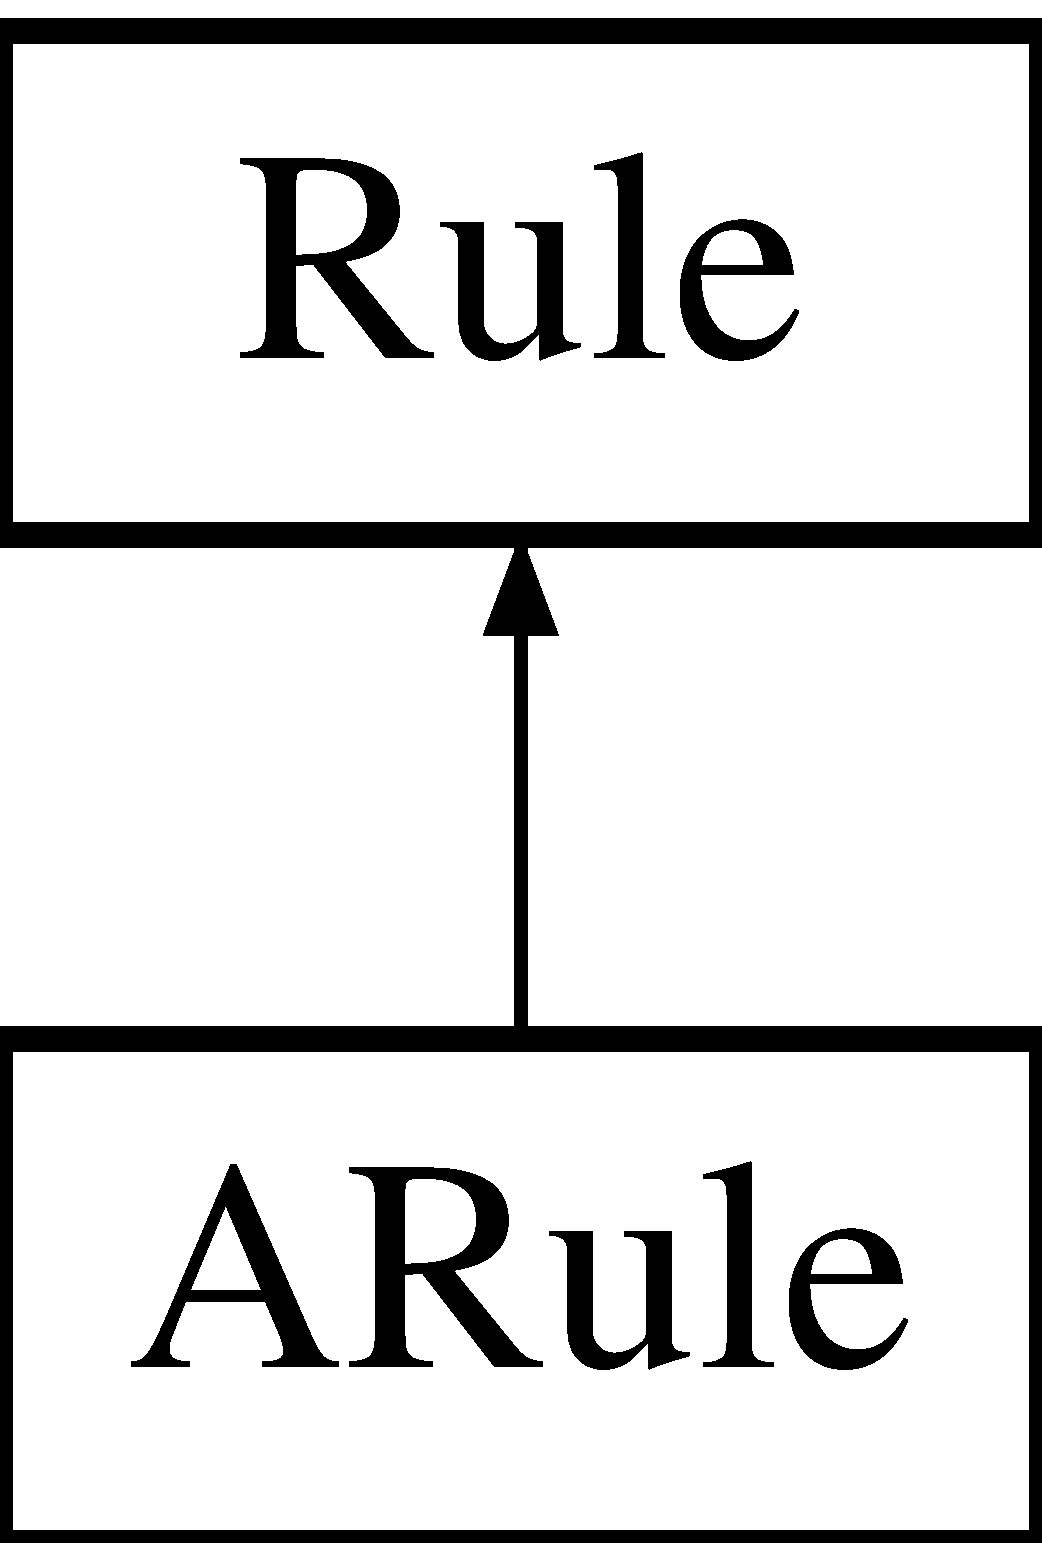
\includegraphics[height=2.000000cm]{class_d_t_r_1_1_a_rule}
\end{center}
\end{figure}
\subsection*{Additional Inherited Members}


\subsection{Detailed Description}
This class describes an asymmetrical rule.

An asymmetrical rule represents a two layers rule for which inverting layer1 and layer2 implies that the value of rule change. For example minimum enclosure rule is assymetrical.

Typical arules are\-: {\itshape min\-Extension, min\-Enclosure, min\-Length\-Enclosure, min\-Width\-Enclosure, line\-Extension, min\-Gate\-Extension, min\-Gate\-Enclosure} 
\hypertarget{class_open_chams_1_1_bloc}{\section{Bloc Class Reference}
\label{class_open_chams_1_1_bloc}\index{Bloc@{Bloc}}
}
Inheritance diagram for Bloc\-:\begin{figure}[H]
\begin{center}
\leavevmode
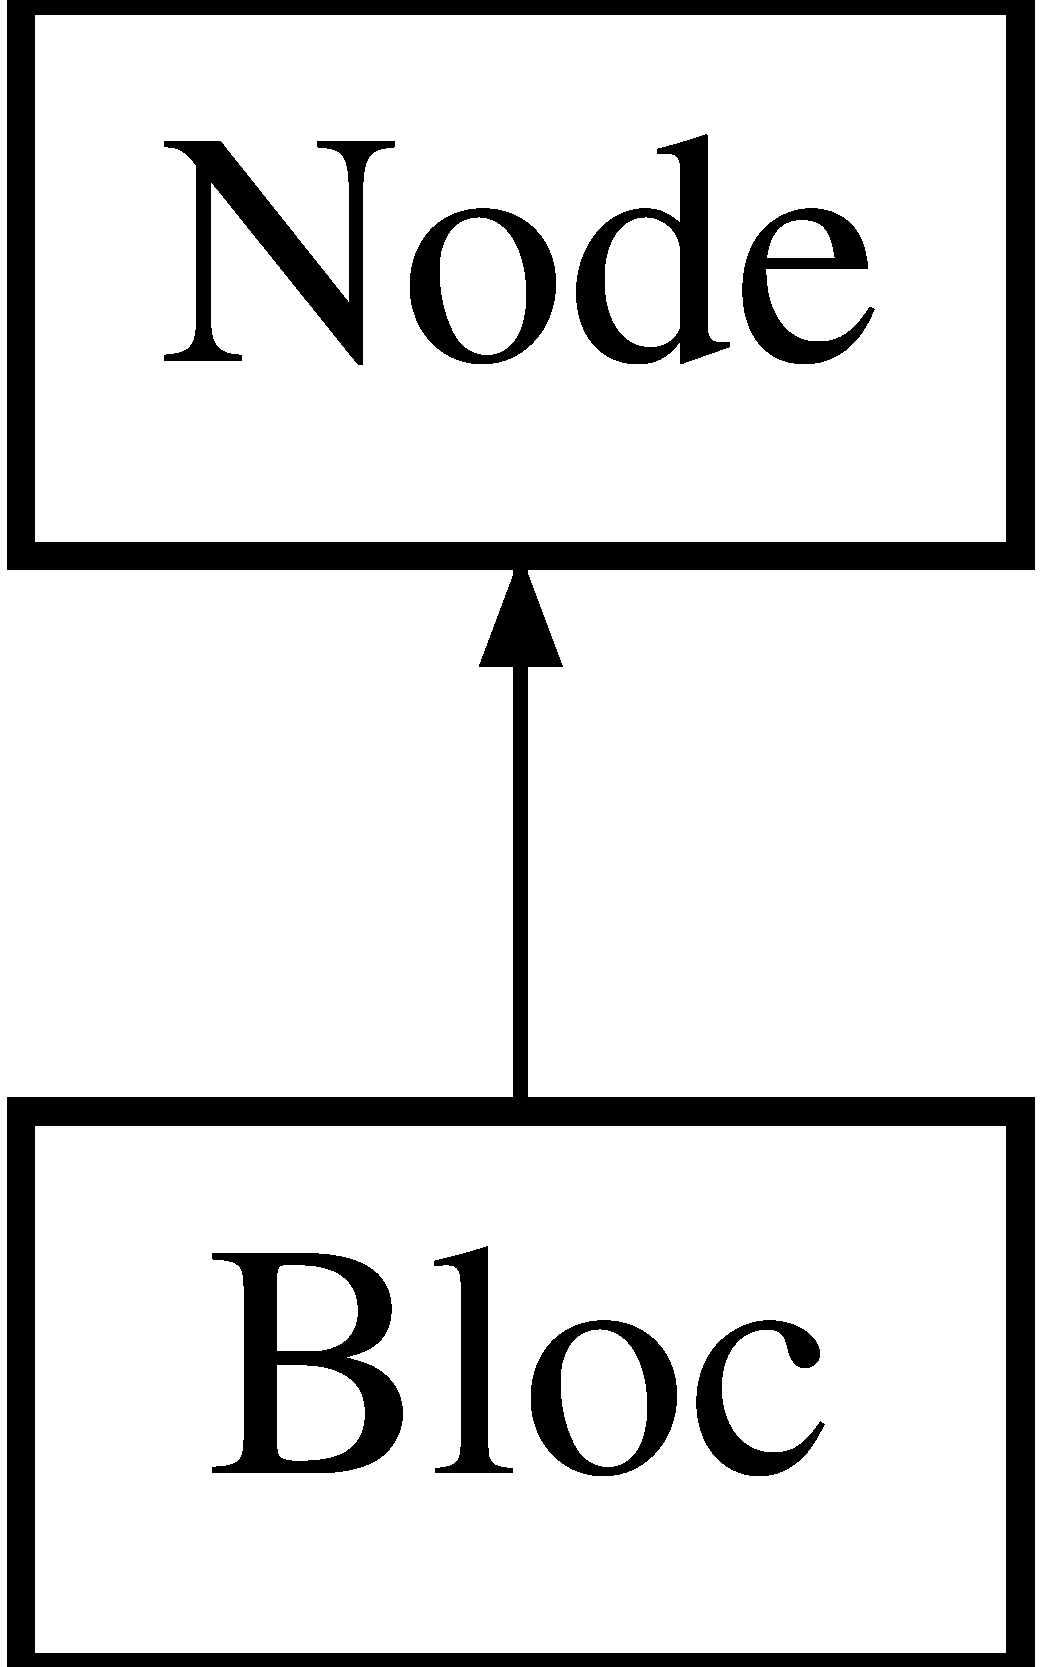
\includegraphics[height=2.000000cm]{class_open_chams_1_1_bloc}
\end{center}
\end{figure}
\subsection*{Public Member Functions}
\begin{DoxyCompactItemize}
\item 
\hyperlink{class_open_chams_1_1_bloc_a06a4a848ddb493d0026abe2b307aa94a}{Bloc} (const std\-::string \&bloc\-Name, Position pos=Node\-::\-N\-O\-N\-E, \hyperlink{class_open_chams_1_1_node}{Node} $\ast$parent=N\-U\-L\-L)
\begin{DoxyCompactList}\small\item\em creates a new bloc. \end{DoxyCompactList}\end{DoxyCompactItemize}


\subsection{Detailed Description}
This class describes a bloc of the placement tree. 

\subsection{Constructor \& Destructor Documentation}
\hypertarget{class_open_chams_1_1_bloc_a06a4a848ddb493d0026abe2b307aa94a}{\index{Open\-Chams\-::\-Bloc@{Open\-Chams\-::\-Bloc}!Bloc@{Bloc}}
\index{Bloc@{Bloc}!OpenChams::Bloc@{Open\-Chams\-::\-Bloc}}
\subsubsection[{Bloc}]{\setlength{\rightskip}{0pt plus 5cm}{\bf Bloc} (
\begin{DoxyParamCaption}
\item[{const std\-::string \&}]{bloc\-Name, }
\item[{Position}]{pos = {\ttfamily Node\-:\-:NONE}, }
\item[{{\bf Node} $\ast$}]{parent = {\ttfamily NULL}}
\end{DoxyParamCaption}
)}}\label{class_open_chams_1_1_bloc_a06a4a848ddb493d0026abe2b307aa94a}


creates a new bloc. 


\begin{DoxyParams}{Parameters}
{\em bloc\-Name} & the name of the bloc \\
\hline
{\em position} & the position of the bloc (default value\-: N\-O\-N\-E) \\
\hline
{\em parent} & the parent node of the node (default value\-: N\-U\-L\-L) \\
\hline
\end{DoxyParams}

\hypertarget{class_s_p_i_c_e_1_1_capacitor}{\section{Capacitor Class Reference}
\label{class_s_p_i_c_e_1_1_capacitor}\index{Capacitor@{Capacitor}}
}
Inheritance diagram for Capacitor\-:\begin{figure}[H]
\begin{center}
\leavevmode
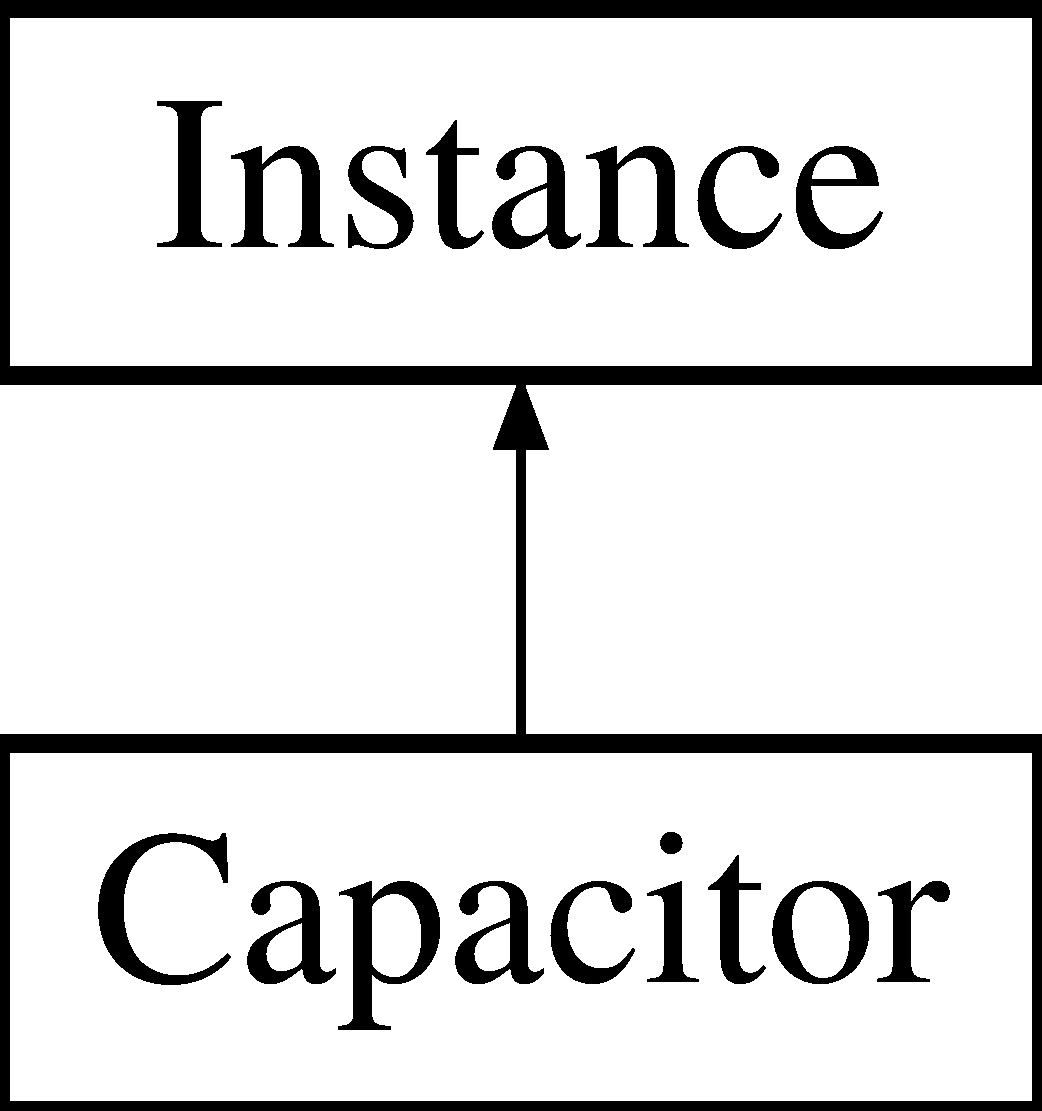
\includegraphics[height=2.000000cm]{class_s_p_i_c_e_1_1_capacitor}
\end{center}
\end{figure}
\subsection*{Public Member Functions}
\begin{DoxyCompactItemize}
\item 
\hyperlink{class_s_p_i_c_e_1_1_capacitor_af3141143353c1a45fb2f2f35d3ddd28d}{Capacitor} (std\-::string name, std\-::string pos, std\-::string neg, std\-::string value)
\begin{DoxyCompactList}\small\item\em creates a new capacitor. \end{DoxyCompactList}\item 
\hypertarget{class_s_p_i_c_e_1_1_capacitor_a8b4ab73ed1d99c533aa22af0a37ebb0d}{std\-::string \hyperlink{class_s_p_i_c_e_1_1_capacitor_a8b4ab73ed1d99c533aa22af0a37ebb0d}{get\-Negative} ()}\label{class_s_p_i_c_e_1_1_capacitor_a8b4ab73ed1d99c533aa22af0a37ebb0d}

\begin{DoxyCompactList}\small\item\em returns the negative connector of the capacitor. \end{DoxyCompactList}\item 
\hypertarget{class_s_p_i_c_e_1_1_capacitor_a1adb347b9a2c2da556e4417ab0eec0e1}{std\-::string \hyperlink{class_s_p_i_c_e_1_1_capacitor_a1adb347b9a2c2da556e4417ab0eec0e1}{get\-Positive} ()}\label{class_s_p_i_c_e_1_1_capacitor_a1adb347b9a2c2da556e4417ab0eec0e1}

\begin{DoxyCompactList}\small\item\em returns the positive connector of the capacitor. \end{DoxyCompactList}\item 
\hypertarget{class_s_p_i_c_e_1_1_capacitor_a4c052cb2622c580a250b2c783a436882}{std\-::string \hyperlink{class_s_p_i_c_e_1_1_capacitor_a4c052cb2622c580a250b2c783a436882}{get\-Value} ()}\label{class_s_p_i_c_e_1_1_capacitor_a4c052cb2622c580a250b2c783a436882}

\begin{DoxyCompactList}\small\item\em returns the value of the capacitor. \end{DoxyCompactList}\end{DoxyCompactItemize}


\subsection{Detailed Description}
This class describes a capacitor which is a specialized instance which has a positive and a negative connector and a value. 

\subsection{Constructor \& Destructor Documentation}
\hypertarget{class_s_p_i_c_e_1_1_capacitor_af3141143353c1a45fb2f2f35d3ddd28d}{\index{S\-P\-I\-C\-E\-::\-Capacitor@{S\-P\-I\-C\-E\-::\-Capacitor}!Capacitor@{Capacitor}}
\index{Capacitor@{Capacitor}!SPICE::Capacitor@{S\-P\-I\-C\-E\-::\-Capacitor}}
\subsubsection[{Capacitor}]{\setlength{\rightskip}{0pt plus 5cm}{\bf Capacitor} (
\begin{DoxyParamCaption}
\item[{std\-::string}]{name, }
\item[{std\-::string}]{pos, }
\item[{std\-::string}]{neg, }
\item[{std\-::string}]{value}
\end{DoxyParamCaption}
)\hspace{0.3cm}{\ttfamily [inline]}}}\label{class_s_p_i_c_e_1_1_capacitor_af3141143353c1a45fb2f2f35d3ddd28d}


creates a new capacitor. 


\begin{DoxyParams}{Parameters}
{\em name} & the name of the capacitor. \\
\hline
{\em pos} & the positive connector of the capacitor. \\
\hline
{\em neg} & the negative connector of the capacitor. \\
\hline
{\em value} & the value of the capacitor. \\
\hline
\end{DoxyParams}

\hypertarget{class_c_i_f_1_1_circuit}{}\section{Circuit Class Reference}
\label{class_c_i_f_1_1_circuit}\index{Circuit@{Circuit}}
\subsection*{Public Member Functions}
\begin{DoxyCompactItemize}
\item 
bool \hyperlink{class_c_i_f_1_1_circuit_a5b37e86206e2a128ba6db4987dc09a39}{add\+Polygon} (\hyperlink{class_c_i_f_1_1_polygon}{Polygon} $\ast$)
\begin{DoxyCompactList}\small\item\em adds a \hyperlink{class_c_i_f_1_1_polygon}{Polygon} to the \hyperlink{class_c_i_f_1_1_circuit}{Circuit}. \end{DoxyCompactList}\item 
\hyperlink{class_c_i_f_1_1_circuit_ad434e573e0ce37a59f39fa74fe9bfb79}{Circuit} (std\+::string name, std\+::string unit, double scale)
\begin{DoxyCompactList}\small\item\em creates a new \hyperlink{class_c_i_f_1_1_circuit}{Circuit} \end{DoxyCompactList}\item 
bool \hyperlink{class_c_i_f_1_1_circuit_a90c823b70c4984f302c19ceca604d101}{write\+To\+File} (std\+::string)
\begin{DoxyCompactList}\small\item\em writes the database to file. \end{DoxyCompactList}\end{DoxyCompactItemize}


\subsection{Detailed Description}
This class contains all C\+IF circuit informations such as the name, the unit used, the scale and the list of all Polygons. 

\subsection{Constructor \& Destructor Documentation}
\mbox{\Hypertarget{class_c_i_f_1_1_circuit_ad434e573e0ce37a59f39fa74fe9bfb79}\label{class_c_i_f_1_1_circuit_ad434e573e0ce37a59f39fa74fe9bfb79}} 
\index{C\+I\+F\+::\+Circuit@{C\+I\+F\+::\+Circuit}!Circuit@{Circuit}}
\index{Circuit@{Circuit}!C\+I\+F\+::\+Circuit@{C\+I\+F\+::\+Circuit}}
\subsubsection{\texorpdfstring{Circuit()}{Circuit()}}
{\footnotesize\ttfamily \hyperlink{class_c_i_f_1_1_circuit}{Circuit} (\begin{DoxyParamCaption}\item[{std\+::string}]{name,  }\item[{std\+::string}]{unit,  }\item[{double}]{scale }\end{DoxyParamCaption})}



creates a new \hyperlink{class_c_i_f_1_1_circuit}{Circuit} 


\begin{DoxyParams}{Parameters}
{\em name} & the name of the circuit. \\
\hline
{\em unit} & the unit used for all distances \& coordinates. \\
\hline
{\em scale} & the scale used to convert DB unit to real unit (specified by the unit). \\
\hline
\end{DoxyParams}


\subsection{Member Function Documentation}
\mbox{\Hypertarget{class_c_i_f_1_1_circuit_a5b37e86206e2a128ba6db4987dc09a39}\label{class_c_i_f_1_1_circuit_a5b37e86206e2a128ba6db4987dc09a39}} 
\index{C\+I\+F\+::\+Circuit@{C\+I\+F\+::\+Circuit}!add\+Polygon@{add\+Polygon}}
\index{add\+Polygon@{add\+Polygon}!C\+I\+F\+::\+Circuit@{C\+I\+F\+::\+Circuit}}
\subsubsection{\texorpdfstring{add\+Polygon()}{addPolygon()}}
{\footnotesize\ttfamily bool add\+Polygon (\begin{DoxyParamCaption}\item[{\hyperlink{class_c_i_f_1_1_polygon}{Polygon} $\ast$}]{polygon }\end{DoxyParamCaption})}



adds a \hyperlink{class_c_i_f_1_1_polygon}{Polygon} to the \hyperlink{class_c_i_f_1_1_circuit}{Circuit}. 


\begin{DoxyParams}{Parameters}
{\em polygon} & the \hyperlink{class_c_i_f_1_1_polygon}{Polygon} object to add. \\
\hline
\end{DoxyParams}
\mbox{\Hypertarget{class_c_i_f_1_1_circuit_a90c823b70c4984f302c19ceca604d101}\label{class_c_i_f_1_1_circuit_a90c823b70c4984f302c19ceca604d101}} 
\index{C\+I\+F\+::\+Circuit@{C\+I\+F\+::\+Circuit}!write\+To\+File@{write\+To\+File}}
\index{write\+To\+File@{write\+To\+File}!C\+I\+F\+::\+Circuit@{C\+I\+F\+::\+Circuit}}
\subsubsection{\texorpdfstring{write\+To\+File()}{writeToFile()}}
{\footnotesize\ttfamily bool write\+To\+File (\begin{DoxyParamCaption}\item[{std\+::string}]{filename }\end{DoxyParamCaption})}



writes the database to file. 


\begin{DoxyParams}{Parameters}
{\em filename} & the destination file name.\\
\hline
\end{DoxyParams}
\begin{DoxyNote}{Note}
When driving file, current date and time are used to define date in generated C\+IF file. 
\end{DoxyNote}

\hypertarget{class_open_chams_1_1_circuit}{\section{Circuit Class Reference}
\label{class_open_chams_1_1_circuit}\index{Circuit@{Circuit}}
}
\subsection*{Public Member Functions}
\begin{DoxyCompactItemize}
\item 
void \hyperlink{class_open_chams_1_1_circuit_a7c1c09f44cf215dc17d3dd2518e32389}{add\-Simul\-Model} (unsigned, \hyperlink{class_open_chams_1_1_simul_model_a450696a95d6cb29d7723838846948340}{Simul\-Model\-::\-Base}, \hyperlink{class_open_chams_1_1_simul_model_a2256f5bba1c1c69a92b933aa501df470}{Simul\-Model\-::\-Version}, std\-::string)
\begin{DoxyCompactList}\small\item\em adds a \hyperlink{class_open_chams_1_1_simul_model}{Simul\-Model} to the circuit. \end{DoxyCompactList}\item 
void \hyperlink{class_open_chams_1_1_circuit_a55234deef1d06c617a519a575ce33608}{add\-Sub\-Circuit\-Path} (std\-::string)
\begin{DoxyCompactList}\small\item\em adds a path to circuit's subcircuit paths list. \end{DoxyCompactList}\item 
\hyperlink{class_open_chams_1_1_layout}{Layout} $\ast$ \hyperlink{class_open_chams_1_1_circuit_a725a691b0117c4b913b54e7bfd92832f}{create\-Layout} ()
\begin{DoxyCompactList}\small\item\em creates a new empty layout and associates it to the circuit. \end{DoxyCompactList}\item 
\hyperlink{class_open_chams_1_1_netlist}{Netlist} $\ast$ \hyperlink{class_open_chams_1_1_circuit_a3f11671c7ea7b4e2cc3487bd7954b667}{create\-Netlist} ()
\begin{DoxyCompactList}\small\item\em creates a new empty netlist and associates it to the circuit. \end{DoxyCompactList}\item 
\hyperlink{class_open_chams_1_1_schematic}{Schematic} $\ast$ \hyperlink{class_open_chams_1_1_circuit_a57a79a9916df4512648bb195decb7250}{create\-Schematic} ()
\begin{DoxyCompactList}\small\item\em creates a new empty schematic and associates it to the circuit. \end{DoxyCompactList}\item 
\hypertarget{class_open_chams_1_1_circuit_a403a908943f9a3e820fd25a86d00531d}{\hyperlink{class_open_chams_1_1_layout}{Layout} $\ast$ \hyperlink{class_open_chams_1_1_circuit_a403a908943f9a3e820fd25a86d00531d}{get\-Layout} ()}\label{class_open_chams_1_1_circuit_a403a908943f9a3e820fd25a86d00531d}

\begin{DoxyCompactList}\small\item\em returns the \hyperlink{class_open_chams_1_1_layout}{Layout} object associated to the circuit or N\-U\-L\-L if it does not exist. \end{DoxyCompactList}\item 
\hypertarget{class_open_chams_1_1_circuit_a2858c0c4e8b5108f041237cf5a802029}{const std\-::string \& \hyperlink{class_open_chams_1_1_circuit_a2858c0c4e8b5108f041237cf5a802029}{get\-Name} ()}\label{class_open_chams_1_1_circuit_a2858c0c4e8b5108f041237cf5a802029}

\begin{DoxyCompactList}\small\item\em returns the name of the circuit. \end{DoxyCompactList}\item 
\hypertarget{class_open_chams_1_1_circuit_a4085d6a7b6958ffdd7ab5df7e6d6e53f}{\hyperlink{class_open_chams_1_1_netlist}{Netlist} $\ast$ \hyperlink{class_open_chams_1_1_circuit_a4085d6a7b6958ffdd7ab5df7e6d6e53f}{get\-Netlist} ()}\label{class_open_chams_1_1_circuit_a4085d6a7b6958ffdd7ab5df7e6d6e53f}

\begin{DoxyCompactList}\small\item\em returns the \hyperlink{class_open_chams_1_1_netlist}{Netlist} object associated to the circuit or N\-U\-L\-L if it does not exist. \end{DoxyCompactList}\item 
\hypertarget{class_open_chams_1_1_circuit_a2e51ad4344607fc279c5c8cda4edae02}{\hyperlink{class_open_chams_1_1_parameters}{Parameters} \hyperlink{class_open_chams_1_1_circuit_a2e51ad4344607fc279c5c8cda4edae02}{get\-Parameters} ()}\label{class_open_chams_1_1_circuit_a2e51ad4344607fc279c5c8cda4edae02}

\begin{DoxyCompactList}\small\item\em returns all circuit's parameters. \end{DoxyCompactList}\item 
\hypertarget{class_open_chams_1_1_circuit_af6f967a5685ac92fe760f4eb95c8c51f}{\hyperlink{class_open_chams_1_1_schematic}{Schematic} $\ast$ \hyperlink{class_open_chams_1_1_circuit_af6f967a5685ac92fe760f4eb95c8c51f}{get\-Schematic} ()}\label{class_open_chams_1_1_circuit_af6f967a5685ac92fe760f4eb95c8c51f}

\begin{DoxyCompactList}\small\item\em returns the \hyperlink{class_open_chams_1_1_schematic}{Schematic} object associated to the circuit or N\-U\-L\-L if it does not exist. \end{DoxyCompactList}\item 
\hypertarget{class_open_chams_1_1_circuit_a0ce52bc8747f684ec0123faa8ff97b6d}{\hyperlink{class_open_chams_1_1_sizing}{Sizing} $\ast$ \hyperlink{class_open_chams_1_1_circuit_a0ce52bc8747f684ec0123faa8ff97b6d}{get\-Sizing} ()}\label{class_open_chams_1_1_circuit_a0ce52bc8747f684ec0123faa8ff97b6d}

\begin{DoxyCompactList}\small\item\em returns the \hyperlink{class_open_chams_1_1_sizing}{Sizing} object associated to the circuit or N\-U\-L\-L if it does not exist. \end{DoxyCompactList}\item 
\hypertarget{class_open_chams_1_1_circuit_a3538c326d799dd26fbb17c4ac6c4647e}{const std\-::string \& \hyperlink{class_open_chams_1_1_circuit_a3538c326d799dd26fbb17c4ac6c4647e}{get\-Techno} ()}\label{class_open_chams_1_1_circuit_a3538c326d799dd26fbb17c4ac6c4647e}

\begin{DoxyCompactList}\small\item\em returns the technology. \end{DoxyCompactList}\item 
const std\-::string \& \hyperlink{class_open_chams_1_1_circuit_a6650bf10e394fe2d6fa1d50e247da296}{get\-Value} (const std\-::string \&)
\begin{DoxyCompactList}\small\item\em returns the value of the circuit's parameter named {\ttfamily name}. \end{DoxyCompactList}\item 
void \hyperlink{class_open_chams_1_1_circuit_a4babcbc5b9f7797cc0befb675d5f538c}{set\-Layout} (\hyperlink{class_open_chams_1_1_layout}{Layout} $\ast$)
\begin{DoxyCompactList}\small\item\em sets the circuit's layout. \end{DoxyCompactList}\item 
void \hyperlink{class_open_chams_1_1_circuit_ab065572c5c1d9beb304324f2d2d8b525}{set\-Sizing} (\hyperlink{class_open_chams_1_1_sizing}{Sizing} $\ast$)
\begin{DoxyCompactList}\small\item\em sets the circuit's sizing. \end{DoxyCompactList}\item 
bool \hyperlink{class_open_chams_1_1_circuit_a2eb07935ec946a07edcee2255b781193}{write\-To\-File} (std\-::string file\-Path)
\begin{DoxyCompactList}\small\item\em writes the database to file. \end{DoxyCompactList}\end{DoxyCompactItemize}
\subsection*{Static Public Member Functions}
\begin{DoxyCompactItemize}
\item 
static \hyperlink{class_open_chams_1_1_circuit}{Circuit} $\ast$ \hyperlink{class_open_chams_1_1_circuit_ad0aa3183bdea59e62f69c295026b7fe7}{read\-From\-File} (const std\-::string file\-Path)
\begin{DoxyCompactList}\small\item\em creates and returns a \hyperlink{class_open_chams_1_1_circuit}{Circuit} object based on a database source file. \end{DoxyCompactList}\end{DoxyCompactItemize}


\subsection{Detailed Description}
This class is the root class whihch means that having this object in hand allows to get/set any information contained in the Open\-Chams file parsed/drived. 

\subsection{Member Function Documentation}
\hypertarget{class_open_chams_1_1_circuit_a7c1c09f44cf215dc17d3dd2518e32389}{\index{Open\-Chams\-::\-Circuit@{Open\-Chams\-::\-Circuit}!add\-Simul\-Model@{add\-Simul\-Model}}
\index{add\-Simul\-Model@{add\-Simul\-Model}!OpenChams::Circuit@{Open\-Chams\-::\-Circuit}}
\subsubsection[{add\-Simul\-Model}]{\setlength{\rightskip}{0pt plus 5cm}void add\-Simul\-Model (
\begin{DoxyParamCaption}
\item[{unsigned}]{id, }
\item[{{\bf Simul\-Model\-::\-Base}}]{base, }
\item[{{\bf Simul\-Model\-::\-Version}}]{version, }
\item[{std\-::string}]{file\-Path}
\end{DoxyParamCaption}
)}}\label{class_open_chams_1_1_circuit_a7c1c09f44cf215dc17d3dd2518e32389}


adds a \hyperlink{class_open_chams_1_1_simul_model}{Simul\-Model} to the circuit. 


\begin{DoxyParams}{Parameters}
{\em id} & the simulation model id. \\
\hline
{\em base} & the simulation model base. \\
\hline
{\em version} & the simulation model version. \\
\hline
{\em file\-Path} & the path to the netlist used by simulation model. \\
\hline
\end{DoxyParams}
\hypertarget{class_open_chams_1_1_circuit_a55234deef1d06c617a519a575ce33608}{\index{Open\-Chams\-::\-Circuit@{Open\-Chams\-::\-Circuit}!add\-Sub\-Circuit\-Path@{add\-Sub\-Circuit\-Path}}
\index{add\-Sub\-Circuit\-Path@{add\-Sub\-Circuit\-Path}!OpenChams::Circuit@{Open\-Chams\-::\-Circuit}}
\subsubsection[{add\-Sub\-Circuit\-Path}]{\setlength{\rightskip}{0pt plus 5cm}void add\-Sub\-Circuit\-Path (
\begin{DoxyParamCaption}
\item[{std\-::string}]{path}
\end{DoxyParamCaption}
)\hspace{0.3cm}{\ttfamily [inline]}}}\label{class_open_chams_1_1_circuit_a55234deef1d06c617a519a575ce33608}


adds a path to circuit's subcircuit paths list. 

Sub\-Circuit\-Paths are used to define where to search the xml file describing subcircuits used in current circuit. \hypertarget{class_open_chams_1_1_circuit_a725a691b0117c4b913b54e7bfd92832f}{\index{Open\-Chams\-::\-Circuit@{Open\-Chams\-::\-Circuit}!create\-Layout@{create\-Layout}}
\index{create\-Layout@{create\-Layout}!OpenChams::Circuit@{Open\-Chams\-::\-Circuit}}
\subsubsection[{create\-Layout}]{\setlength{\rightskip}{0pt plus 5cm}{\bf Layout} $\ast$ create\-Layout (
\begin{DoxyParamCaption}
{}
\end{DoxyParamCaption}
)}}\label{class_open_chams_1_1_circuit_a725a691b0117c4b913b54e7bfd92832f}


creates a new empty layout and associates it to the circuit. 

\begin{DoxyReturn}{Returns}
the newly created layout. 
\end{DoxyReturn}
\hypertarget{class_open_chams_1_1_circuit_a3f11671c7ea7b4e2cc3487bd7954b667}{\index{Open\-Chams\-::\-Circuit@{Open\-Chams\-::\-Circuit}!create\-Netlist@{create\-Netlist}}
\index{create\-Netlist@{create\-Netlist}!OpenChams::Circuit@{Open\-Chams\-::\-Circuit}}
\subsubsection[{create\-Netlist}]{\setlength{\rightskip}{0pt plus 5cm}{\bf Netlist} $\ast$ create\-Netlist (
\begin{DoxyParamCaption}
{}
\end{DoxyParamCaption}
)}}\label{class_open_chams_1_1_circuit_a3f11671c7ea7b4e2cc3487bd7954b667}


creates a new empty netlist and associates it to the circuit. 

\begin{DoxyReturn}{Returns}
the newly created netlist. 
\end{DoxyReturn}
\hypertarget{class_open_chams_1_1_circuit_a57a79a9916df4512648bb195decb7250}{\index{Open\-Chams\-::\-Circuit@{Open\-Chams\-::\-Circuit}!create\-Schematic@{create\-Schematic}}
\index{create\-Schematic@{create\-Schematic}!OpenChams::Circuit@{Open\-Chams\-::\-Circuit}}
\subsubsection[{create\-Schematic}]{\setlength{\rightskip}{0pt plus 5cm}{\bf Schematic} $\ast$ create\-Schematic (
\begin{DoxyParamCaption}
{}
\end{DoxyParamCaption}
)}}\label{class_open_chams_1_1_circuit_a57a79a9916df4512648bb195decb7250}


creates a new empty schematic and associates it to the circuit. 

\begin{DoxyReturn}{Returns}
the newly created schematic. 
\end{DoxyReturn}
\hypertarget{class_open_chams_1_1_circuit_a6650bf10e394fe2d6fa1d50e247da296}{\index{Open\-Chams\-::\-Circuit@{Open\-Chams\-::\-Circuit}!get\-Value@{get\-Value}}
\index{get\-Value@{get\-Value}!OpenChams::Circuit@{Open\-Chams\-::\-Circuit}}
\subsubsection[{get\-Value}]{\setlength{\rightskip}{0pt plus 5cm}const std\-::string \& get\-Value (
\begin{DoxyParamCaption}
\item[{const std\-::string \&}]{name}
\end{DoxyParamCaption}
)\hspace{0.3cm}{\ttfamily [inline]}}}\label{class_open_chams_1_1_circuit_a6650bf10e394fe2d6fa1d50e247da296}


returns the value of the circuit's parameter named {\ttfamily name}. 


\begin{DoxyParams}{Parameters}
{\em name} & the name of the parameter. \\
\hline
\end{DoxyParams}
\hypertarget{class_open_chams_1_1_circuit_ad0aa3183bdea59e62f69c295026b7fe7}{\index{Open\-Chams\-::\-Circuit@{Open\-Chams\-::\-Circuit}!read\-From\-File@{read\-From\-File}}
\index{read\-From\-File@{read\-From\-File}!OpenChams::Circuit@{Open\-Chams\-::\-Circuit}}
\subsubsection[{read\-From\-File}]{\setlength{\rightskip}{0pt plus 5cm}{\bf Circuit} $\ast$ read\-From\-File (
\begin{DoxyParamCaption}
\item[{const std\-::string}]{file\-Path}
\end{DoxyParamCaption}
)\hspace{0.3cm}{\ttfamily [static]}}}\label{class_open_chams_1_1_circuit_ad0aa3183bdea59e62f69c295026b7fe7}


creates and returns a \hyperlink{class_open_chams_1_1_circuit}{Circuit} object based on a database source file. 


\begin{DoxyParams}{Parameters}
{\em file\-Path} & the source file name.\\
\hline
\end{DoxyParams}
\begin{DoxyReturn}{Returns}
the newly created \hyperlink{class_open_chams_1_1_circuit}{Circuit}. 
\end{DoxyReturn}
\hypertarget{class_open_chams_1_1_circuit_a4babcbc5b9f7797cc0befb675d5f538c}{\index{Open\-Chams\-::\-Circuit@{Open\-Chams\-::\-Circuit}!set\-Layout@{set\-Layout}}
\index{set\-Layout@{set\-Layout}!OpenChams::Circuit@{Open\-Chams\-::\-Circuit}}
\subsubsection[{set\-Layout}]{\setlength{\rightskip}{0pt plus 5cm}void set\-Layout (
\begin{DoxyParamCaption}
\item[{{\bf Layout} $\ast$}]{layout}
\end{DoxyParamCaption}
)\hspace{0.3cm}{\ttfamily [inline]}}}\label{class_open_chams_1_1_circuit_a4babcbc5b9f7797cc0befb675d5f538c}


sets the circuit's layout. 


\begin{DoxyParams}{Parameters}
{\em layout} & the layout of the circuit. \\
\hline
\end{DoxyParams}
\hypertarget{class_open_chams_1_1_circuit_ab065572c5c1d9beb304324f2d2d8b525}{\index{Open\-Chams\-::\-Circuit@{Open\-Chams\-::\-Circuit}!set\-Sizing@{set\-Sizing}}
\index{set\-Sizing@{set\-Sizing}!OpenChams::Circuit@{Open\-Chams\-::\-Circuit}}
\subsubsection[{set\-Sizing}]{\setlength{\rightskip}{0pt plus 5cm}void set\-Sizing (
\begin{DoxyParamCaption}
\item[{{\bf Sizing} $\ast$}]{sizing}
\end{DoxyParamCaption}
)\hspace{0.3cm}{\ttfamily [inline]}}}\label{class_open_chams_1_1_circuit_ab065572c5c1d9beb304324f2d2d8b525}


sets the circuit's sizing. 


\begin{DoxyParams}{Parameters}
{\em sizing} & the sizing of the circuit. \\
\hline
\end{DoxyParams}
\hypertarget{class_open_chams_1_1_circuit_a2eb07935ec946a07edcee2255b781193}{\index{Open\-Chams\-::\-Circuit@{Open\-Chams\-::\-Circuit}!write\-To\-File@{write\-To\-File}}
\index{write\-To\-File@{write\-To\-File}!OpenChams::Circuit@{Open\-Chams\-::\-Circuit}}
\subsubsection[{write\-To\-File}]{\setlength{\rightskip}{0pt plus 5cm}bool write\-To\-File (
\begin{DoxyParamCaption}
\item[{std\-::string}]{file\-Path}
\end{DoxyParamCaption}
)}}\label{class_open_chams_1_1_circuit_a2eb07935ec946a07edcee2255b781193}


writes the database to file. 


\begin{DoxyParams}{Parameters}
{\em file\-Path} & the destination file. \\
\hline
\end{DoxyParams}

\hypertarget{class_s_p_i_c_e_1_1_circuit}{}\section{Circuit Class Reference}
\label{class_s_p_i_c_e_1_1_circuit}\index{Circuit@{Circuit}}
\subsection*{Public Member Functions}
\begin{DoxyCompactItemize}
\item 
void \hyperlink{class_s_p_i_c_e_1_1_circuit_a30fc53c4da54215fdec3ab1b96ea1943}{add\+Include} (std\+::string)
\begin{DoxyCompactList}\small\item\em adds an include to the circuit. \end{DoxyCompactList}\item 
void \hyperlink{class_s_p_i_c_e_1_1_circuit_a7bb4a4532643568ab1ac2c229185a88e}{add\+Instance} (\hyperlink{class_s_p_i_c_e_1_1_instance}{Instance} $\ast$)
\begin{DoxyCompactList}\small\item\em adds an instance to the circuit. \end{DoxyCompactList}\item 
void \hyperlink{class_s_p_i_c_e_1_1_circuit_a49939060cc1cb8e4bfaf003025032096}{add\+Library} (std\+::string file, std\+::string type=\char`\"{}\char`\"{})
\begin{DoxyCompactList}\small\item\em adds a library to the circuit. \end{DoxyCompactList}\item 
void \hyperlink{class_s_p_i_c_e_1_1_circuit_a1abe34b48e2b6e1834a143fdef159cb9}{add\+Option} (std\+::string, std\+::string)
\begin{DoxyCompactList}\small\item\em adds an option to the circuit. \end{DoxyCompactList}\item 
void \hyperlink{class_s_p_i_c_e_1_1_circuit_ab3ab147a16bc490ce96db905a4ca271c}{add\+Parameter} (std\+::string, std\+::string)
\begin{DoxyCompactList}\small\item\em adds a parameter to the circuit. \end{DoxyCompactList}\item 
void \hyperlink{class_s_p_i_c_e_1_1_circuit_a627cf18c2763bb59f3d7e5142873251c}{add\+Source} (\hyperlink{class_s_p_i_c_e_1_1_source}{Source} $\ast$)
\begin{DoxyCompactList}\small\item\em adds a source to the circuit. \end{DoxyCompactList}\item 
\hyperlink{class_s_p_i_c_e_1_1_subckt}{Subckt} $\ast$ \hyperlink{class_s_p_i_c_e_1_1_circuit_a0d1352e46d4537ce1e5f651de40e91a6}{add\+Subckt} (std\+::string)
\begin{DoxyCompactList}\small\item\em adds a subcircuit to the circuit. \end{DoxyCompactList}\item 
\mbox{\Hypertarget{class_s_p_i_c_e_1_1_circuit_a2210ebc37eee536dbe9b44a89690256c}\label{class_s_p_i_c_e_1_1_circuit_a2210ebc37eee536dbe9b44a89690256c}} 
\hyperlink{class_s_p_i_c_e_1_1_circuit_a2210ebc37eee536dbe9b44a89690256c}{Circuit} ()
\begin{DoxyCompactList}\small\item\em creates a new circuit \end{DoxyCompactList}\item 
\mbox{\Hypertarget{class_s_p_i_c_e_1_1_circuit_a312beaf640e84589e6644820355c8ed6}\label{class_s_p_i_c_e_1_1_circuit_a312beaf640e84589e6644820355c8ed6}} 
const string\+\_\+vector \& \hyperlink{class_s_p_i_c_e_1_1_circuit_a312beaf640e84589e6644820355c8ed6}{get\+Includes} ()
\begin{DoxyCompactList}\small\item\em returns the includes of the circuit. \end{DoxyCompactList}\item 
\mbox{\Hypertarget{class_s_p_i_c_e_1_1_circuit_a8e6e58ffab876152a740092520c35d73}\label{class_s_p_i_c_e_1_1_circuit_a8e6e58ffab876152a740092520c35d73}} 
const std\+::vector$<$ \hyperlink{class_s_p_i_c_e_1_1_instance}{Instance} $\ast$ $>$ \& \hyperlink{class_s_p_i_c_e_1_1_circuit_a8e6e58ffab876152a740092520c35d73}{get\+Instances} ()
\begin{DoxyCompactList}\small\item\em returns the instances of the circuit. \end{DoxyCompactList}\item 
\mbox{\Hypertarget{class_s_p_i_c_e_1_1_circuit_a3e6a71a711e4796470f1a2a1dc42aef6}\label{class_s_p_i_c_e_1_1_circuit_a3e6a71a711e4796470f1a2a1dc42aef6}} 
const strpair\+\_\+vector \& \hyperlink{class_s_p_i_c_e_1_1_circuit_a3e6a71a711e4796470f1a2a1dc42aef6}{get\+Libraries} ()
\begin{DoxyCompactList}\small\item\em returns the libraries of the circuit. \end{DoxyCompactList}\item 
\mbox{\Hypertarget{class_s_p_i_c_e_1_1_circuit_a4ee11ef79ef893c5621e0e7d26a7f9a7}\label{class_s_p_i_c_e_1_1_circuit_a4ee11ef79ef893c5621e0e7d26a7f9a7}} 
const strings\+\_\+map \& \hyperlink{class_s_p_i_c_e_1_1_circuit_a4ee11ef79ef893c5621e0e7d26a7f9a7}{get\+Options} ()
\begin{DoxyCompactList}\small\item\em returns the options of the circuit. \end{DoxyCompactList}\item 
\mbox{\Hypertarget{class_s_p_i_c_e_1_1_circuit_a4c46676f9ead2db537a0dd963b4f08f1}\label{class_s_p_i_c_e_1_1_circuit_a4c46676f9ead2db537a0dd963b4f08f1}} 
const strings\+\_\+map \& \hyperlink{class_s_p_i_c_e_1_1_circuit_a4c46676f9ead2db537a0dd963b4f08f1}{get\+Parameters} ()
\begin{DoxyCompactList}\small\item\em returns the parameters of the circuit. \end{DoxyCompactList}\item 
\mbox{\Hypertarget{class_s_p_i_c_e_1_1_circuit_ac18caa525ed386c44874ee643c88e27b}\label{class_s_p_i_c_e_1_1_circuit_ac18caa525ed386c44874ee643c88e27b}} 
const std\+::vector$<$ \hyperlink{class_s_p_i_c_e_1_1_source}{Source} $\ast$ $>$ \& \hyperlink{class_s_p_i_c_e_1_1_circuit_ac18caa525ed386c44874ee643c88e27b}{get\+Sources} ()
\begin{DoxyCompactList}\small\item\em returns the sources of the circuit. \end{DoxyCompactList}\item 
\mbox{\Hypertarget{class_s_p_i_c_e_1_1_circuit_adcc4ca0de68f8ee05f0d5db3b7604930}\label{class_s_p_i_c_e_1_1_circuit_adcc4ca0de68f8ee05f0d5db3b7604930}} 
const std\+::vector$<$ \hyperlink{class_s_p_i_c_e_1_1_subckt}{Subckt} $\ast$ $>$ \& \hyperlink{class_s_p_i_c_e_1_1_circuit_adcc4ca0de68f8ee05f0d5db3b7604930}{get\+Subckts} ()
\begin{DoxyCompactList}\small\item\em returns the subckts of the circuit. \end{DoxyCompactList}\item 
\mbox{\Hypertarget{class_s_p_i_c_e_1_1_circuit_ad19721dd878c04c854a72af12d785741}\label{class_s_p_i_c_e_1_1_circuit_ad19721dd878c04c854a72af12d785741}} 
std\+::string \hyperlink{class_s_p_i_c_e_1_1_circuit_ad19721dd878c04c854a72af12d785741}{get\+Title} ()
\begin{DoxyCompactList}\small\item\em returns the title of the circuit. \end{DoxyCompactList}\item 
void \hyperlink{class_s_p_i_c_e_1_1_circuit_a798df9ebd558e22c85eeceb5202e3123}{set\+Title} (std\+::string)
\begin{DoxyCompactList}\small\item\em sets the title of the circuit. \end{DoxyCompactList}\end{DoxyCompactItemize}


\subsection{Detailed Description}
This class is the root class which means that having this object in hand allows to get/set any information contained in the Spice file parsed/drived. 

\subsection{Member Function Documentation}
\mbox{\Hypertarget{class_s_p_i_c_e_1_1_circuit_a30fc53c4da54215fdec3ab1b96ea1943}\label{class_s_p_i_c_e_1_1_circuit_a30fc53c4da54215fdec3ab1b96ea1943}} 
\index{S\+P\+I\+C\+E\+::\+Circuit@{S\+P\+I\+C\+E\+::\+Circuit}!add\+Include@{add\+Include}}
\index{add\+Include@{add\+Include}!S\+P\+I\+C\+E\+::\+Circuit@{S\+P\+I\+C\+E\+::\+Circuit}}
\subsubsection{\texorpdfstring{add\+Include()}{addInclude()}}
{\footnotesize\ttfamily void add\+Include (\begin{DoxyParamCaption}\item[{std\+::string}]{include }\end{DoxyParamCaption})\hspace{0.3cm}{\ttfamily [inline]}}



adds an include to the circuit. 


\begin{DoxyParams}{Parameters}
{\em include} & the include to add. \\
\hline
\end{DoxyParams}
\mbox{\Hypertarget{class_s_p_i_c_e_1_1_circuit_a7bb4a4532643568ab1ac2c229185a88e}\label{class_s_p_i_c_e_1_1_circuit_a7bb4a4532643568ab1ac2c229185a88e}} 
\index{S\+P\+I\+C\+E\+::\+Circuit@{S\+P\+I\+C\+E\+::\+Circuit}!add\+Instance@{add\+Instance}}
\index{add\+Instance@{add\+Instance}!S\+P\+I\+C\+E\+::\+Circuit@{S\+P\+I\+C\+E\+::\+Circuit}}
\subsubsection{\texorpdfstring{add\+Instance()}{addInstance()}}
{\footnotesize\ttfamily void add\+Instance (\begin{DoxyParamCaption}\item[{\hyperlink{class_s_p_i_c_e_1_1_instance}{Instance} $\ast$}]{instance }\end{DoxyParamCaption})\hspace{0.3cm}{\ttfamily [inline]}}



adds an instance to the circuit. 


\begin{DoxyParams}{Parameters}
{\em instance} & the instance to add. \\
\hline
\end{DoxyParams}
\mbox{\Hypertarget{class_s_p_i_c_e_1_1_circuit_a49939060cc1cb8e4bfaf003025032096}\label{class_s_p_i_c_e_1_1_circuit_a49939060cc1cb8e4bfaf003025032096}} 
\index{S\+P\+I\+C\+E\+::\+Circuit@{S\+P\+I\+C\+E\+::\+Circuit}!add\+Library@{add\+Library}}
\index{add\+Library@{add\+Library}!S\+P\+I\+C\+E\+::\+Circuit@{S\+P\+I\+C\+E\+::\+Circuit}}
\subsubsection{\texorpdfstring{add\+Library()}{addLibrary()}}
{\footnotesize\ttfamily void add\+Library (\begin{DoxyParamCaption}\item[{std\+::string}]{file,  }\item[{std\+::string}]{type = {\ttfamily \char`\"{}\char`\"{}} }\end{DoxyParamCaption})\hspace{0.3cm}{\ttfamily [inline]}}



adds a library to the circuit. 


\begin{DoxyParams}{Parameters}
{\em file} & the file describing the library to add. \\
\hline
{\em type} & the type if several exist in the same file (this argument is optionnal) \\
\hline
\end{DoxyParams}
\mbox{\Hypertarget{class_s_p_i_c_e_1_1_circuit_a1abe34b48e2b6e1834a143fdef159cb9}\label{class_s_p_i_c_e_1_1_circuit_a1abe34b48e2b6e1834a143fdef159cb9}} 
\index{S\+P\+I\+C\+E\+::\+Circuit@{S\+P\+I\+C\+E\+::\+Circuit}!add\+Option@{add\+Option}}
\index{add\+Option@{add\+Option}!S\+P\+I\+C\+E\+::\+Circuit@{S\+P\+I\+C\+E\+::\+Circuit}}
\subsubsection{\texorpdfstring{add\+Option()}{addOption()}}
{\footnotesize\ttfamily void add\+Option (\begin{DoxyParamCaption}\item[{std\+::string}]{name,  }\item[{std\+::string}]{value }\end{DoxyParamCaption})}



adds an option to the circuit. 


\begin{DoxyParams}{Parameters}
{\em name} & the name of the option. \\
\hline
{\em value} & the value of the option.\\
\hline
\end{DoxyParams}
\begin{DoxyNote}{Note}
The value is represented as a std\+::string to keep the optionnal unity. 
\end{DoxyNote}
\mbox{\Hypertarget{class_s_p_i_c_e_1_1_circuit_ab3ab147a16bc490ce96db905a4ca271c}\label{class_s_p_i_c_e_1_1_circuit_ab3ab147a16bc490ce96db905a4ca271c}} 
\index{S\+P\+I\+C\+E\+::\+Circuit@{S\+P\+I\+C\+E\+::\+Circuit}!add\+Parameter@{add\+Parameter}}
\index{add\+Parameter@{add\+Parameter}!S\+P\+I\+C\+E\+::\+Circuit@{S\+P\+I\+C\+E\+::\+Circuit}}
\subsubsection{\texorpdfstring{add\+Parameter()}{addParameter()}}
{\footnotesize\ttfamily void add\+Parameter (\begin{DoxyParamCaption}\item[{std\+::string}]{name,  }\item[{std\+::string}]{value }\end{DoxyParamCaption})}



adds a parameter to the circuit. 


\begin{DoxyParams}{Parameters}
{\em name} & the name of the parameter. \\
\hline
{\em value} & the value of the parameter.\\
\hline
\end{DoxyParams}
\begin{DoxyNote}{Note}
The value is represented as a std\+::string to keep the optionnal unity. 
\end{DoxyNote}
\mbox{\Hypertarget{class_s_p_i_c_e_1_1_circuit_a627cf18c2763bb59f3d7e5142873251c}\label{class_s_p_i_c_e_1_1_circuit_a627cf18c2763bb59f3d7e5142873251c}} 
\index{S\+P\+I\+C\+E\+::\+Circuit@{S\+P\+I\+C\+E\+::\+Circuit}!add\+Source@{add\+Source}}
\index{add\+Source@{add\+Source}!S\+P\+I\+C\+E\+::\+Circuit@{S\+P\+I\+C\+E\+::\+Circuit}}
\subsubsection{\texorpdfstring{add\+Source()}{addSource()}}
{\footnotesize\ttfamily void add\+Source (\begin{DoxyParamCaption}\item[{\hyperlink{class_s_p_i_c_e_1_1_source}{Source} $\ast$}]{source }\end{DoxyParamCaption})\hspace{0.3cm}{\ttfamily [inline]}}



adds a source to the circuit. 


\begin{DoxyParams}{Parameters}
{\em source} & the source to add. \\
\hline
\end{DoxyParams}
\mbox{\Hypertarget{class_s_p_i_c_e_1_1_circuit_a0d1352e46d4537ce1e5f651de40e91a6}\label{class_s_p_i_c_e_1_1_circuit_a0d1352e46d4537ce1e5f651de40e91a6}} 
\index{S\+P\+I\+C\+E\+::\+Circuit@{S\+P\+I\+C\+E\+::\+Circuit}!add\+Subckt@{add\+Subckt}}
\index{add\+Subckt@{add\+Subckt}!S\+P\+I\+C\+E\+::\+Circuit@{S\+P\+I\+C\+E\+::\+Circuit}}
\subsubsection{\texorpdfstring{add\+Subckt()}{addSubckt()}}
{\footnotesize\ttfamily \hyperlink{class_s_p_i_c_e_1_1_subckt}{Subckt} $\ast$ add\+Subckt (\begin{DoxyParamCaption}\item[{std\+::string}]{name }\end{DoxyParamCaption})}



adds a subcircuit to the circuit. 


\begin{DoxyParams}{Parameters}
{\em name} & the name of the subckt.\\
\hline
\end{DoxyParams}
\begin{DoxyReturn}{Returns}
the newly created \hyperlink{class_s_p_i_c_e_1_1_subckt}{Subckt}. 
\end{DoxyReturn}
\mbox{\Hypertarget{class_s_p_i_c_e_1_1_circuit_a798df9ebd558e22c85eeceb5202e3123}\label{class_s_p_i_c_e_1_1_circuit_a798df9ebd558e22c85eeceb5202e3123}} 
\index{S\+P\+I\+C\+E\+::\+Circuit@{S\+P\+I\+C\+E\+::\+Circuit}!set\+Title@{set\+Title}}
\index{set\+Title@{set\+Title}!S\+P\+I\+C\+E\+::\+Circuit@{S\+P\+I\+C\+E\+::\+Circuit}}
\subsubsection{\texorpdfstring{set\+Title()}{setTitle()}}
{\footnotesize\ttfamily void set\+Title (\begin{DoxyParamCaption}\item[{std\+::string}]{title }\end{DoxyParamCaption})\hspace{0.3cm}{\ttfamily [inline]}}



sets the title of the circuit. 


\begin{DoxyParams}{Parameters}
{\em title} & the title of the circuit \\
\hline
\end{DoxyParams}

\hypertarget{class_open_chams_1_1_net_1_1_connection}{\section{Net\-:\-:Connection Class Reference}
\label{class_open_chams_1_1_net_1_1_connection}\index{Net\-::\-Connection@{Net\-::\-Connection}}
}
\subsection*{Public Member Functions}
\begin{DoxyCompactItemize}
\item 
\hyperlink{class_open_chams_1_1_net_1_1_connection_a3e223d6a7eec0634d6b5cc90692b9cff}{Connection} (const std\-::string \&instance\-Name, const std\-::string \&connector\-Name)
\begin{DoxyCompactList}\small\item\em creates a new connection. \end{DoxyCompactList}\item 
\hypertarget{class_open_chams_1_1_net_1_1_connection_a42f70d94ed3768e0342ae2bcb09ac0ed}{const std\-::string \& \hyperlink{class_open_chams_1_1_net_1_1_connection_a42f70d94ed3768e0342ae2bcb09ac0ed}{get\-Connector\-Name} () const }\label{class_open_chams_1_1_net_1_1_connection_a42f70d94ed3768e0342ae2bcb09ac0ed}

\begin{DoxyCompactList}\small\item\em returns the name of the connector. \end{DoxyCompactList}\item 
\hypertarget{class_open_chams_1_1_net_1_1_connection_a44e43ff95d18d91abb9449a09e3c9d1f}{const std\-::string \& \hyperlink{class_open_chams_1_1_net_1_1_connection_a44e43ff95d18d91abb9449a09e3c9d1f}{get\-Instance\-Name} () const }\label{class_open_chams_1_1_net_1_1_connection_a44e43ff95d18d91abb9449a09e3c9d1f}

\begin{DoxyCompactList}\small\item\em returns the name of the instance. \end{DoxyCompactList}\end{DoxyCompactItemize}


\subsection{Detailed Description}
This class describe a \hyperlink{class_open_chams_1_1_net_1_1_connection}{Connection} in a \hyperlink{class_open_chams_1_1_net}{Net}. A connection is a couple (instance\-Name, connector\-Name) used to represent all the connectors linked to a net. 

\subsection{Constructor \& Destructor Documentation}
\hypertarget{class_open_chams_1_1_net_1_1_connection_a3e223d6a7eec0634d6b5cc90692b9cff}{\index{Open\-Chams\-::\-Net\-::\-Connection@{Open\-Chams\-::\-Net\-::\-Connection}!Connection@{Connection}}
\index{Connection@{Connection}!OpenChams::Net::Connection@{Open\-Chams\-::\-Net\-::\-Connection}}
\subsubsection[{Connection}]{\setlength{\rightskip}{0pt plus 5cm}{\bf Connection} (
\begin{DoxyParamCaption}
\item[{const std\-::string \&}]{instance\-Name, }
\item[{const std\-::string \&}]{connector\-Name}
\end{DoxyParamCaption}
)}}\label{class_open_chams_1_1_net_1_1_connection_a3e223d6a7eec0634d6b5cc90692b9cff}


creates a new connection. 


\begin{DoxyParams}{Parameters}
{\em instance\-Name} & the name of the instance. \\
\hline
{\em connector\-Name} & the name of the instance's connector. \\
\hline
\end{DoxyParams}

\hypertarget{class_open_chams_1_1_operator_1_1_constraint}{}\section{Operator\+:\+:Constraint Class Reference}
\label{class_open_chams_1_1_operator_1_1_constraint}\index{Operator\+::\+Constraint@{Operator\+::\+Constraint}}
\subsection*{Public Member Functions}
\begin{DoxyCompactItemize}
\item 
\mbox{\hyperlink{class_open_chams_1_1_operator_1_1_constraint_af99fb5eb2779471fcbad4484cf77a670}{Constraint}} (const std\+::string \&ref, const std\+::string \&ref\+Param, double factor)
\begin{DoxyCompactList}\small\item\em creates a new constraint. \end{DoxyCompactList}\item 
\mbox{\Hypertarget{class_open_chams_1_1_operator_1_1_constraint_a973fc85365f2d3f07007d88a90d7ab1d}\label{class_open_chams_1_1_operator_1_1_constraint_a973fc85365f2d3f07007d88a90d7ab1d}} 
double \mbox{\hyperlink{class_open_chams_1_1_operator_1_1_constraint_a973fc85365f2d3f07007d88a90d7ab1d}{get\+Factor}} ()
\begin{DoxyCompactList}\small\item\em returns the factor of the constraint. \end{DoxyCompactList}\item 
\mbox{\Hypertarget{class_open_chams_1_1_operator_1_1_constraint_a07cf74adaf661f0aaaa1818d24c2243d}\label{class_open_chams_1_1_operator_1_1_constraint_a07cf74adaf661f0aaaa1818d24c2243d}} 
const std\+::string \& \mbox{\hyperlink{class_open_chams_1_1_operator_1_1_constraint_a07cf74adaf661f0aaaa1818d24c2243d}{get\+Ref}} ()
\begin{DoxyCompactList}\small\item\em returns the name of the object referenced by the constraint. \end{DoxyCompactList}\item 
\mbox{\Hypertarget{class_open_chams_1_1_operator_1_1_constraint_a621539b1a4f31053649031c8034b0bd3}\label{class_open_chams_1_1_operator_1_1_constraint_a621539b1a4f31053649031c8034b0bd3}} 
const std\+::string \& \mbox{\hyperlink{class_open_chams_1_1_operator_1_1_constraint_a621539b1a4f31053649031c8034b0bd3}{get\+Ref\+Param}} ()
\begin{DoxyCompactList}\small\item\em returns the name of the parameter referenced by the constraint. \end{DoxyCompactList}\end{DoxyCompactItemize}


\subsection{Detailed Description}
This class describes a constraint. A constraint is used to set that a parameter\textquotesingle{}s value is defined relative to another parameter value or to an equation\+: device\+A.\+paramI = device\+B.\+paramJ $\ast$ factor device\+A.\+paramI = equation $\ast$ factor 

\subsection{Constructor \& Destructor Documentation}
\mbox{\Hypertarget{class_open_chams_1_1_operator_1_1_constraint_af99fb5eb2779471fcbad4484cf77a670}\label{class_open_chams_1_1_operator_1_1_constraint_af99fb5eb2779471fcbad4484cf77a670}} 
\index{Open\+Chams\+::\+Operator\+::\+Constraint@{Open\+Chams\+::\+Operator\+::\+Constraint}!Constraint@{Constraint}}
\index{Constraint@{Constraint}!Open\+Chams\+::\+Operator\+::\+Constraint@{Open\+Chams\+::\+Operator\+::\+Constraint}}
\subsubsection{\texorpdfstring{Constraint()}{Constraint()}}
{\footnotesize\ttfamily \mbox{\hyperlink{class_open_chams_1_1_operator_1_1_constraint}{Constraint}} (\begin{DoxyParamCaption}\item[{const std\+::string \&}]{ref,  }\item[{const std\+::string \&}]{ref\+Param,  }\item[{double}]{factor }\end{DoxyParamCaption})}



creates a new constraint. 


\begin{DoxyParams}{Parameters}
{\em ref} & the reference object (device, instace or circuit). \\
\hline
{\em ref\+Param} & the reference parameter. \\
\hline
{\em factor} & the factor of the constraint. \\
\hline
\end{DoxyParams}

\hypertarget{class_s_p_i_c_e_1_1_current}{}\section{Current Class Reference}
\label{class_s_p_i_c_e_1_1_current}\index{Current@{Current}}
Inheritance diagram for Current\+:\begin{figure}[H]
\begin{center}
\leavevmode
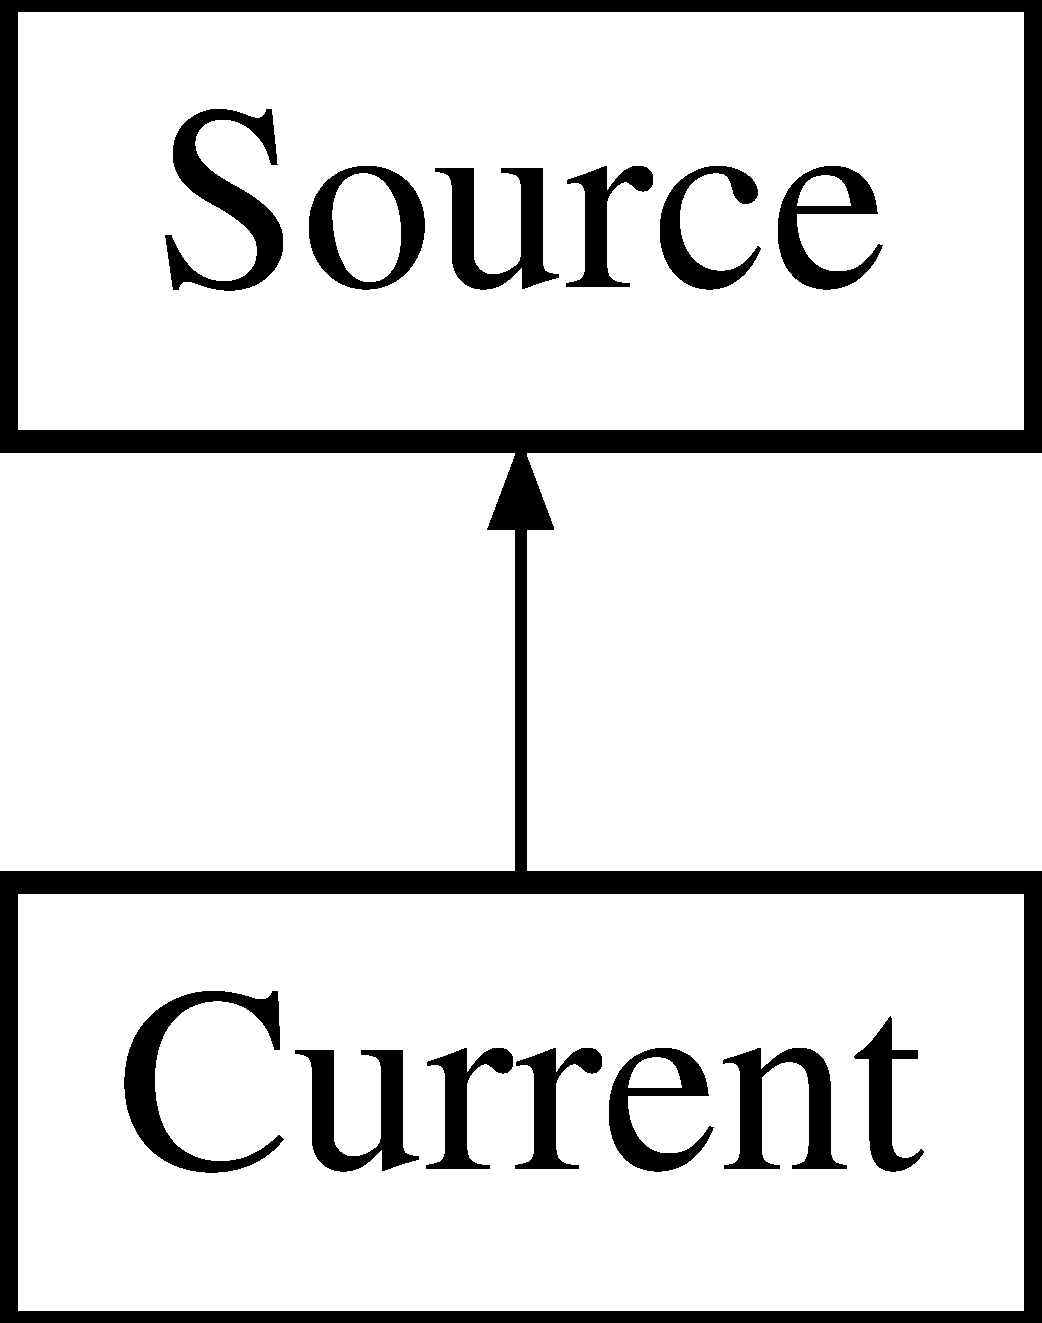
\includegraphics[height=2.000000cm]{class_s_p_i_c_e_1_1_current}
\end{center}
\end{figure}
\subsection*{Public Member Functions}
\begin{DoxyCompactItemize}
\item 
\mbox{\hyperlink{class_s_p_i_c_e_1_1_current_a798deca3f9017adbf1bb2ab5ca2f2f5e}{Current}} (std\+::string name, std\+::string pos, std\+::string neg, std\+::string value)
\begin{DoxyCompactList}\small\item\em creates a new current source. \end{DoxyCompactList}\end{DoxyCompactItemize}
\subsection*{Additional Inherited Members}


\subsection{Detailed Description}
This class describes a current source. 

\subsection{Constructor \& Destructor Documentation}
\mbox{\Hypertarget{class_s_p_i_c_e_1_1_current_a798deca3f9017adbf1bb2ab5ca2f2f5e}\label{class_s_p_i_c_e_1_1_current_a798deca3f9017adbf1bb2ab5ca2f2f5e}} 
\index{S\+P\+I\+C\+E\+::\+Current@{S\+P\+I\+C\+E\+::\+Current}!Current@{Current}}
\index{Current@{Current}!S\+P\+I\+C\+E\+::\+Current@{S\+P\+I\+C\+E\+::\+Current}}
\subsubsection{\texorpdfstring{Current()}{Current()}}
{\footnotesize\ttfamily \mbox{\hyperlink{class_s_p_i_c_e_1_1_current}{Current}} (\begin{DoxyParamCaption}\item[{std\+::string}]{name,  }\item[{std\+::string}]{pos,  }\item[{std\+::string}]{neg,  }\item[{std\+::string}]{value }\end{DoxyParamCaption})\hspace{0.3cm}{\ttfamily [inline]}}



creates a new current source. 


\begin{DoxyParams}{Parameters}
{\em name} & the name of the source. \\
\hline
{\em pos} & the positive connector of the source. \\
\hline
{\em neg} & the negative connector of the source. \\
\hline
{\em value} & the value of the source. \\
\hline
\end{DoxyParams}

\hypertarget{class_open_chams_1_1_d_d_p}{}\section{D\+DP Class Reference}
\label{class_open_chams_1_1_d_d_p}\index{D\+DP@{D\+DP}}
Inheritance diagram for D\+DP\+:\begin{figure}[H]
\begin{center}
\leavevmode
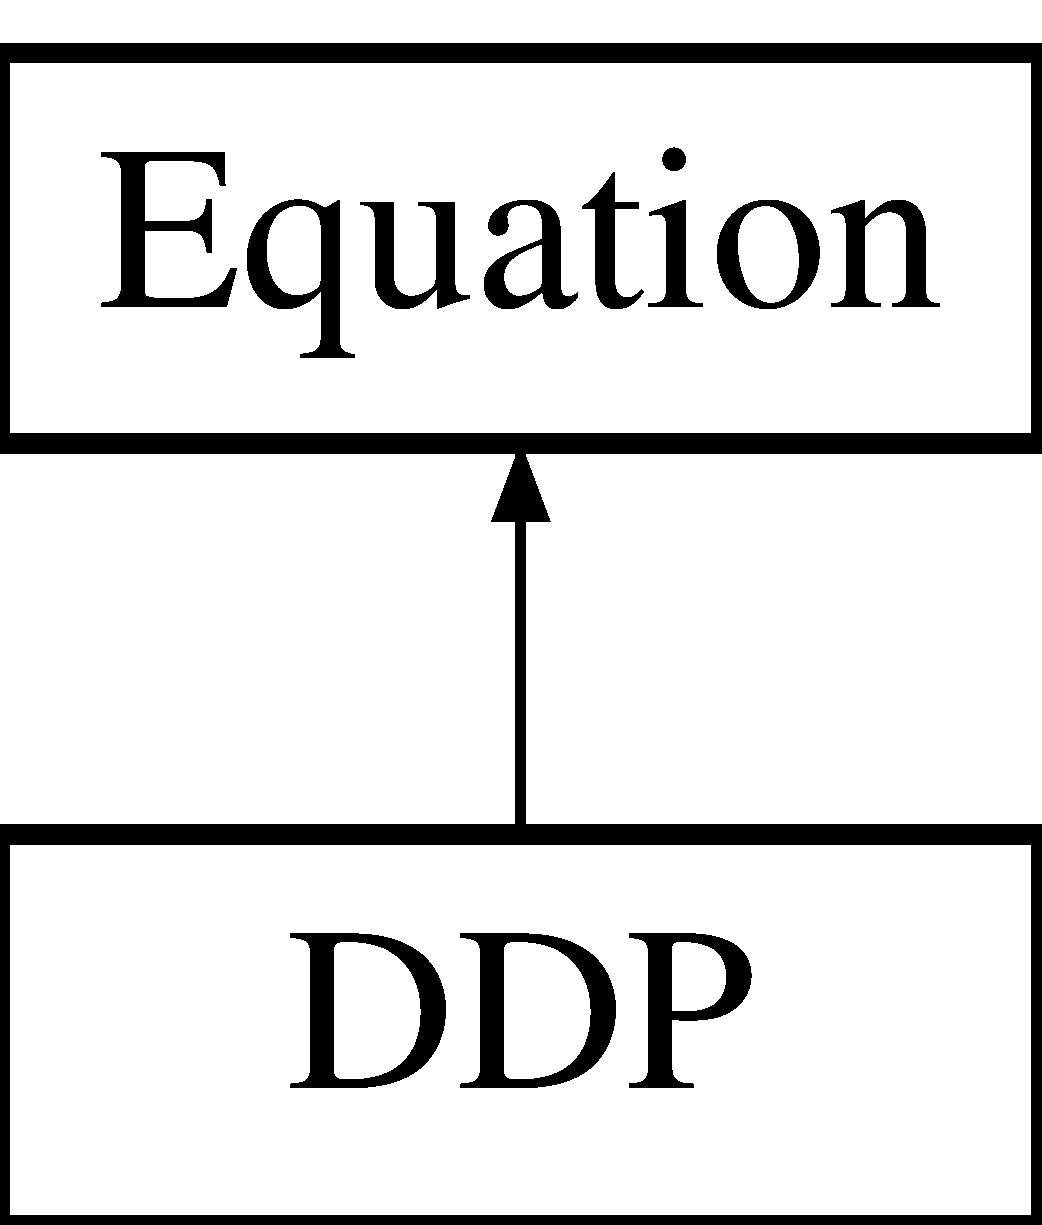
\includegraphics[height=2.000000cm]{class_open_chams_1_1_d_d_p}
\end{center}
\end{figure}

\hypertarget{class_open_chams_1_1_designer_cstr_o_c}{}\section{Designer\+Cstr\+OC Class Reference}
\label{class_open_chams_1_1_designer_cstr_o_c}\index{Designer\+Cstr\+OC@{Designer\+Cstr\+OC}}
Inheritance diagram for Designer\+Cstr\+OC\+:\begin{figure}[H]
\begin{center}
\leavevmode
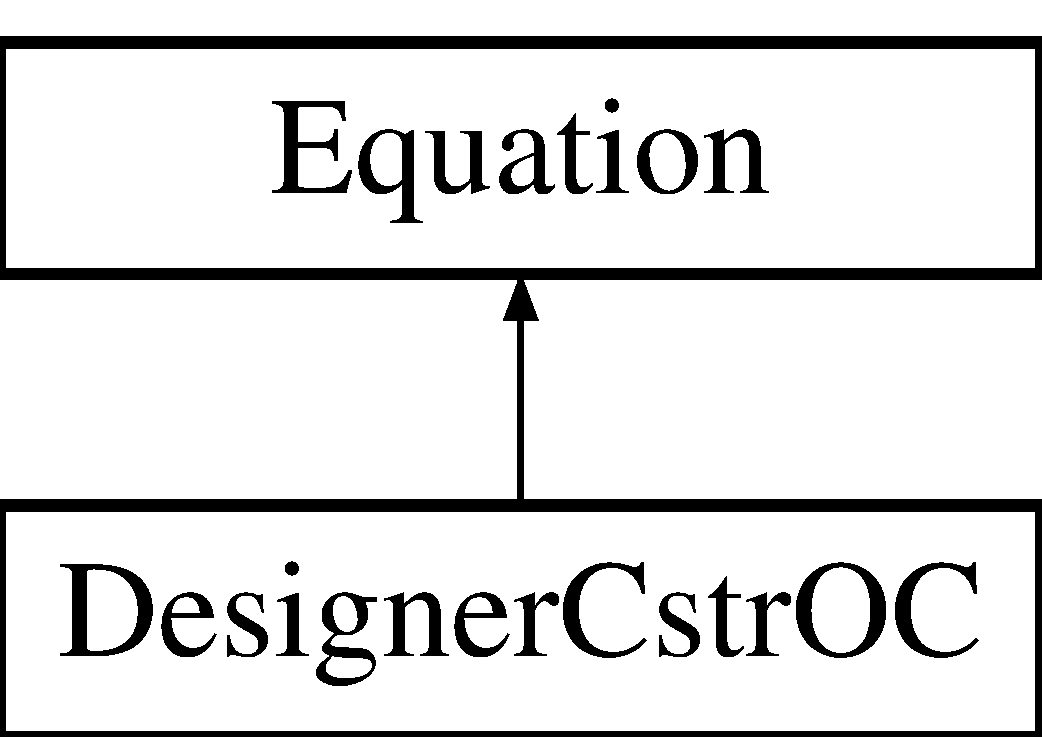
\includegraphics[height=2.000000cm]{class_open_chams_1_1_designer_cstr_o_c}
\end{center}
\end{figure}

\hypertarget{class_open_chams_1_1_device}{}\section{Device Class Reference}
\label{class_open_chams_1_1_device}\index{Device@{Device}}
Inheritance diagram for Device\+:\begin{figure}[H]
\begin{center}
\leavevmode
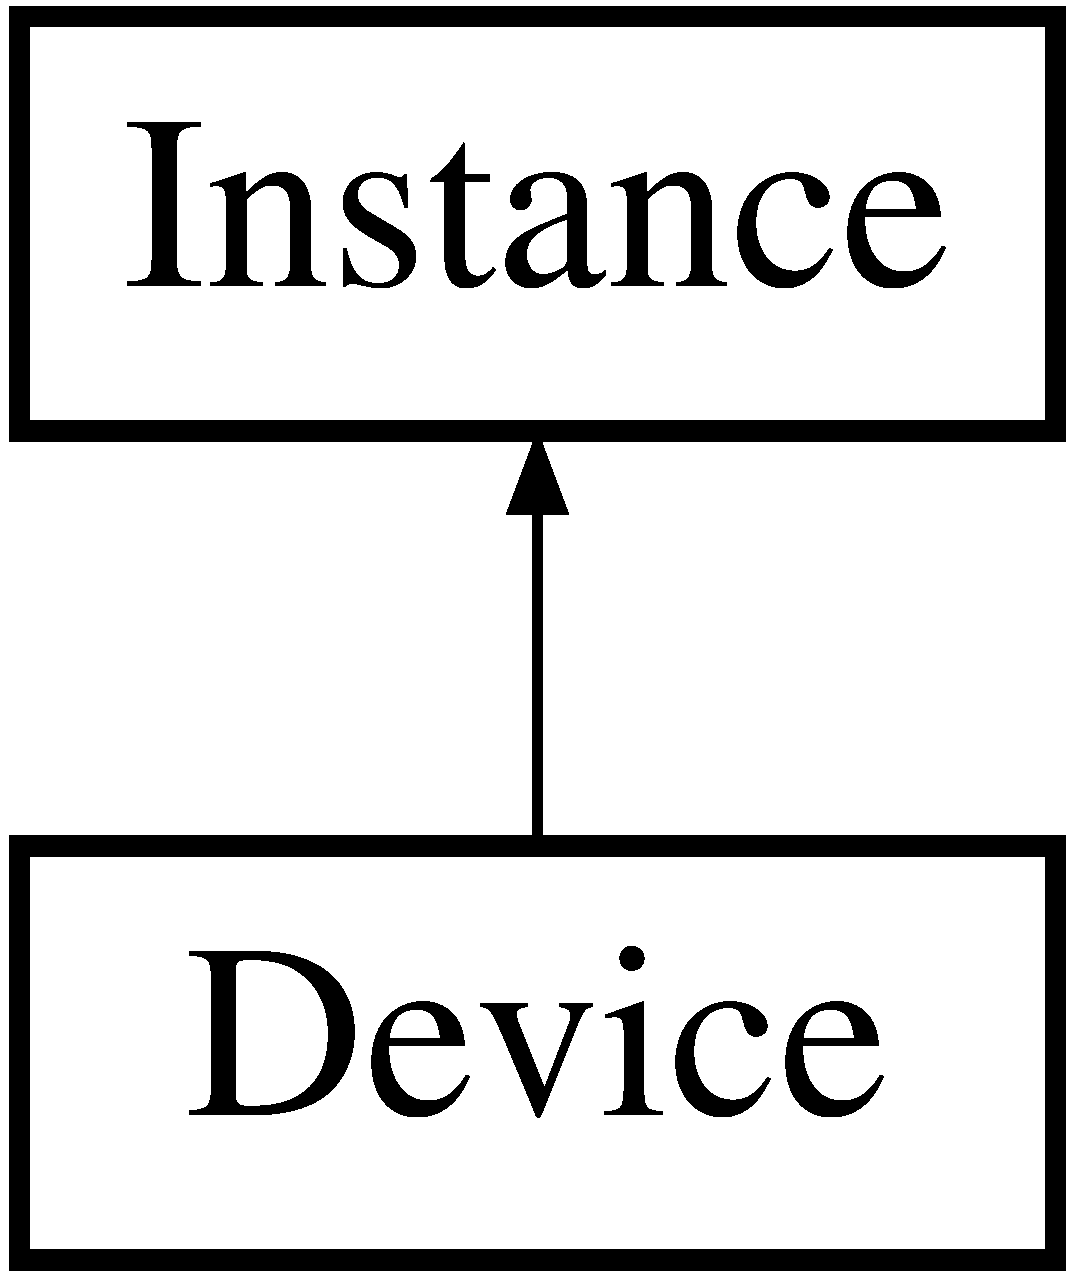
\includegraphics[height=2.000000cm]{class_open_chams_1_1_device}
\end{center}
\end{figure}
\subsection*{Public Member Functions}
\begin{DoxyCompactItemize}
\item 
\mbox{\hyperlink{class_open_chams_1_1_transistor}{Transistor}} $\ast$ \mbox{\hyperlink{class_open_chams_1_1_device_ad45d34f8765dd113a5b12289efe66c07}{add\+Transistor}} (const std\+::string \&)
\begin{DoxyCompactList}\small\item\em adds a \mbox{\hyperlink{class_open_chams_1_1_transistor}{Transistor}} to the device. \end{DoxyCompactList}\item 
\mbox{\hyperlink{class_open_chams_1_1_device_af5d1871d38a605955d7848d07df6d9a4}{Device}} (const std\+::string \&name, const std\+::string \&model, unsigned order, const std\+::string \&mos\+Type, bool source\+Bulk\+Connected, \mbox{\hyperlink{class_open_chams_1_1_netlist}{Netlist}} $\ast$)
\begin{DoxyCompactList}\small\item\em creates a new device. \end{DoxyCompactList}\item 
\mbox{\Hypertarget{class_open_chams_1_1_device_a831ce553c23908f447a5be332ecd5946}\label{class_open_chams_1_1_device_a831ce553c23908f447a5be332ecd5946}} 
const std\+::string \& \mbox{\hyperlink{class_open_chams_1_1_device_a831ce553c23908f447a5be332ecd5946}{get\+Mos\+Type}} ()
\begin{DoxyCompactList}\small\item\em returns the mos type of the device. \end{DoxyCompactList}\item 
\mbox{\Hypertarget{class_open_chams_1_1_device_a4033525cab6387eb057f71f5feed9802}\label{class_open_chams_1_1_device_a4033525cab6387eb057f71f5feed9802}} 
const std\+::vector$<$ \mbox{\hyperlink{class_open_chams_1_1_transistor}{Transistor}} $\ast$ $>$ \& \mbox{\hyperlink{class_open_chams_1_1_device_a4033525cab6387eb057f71f5feed9802}{get\+Transistors}} ()
\begin{DoxyCompactList}\small\item\em returns the list of device\textquotesingle{}s transistors. \end{DoxyCompactList}\item 
\mbox{\Hypertarget{class_open_chams_1_1_device_aa9d93f306256ac57b8bb8a4cb436c8d3}\label{class_open_chams_1_1_device_aa9d93f306256ac57b8bb8a4cb436c8d3}} 
bool \mbox{\hyperlink{class_open_chams_1_1_device_aa9d93f306256ac57b8bb8a4cb436c8d3}{has\+No\+Transistors}} ()
\begin{DoxyCompactList}\small\item\em returns true if the device has no transistors. \end{DoxyCompactList}\item 
\mbox{\Hypertarget{class_open_chams_1_1_device_a29ed1982e1a8b3a634df8d0c70039669}\label{class_open_chams_1_1_device_a29ed1982e1a8b3a634df8d0c70039669}} 
bool \mbox{\hyperlink{class_open_chams_1_1_device_a29ed1982e1a8b3a634df8d0c70039669}{is\+Source\+Bulk\+Connected}} ()
\begin{DoxyCompactList}\small\item\em returns true if the device\textquotesingle{}s bulk is source connected. \end{DoxyCompactList}\end{DoxyCompactItemize}


\subsection{Detailed Description}
This class describes a \mbox{\hyperlink{class_open_chams_1_1_device}{Device}}.

A device is a leaf instance which means its model is not defined in a external file but is described inside the device. As an instance, the \mbox{\hyperlink{class_open_chams_1_1_device}{Device}} inherits all \mbox{\hyperlink{class_open_chams_1_1_instance}{Instance}} methods and adds specific properties\+: mos type, bulk connection and list of internal transistors.

\begin{DoxyNote}{Note}
Althought today \mbox{\hyperlink{class_open_chams_1_1_device}{Device}} object only consider Transistor\+Family devices, it will have to consider other devices, such as Capacitor when C\+H\+A\+MS project will. 
\end{DoxyNote}


\subsection{Constructor \& Destructor Documentation}
\mbox{\Hypertarget{class_open_chams_1_1_device_af5d1871d38a605955d7848d07df6d9a4}\label{class_open_chams_1_1_device_af5d1871d38a605955d7848d07df6d9a4}} 
\index{Open\+Chams\+::\+Device@{Open\+Chams\+::\+Device}!Device@{Device}}
\index{Device@{Device}!Open\+Chams\+::\+Device@{Open\+Chams\+::\+Device}}
\subsubsection{\texorpdfstring{Device()}{Device()}}
{\footnotesize\ttfamily \mbox{\hyperlink{class_open_chams_1_1_device}{Device}} (\begin{DoxyParamCaption}\item[{const std\+::string \&}]{name,  }\item[{const std\+::string \&}]{model,  }\item[{unsigned}]{order,  }\item[{const std\+::string \&}]{mos\+Type,  }\item[{bool}]{source\+Bulk\+Connected,  }\item[{\mbox{\hyperlink{class_open_chams_1_1_netlist}{Netlist}} $\ast$}]{netlist }\end{DoxyParamCaption})}



creates a new device. 


\begin{DoxyParams}{Parameters}
{\em name} & the name of the instance. \\
\hline
{\em model} & the model of the instance. \\
\hline
{\em mos\+Type} & the mos type (N\+M\+OS or P\+M\+OS). \\
\hline
{\em netlist} & the netlist to which the instance belongs. \\
\hline
\end{DoxyParams}


\subsection{Member Function Documentation}
\mbox{\Hypertarget{class_open_chams_1_1_device_ad45d34f8765dd113a5b12289efe66c07}\label{class_open_chams_1_1_device_ad45d34f8765dd113a5b12289efe66c07}} 
\index{Open\+Chams\+::\+Device@{Open\+Chams\+::\+Device}!add\+Transistor@{add\+Transistor}}
\index{add\+Transistor@{add\+Transistor}!Open\+Chams\+::\+Device@{Open\+Chams\+::\+Device}}
\subsubsection{\texorpdfstring{add\+Transistor()}{addTransistor()}}
{\footnotesize\ttfamily \mbox{\hyperlink{class_open_chams_1_1_transistor}{Transistor}} $\ast$ add\+Transistor (\begin{DoxyParamCaption}\item[{const std\+::string \&}]{name }\end{DoxyParamCaption})}



adds a \mbox{\hyperlink{class_open_chams_1_1_transistor}{Transistor}} to the device. 


\begin{DoxyParams}{Parameters}
{\em name} & the name of the transistor.\\
\hline
\end{DoxyParams}
\begin{DoxyReturn}{Returns}
the newly created \mbox{\hyperlink{class_open_chams_1_1_transistor}{Transistor}}. 
\end{DoxyReturn}

\hypertarget{class_open_chams_1_1_d_slicing_node}{\section{D\-Slicing\-Node Class Reference}
\label{class_open_chams_1_1_d_slicing_node}\index{D\-Slicing\-Node@{D\-Slicing\-Node}}
}
Inheritance diagram for D\-Slicing\-Node\-:\begin{figure}[H]
\begin{center}
\leavevmode
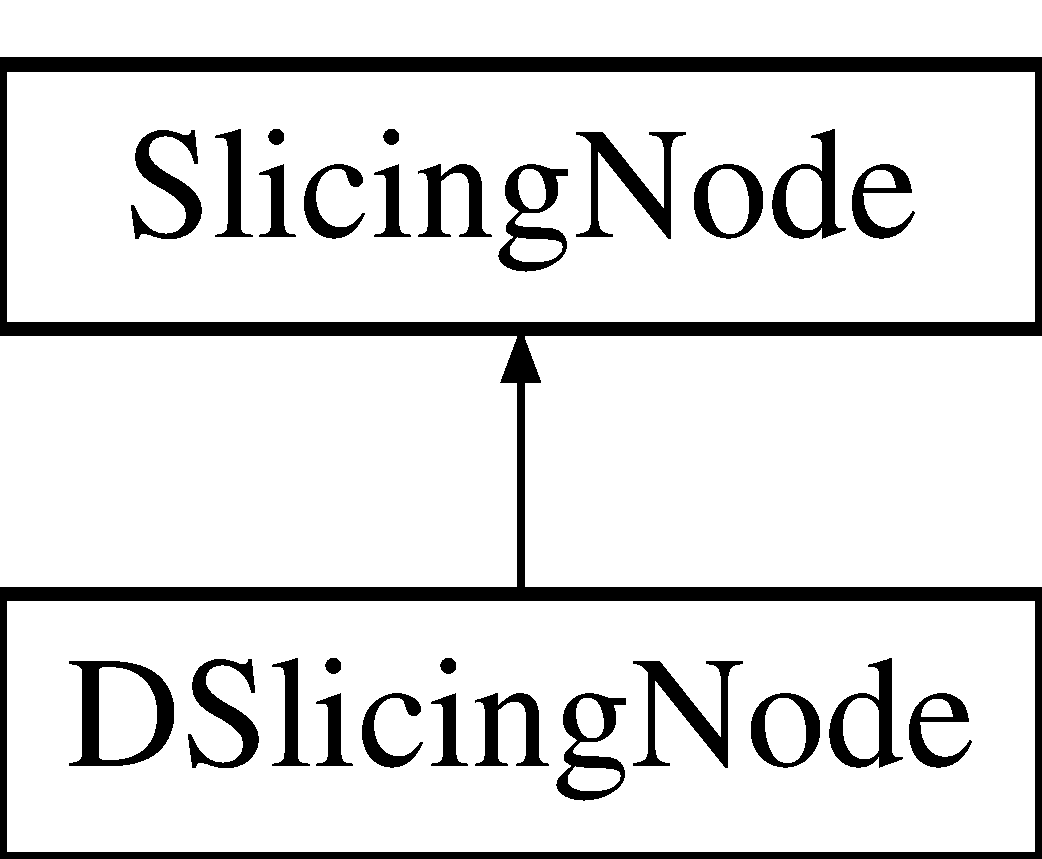
\includegraphics[height=2.000000cm]{class_open_chams_1_1_d_slicing_node}
\end{center}
\end{figure}

\hypertarget{class_d_t_r_1_1_d_t_r_exception}{}\section{D\+T\+R\+Exception Class Reference}
\label{class_d_t_r_1_1_d_t_r_exception}\index{D\+T\+R\+Exception@{D\+T\+R\+Exception}}


\subsection{Detailed Description}
This class describes the exceptions throwed by the D\+TR library in case of errors. 
\hypertarget{class_a_g_d_s_1_1_element}{}\section{Element Class Reference}
\label{class_a_g_d_s_1_1_element}\index{Element@{Element}}
Inheritance diagram for Element\+:\begin{figure}[H]
\begin{center}
\leavevmode
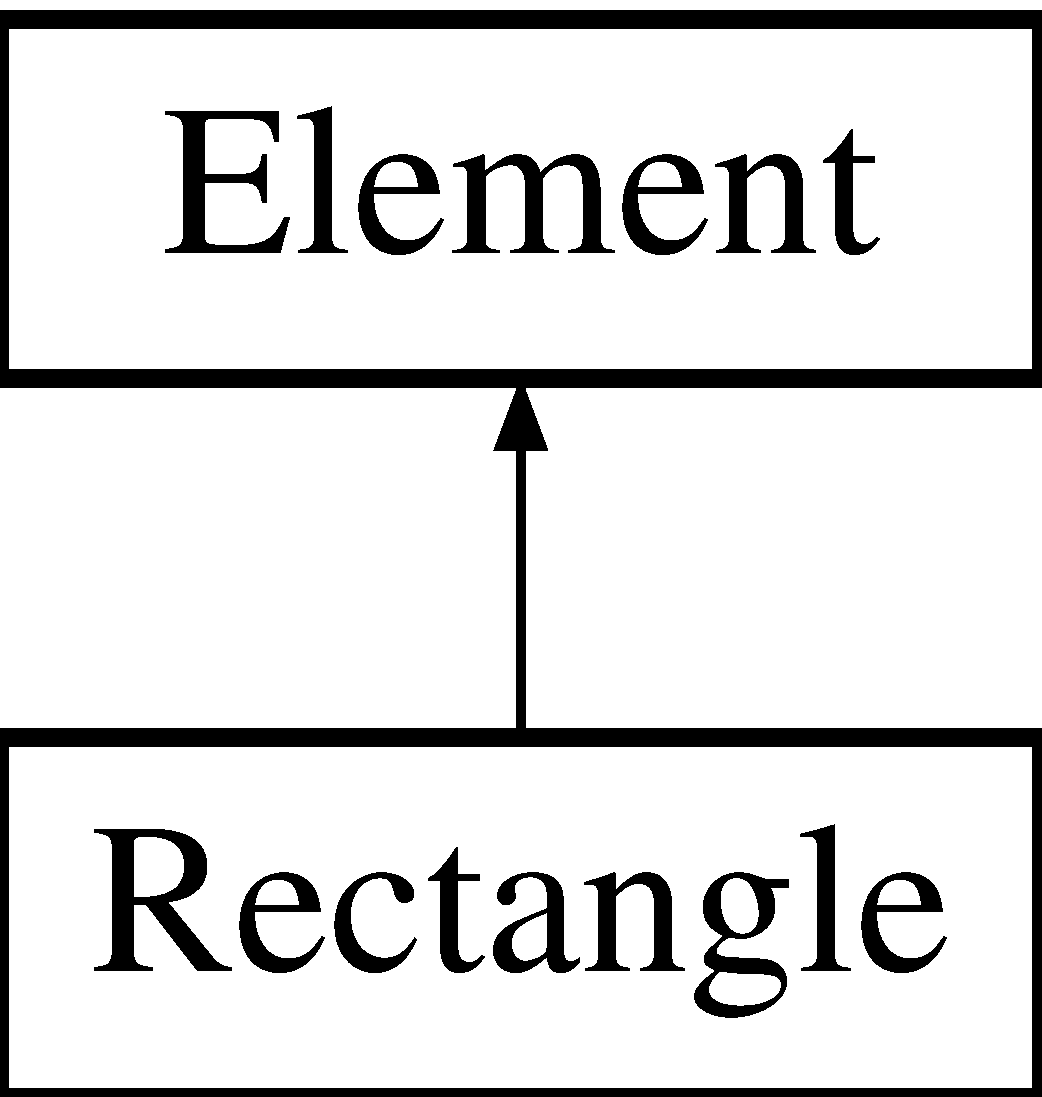
\includegraphics[height=2.000000cm]{class_a_g_d_s_1_1_element}
\end{center}
\end{figure}


\subsection{Detailed Description}
This is an abstract class which is a base for any G\+DS II shape. It only defines a layer. 
\hypertarget{class_open_chams_1_1_equation}{\section{Equation Class Reference}
\label{class_open_chams_1_1_equation}\index{Equation@{Equation}}
}
Inheritance diagram for Equation\-:\begin{figure}[H]
\begin{center}
\leavevmode
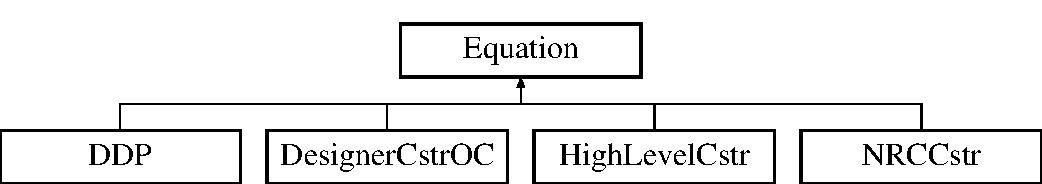
\includegraphics[height=2.000000cm]{class_open_chams_1_1_equation}
\end{center}
\end{figure}

\hypertarget{class_open_chams_1_1_group}{}\section{Group Class Reference}
\label{class_open_chams_1_1_group}\index{Group@{Group}}
Inheritance diagram for Group\+:\begin{figure}[H]
\begin{center}
\leavevmode
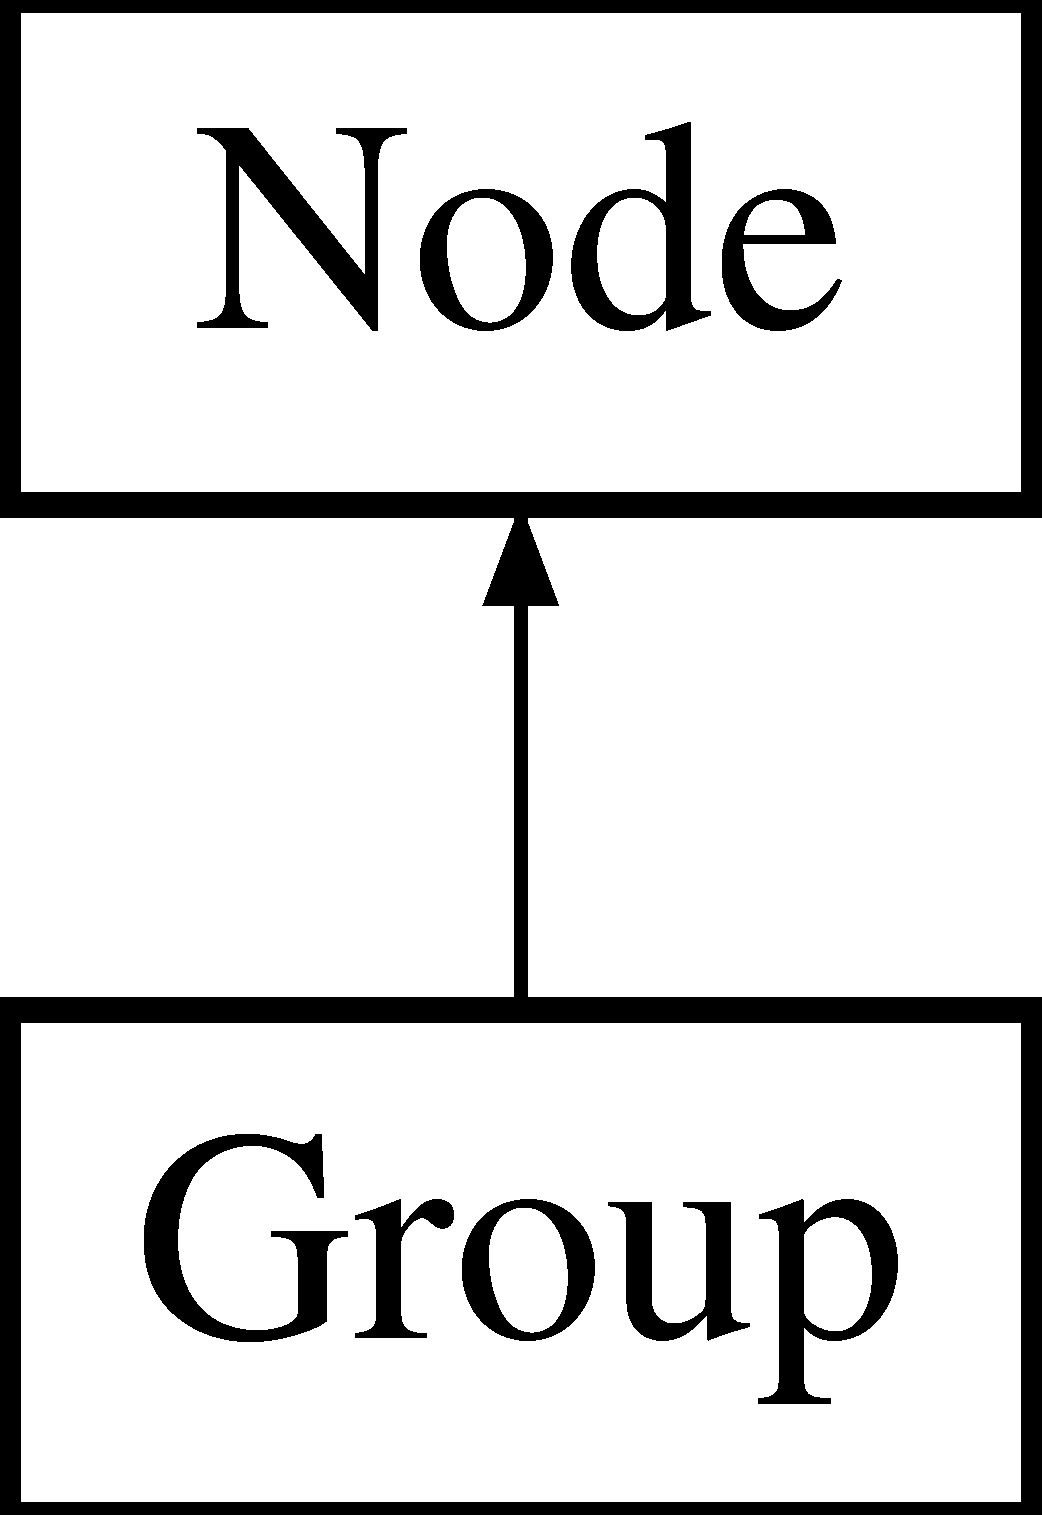
\includegraphics[height=2.000000cm]{class_open_chams_1_1_group}
\end{center}
\end{figure}
\subsection*{Public Member Functions}
\begin{DoxyCompactItemize}
\item 
\mbox{\Hypertarget{class_open_chams_1_1_group_a7cff0c4a6957f23fb1ea4598f4b8a0b8}\label{class_open_chams_1_1_group_a7cff0c4a6957f23fb1ea4598f4b8a0b8}} 
Align \mbox{\hyperlink{class_open_chams_1_1_group_a7cff0c4a6957f23fb1ea4598f4b8a0b8}{get\+Align}} ()
\begin{DoxyCompactList}\small\item\em returns the alignment constraint of the group. \end{DoxyCompactList}\item 
\mbox{\Hypertarget{class_open_chams_1_1_group_ab5ae4a4550c418c974ff6e59967eeec2}\label{class_open_chams_1_1_group_ab5ae4a4550c418c974ff6e59967eeec2}} 
bool \mbox{\hyperlink{class_open_chams_1_1_group_ab5ae4a4550c418c974ff6e59967eeec2}{is\+Isolated}} ()
\begin{DoxyCompactList}\small\item\em returns true if the group has an isolation constraint. \end{DoxyCompactList}\item 
\mbox{\Hypertarget{class_open_chams_1_1_group_aee0abf07a6e9d41f511c648e6eaecea3}\label{class_open_chams_1_1_group_aee0abf07a6e9d41f511c648e6eaecea3}} 
bool \mbox{\hyperlink{class_open_chams_1_1_group_aee0abf07a6e9d41f511c648e6eaecea3}{is\+Paired}} ()
\begin{DoxyCompactList}\small\item\em returns true if the group has a pairing constraint. \end{DoxyCompactList}\item 
void \mbox{\hyperlink{class_open_chams_1_1_group_a9fc27b2bc4da99c723102153c4fbf1c0}{set\+Align}} (Align)
\begin{DoxyCompactList}\small\item\em sets an alignment constraint on the group. \end{DoxyCompactList}\item 
void \mbox{\hyperlink{class_open_chams_1_1_group_abefcd8ede34b508fe7d42428a618cb02}{set\+Isolated}} (bool)
\begin{DoxyCompactList}\small\item\em sets whether the group has an isolation constraint or not. \end{DoxyCompactList}\item 
void \mbox{\hyperlink{class_open_chams_1_1_group_aff6de4e5c0da79ad8d0070c03bfd941b}{set\+Paired}} (bool)
\begin{DoxyCompactList}\small\item\em sets whether the group has a pairing constraint or not. \end{DoxyCompactList}\item 
void \mbox{\hyperlink{class_open_chams_1_1_group_adc93b900e943312e905182fe44f21225}{set\+Root\+Node}} (\mbox{\hyperlink{class_open_chams_1_1_node}{Node}} $\ast$)
\begin{DoxyCompactList}\small\item\em sets the root node of the group. \end{DoxyCompactList}\end{DoxyCompactItemize}


\subsection{Detailed Description}
This class describes a group of the placement tree. 

\subsection{Member Function Documentation}
\mbox{\Hypertarget{class_open_chams_1_1_group_a9fc27b2bc4da99c723102153c4fbf1c0}\label{class_open_chams_1_1_group_a9fc27b2bc4da99c723102153c4fbf1c0}} 
\index{Open\+Chams\+::\+Group@{Open\+Chams\+::\+Group}!set\+Align@{set\+Align}}
\index{set\+Align@{set\+Align}!Open\+Chams\+::\+Group@{Open\+Chams\+::\+Group}}
\subsubsection{\texorpdfstring{set\+Align()}{setAlign()}}
{\footnotesize\ttfamily void set\+Align (\begin{DoxyParamCaption}\item[{Group\+::\+Align}]{align }\end{DoxyParamCaption})\hspace{0.3cm}{\ttfamily [inline]}}



sets an alignment constraint on the group. 


\begin{DoxyParams}{Parameters}
{\em align} & the value of the alignment constraint can be N\+O\+NE, V\+E\+R\+T\+I\+C\+AL or H\+O\+R\+I\+Z\+O\+N\+T\+AL. \\
\hline
\end{DoxyParams}
\mbox{\Hypertarget{class_open_chams_1_1_group_abefcd8ede34b508fe7d42428a618cb02}\label{class_open_chams_1_1_group_abefcd8ede34b508fe7d42428a618cb02}} 
\index{Open\+Chams\+::\+Group@{Open\+Chams\+::\+Group}!set\+Isolated@{set\+Isolated}}
\index{set\+Isolated@{set\+Isolated}!Open\+Chams\+::\+Group@{Open\+Chams\+::\+Group}}
\subsubsection{\texorpdfstring{set\+Isolated()}{setIsolated()}}
{\footnotesize\ttfamily void set\+Isolated (\begin{DoxyParamCaption}\item[{bool}]{isolated }\end{DoxyParamCaption})\hspace{0.3cm}{\ttfamily [inline]}}



sets whether the group has an isolation constraint or not. 


\begin{DoxyParams}{Parameters}
{\em isolated} & if true the group has an isolation constraint. \\
\hline
\end{DoxyParams}
\mbox{\Hypertarget{class_open_chams_1_1_group_aff6de4e5c0da79ad8d0070c03bfd941b}\label{class_open_chams_1_1_group_aff6de4e5c0da79ad8d0070c03bfd941b}} 
\index{Open\+Chams\+::\+Group@{Open\+Chams\+::\+Group}!set\+Paired@{set\+Paired}}
\index{set\+Paired@{set\+Paired}!Open\+Chams\+::\+Group@{Open\+Chams\+::\+Group}}
\subsubsection{\texorpdfstring{set\+Paired()}{setPaired()}}
{\footnotesize\ttfamily void set\+Paired (\begin{DoxyParamCaption}\item[{bool}]{paired }\end{DoxyParamCaption})\hspace{0.3cm}{\ttfamily [inline]}}



sets whether the group has a pairing constraint or not. 


\begin{DoxyParams}{Parameters}
{\em paired} & if true the group has a pairing constraint. \\
\hline
\end{DoxyParams}
\mbox{\Hypertarget{class_open_chams_1_1_group_adc93b900e943312e905182fe44f21225}\label{class_open_chams_1_1_group_adc93b900e943312e905182fe44f21225}} 
\index{Open\+Chams\+::\+Group@{Open\+Chams\+::\+Group}!set\+Root\+Node@{set\+Root\+Node}}
\index{set\+Root\+Node@{set\+Root\+Node}!Open\+Chams\+::\+Group@{Open\+Chams\+::\+Group}}
\subsubsection{\texorpdfstring{set\+Root\+Node()}{setRootNode()}}
{\footnotesize\ttfamily void set\+Root\+Node (\begin{DoxyParamCaption}\item[{\mbox{\hyperlink{class_open_chams_1_1_node}{Node}} $\ast$}]{node }\end{DoxyParamCaption})\hspace{0.3cm}{\ttfamily [inline]}}



sets the root node of the group. 


\begin{DoxyParams}{Parameters}
{\em node} & the root node of the group \\
\hline
\end{DoxyParams}

\hypertarget{class_open_chams_1_1_high_level_cstr}{\section{High\-Level\-Cstr Class Reference}
\label{class_open_chams_1_1_high_level_cstr}\index{High\-Level\-Cstr@{High\-Level\-Cstr}}
}
Inheritance diagram for High\-Level\-Cstr\-:\begin{figure}[H]
\begin{center}
\leavevmode
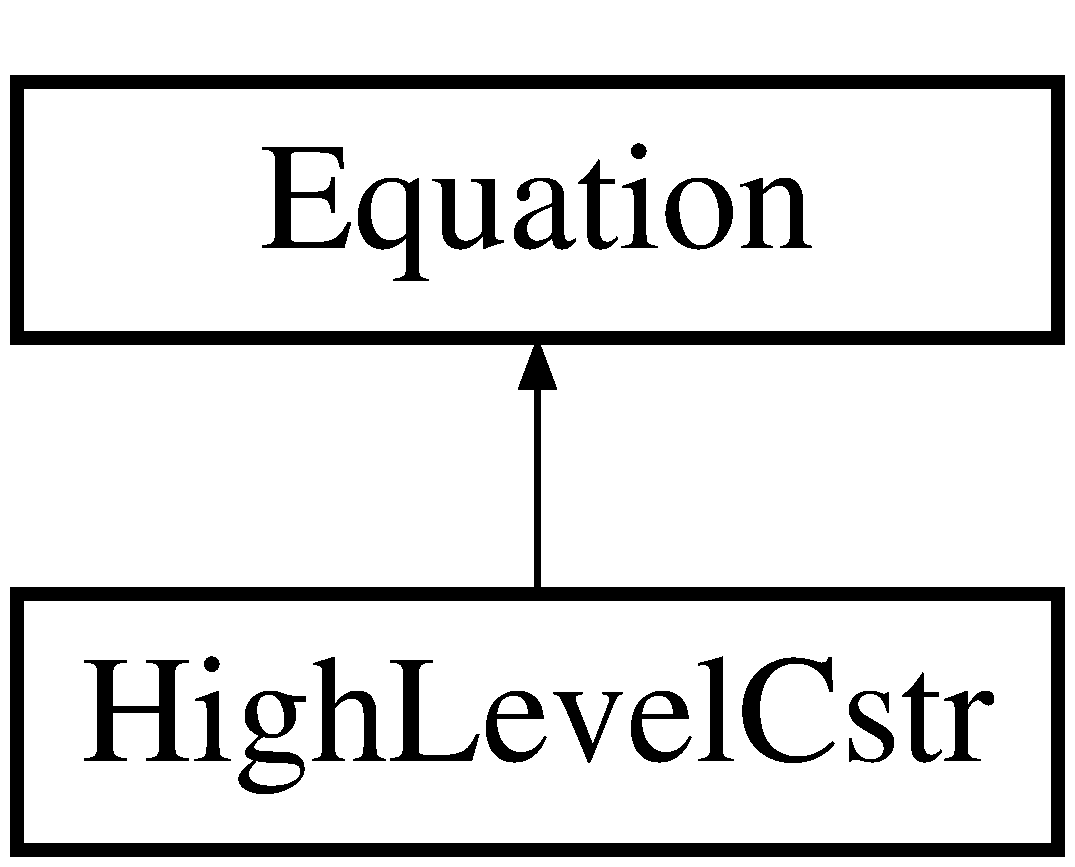
\includegraphics[height=2.000000cm]{class_open_chams_1_1_high_level_cstr}
\end{center}
\end{figure}

\hypertarget{class_open_chams_1_1_h_slicing_node}{\section{H\-Slicing\-Node Class Reference}
\label{class_open_chams_1_1_h_slicing_node}\index{H\-Slicing\-Node@{H\-Slicing\-Node}}
}
Inheritance diagram for H\-Slicing\-Node\-:\begin{figure}[H]
\begin{center}
\leavevmode
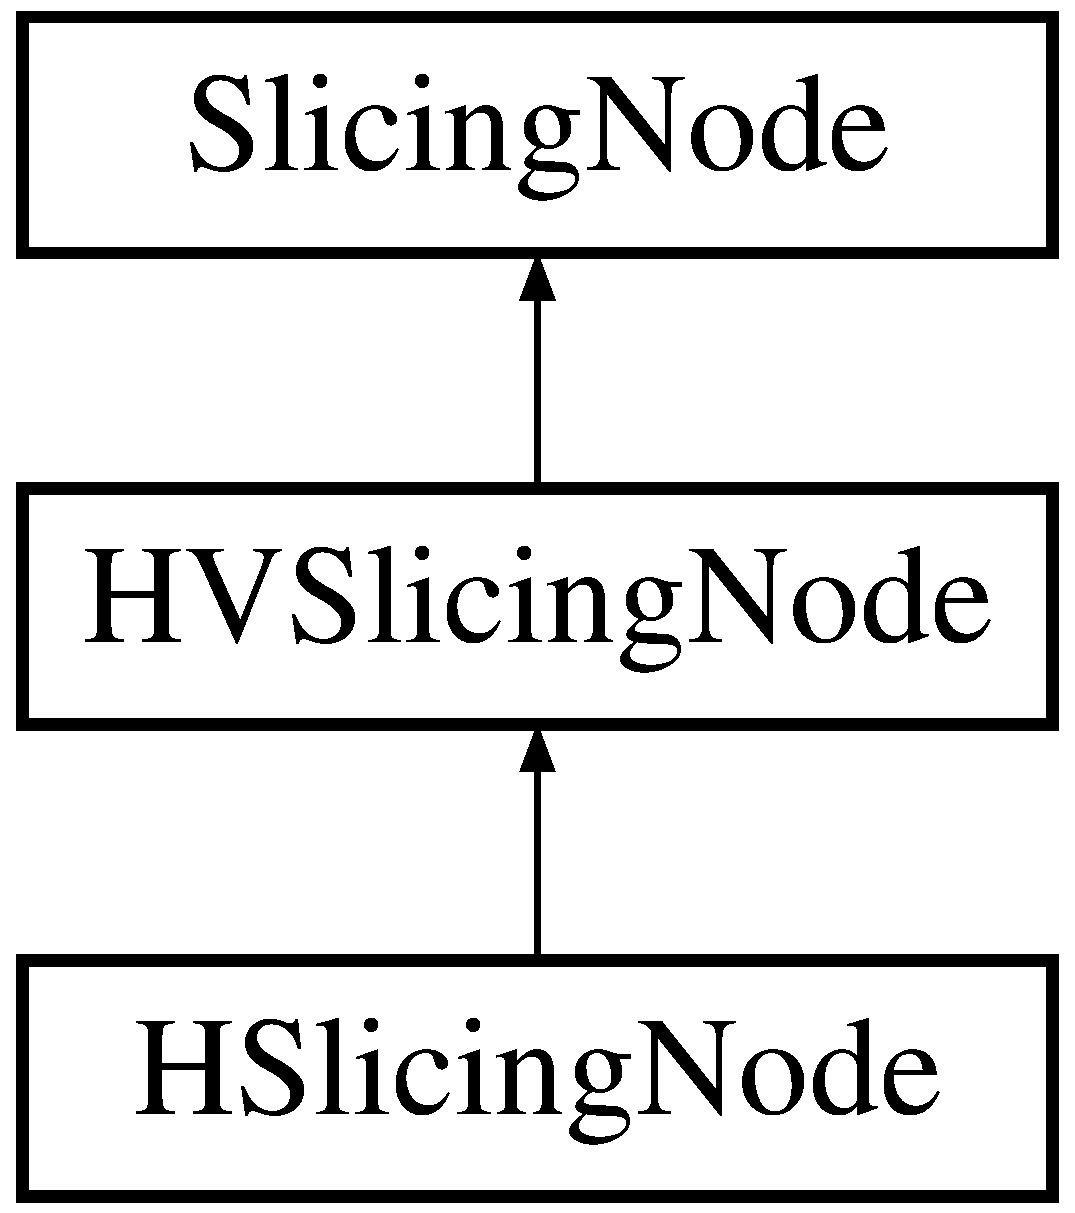
\includegraphics[height=3.000000cm]{class_open_chams_1_1_h_slicing_node}
\end{center}
\end{figure}

\hypertarget{class_open_chams_1_1_h_v_slicing_node}{}\section{H\+V\+Slicing\+Node Class Reference}
\label{class_open_chams_1_1_h_v_slicing_node}\index{H\+V\+Slicing\+Node@{H\+V\+Slicing\+Node}}
Inheritance diagram for H\+V\+Slicing\+Node\+:\begin{figure}[H]
\begin{center}
\leavevmode
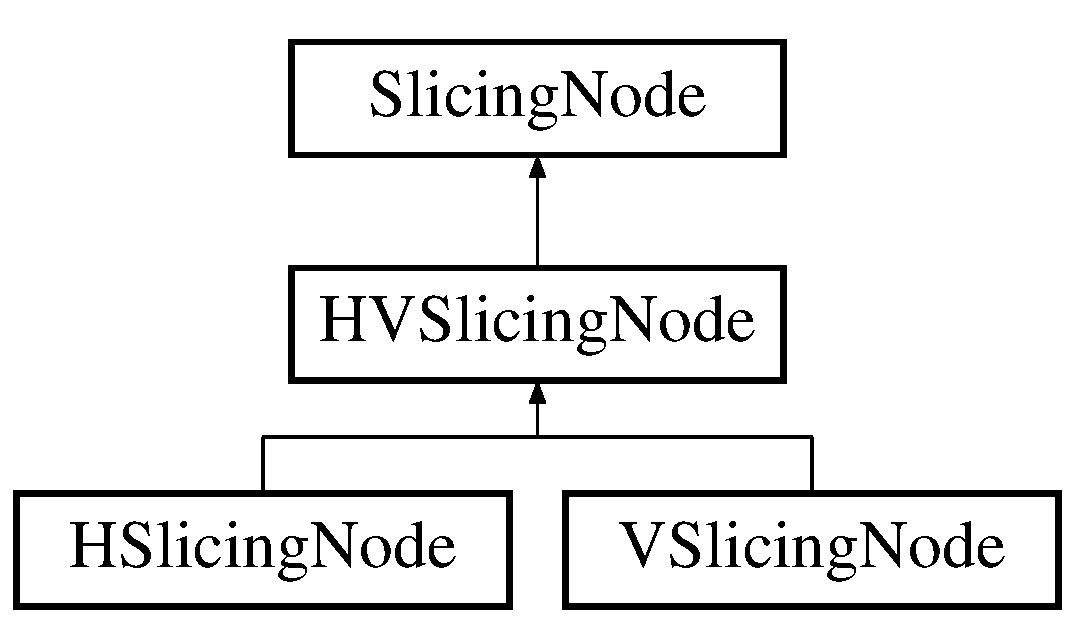
\includegraphics[height=3.000000cm]{class_open_chams_1_1_h_v_slicing_node}
\end{center}
\end{figure}

\hypertarget{class_open_chams_1_1_schematic_1_1_infos}{}\section{Schematic\+:\+:Infos Class Reference}
\label{class_open_chams_1_1_schematic_1_1_infos}\index{Schematic\+::\+Infos@{Schematic\+::\+Infos}}
\subsection*{Public Member Functions}
\begin{DoxyCompactItemize}
\item 
\mbox{\Hypertarget{class_open_chams_1_1_schematic_1_1_infos_ac7e0f89be2baffb526b2dca46da7aa47}\label{class_open_chams_1_1_schematic_1_1_infos_ac7e0f89be2baffb526b2dca46da7aa47}} 
const std\+::string \& \hyperlink{class_open_chams_1_1_schematic_1_1_infos_ac7e0f89be2baffb526b2dca46da7aa47}{get\+Orientation} ()
\begin{DoxyCompactList}\small\item\em returns the orientation. \end{DoxyCompactList}\item 
\mbox{\Hypertarget{class_open_chams_1_1_schematic_1_1_infos_a2b69e4312b7814c6efce42f851893409}\label{class_open_chams_1_1_schematic_1_1_infos_a2b69e4312b7814c6efce42f851893409}} 
double \hyperlink{class_open_chams_1_1_schematic_1_1_infos_a2b69e4312b7814c6efce42f851893409}{getX} ()
\begin{DoxyCompactList}\small\item\em returns the x coordinate. \end{DoxyCompactList}\item 
\mbox{\Hypertarget{class_open_chams_1_1_schematic_1_1_infos_a15f19cf52955c8c3406831b288681358}\label{class_open_chams_1_1_schematic_1_1_infos_a15f19cf52955c8c3406831b288681358}} 
double \hyperlink{class_open_chams_1_1_schematic_1_1_infos_a15f19cf52955c8c3406831b288681358}{getY} ()
\begin{DoxyCompactList}\small\item\em returns the y coordinate. \end{DoxyCompactList}\item 
\hyperlink{class_open_chams_1_1_schematic_1_1_infos_a90e945d2bd4aa8a4f1488fc1466207cb}{Infos} (double x, double y, const std\+::string \&orient)
\begin{DoxyCompactList}\small\item\em creates a new \hyperlink{class_open_chams_1_1_schematic_1_1_infos}{Infos} object. \end{DoxyCompactList}\end{DoxyCompactItemize}


\subsection{Detailed Description}
This class describes schematic informations for an instance. It contains x and y coordinates and the orientation of the instance. 

\subsection{Constructor \& Destructor Documentation}
\mbox{\Hypertarget{class_open_chams_1_1_schematic_1_1_infos_a90e945d2bd4aa8a4f1488fc1466207cb}\label{class_open_chams_1_1_schematic_1_1_infos_a90e945d2bd4aa8a4f1488fc1466207cb}} 
\index{Open\+Chams\+::\+Schematic\+::\+Infos@{Open\+Chams\+::\+Schematic\+::\+Infos}!Infos@{Infos}}
\index{Infos@{Infos}!Open\+Chams\+::\+Schematic\+::\+Infos@{Open\+Chams\+::\+Schematic\+::\+Infos}}
\subsubsection{\texorpdfstring{Infos()}{Infos()}}
{\footnotesize\ttfamily \hyperlink{class_open_chams_1_1_schematic_1_1_infos}{Infos} (\begin{DoxyParamCaption}\item[{double}]{x,  }\item[{double}]{y,  }\item[{const std\+::string \&}]{orient }\end{DoxyParamCaption})}



creates a new \hyperlink{class_open_chams_1_1_schematic_1_1_infos}{Infos} object. 


\begin{DoxyParams}{Parameters}
{\em x} & the x coordinate. \\
\hline
{\em y} & the y corrdinate. \\
\hline
{\em orient} & the orientation. \\
\hline
\end{DoxyParams}

\hypertarget{class_open_chams_1_1_instance}{\section{Instance Class Reference}
\label{class_open_chams_1_1_instance}\index{Instance@{Instance}}
}
Inheritance diagram for Instance\-:\begin{figure}[H]
\begin{center}
\leavevmode
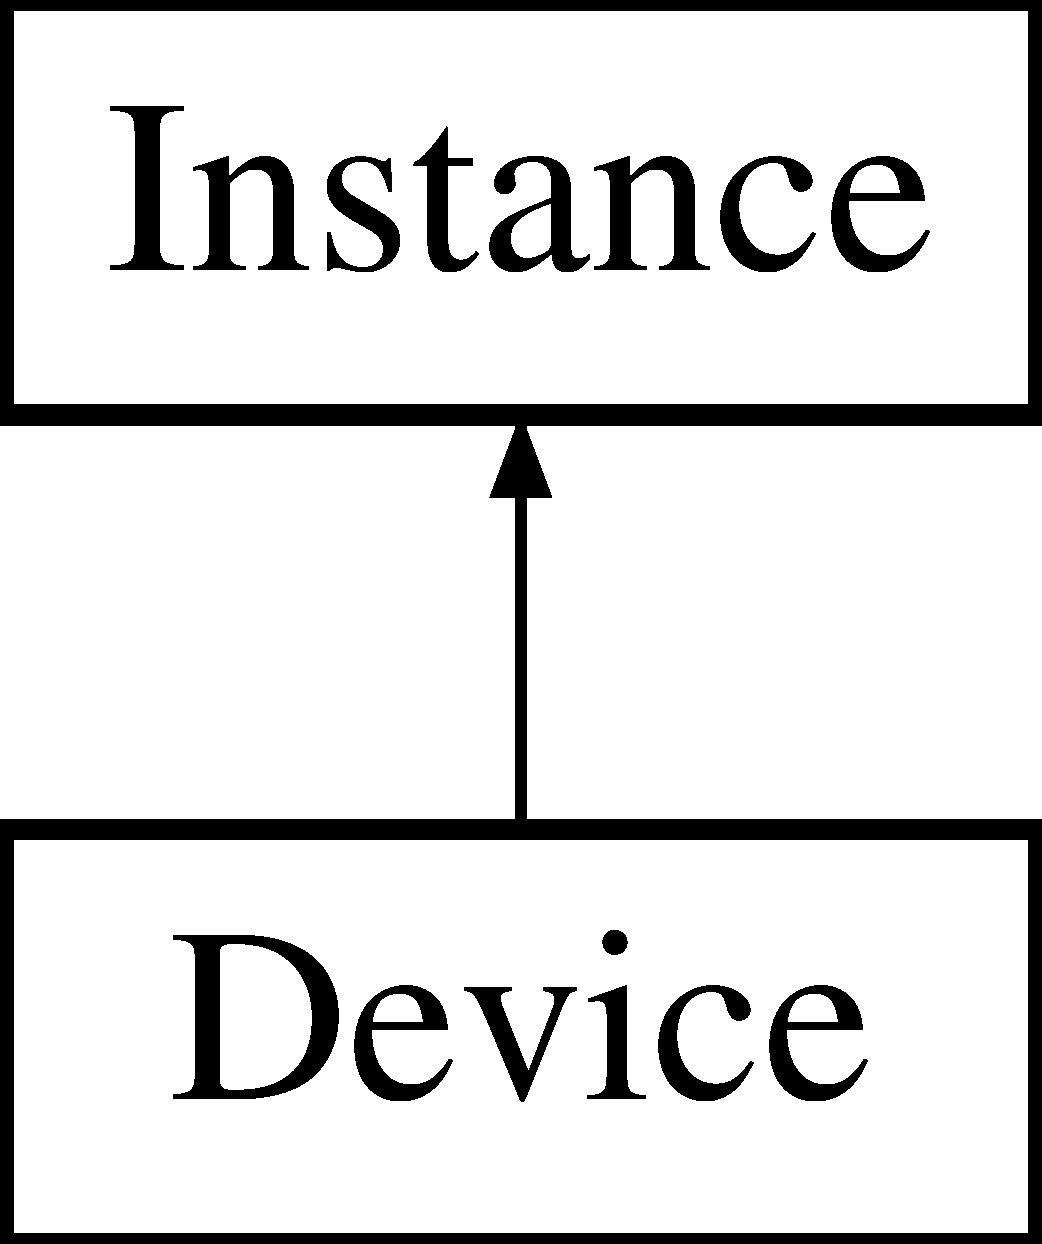
\includegraphics[height=2.000000cm]{class_open_chams_1_1_instance}
\end{center}
\end{figure}
\subsection*{Public Member Functions}
\begin{DoxyCompactItemize}
\item 
void \hyperlink{class_open_chams_1_1_instance_a96b4f4ce732290340f727169d2e43ee8}{connect} (const std\-::string \&connector\-Name, const std\-::string \&net\-Name)
\begin{DoxyCompactList}\small\item\em connects a net to one of the instance's connectors. \end{DoxyCompactList}\item 
\hypertarget{class_open_chams_1_1_instance_a745fe0a50eb770ce3bea36ef0e62c8ca}{const std\-::map$<$ std\-::string, \\*
\hyperlink{class_open_chams_1_1_net}{Net} $\ast$ $>$ \& \hyperlink{class_open_chams_1_1_instance_a745fe0a50eb770ce3bea36ef0e62c8ca}{get\-Connectors} ()}\label{class_open_chams_1_1_instance_a745fe0a50eb770ce3bea36ef0e62c8ca}

\begin{DoxyCompactList}\small\item\em returns the map of instance's connectors. \end{DoxyCompactList}\item 
\hypertarget{class_open_chams_1_1_instance_a4085d6a7b6958ffdd7ab5df7e6d6e53f}{\hyperlink{class_open_chams_1_1_netlist}{Netlist} $\ast$ \hyperlink{class_open_chams_1_1_instance_a4085d6a7b6958ffdd7ab5df7e6d6e53f}{get\-Netlist} ()}\label{class_open_chams_1_1_instance_a4085d6a7b6958ffdd7ab5df7e6d6e53f}

\begin{DoxyCompactList}\small\item\em returns the netlist to which the instance belongs. \end{DoxyCompactList}\item 
\hypertarget{class_open_chams_1_1_instance_a2e51ad4344607fc279c5c8cda4edae02}{\hyperlink{class_open_chams_1_1_parameters}{Parameters} \hyperlink{class_open_chams_1_1_instance_a2e51ad4344607fc279c5c8cda4edae02}{get\-Parameters} ()}\label{class_open_chams_1_1_instance_a2e51ad4344607fc279c5c8cda4edae02}

\begin{DoxyCompactList}\small\item\em returns the parameters of the instance. \end{DoxyCompactList}\item 
\hypertarget{class_open_chams_1_1_instance_a44b9dfed39a5ff0c70ec99eea6ecec1a}{bool \hyperlink{class_open_chams_1_1_instance_a44b9dfed39a5ff0c70ec99eea6ecec1a}{has\-No\-Connectors} ()}\label{class_open_chams_1_1_instance_a44b9dfed39a5ff0c70ec99eea6ecec1a}

\begin{DoxyCompactList}\small\item\em returns true if the instance has no connectors. \end{DoxyCompactList}\end{DoxyCompactItemize}


\subsection{Detailed Description}
This class describes an instance.

Basicaly an instance is a subcircuit of the current (top) circuit. 

\subsection{Member Function Documentation}
\hypertarget{class_open_chams_1_1_instance_a96b4f4ce732290340f727169d2e43ee8}{\index{Open\-Chams\-::\-Instance@{Open\-Chams\-::\-Instance}!connect@{connect}}
\index{connect@{connect}!OpenChams::Instance@{Open\-Chams\-::\-Instance}}
\subsubsection[{connect}]{\setlength{\rightskip}{0pt plus 5cm}void connect (
\begin{DoxyParamCaption}
\item[{const std\-::string \&}]{connector\-Name, }
\item[{const std\-::string \&}]{net\-Name}
\end{DoxyParamCaption}
)}}\label{class_open_chams_1_1_instance_a96b4f4ce732290340f727169d2e43ee8}


connects a net to one of the instance's connectors. 


\begin{DoxyParams}{Parameters}
{\em connector\-Name} & the name of the connector. \\
\hline
{\em net\-Name} & the name of the net. \\
\hline
\end{DoxyParams}

\hypertarget{class_s_p_i_c_e_1_1_instance}{\section{Instance Class Reference}
\label{class_s_p_i_c_e_1_1_instance}\index{Instance@{Instance}}
}
Inheritance diagram for Instance\-:\begin{figure}[H]
\begin{center}
\leavevmode
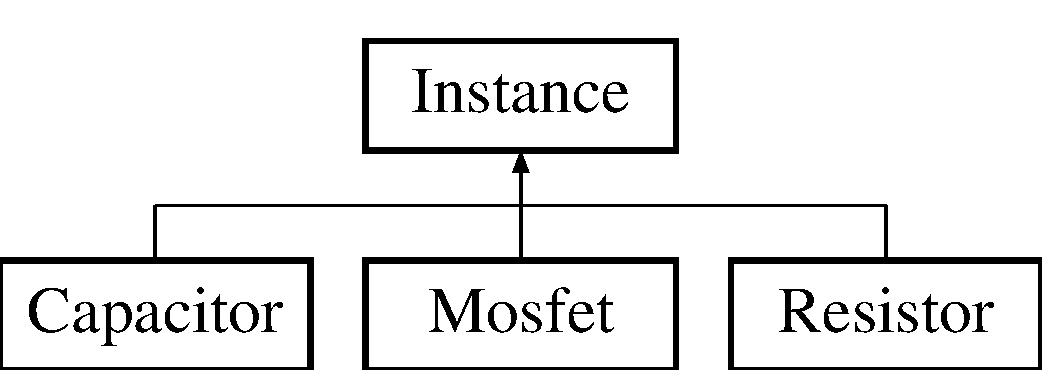
\includegraphics[height=2.000000cm]{class_s_p_i_c_e_1_1_instance}
\end{center}
\end{figure}
\subsection*{Public Member Functions}
\begin{DoxyCompactItemize}
\item 
void \hyperlink{class_s_p_i_c_e_1_1_instance_af9aeca34e780851a2b024df7c5ff5b54}{add\-Connector} (std\-::string connector)
\begin{DoxyCompactList}\small\item\em adds a connector to the instance. \end{DoxyCompactList}\item 
void \hyperlink{class_s_p_i_c_e_1_1_instance_a8d69bbbea5ece0949e100c464e412f20}{add\-Parameter} (std\-::string name, std\-::string value)
\begin{DoxyCompactList}\small\item\em add a parameter to the instance. \end{DoxyCompactList}\item 
\hypertarget{class_s_p_i_c_e_1_1_instance_acce8940edeaa3d79c522006f987e0711}{const std\-::vector$<$ std\-::string $>$ \& \hyperlink{class_s_p_i_c_e_1_1_instance_acce8940edeaa3d79c522006f987e0711}{get\-Connectors} ()}\label{class_s_p_i_c_e_1_1_instance_acce8940edeaa3d79c522006f987e0711}

\begin{DoxyCompactList}\small\item\em returns the connectors of the instance. \end{DoxyCompactList}\item 
\hypertarget{class_s_p_i_c_e_1_1_instance_afc74cbe93df9c473a53db83a325f8f9d}{std\-::string \hyperlink{class_s_p_i_c_e_1_1_instance_afc74cbe93df9c473a53db83a325f8f9d}{get\-Model} ()}\label{class_s_p_i_c_e_1_1_instance_afc74cbe93df9c473a53db83a325f8f9d}

\begin{DoxyCompactList}\small\item\em returns the model of the instance. \end{DoxyCompactList}\item 
\hypertarget{class_s_p_i_c_e_1_1_instance_ac0fc966d4386ddb71d99361e3fccb311}{std\-::string \hyperlink{class_s_p_i_c_e_1_1_instance_ac0fc966d4386ddb71d99361e3fccb311}{get\-Name} ()}\label{class_s_p_i_c_e_1_1_instance_ac0fc966d4386ddb71d99361e3fccb311}

\begin{DoxyCompactList}\small\item\em returns the name of the instance. \end{DoxyCompactList}\item 
\hypertarget{class_s_p_i_c_e_1_1_instance_aee7d59083b78d31ac5c19ab508da91e0}{const std\-::map$<$ std\-::string, \\*
std\-::string $>$ \& \hyperlink{class_s_p_i_c_e_1_1_instance_aee7d59083b78d31ac5c19ab508da91e0}{get\-Parameters} ()}\label{class_s_p_i_c_e_1_1_instance_aee7d59083b78d31ac5c19ab508da91e0}

\begin{DoxyCompactList}\small\item\em returns the parameters of the instance. \end{DoxyCompactList}\item 
std\-::string \hyperlink{class_s_p_i_c_e_1_1_instance_a324e4ff99afdcd5972d8c57461d12ef5}{get\-Parameter\-Value} (std\-::string name)
\begin{DoxyCompactList}\small\item\em returns the value (as string) of a parameter of the instance. \end{DoxyCompactList}\item 
\hyperlink{class_s_p_i_c_e_1_1_instance_a400232cdfbe82c01dd2830368377492b}{Instance} (std\-::string name, std\-::string model)
\begin{DoxyCompactList}\small\item\em creates a new instance. \end{DoxyCompactList}\end{DoxyCompactItemize}


\subsection{Detailed Description}
This class describes an instance of the global circuit. It is the base class of \hyperlink{class_s_p_i_c_e_1_1_capacitor}{S\-P\-I\-C\-E\-::\-Capacitor}, \hyperlink{class_s_p_i_c_e_1_1_mosfet}{S\-P\-I\-C\-E\-::\-Mosfet} and \hyperlink{class_s_p_i_c_e_1_1_resistor}{S\-P\-I\-C\-E\-::\-Resistor}. 

\subsection{Constructor \& Destructor Documentation}
\hypertarget{class_s_p_i_c_e_1_1_instance_a400232cdfbe82c01dd2830368377492b}{\index{S\-P\-I\-C\-E\-::\-Instance@{S\-P\-I\-C\-E\-::\-Instance}!Instance@{Instance}}
\index{Instance@{Instance}!SPICE::Instance@{S\-P\-I\-C\-E\-::\-Instance}}
\subsubsection[{Instance}]{\setlength{\rightskip}{0pt plus 5cm}{\bf Instance} (
\begin{DoxyParamCaption}
\item[{std\-::string}]{name, }
\item[{std\-::string}]{model}
\end{DoxyParamCaption}
)}}\label{class_s_p_i_c_e_1_1_instance_a400232cdfbe82c01dd2830368377492b}


creates a new instance. 


\begin{DoxyParams}{Parameters}
{\em name} & the name of the instance. \\
\hline
{\em model} & the model of the instance. \\
\hline
\end{DoxyParams}


\subsection{Member Function Documentation}
\hypertarget{class_s_p_i_c_e_1_1_instance_af9aeca34e780851a2b024df7c5ff5b54}{\index{S\-P\-I\-C\-E\-::\-Instance@{S\-P\-I\-C\-E\-::\-Instance}!add\-Connector@{add\-Connector}}
\index{add\-Connector@{add\-Connector}!SPICE::Instance@{S\-P\-I\-C\-E\-::\-Instance}}
\subsubsection[{add\-Connector}]{\setlength{\rightskip}{0pt plus 5cm}void add\-Connector (
\begin{DoxyParamCaption}
\item[{std\-::string}]{connector}
\end{DoxyParamCaption}
)\hspace{0.3cm}{\ttfamily [inline]}}}\label{class_s_p_i_c_e_1_1_instance_af9aeca34e780851a2b024df7c5ff5b54}


adds a connector to the instance. 


\begin{DoxyParams}{Parameters}
{\em connector} & the connector to add. \\
\hline
\end{DoxyParams}
\hypertarget{class_s_p_i_c_e_1_1_instance_a8d69bbbea5ece0949e100c464e412f20}{\index{S\-P\-I\-C\-E\-::\-Instance@{S\-P\-I\-C\-E\-::\-Instance}!add\-Parameter@{add\-Parameter}}
\index{add\-Parameter@{add\-Parameter}!SPICE::Instance@{S\-P\-I\-C\-E\-::\-Instance}}
\subsubsection[{add\-Parameter}]{\setlength{\rightskip}{0pt plus 5cm}void add\-Parameter (
\begin{DoxyParamCaption}
\item[{std\-::string}]{name, }
\item[{std\-::string}]{value}
\end{DoxyParamCaption}
)}}\label{class_s_p_i_c_e_1_1_instance_a8d69bbbea5ece0949e100c464e412f20}


add a parameter to the instance. 


\begin{DoxyParams}{Parameters}
{\em name} & the name of the parameter. \\
\hline
{\em value} & the value of the parameter. \\
\hline
\end{DoxyParams}
\hypertarget{class_s_p_i_c_e_1_1_instance_a324e4ff99afdcd5972d8c57461d12ef5}{\index{S\-P\-I\-C\-E\-::\-Instance@{S\-P\-I\-C\-E\-::\-Instance}!get\-Parameter\-Value@{get\-Parameter\-Value}}
\index{get\-Parameter\-Value@{get\-Parameter\-Value}!SPICE::Instance@{S\-P\-I\-C\-E\-::\-Instance}}
\subsubsection[{get\-Parameter\-Value}]{\setlength{\rightskip}{0pt plus 5cm}string get\-Parameter\-Value (
\begin{DoxyParamCaption}
\item[{std\-::string}]{name}
\end{DoxyParamCaption}
)}}\label{class_s_p_i_c_e_1_1_instance_a324e4ff99afdcd5972d8c57461d12ef5}


returns the value (as string) of a parameter of the instance. 


\begin{DoxyParams}{Parameters}
{\em name} & the name of the parameter from which to get value. \\
\hline
\end{DoxyParams}

\hypertarget{class_open_chams_1_1_instance_point}{\section{Instance\-Point Class Reference}
\label{class_open_chams_1_1_instance_point}\index{Instance\-Point@{Instance\-Point}}
}
Inheritance diagram for Instance\-Point\-:\begin{figure}[H]
\begin{center}
\leavevmode
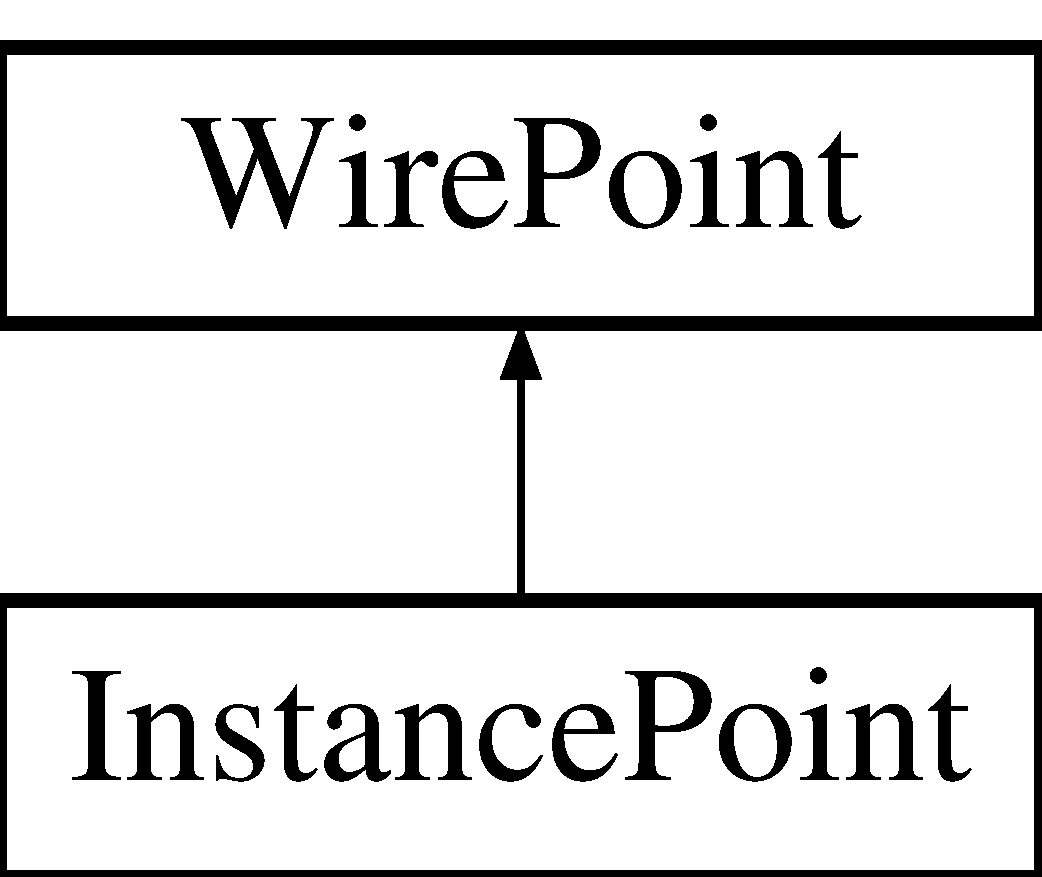
\includegraphics[height=2.000000cm]{class_open_chams_1_1_instance_point}
\end{center}
\end{figure}
\subsection*{Public Member Functions}
\begin{DoxyCompactItemize}
\item 
\hypertarget{class_open_chams_1_1_instance_point_a2858c0c4e8b5108f041237cf5a802029}{const std\-::string \& \hyperlink{class_open_chams_1_1_instance_point_a2858c0c4e8b5108f041237cf5a802029}{get\-Name} ()}\label{class_open_chams_1_1_instance_point_a2858c0c4e8b5108f041237cf5a802029}

\begin{DoxyCompactList}\small\item\em returns the name of the instance associated to the instance\-Point. \end{DoxyCompactList}\item 
\hypertarget{class_open_chams_1_1_instance_point_a646d464666fc56ab2e04a6b87fdd3279}{const std\-::string \& \hyperlink{class_open_chams_1_1_instance_point_a646d464666fc56ab2e04a6b87fdd3279}{get\-Plug} ()}\label{class_open_chams_1_1_instance_point_a646d464666fc56ab2e04a6b87fdd3279}

\begin{DoxyCompactList}\small\item\em returns the name of the connector associated to the instance\-Point. \end{DoxyCompactList}\item 
\hyperlink{class_open_chams_1_1_instance_point_a1f3b6eda5ef7bb872c96f006021a61f1}{Instance\-Point} (const std\-::string \&name, const std\-::string \&plug)
\begin{DoxyCompactList}\small\item\em creates a new wire point associated to an instance's connector. \end{DoxyCompactList}\end{DoxyCompactItemize}


\subsection{Detailed Description}
This class describes a wire point associated to an instance's connector. 

\subsection{Constructor \& Destructor Documentation}
\hypertarget{class_open_chams_1_1_instance_point_a1f3b6eda5ef7bb872c96f006021a61f1}{\index{Open\-Chams\-::\-Instance\-Point@{Open\-Chams\-::\-Instance\-Point}!Instance\-Point@{Instance\-Point}}
\index{Instance\-Point@{Instance\-Point}!OpenChams::InstancePoint@{Open\-Chams\-::\-Instance\-Point}}
\subsubsection[{Instance\-Point}]{\setlength{\rightskip}{0pt plus 5cm}{\bf Instance\-Point} (
\begin{DoxyParamCaption}
\item[{const std\-::string \&}]{name, }
\item[{const std\-::string \&}]{plug}
\end{DoxyParamCaption}
)\hspace{0.3cm}{\ttfamily [inline]}}}\label{class_open_chams_1_1_instance_point_a1f3b6eda5ef7bb872c96f006021a61f1}


creates a new wire point associated to an instance's connector. 


\begin{DoxyParams}{Parameters}
{\em name} & the name of the instance. \\
\hline
{\em connector} & the name of the connector. \\
\hline
\end{DoxyParams}

\hypertarget{class_open_chams_1_1_intermediate_point}{\section{Intermediate\-Point Class Reference}
\label{class_open_chams_1_1_intermediate_point}\index{Intermediate\-Point@{Intermediate\-Point}}
}
Inheritance diagram for Intermediate\-Point\-:\begin{figure}[H]
\begin{center}
\leavevmode
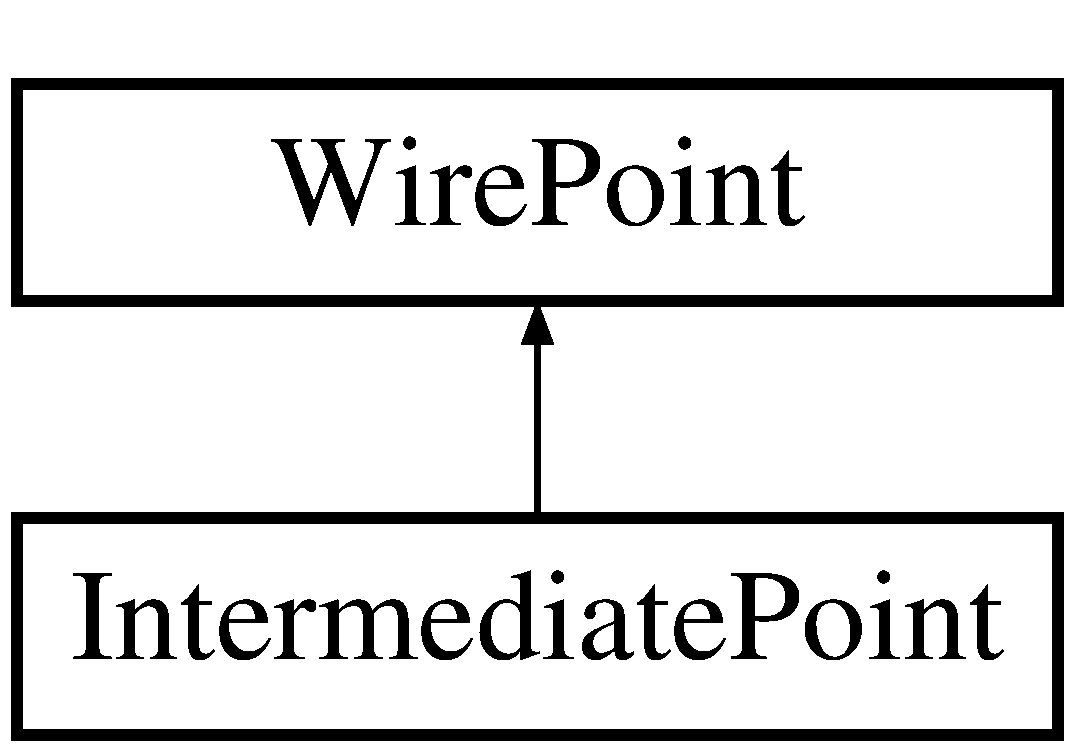
\includegraphics[height=2.000000cm]{class_open_chams_1_1_intermediate_point}
\end{center}
\end{figure}
\subsection*{Public Member Functions}
\begin{DoxyCompactItemize}
\item 
\hypertarget{class_open_chams_1_1_intermediate_point_a2b69e4312b7814c6efce42f851893409}{double \hyperlink{class_open_chams_1_1_intermediate_point_a2b69e4312b7814c6efce42f851893409}{get\-X} ()}\label{class_open_chams_1_1_intermediate_point_a2b69e4312b7814c6efce42f851893409}

\begin{DoxyCompactList}\small\item\em returns the x coordinate. \end{DoxyCompactList}\item 
\hypertarget{class_open_chams_1_1_intermediate_point_a15f19cf52955c8c3406831b288681358}{double \hyperlink{class_open_chams_1_1_intermediate_point_a15f19cf52955c8c3406831b288681358}{get\-Y} ()}\label{class_open_chams_1_1_intermediate_point_a15f19cf52955c8c3406831b288681358}

\begin{DoxyCompactList}\small\item\em returns the y coordinate. \end{DoxyCompactList}\item 
\hyperlink{class_open_chams_1_1_intermediate_point_ad8d801adfda3af856c5d1287c8bc0635}{Intermediate\-Point} (double x, double y)
\begin{DoxyCompactList}\small\item\em creates a new wire point based on its (x,y) coordinates. \end{DoxyCompactList}\end{DoxyCompactItemize}


\subsection{Detailed Description}
This class describes a wire point defined by its (x,y) coordinates. 

\subsection{Constructor \& Destructor Documentation}
\hypertarget{class_open_chams_1_1_intermediate_point_ad8d801adfda3af856c5d1287c8bc0635}{\index{Open\-Chams\-::\-Intermediate\-Point@{Open\-Chams\-::\-Intermediate\-Point}!Intermediate\-Point@{Intermediate\-Point}}
\index{Intermediate\-Point@{Intermediate\-Point}!OpenChams::IntermediatePoint@{Open\-Chams\-::\-Intermediate\-Point}}
\subsubsection[{Intermediate\-Point}]{\setlength{\rightskip}{0pt plus 5cm}{\bf Intermediate\-Point} (
\begin{DoxyParamCaption}
\item[{double}]{x, }
\item[{double}]{y}
\end{DoxyParamCaption}
)\hspace{0.3cm}{\ttfamily [inline]}}}\label{class_open_chams_1_1_intermediate_point_ad8d801adfda3af856c5d1287c8bc0635}


creates a new wire point based on its (x,y) coordinates. 


\begin{DoxyParams}{Parameters}
{\em x} & the x coordinate. \\
\hline
{\em y} & the y coordinate. \\
\hline
\end{DoxyParams}

\hypertarget{class_open_chams_1_1_layout}{}\section{Layout Class Reference}
\label{class_open_chams_1_1_layout}\index{Layout@{Layout}}
\subsection*{Public Member Functions}
\begin{DoxyCompactItemize}
\item 
void \mbox{\hyperlink{class_open_chams_1_1_layout_a4cc1899e9b782de44700fa0e4ac477ef}{add\+Instance}} (const std\+::string \&name, const std\+::string \&style)
\begin{DoxyCompactList}\small\item\em adds layout informations for a instance. \end{DoxyCompactList}\item 
\mbox{\Hypertarget{class_open_chams_1_1_layout_a13df4992219ef28a7dc014e9f5f0566a}\label{class_open_chams_1_1_layout_a13df4992219ef28a7dc014e9f5f0566a}} 
\mbox{\hyperlink{class_open_chams_1_1_node}{Node}} $\ast$ \mbox{\hyperlink{class_open_chams_1_1_layout_a13df4992219ef28a7dc014e9f5f0566a}{get\+H\+B\+Tree\+Root}} ()
\begin{DoxyCompactList}\small\item\em returns the root of the placement tree associated to the layout. \end{DoxyCompactList}\item 
\mbox{\Hypertarget{class_open_chams_1_1_layout_ab0550a9050b7e788b2a18452c9df21f7}\label{class_open_chams_1_1_layout_ab0550a9050b7e788b2a18452c9df21f7}} 
const std\+::map$<$ std\+::string, std\+::string $>$ \& \mbox{\hyperlink{class_open_chams_1_1_layout_ab0550a9050b7e788b2a18452c9df21f7}{get\+Instances}} ()
\begin{DoxyCompactList}\small\item\em returns the map of Instances. \end{DoxyCompactList}\item 
\mbox{\Hypertarget{class_open_chams_1_1_layout_af27a31f10fcf22daa64f35c9c6bd2cda}\label{class_open_chams_1_1_layout_af27a31f10fcf22daa64f35c9c6bd2cda}} 
bool \mbox{\hyperlink{class_open_chams_1_1_layout_af27a31f10fcf22daa64f35c9c6bd2cda}{has\+No\+Instance}} ()
\begin{DoxyCompactList}\small\item\em returns true if the layout has no \mbox{\hyperlink{class_open_chams_1_1_instance}{Instance}}. \end{DoxyCompactList}\item 
\mbox{\hyperlink{class_open_chams_1_1_layout_a789d82a4c563002befc83d538431d474}{Layout}} (\mbox{\hyperlink{class_open_chams_1_1_circuit}{Circuit}} $\ast$)
\begin{DoxyCompactList}\small\item\em creates a new layout. \end{DoxyCompactList}\item 
void \mbox{\hyperlink{class_open_chams_1_1_layout_a6d828958e0faf1346b27276eab101858}{set\+H\+B\+Tree\+Root}} (\mbox{\hyperlink{class_open_chams_1_1_node}{Node}} $\ast$)
\begin{DoxyCompactList}\small\item\em sets the root of the placement tree associated to the layout. \end{DoxyCompactList}\end{DoxyCompactItemize}


\subsection{Detailed Description}
This class describes layout informations for an \mbox{\hyperlink{class_open_chams_1_1_instance}{Instance}}.

The \mbox{\hyperlink{class_open_chams_1_1_layout}{Layout}} object is used to store all informations relative to physical layout of the instance (such as the layout style).

\begin{DoxyNote}{Note}
The \mbox{\hyperlink{class_open_chams_1_1_layout}{Layout}} object is optionnal in \mbox{\hyperlink{class_open_chams_1_1_circuit}{Circuit}}. 
\end{DoxyNote}


\subsection{Constructor \& Destructor Documentation}
\mbox{\Hypertarget{class_open_chams_1_1_layout_a789d82a4c563002befc83d538431d474}\label{class_open_chams_1_1_layout_a789d82a4c563002befc83d538431d474}} 
\index{Open\+Chams\+::\+Layout@{Open\+Chams\+::\+Layout}!Layout@{Layout}}
\index{Layout@{Layout}!Open\+Chams\+::\+Layout@{Open\+Chams\+::\+Layout}}
\subsubsection{\texorpdfstring{Layout()}{Layout()}}
{\footnotesize\ttfamily \mbox{\hyperlink{class_open_chams_1_1_layout}{Layout}} (\begin{DoxyParamCaption}\item[{\mbox{\hyperlink{class_open_chams_1_1_circuit}{Circuit}} $\ast$}]{circuit }\end{DoxyParamCaption})}



creates a new layout. 


\begin{DoxyParams}{Parameters}
{\em circuit} & the circuit to which the layout belongs. \\
\hline
\end{DoxyParams}


\subsection{Member Function Documentation}
\mbox{\Hypertarget{class_open_chams_1_1_layout_a4cc1899e9b782de44700fa0e4ac477ef}\label{class_open_chams_1_1_layout_a4cc1899e9b782de44700fa0e4ac477ef}} 
\index{Open\+Chams\+::\+Layout@{Open\+Chams\+::\+Layout}!add\+Instance@{add\+Instance}}
\index{add\+Instance@{add\+Instance}!Open\+Chams\+::\+Layout@{Open\+Chams\+::\+Layout}}
\subsubsection{\texorpdfstring{add\+Instance()}{addInstance()}}
{\footnotesize\ttfamily void add\+Instance (\begin{DoxyParamCaption}\item[{const std\+::string \&}]{name,  }\item[{const std\+::string \&}]{style }\end{DoxyParamCaption})}



adds layout informations for a instance. 


\begin{DoxyParams}{Parameters}
{\em name} & the instance\textquotesingle{}s name to which the layout is associated. \\
\hline
{\em style} & the layout style. \\
\hline
\end{DoxyParams}
\mbox{\Hypertarget{class_open_chams_1_1_layout_a6d828958e0faf1346b27276eab101858}\label{class_open_chams_1_1_layout_a6d828958e0faf1346b27276eab101858}} 
\index{Open\+Chams\+::\+Layout@{Open\+Chams\+::\+Layout}!set\+H\+B\+Tree\+Root@{set\+H\+B\+Tree\+Root}}
\index{set\+H\+B\+Tree\+Root@{set\+H\+B\+Tree\+Root}!Open\+Chams\+::\+Layout@{Open\+Chams\+::\+Layout}}
\subsubsection{\texorpdfstring{set\+H\+B\+Tree\+Root()}{setHBTreeRoot()}}
{\footnotesize\ttfamily void set\+H\+B\+Tree\+Root (\begin{DoxyParamCaption}\item[{\mbox{\hyperlink{class_open_chams_1_1_node}{Node}} $\ast$}]{root }\end{DoxyParamCaption})\hspace{0.3cm}{\ttfamily [inline]}}



sets the root of the placement tree associated to the layout. 


\begin{DoxyParams}{Parameters}
{\em root} & the root of the palcement tree. \\
\hline
\end{DoxyParams}

\hypertarget{class_a_g_d_s_1_1_library}{}\section{Library Class Reference}
\label{class_a_g_d_s_1_1_library}\index{Library@{Library}}
\subsection*{Public Member Functions}
\begin{DoxyCompactItemize}
\item 
bool \mbox{\hyperlink{class_a_g_d_s_1_1_library_a93d333a20154e0b688ff3ff213039171}{add\+Structure}} (\mbox{\hyperlink{class_a_g_d_s_1_1_structure}{Structure}} $\ast$)
\begin{DoxyCompactList}\small\item\em adds a \mbox{\hyperlink{class_a_g_d_s_1_1_structure}{Structure}} to the \mbox{\hyperlink{class_a_g_d_s_1_1_library}{Library}}. \end{DoxyCompactList}\item 
\mbox{\hyperlink{class_a_g_d_s_1_1_library_a9244ebe2cc60781aaf25cf559ea2473a}{Library}} (std\+::string lib\+Name)
\begin{DoxyCompactList}\small\item\em creates a new \mbox{\hyperlink{class_a_g_d_s_1_1_library}{Library}} \end{DoxyCompactList}\item 
void \mbox{\hyperlink{class_a_g_d_s_1_1_library_a938acb6eb8d14aade9dba7331c75ff0a}{set\+Phys\+Units}} (double phys\+Units)
\begin{DoxyCompactList}\small\item\em sets the physical units. \end{DoxyCompactList}\item 
void \mbox{\hyperlink{class_a_g_d_s_1_1_library_a0d0e972bb142f892c462bb8d7f04a50b}{set\+User\+Units}} (double user\+Units)
\begin{DoxyCompactList}\small\item\em sets the user units. \end{DoxyCompactList}\item 
bool \mbox{\hyperlink{class_a_g_d_s_1_1_library_a33b9d989b84857f46034085664ff3fa2}{write\+To\+File}} (std\+::string file\+Name)
\begin{DoxyCompactList}\small\item\em writes the database to file. \end{DoxyCompactList}\end{DoxyCompactItemize}


\subsection{Detailed Description}
This class contains all A\+G\+DS library informations such as the name, the unit used (user and physical) and the list of all Structures. 

\subsection{Constructor \& Destructor Documentation}
\mbox{\Hypertarget{class_a_g_d_s_1_1_library_a9244ebe2cc60781aaf25cf559ea2473a}\label{class_a_g_d_s_1_1_library_a9244ebe2cc60781aaf25cf559ea2473a}} 
\index{A\+G\+D\+S\+::\+Library@{A\+G\+D\+S\+::\+Library}!Library@{Library}}
\index{Library@{Library}!A\+G\+D\+S\+::\+Library@{A\+G\+D\+S\+::\+Library}}
\subsubsection{\texorpdfstring{Library()}{Library()}}
{\footnotesize\ttfamily \mbox{\hyperlink{class_a_g_d_s_1_1_library}{Library}} (\begin{DoxyParamCaption}\item[{std\+::string}]{name }\end{DoxyParamCaption})}



creates a new \mbox{\hyperlink{class_a_g_d_s_1_1_library}{Library}} 


\begin{DoxyParams}{Parameters}
{\em name} & the name of the library. \\
\hline
\end{DoxyParams}


\subsection{Member Function Documentation}
\mbox{\Hypertarget{class_a_g_d_s_1_1_library_a93d333a20154e0b688ff3ff213039171}\label{class_a_g_d_s_1_1_library_a93d333a20154e0b688ff3ff213039171}} 
\index{A\+G\+D\+S\+::\+Library@{A\+G\+D\+S\+::\+Library}!add\+Structure@{add\+Structure}}
\index{add\+Structure@{add\+Structure}!A\+G\+D\+S\+::\+Library@{A\+G\+D\+S\+::\+Library}}
\subsubsection{\texorpdfstring{add\+Structure()}{addStructure()}}
{\footnotesize\ttfamily bool add\+Structure (\begin{DoxyParamCaption}\item[{\mbox{\hyperlink{class_a_g_d_s_1_1_structure}{Structure}} $\ast$}]{str }\end{DoxyParamCaption})}



adds a \mbox{\hyperlink{class_a_g_d_s_1_1_structure}{Structure}} to the \mbox{\hyperlink{class_a_g_d_s_1_1_library}{Library}}. 


\begin{DoxyParams}{Parameters}
{\em str} & the \mbox{\hyperlink{class_a_g_d_s_1_1_structure}{Structure}} object to add. \\
\hline
\end{DoxyParams}
\mbox{\Hypertarget{class_a_g_d_s_1_1_library_a938acb6eb8d14aade9dba7331c75ff0a}\label{class_a_g_d_s_1_1_library_a938acb6eb8d14aade9dba7331c75ff0a}} 
\index{A\+G\+D\+S\+::\+Library@{A\+G\+D\+S\+::\+Library}!set\+Phys\+Units@{set\+Phys\+Units}}
\index{set\+Phys\+Units@{set\+Phys\+Units}!A\+G\+D\+S\+::\+Library@{A\+G\+D\+S\+::\+Library}}
\subsubsection{\texorpdfstring{set\+Phys\+Units()}{setPhysUnits()}}
{\footnotesize\ttfamily void set\+Phys\+Units (\begin{DoxyParamCaption}\item[{double}]{phys\+Units }\end{DoxyParamCaption})\hspace{0.3cm}{\ttfamily [inline]}}



sets the physical units. 


\begin{DoxyParams}{Parameters}
{\em phys\+Units} & the value of the physical units. \\
\hline
\end{DoxyParams}
\mbox{\Hypertarget{class_a_g_d_s_1_1_library_a0d0e972bb142f892c462bb8d7f04a50b}\label{class_a_g_d_s_1_1_library_a0d0e972bb142f892c462bb8d7f04a50b}} 
\index{A\+G\+D\+S\+::\+Library@{A\+G\+D\+S\+::\+Library}!set\+User\+Units@{set\+User\+Units}}
\index{set\+User\+Units@{set\+User\+Units}!A\+G\+D\+S\+::\+Library@{A\+G\+D\+S\+::\+Library}}
\subsubsection{\texorpdfstring{set\+User\+Units()}{setUserUnits()}}
{\footnotesize\ttfamily void set\+User\+Units (\begin{DoxyParamCaption}\item[{double}]{user\+Units }\end{DoxyParamCaption})\hspace{0.3cm}{\ttfamily [inline]}}



sets the user units. 


\begin{DoxyParams}{Parameters}
{\em user\+Units} & the value of the user units. \\
\hline
\end{DoxyParams}
\mbox{\Hypertarget{class_a_g_d_s_1_1_library_a33b9d989b84857f46034085664ff3fa2}\label{class_a_g_d_s_1_1_library_a33b9d989b84857f46034085664ff3fa2}} 
\index{A\+G\+D\+S\+::\+Library@{A\+G\+D\+S\+::\+Library}!write\+To\+File@{write\+To\+File}}
\index{write\+To\+File@{write\+To\+File}!A\+G\+D\+S\+::\+Library@{A\+G\+D\+S\+::\+Library}}
\subsubsection{\texorpdfstring{write\+To\+File()}{writeToFile()}}
{\footnotesize\ttfamily bool write\+To\+File (\begin{DoxyParamCaption}\item[{std\+::string}]{filename }\end{DoxyParamCaption})}



writes the database to file. 


\begin{DoxyParams}{Parameters}
{\em filename} & the destination file name.\\
\hline
\end{DoxyParams}
\begin{DoxyNote}{Note}
When driving file, current date and time are used to define date in generated C\+IF file. 
\end{DoxyNote}

\hypertarget{struct_open_chams_1_1map__item}{\section{map\-\_\-item$<$ Key, Val $>$ Struct Template Reference}
\label{struct_open_chams_1_1map__item}\index{map\-\_\-item$<$ Key, Val $>$@{map\-\_\-item$<$ Key, Val $>$}}
}

\hypertarget{struct_s_p_i_c_e_1_1map__item}{\section{map\-\_\-item$<$ Key, Val $>$ Struct Template Reference}
\label{struct_s_p_i_c_e_1_1map__item}\index{map\-\_\-item$<$ Key, Val $>$@{map\-\_\-item$<$ Key, Val $>$}}
}

\hypertarget{class_s_p_i_c_e_1_1_mosfet}{}\section{Mosfet Class Reference}
\label{class_s_p_i_c_e_1_1_mosfet}\index{Mosfet@{Mosfet}}
Inheritance diagram for Mosfet\+:\begin{figure}[H]
\begin{center}
\leavevmode
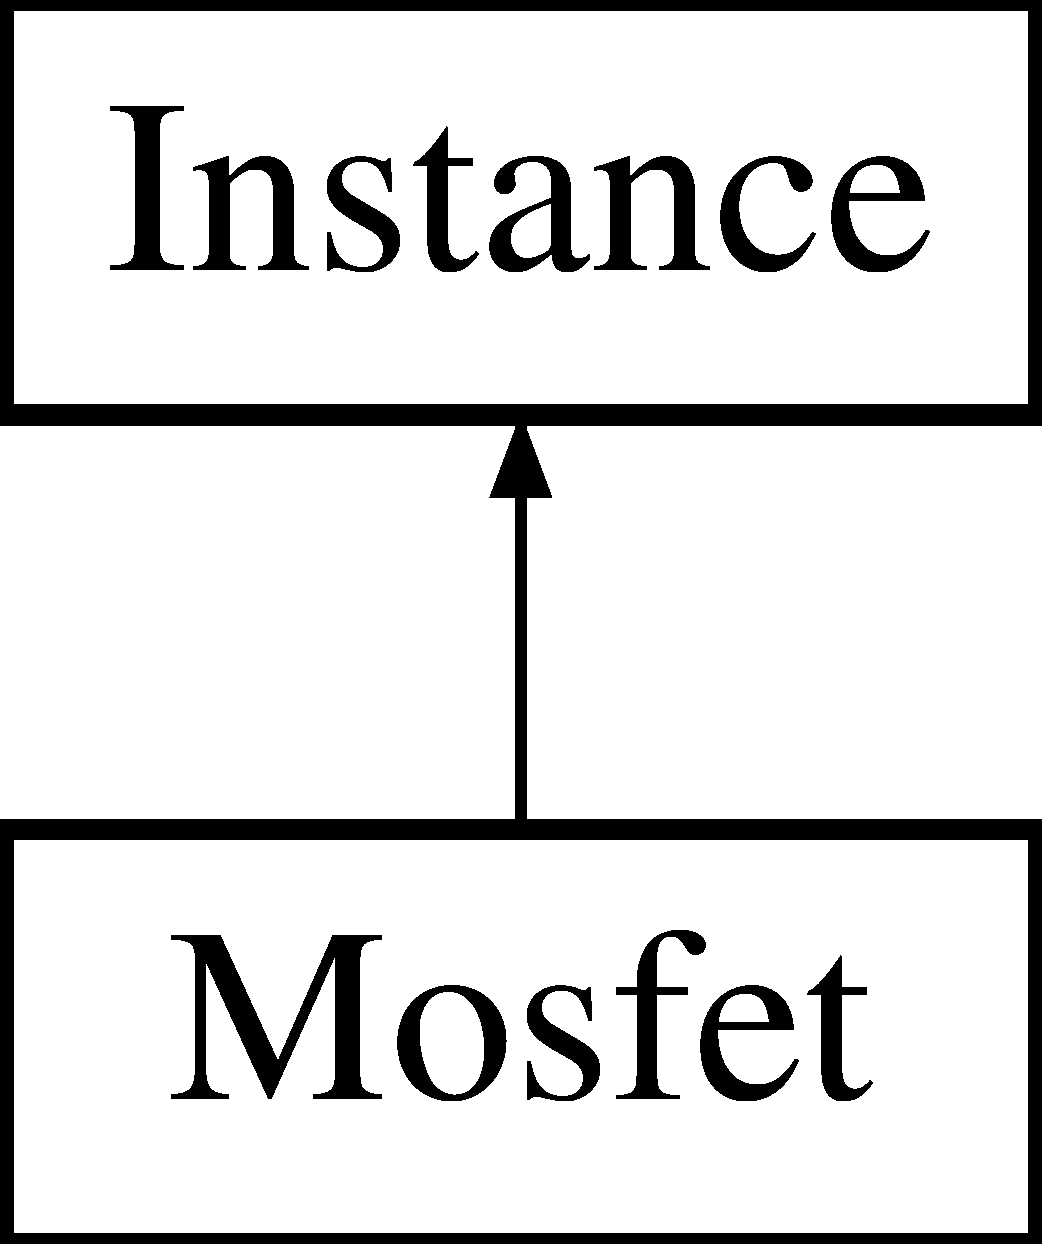
\includegraphics[height=2.000000cm]{class_s_p_i_c_e_1_1_mosfet}
\end{center}
\end{figure}
\subsection*{Public Member Functions}
\begin{DoxyCompactItemize}
\item 
\mbox{\Hypertarget{class_s_p_i_c_e_1_1_mosfet_a56484a169335450d6043ee20086ead93}\label{class_s_p_i_c_e_1_1_mosfet_a56484a169335450d6043ee20086ead93}} 
std\+::string \hyperlink{class_s_p_i_c_e_1_1_mosfet_a56484a169335450d6043ee20086ead93}{get\+Bulk} ()
\begin{DoxyCompactList}\small\item\em returns the bulk connector of the transistor. \end{DoxyCompactList}\item 
\mbox{\Hypertarget{class_s_p_i_c_e_1_1_mosfet_a7265f0565b8368070a3f09c6197a4e9b}\label{class_s_p_i_c_e_1_1_mosfet_a7265f0565b8368070a3f09c6197a4e9b}} 
std\+::string \hyperlink{class_s_p_i_c_e_1_1_mosfet_a7265f0565b8368070a3f09c6197a4e9b}{get\+Drain} ()
\begin{DoxyCompactList}\small\item\em returns the drain connector of the transistor. \end{DoxyCompactList}\item 
\mbox{\Hypertarget{class_s_p_i_c_e_1_1_mosfet_a796d77755aac0828419f55ba2226bf15}\label{class_s_p_i_c_e_1_1_mosfet_a796d77755aac0828419f55ba2226bf15}} 
std\+::string \hyperlink{class_s_p_i_c_e_1_1_mosfet_a796d77755aac0828419f55ba2226bf15}{get\+Grid} ()
\begin{DoxyCompactList}\small\item\em returns the grid connector of the transistor. \end{DoxyCompactList}\item 
\mbox{\Hypertarget{class_s_p_i_c_e_1_1_mosfet_a1791f52b6b5043823c6f3376e8453e3a}\label{class_s_p_i_c_e_1_1_mosfet_a1791f52b6b5043823c6f3376e8453e3a}} 
std\+::string \hyperlink{class_s_p_i_c_e_1_1_mosfet_a1791f52b6b5043823c6f3376e8453e3a}{get\+Source} ()
\begin{DoxyCompactList}\small\item\em returns the source connector of the transistor. \end{DoxyCompactList}\item 
\hyperlink{class_s_p_i_c_e_1_1_mosfet_a4f54a31aad6137a6426fb9bfe8947bcf}{Mosfet} (std\+::string name, std\+::string nd, std\+::string ng, std\+::string ns, std\+::string nb, std\+::string model)
\begin{DoxyCompactList}\small\item\em creates a new mosfet transistor. \end{DoxyCompactList}\end{DoxyCompactItemize}


\subsection{Detailed Description}
This class describes a mosfet transistor which is a specialized instance which has four connectors (grid, drain, source and bulk). 

\subsection{Constructor \& Destructor Documentation}
\mbox{\Hypertarget{class_s_p_i_c_e_1_1_mosfet_a4f54a31aad6137a6426fb9bfe8947bcf}\label{class_s_p_i_c_e_1_1_mosfet_a4f54a31aad6137a6426fb9bfe8947bcf}} 
\index{S\+P\+I\+C\+E\+::\+Mosfet@{S\+P\+I\+C\+E\+::\+Mosfet}!Mosfet@{Mosfet}}
\index{Mosfet@{Mosfet}!S\+P\+I\+C\+E\+::\+Mosfet@{S\+P\+I\+C\+E\+::\+Mosfet}}
\subsubsection{\texorpdfstring{Mosfet()}{Mosfet()}}
{\footnotesize\ttfamily \hyperlink{class_s_p_i_c_e_1_1_mosfet}{Mosfet} (\begin{DoxyParamCaption}\item[{std\+::string}]{name,  }\item[{std\+::string}]{drain,  }\item[{std\+::string}]{grid,  }\item[{std\+::string}]{source,  }\item[{std\+::string}]{bulk,  }\item[{std\+::string}]{model }\end{DoxyParamCaption})\hspace{0.3cm}{\ttfamily [inline]}}



creates a new mosfet transistor. 


\begin{DoxyParams}{Parameters}
{\em name} & the name of the transistor. \\
\hline
{\em drain} & the drain connector of the transistor. \\
\hline
{\em grid} & the grid connector of the transistor. \\
\hline
{\em source} & the source connector of the transistor. \\
\hline
{\em bulk} & the bulk connector of the transistor. \\
\hline
{\em model} & the model of the transistor. \\
\hline
\end{DoxyParams}

\hypertarget{class_name}{\section{Name Class Reference}
\label{class_name}\index{Name@{Name}}
}


\subsection{Detailed Description}
This class provides an automatic management of shared name. 
\hypertarget{class_open_chams_1_1_net}{}\section{Net Class Reference}
\label{class_open_chams_1_1_net}\index{Net@{Net}}
\subsection*{Data Structures}
\begin{DoxyCompactItemize}
\item 
class \mbox{\hyperlink{class_open_chams_1_1_net_1_1_connection}{Connection}}
\end{DoxyCompactItemize}
\subsection*{Public Member Functions}
\begin{DoxyCompactItemize}
\item 
\mbox{\hyperlink{class_open_chams_1_1_port}{Port}} $\ast$ \mbox{\hyperlink{class_open_chams_1_1_net_af395a7c9d6f3c2b24500b91260873664}{add\+Port}} (const std\+::string \&type, unsigned idx, double x, double y, const std\+::string \&orient)
\begin{DoxyCompactList}\small\item\em adds a \mbox{\hyperlink{class_open_chams_1_1_port}{Port}} to the net. \end{DoxyCompactList}\item 
\mbox{\hyperlink{class_open_chams_1_1_wire}{Wire}} $\ast$ \mbox{\hyperlink{class_open_chams_1_1_net_a643a969f62770301b8b70ed63c36a55e}{add\+Wire}} ()
\begin{DoxyCompactList}\small\item\em adds a \mbox{\hyperlink{class_open_chams_1_1_wire}{Wire}} to the net. \end{DoxyCompactList}\item 
void \mbox{\hyperlink{class_open_chams_1_1_net_a40c2c019175ba3bfa4b90f4ad5d06483}{connect\+To}} (const std\+::string \&instance\+Name, const std\+::string \&connector\+Name)
\begin{DoxyCompactList}\small\item\em adds a connection to the net. \end{DoxyCompactList}\item 
\mbox{\Hypertarget{class_open_chams_1_1_net_a87e7c71b25171dd479af0488865c8179}\label{class_open_chams_1_1_net_a87e7c71b25171dd479af0488865c8179}} 
const std\+::vector$<$ \mbox{\hyperlink{class_open_chams_1_1_net_1_1_connection}{Net\+::\+Connection}} $\ast$ $>$ \& \mbox{\hyperlink{class_open_chams_1_1_net_a87e7c71b25171dd479af0488865c8179}{get\+Connections}} ()
\begin{DoxyCompactList}\small\item\em returns the list of net\textquotesingle{}s connections. \end{DoxyCompactList}\item 
\mbox{\Hypertarget{class_open_chams_1_1_net_a3fd7335faa33dce2f87c7e50eef3e294}\label{class_open_chams_1_1_net_a3fd7335faa33dce2f87c7e50eef3e294}} 
const std\+::string \& \mbox{\hyperlink{class_open_chams_1_1_net_a3fd7335faa33dce2f87c7e50eef3e294}{get\+Name}} () const
\begin{DoxyCompactList}\small\item\em returns the name of the net. \end{DoxyCompactList}\item 
\mbox{\Hypertarget{class_open_chams_1_1_net_a4085d6a7b6958ffdd7ab5df7e6d6e53f}\label{class_open_chams_1_1_net_a4085d6a7b6958ffdd7ab5df7e6d6e53f}} 
\mbox{\hyperlink{class_open_chams_1_1_netlist}{Netlist}} $\ast$ \mbox{\hyperlink{class_open_chams_1_1_net_a4085d6a7b6958ffdd7ab5df7e6d6e53f}{get\+Netlist}} ()
\begin{DoxyCompactList}\small\item\em returns the \mbox{\hyperlink{class_open_chams_1_1_netlist}{Netlist}} to which the net belongs. \end{DoxyCompactList}\item 
\mbox{\Hypertarget{class_open_chams_1_1_net_ae9d241ec6dd833b6d7813e14ff2d9eca}\label{class_open_chams_1_1_net_ae9d241ec6dd833b6d7813e14ff2d9eca}} 
const std\+::vector$<$ \mbox{\hyperlink{class_open_chams_1_1_port}{Port}} $\ast$ $>$ \& \mbox{\hyperlink{class_open_chams_1_1_net_ae9d241ec6dd833b6d7813e14ff2d9eca}{get\+Ports}} ()
\begin{DoxyCompactList}\small\item\em returns the list of net\textquotesingle{}s \mbox{\hyperlink{class_open_chams_1_1_port}{Port}}. \end{DoxyCompactList}\item 
\mbox{\Hypertarget{class_open_chams_1_1_net_a7a88ff26f0ba9cfbfa5059c565d1e30b}\label{class_open_chams_1_1_net_a7a88ff26f0ba9cfbfa5059c565d1e30b}} 
const std\+::string \& \mbox{\hyperlink{class_open_chams_1_1_net_a7a88ff26f0ba9cfbfa5059c565d1e30b}{get\+Type}} ()
\begin{DoxyCompactList}\small\item\em returns the type of the net. \end{DoxyCompactList}\item 
\mbox{\Hypertarget{class_open_chams_1_1_net_a2f8bcf7cad7711850efeca408f146b8a}\label{class_open_chams_1_1_net_a2f8bcf7cad7711850efeca408f146b8a}} 
const std\+::vector$<$ \mbox{\hyperlink{class_open_chams_1_1_wire}{Wire}} $\ast$ $>$ \& \mbox{\hyperlink{class_open_chams_1_1_net_a2f8bcf7cad7711850efeca408f146b8a}{get\+Wires}} ()
\begin{DoxyCompactList}\small\item\em returns the list of net\textquotesingle{}s \mbox{\hyperlink{class_open_chams_1_1_wire}{Wire}}. \end{DoxyCompactList}\item 
\mbox{\Hypertarget{class_open_chams_1_1_net_ac4a660a2f87ab816f6e8b5ae2c2142f9}\label{class_open_chams_1_1_net_ac4a660a2f87ab816f6e8b5ae2c2142f9}} 
bool \mbox{\hyperlink{class_open_chams_1_1_net_ac4a660a2f87ab816f6e8b5ae2c2142f9}{has\+No\+Connections}} ()
\begin{DoxyCompactList}\small\item\em returns true if the net has no \mbox{\hyperlink{class_open_chams_1_1_net_1_1_connection}{Net\+::\+Connection}}. \end{DoxyCompactList}\item 
\mbox{\Hypertarget{class_open_chams_1_1_net_a3eef7a6d1e945441f197f0918ab8895e}\label{class_open_chams_1_1_net_a3eef7a6d1e945441f197f0918ab8895e}} 
bool \mbox{\hyperlink{class_open_chams_1_1_net_a3eef7a6d1e945441f197f0918ab8895e}{has\+No\+Ports}} ()
\begin{DoxyCompactList}\small\item\em returns true if net has no \mbox{\hyperlink{class_open_chams_1_1_port}{Port}}. \end{DoxyCompactList}\item 
\mbox{\Hypertarget{class_open_chams_1_1_net_ac9470e72b26d4cddef3d13e69057ee54}\label{class_open_chams_1_1_net_ac9470e72b26d4cddef3d13e69057ee54}} 
bool \mbox{\hyperlink{class_open_chams_1_1_net_ac9470e72b26d4cddef3d13e69057ee54}{has\+No\+Wires}} ()
\begin{DoxyCompactList}\small\item\em returns true if net has no \mbox{\hyperlink{class_open_chams_1_1_wire}{Wire}}. \end{DoxyCompactList}\item 
\mbox{\Hypertarget{class_open_chams_1_1_net_ab2570574db49633f58f7b64099d6852c}\label{class_open_chams_1_1_net_ab2570574db49633f58f7b64099d6852c}} 
bool \mbox{\hyperlink{class_open_chams_1_1_net_ab2570574db49633f58f7b64099d6852c}{is\+External}} ()
\begin{DoxyCompactList}\small\item\em returns true if the net is external. \end{DoxyCompactList}\item 
\mbox{\hyperlink{class_open_chams_1_1_net_a471976cf479ec4b1f521923d3a4e617d}{Net}} (const std\+::string \&net\+Name, const std\+::string \&type\+Name, bool, \mbox{\hyperlink{class_open_chams_1_1_netlist}{Netlist}} $\ast$)
\begin{DoxyCompactList}\small\item\em creates a new net. \end{DoxyCompactList}\end{DoxyCompactItemize}


\subsection{Detailed Description}
This class describes a \mbox{\hyperlink{class_open_chams_1_1_net}{Net}}. 

\subsection{Constructor \& Destructor Documentation}
\mbox{\Hypertarget{class_open_chams_1_1_net_a471976cf479ec4b1f521923d3a4e617d}\label{class_open_chams_1_1_net_a471976cf479ec4b1f521923d3a4e617d}} 
\index{Open\+Chams\+::\+Net@{Open\+Chams\+::\+Net}!Net@{Net}}
\index{Net@{Net}!Open\+Chams\+::\+Net@{Open\+Chams\+::\+Net}}
\subsubsection{\texorpdfstring{Net()}{Net()}}
{\footnotesize\ttfamily \mbox{\hyperlink{class_open_chams_1_1_net}{Net}} (\begin{DoxyParamCaption}\item[{const std\+::string \&}]{net\+Name,  }\item[{const std\+::string \&}]{type\+Name,  }\item[{bool}]{is\+External,  }\item[{\mbox{\hyperlink{class_open_chams_1_1_netlist}{Netlist}} $\ast$}]{netlist }\end{DoxyParamCaption})}



creates a new net. 


\begin{DoxyParams}{Parameters}
{\em name} & the name of the net. \\
\hline
{\em type} & the type of the net (L\+O\+G\+I\+C\+AL, P\+O\+W\+ER, G\+R\+O\+U\+ND, ...). \\
\hline
{\em external} & if true, then the net is set as external. \\
\hline
{\em netlist} & the netlist to which the transistor belongs. \\
\hline
\end{DoxyParams}


\subsection{Member Function Documentation}
\mbox{\Hypertarget{class_open_chams_1_1_net_af395a7c9d6f3c2b24500b91260873664}\label{class_open_chams_1_1_net_af395a7c9d6f3c2b24500b91260873664}} 
\index{Open\+Chams\+::\+Net@{Open\+Chams\+::\+Net}!add\+Port@{add\+Port}}
\index{add\+Port@{add\+Port}!Open\+Chams\+::\+Net@{Open\+Chams\+::\+Net}}
\subsubsection{\texorpdfstring{add\+Port()}{addPort()}}
{\footnotesize\ttfamily \mbox{\hyperlink{class_open_chams_1_1_port}{Port}} $\ast$ add\+Port (\begin{DoxyParamCaption}\item[{const std\+::string \&}]{type,  }\item[{unsigned}]{idx,  }\item[{double}]{x,  }\item[{double}]{y,  }\item[{const std\+::string \&}]{orient }\end{DoxyParamCaption})}



adds a \mbox{\hyperlink{class_open_chams_1_1_port}{Port}} to the net. 


\begin{DoxyParams}{Parameters}
{\em type} & the type of the port. \\
\hline
{\em idx} & the index of the port. \\
\hline
{\em x} & the x coordinate of the port. \\
\hline
{\em y} & the y coordinate of the port. \\
\hline
{\em orient} & the orientation of the port.\\
\hline
\end{DoxyParams}
\begin{DoxyReturn}{Returns}
the newly created \mbox{\hyperlink{class_open_chams_1_1_port}{Port}}. 
\end{DoxyReturn}
\mbox{\Hypertarget{class_open_chams_1_1_net_a643a969f62770301b8b70ed63c36a55e}\label{class_open_chams_1_1_net_a643a969f62770301b8b70ed63c36a55e}} 
\index{Open\+Chams\+::\+Net@{Open\+Chams\+::\+Net}!add\+Wire@{add\+Wire}}
\index{add\+Wire@{add\+Wire}!Open\+Chams\+::\+Net@{Open\+Chams\+::\+Net}}
\subsubsection{\texorpdfstring{add\+Wire()}{addWire()}}
{\footnotesize\ttfamily \mbox{\hyperlink{class_open_chams_1_1_wire}{Wire}} $\ast$ add\+Wire (\begin{DoxyParamCaption}{ }\end{DoxyParamCaption})}



adds a \mbox{\hyperlink{class_open_chams_1_1_wire}{Wire}} to the net. 

\begin{DoxyReturn}{Returns}
the newly create \mbox{\hyperlink{class_open_chams_1_1_wire}{Wire}}. 
\end{DoxyReturn}
\mbox{\Hypertarget{class_open_chams_1_1_net_a40c2c019175ba3bfa4b90f4ad5d06483}\label{class_open_chams_1_1_net_a40c2c019175ba3bfa4b90f4ad5d06483}} 
\index{Open\+Chams\+::\+Net@{Open\+Chams\+::\+Net}!connect\+To@{connect\+To}}
\index{connect\+To@{connect\+To}!Open\+Chams\+::\+Net@{Open\+Chams\+::\+Net}}
\subsubsection{\texorpdfstring{connect\+To()}{connectTo()}}
{\footnotesize\ttfamily void connect\+To (\begin{DoxyParamCaption}\item[{const std\+::string \&}]{instance\+Name,  }\item[{const std\+::string \&}]{connector\+Name }\end{DoxyParamCaption})}



adds a connection to the net. 


\begin{DoxyParams}{Parameters}
{\em instance\+Name} & the instance\textquotesingle{}s name of the \mbox{\hyperlink{class_open_chams_1_1_net_1_1_connection}{Net\+::\+Connection}}. \\
\hline
{\em connector\+Name} & the connector\textquotesingle{}s name ot the \mbox{\hyperlink{class_open_chams_1_1_net_1_1_connection}{Net\+::\+Connection}}. \\
\hline
\end{DoxyParams}

\hypertarget{class_open_chams_1_1_netlist}{}\section{Netlist Class Reference}
\label{class_open_chams_1_1_netlist}\index{Netlist@{Netlist}}
\subsection*{Public Member Functions}
\begin{DoxyCompactItemize}
\item 
\mbox{\hyperlink{class_open_chams_1_1_device}{Device}} $\ast$ \mbox{\hyperlink{class_open_chams_1_1_netlist_a8e1798a2516c32fbab629ce8d60d4b1d}{add\+Device}} (const std\+::string \&name, const std\+::string \&model, unsigned, const std\+::string \&mos\+Type, bool)
\begin{DoxyCompactList}\small\item\em adds a \mbox{\hyperlink{class_open_chams_1_1_device}{Device}} to the netlist. \end{DoxyCompactList}\item 
\mbox{\hyperlink{class_open_chams_1_1_instance}{Instance}} $\ast$ \mbox{\hyperlink{class_open_chams_1_1_netlist_af0fb73e5e8589a64d13b6d8104a34a03}{add\+Instance}} (const std\+::string \&name, const std\+::string \&model, unsigned)
\begin{DoxyCompactList}\small\item\em adds an \mbox{\hyperlink{class_open_chams_1_1_instance}{Instance}} (subcircuit) to the netlist. \end{DoxyCompactList}\item 
\mbox{\hyperlink{class_open_chams_1_1_net}{Net}} $\ast$ \mbox{\hyperlink{class_open_chams_1_1_netlist_a52be455a704925328843770552eca43d}{add\+Net}} (const std\+::string \&name, const std\+::string \&type, bool)
\begin{DoxyCompactList}\small\item\em adds a \mbox{\hyperlink{class_open_chams_1_1_net}{Net}} to the netlist. \end{DoxyCompactList}\item 
\mbox{\Hypertarget{class_open_chams_1_1_netlist_a01673b4356977793545c5f3a55ceaba5}\label{class_open_chams_1_1_netlist_a01673b4356977793545c5f3a55ceaba5}} 
\mbox{\hyperlink{class_open_chams_1_1_circuit}{Circuit}} $\ast$ \mbox{\hyperlink{class_open_chams_1_1_netlist_a01673b4356977793545c5f3a55ceaba5}{get\+Circuit}} ()
\begin{DoxyCompactList}\small\item\em returns the \mbox{\hyperlink{class_open_chams_1_1_circuit}{Circuit}} the netlist is associated to. \end{DoxyCompactList}\item 
\mbox{\hyperlink{class_open_chams_1_1_instance}{Instance}} $\ast$ \mbox{\hyperlink{class_open_chams_1_1_netlist_a6fbcd8c819bd0b576398ac031c2726fc}{get\+Instance}} (const std\+::string \&)
\begin{DoxyCompactList}\small\item\em returns the \mbox{\hyperlink{class_open_chams_1_1_instance}{Instance}} named {\ttfamily name} or N\+U\+LL it does not exist. \end{DoxyCompactList}\item 
\mbox{\Hypertarget{class_open_chams_1_1_netlist_a8e6e58ffab876152a740092520c35d73}\label{class_open_chams_1_1_netlist_a8e6e58ffab876152a740092520c35d73}} 
const std\+::vector$<$ \mbox{\hyperlink{class_open_chams_1_1_instance}{Instance}} $\ast$ $>$ \& \mbox{\hyperlink{class_open_chams_1_1_netlist_a8e6e58ffab876152a740092520c35d73}{get\+Instances}} ()
\begin{DoxyCompactList}\small\item\em returns the list of netlist\textquotesingle{}s instances. \end{DoxyCompactList}\item 
\mbox{\hyperlink{class_open_chams_1_1_net}{Net}} $\ast$ \mbox{\hyperlink{class_open_chams_1_1_netlist_a18b468cdde5adf75e3057c8558972f52}{get\+Net}} (const std\+::string \&)
\begin{DoxyCompactList}\small\item\em returns the \mbox{\hyperlink{class_open_chams_1_1_net}{Net}} named {\ttfamily name} or N\+U\+LL it does not exist. \end{DoxyCompactList}\item 
\mbox{\Hypertarget{class_open_chams_1_1_netlist_abf36db82efb99a8ec8ae4b454be00019}\label{class_open_chams_1_1_netlist_abf36db82efb99a8ec8ae4b454be00019}} 
const std\+::vector$<$ \mbox{\hyperlink{class_open_chams_1_1_net}{Net}} $\ast$ $>$ \& \mbox{\hyperlink{class_open_chams_1_1_netlist_abf36db82efb99a8ec8ae4b454be00019}{get\+Nets}} ()
\begin{DoxyCompactList}\small\item\em returns the list of netlist\textquotesingle{}s nets. \end{DoxyCompactList}\item 
\mbox{\Hypertarget{class_open_chams_1_1_netlist_adab62a25face462baec9a7fffb2b6158}\label{class_open_chams_1_1_netlist_adab62a25face462baec9a7fffb2b6158}} 
bool \mbox{\hyperlink{class_open_chams_1_1_netlist_adab62a25face462baec9a7fffb2b6158}{has\+No\+Instances}} ()
\begin{DoxyCompactList}\small\item\em returns true if netlist has no instances. \end{DoxyCompactList}\item 
\mbox{\Hypertarget{class_open_chams_1_1_netlist_a36089e1b3a3f2d3f7c9dcc8e3c3bd6d8}\label{class_open_chams_1_1_netlist_a36089e1b3a3f2d3f7c9dcc8e3c3bd6d8}} 
bool \mbox{\hyperlink{class_open_chams_1_1_netlist_a36089e1b3a3f2d3f7c9dcc8e3c3bd6d8}{has\+No\+Nets}} ()
\begin{DoxyCompactList}\small\item\em returns true if netlist has no nets. \end{DoxyCompactList}\item 
\mbox{\hyperlink{class_open_chams_1_1_netlist_a202a04ceb6a7c0619590b329ba7773bd}{Netlist}} (\mbox{\hyperlink{class_open_chams_1_1_circuit}{Circuit}} $\ast$)
\begin{DoxyCompactList}\small\item\em creates a new netlist. \end{DoxyCompactList}\end{DoxyCompactItemize}


\subsection{Detailed Description}
This class describes a netlist.

A netlist contains the list of all circuit\textquotesingle{}s instances and nets.

\begin{DoxyNote}{Note}
A \mbox{\hyperlink{class_open_chams_1_1_circuit}{Circuit}} must have one and only netlist. If no netlist is defined the \mbox{\hyperlink{class_open_chams_1_1_circuit}{Circuit}} cannot be driven to file. 
\end{DoxyNote}


\subsection{Constructor \& Destructor Documentation}
\mbox{\Hypertarget{class_open_chams_1_1_netlist_a202a04ceb6a7c0619590b329ba7773bd}\label{class_open_chams_1_1_netlist_a202a04ceb6a7c0619590b329ba7773bd}} 
\index{Open\+Chams\+::\+Netlist@{Open\+Chams\+::\+Netlist}!Netlist@{Netlist}}
\index{Netlist@{Netlist}!Open\+Chams\+::\+Netlist@{Open\+Chams\+::\+Netlist}}
\subsubsection{\texorpdfstring{Netlist()}{Netlist()}}
{\footnotesize\ttfamily \mbox{\hyperlink{class_open_chams_1_1_netlist}{Netlist}} (\begin{DoxyParamCaption}\item[{\mbox{\hyperlink{class_open_chams_1_1_circuit}{Circuit}} $\ast$}]{circuit }\end{DoxyParamCaption})}



creates a new netlist. 


\begin{DoxyParams}{Parameters}
{\em circuit} & the circuit to which the netlist belongs. \\
\hline
\end{DoxyParams}


\subsection{Member Function Documentation}
\mbox{\Hypertarget{class_open_chams_1_1_netlist_a8e1798a2516c32fbab629ce8d60d4b1d}\label{class_open_chams_1_1_netlist_a8e1798a2516c32fbab629ce8d60d4b1d}} 
\index{Open\+Chams\+::\+Netlist@{Open\+Chams\+::\+Netlist}!add\+Device@{add\+Device}}
\index{add\+Device@{add\+Device}!Open\+Chams\+::\+Netlist@{Open\+Chams\+::\+Netlist}}
\subsubsection{\texorpdfstring{add\+Device()}{addDevice()}}
{\footnotesize\ttfamily \mbox{\hyperlink{class_open_chams_1_1_device}{Device}} $\ast$ add\+Device (\begin{DoxyParamCaption}\item[{const std\+::string \&}]{name,  }\item[{const std\+::string \&}]{model,  }\item[{unsigned}]{order,  }\item[{const std\+::string \&}]{mos\+Type,  }\item[{bool}]{source\+Bulk\+Connected }\end{DoxyParamCaption})}



adds a \mbox{\hyperlink{class_open_chams_1_1_device}{Device}} to the netlist. 


\begin{DoxyParams}{Parameters}
{\em name} & the name of the device. \\
\hline
{\em model} & the model of the device. \\
\hline
{\em mos\+Type} & the mos type of the device (N\+M\+OS or P\+M\+OS). \\
\hline
{\em connected} & if true, then device\textquotesingle{}s bulk is source connected.\\
\hline
\end{DoxyParams}
\begin{DoxyReturn}{Returns}
the newly created \mbox{\hyperlink{class_open_chams_1_1_device}{Device}}. 
\end{DoxyReturn}
\mbox{\Hypertarget{class_open_chams_1_1_netlist_af0fb73e5e8589a64d13b6d8104a34a03}\label{class_open_chams_1_1_netlist_af0fb73e5e8589a64d13b6d8104a34a03}} 
\index{Open\+Chams\+::\+Netlist@{Open\+Chams\+::\+Netlist}!add\+Instance@{add\+Instance}}
\index{add\+Instance@{add\+Instance}!Open\+Chams\+::\+Netlist@{Open\+Chams\+::\+Netlist}}
\subsubsection{\texorpdfstring{add\+Instance()}{addInstance()}}
{\footnotesize\ttfamily \mbox{\hyperlink{class_open_chams_1_1_instance}{Instance}} $\ast$ add\+Instance (\begin{DoxyParamCaption}\item[{const std\+::string \&}]{name,  }\item[{const std\+::string \&}]{model,  }\item[{unsigned}]{order }\end{DoxyParamCaption})}



adds an \mbox{\hyperlink{class_open_chams_1_1_instance}{Instance}} (subcircuit) to the netlist. 


\begin{DoxyParams}{Parameters}
{\em name} & the name of the instance. \\
\hline
{\em model} & the model of the instance.\\
\hline
\end{DoxyParams}
\begin{DoxyReturn}{Returns}
the newly created \mbox{\hyperlink{class_open_chams_1_1_instance}{Instance}}. 
\end{DoxyReturn}
\mbox{\Hypertarget{class_open_chams_1_1_netlist_a52be455a704925328843770552eca43d}\label{class_open_chams_1_1_netlist_a52be455a704925328843770552eca43d}} 
\index{Open\+Chams\+::\+Netlist@{Open\+Chams\+::\+Netlist}!add\+Net@{add\+Net}}
\index{add\+Net@{add\+Net}!Open\+Chams\+::\+Netlist@{Open\+Chams\+::\+Netlist}}
\subsubsection{\texorpdfstring{add\+Net()}{addNet()}}
{\footnotesize\ttfamily \mbox{\hyperlink{class_open_chams_1_1_net}{Net}} $\ast$ add\+Net (\begin{DoxyParamCaption}\item[{const std\+::string \&}]{name,  }\item[{const std\+::string \&}]{type,  }\item[{bool}]{external }\end{DoxyParamCaption})}



adds a \mbox{\hyperlink{class_open_chams_1_1_net}{Net}} to the netlist. 


\begin{DoxyParams}{Parameters}
{\em name} & the name of the net. \\
\hline
{\em type} & the type of the net (L\+O\+G\+I\+C\+AL, P\+O\+W\+ER, G\+R\+O\+U\+ND, ...). \\
\hline
{\em external} & if true, then the net is set as external.\\
\hline
\end{DoxyParams}
\begin{DoxyReturn}{Returns}
the newly created \mbox{\hyperlink{class_open_chams_1_1_net}{Net}}. 
\end{DoxyReturn}
\mbox{\Hypertarget{class_open_chams_1_1_netlist_a6fbcd8c819bd0b576398ac031c2726fc}\label{class_open_chams_1_1_netlist_a6fbcd8c819bd0b576398ac031c2726fc}} 
\index{Open\+Chams\+::\+Netlist@{Open\+Chams\+::\+Netlist}!get\+Instance@{get\+Instance}}
\index{get\+Instance@{get\+Instance}!Open\+Chams\+::\+Netlist@{Open\+Chams\+::\+Netlist}}
\subsubsection{\texorpdfstring{get\+Instance()}{getInstance()}}
{\footnotesize\ttfamily \mbox{\hyperlink{class_open_chams_1_1_instance}{Instance}} $\ast$ get\+Instance (\begin{DoxyParamCaption}\item[{const std\+::string \&}]{instance\+Name }\end{DoxyParamCaption})}



returns the \mbox{\hyperlink{class_open_chams_1_1_instance}{Instance}} named {\ttfamily name} or N\+U\+LL it does not exist. 


\begin{DoxyParams}{Parameters}
{\em name} & the name of the instance to get. \\
\hline
\end{DoxyParams}
\mbox{\Hypertarget{class_open_chams_1_1_netlist_a18b468cdde5adf75e3057c8558972f52}\label{class_open_chams_1_1_netlist_a18b468cdde5adf75e3057c8558972f52}} 
\index{Open\+Chams\+::\+Netlist@{Open\+Chams\+::\+Netlist}!get\+Net@{get\+Net}}
\index{get\+Net@{get\+Net}!Open\+Chams\+::\+Netlist@{Open\+Chams\+::\+Netlist}}
\subsubsection{\texorpdfstring{get\+Net()}{getNet()}}
{\footnotesize\ttfamily \mbox{\hyperlink{class_open_chams_1_1_net}{Net}} $\ast$ get\+Net (\begin{DoxyParamCaption}\item[{const std\+::string \&}]{net\+Name }\end{DoxyParamCaption})}



returns the \mbox{\hyperlink{class_open_chams_1_1_net}{Net}} named {\ttfamily name} or N\+U\+LL it does not exist. 


\begin{DoxyParams}{Parameters}
{\em name} & the name of the net to get. \\
\hline
\end{DoxyParams}

\hypertarget{class_open_chams_1_1_node}{}\section{Node Class Reference}
\label{class_open_chams_1_1_node}\index{Node@{Node}}
Inheritance diagram for Node\+:\begin{figure}[H]
\begin{center}
\leavevmode
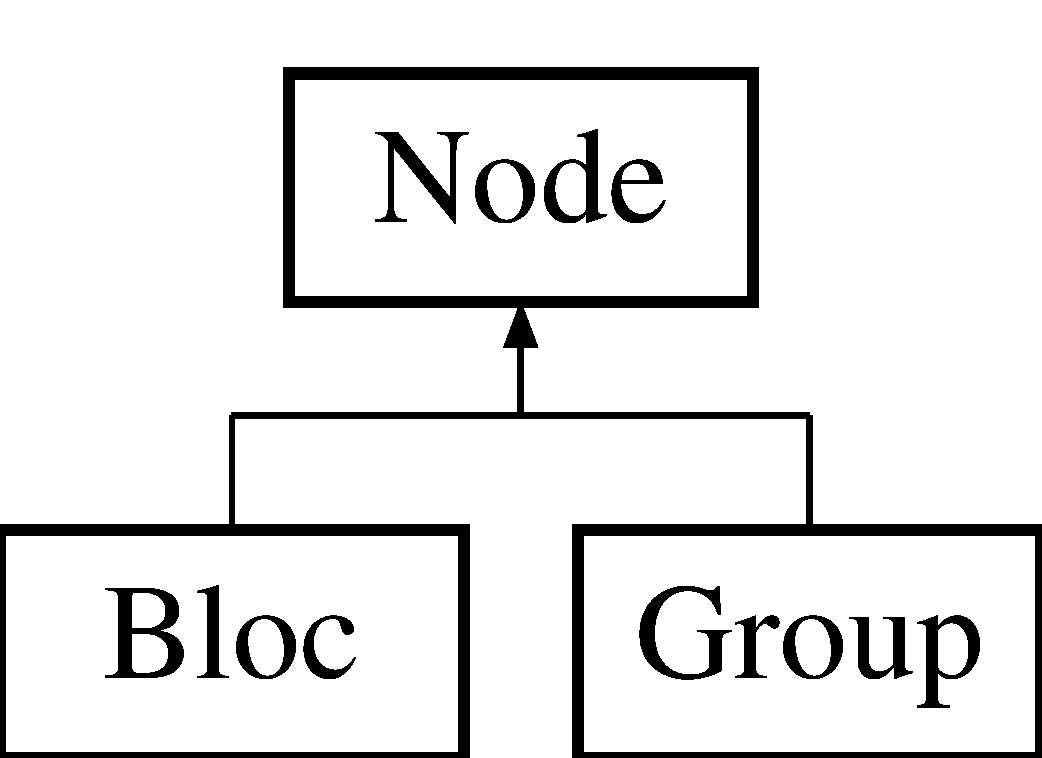
\includegraphics[height=2.000000cm]{class_open_chams_1_1_node}
\end{center}
\end{figure}
\subsection*{Public Member Functions}
\begin{DoxyCompactItemize}
\item 
\mbox{\Hypertarget{class_open_chams_1_1_node_a3fd7335faa33dce2f87c7e50eef3e294}\label{class_open_chams_1_1_node_a3fd7335faa33dce2f87c7e50eef3e294}} 
const std\+::string \& \hyperlink{class_open_chams_1_1_node_a3fd7335faa33dce2f87c7e50eef3e294}{get\+Name} () const
\begin{DoxyCompactList}\small\item\em returns the name of the node. \end{DoxyCompactList}\item 
\mbox{\Hypertarget{class_open_chams_1_1_node_afa302489ba7f4c55c5de696773c3d57b}\label{class_open_chams_1_1_node_afa302489ba7f4c55c5de696773c3d57b}} 
\hyperlink{class_open_chams_1_1_node}{Node} $\ast$ \hyperlink{class_open_chams_1_1_node_afa302489ba7f4c55c5de696773c3d57b}{get\+Parent} ()
\begin{DoxyCompactList}\small\item\em returns the parent node of the current node. \end{DoxyCompactList}\item 
\mbox{\Hypertarget{class_open_chams_1_1_node_a566f4d0bebb46cfd31384a8394a7dbb9}\label{class_open_chams_1_1_node_a566f4d0bebb46cfd31384a8394a7dbb9}} 
Position \hyperlink{class_open_chams_1_1_node_a566f4d0bebb46cfd31384a8394a7dbb9}{get\+Position} () const
\begin{DoxyCompactList}\small\item\em returns the position of the node. \end{DoxyCompactList}\item 
\mbox{\Hypertarget{class_open_chams_1_1_node_a9533ddcf078ddfc2a4e9bd9ffafa51cb}\label{class_open_chams_1_1_node_a9533ddcf078ddfc2a4e9bd9ffafa51cb}} 
\hyperlink{class_open_chams_1_1_node}{Node} $\ast$ \hyperlink{class_open_chams_1_1_node_a9533ddcf078ddfc2a4e9bd9ffafa51cb}{get\+Right} ()
\begin{DoxyCompactList}\small\item\em returns the child node at the right of the current node. \end{DoxyCompactList}\item 
\mbox{\Hypertarget{class_open_chams_1_1_node_af59967a8c2d5a04ca0a58e2ef29bead1}\label{class_open_chams_1_1_node_af59967a8c2d5a04ca0a58e2ef29bead1}} 
\hyperlink{class_open_chams_1_1_node}{Node} $\ast$ \hyperlink{class_open_chams_1_1_node_af59967a8c2d5a04ca0a58e2ef29bead1}{get\+Top} ()
\begin{DoxyCompactList}\small\item\em returns the child node at the top of the current node. \end{DoxyCompactList}\item 
\mbox{\Hypertarget{class_open_chams_1_1_node_ad78e3dab6fc481769907b77419fe4bac}\label{class_open_chams_1_1_node_ad78e3dab6fc481769907b77419fe4bac}} 
bool \hyperlink{class_open_chams_1_1_node_ad78e3dab6fc481769907b77419fe4bac}{is\+Root} ()
\begin{DoxyCompactList}\small\item\em returns tru if the node is the root of the tree (has no parent). \end{DoxyCompactList}\item 
void \hyperlink{class_open_chams_1_1_node_a55d8fa1d2b1c961fcab18acbf67c8be1}{set\+Right} (\hyperlink{class_open_chams_1_1_node}{Node} $\ast$)
\begin{DoxyCompactList}\small\item\em sets the child node at the right of the current node. \end{DoxyCompactList}\item 
void \hyperlink{class_open_chams_1_1_node_a32e2fbbb73c6b7ee4a30189cc30106bf}{set\+Top} (\hyperlink{class_open_chams_1_1_node}{Node} $\ast$)
\begin{DoxyCompactList}\small\item\em sets the node at the top of the current node. \end{DoxyCompactList}\end{DoxyCompactItemize}


\subsection{Detailed Description}
This class describes a node of the placement tree.

This is an abstract class used to easily managed blocs and groups of the placement tree. 

\subsection{Member Function Documentation}
\mbox{\Hypertarget{class_open_chams_1_1_node_a55d8fa1d2b1c961fcab18acbf67c8be1}\label{class_open_chams_1_1_node_a55d8fa1d2b1c961fcab18acbf67c8be1}} 
\index{Open\+Chams\+::\+Node@{Open\+Chams\+::\+Node}!set\+Right@{set\+Right}}
\index{set\+Right@{set\+Right}!Open\+Chams\+::\+Node@{Open\+Chams\+::\+Node}}
\subsubsection{\texorpdfstring{set\+Right()}{setRight()}}
{\footnotesize\ttfamily void set\+Right (\begin{DoxyParamCaption}\item[{\hyperlink{class_open_chams_1_1_node}{Node} $\ast$}]{node }\end{DoxyParamCaption})\hspace{0.3cm}{\ttfamily [inline]}}



sets the child node at the right of the current node. 


\begin{DoxyParams}{Parameters}
{\em node} & the node at the right of the current node. \\
\hline
\end{DoxyParams}
\mbox{\Hypertarget{class_open_chams_1_1_node_a32e2fbbb73c6b7ee4a30189cc30106bf}\label{class_open_chams_1_1_node_a32e2fbbb73c6b7ee4a30189cc30106bf}} 
\index{Open\+Chams\+::\+Node@{Open\+Chams\+::\+Node}!set\+Top@{set\+Top}}
\index{set\+Top@{set\+Top}!Open\+Chams\+::\+Node@{Open\+Chams\+::\+Node}}
\subsubsection{\texorpdfstring{set\+Top()}{setTop()}}
{\footnotesize\ttfamily void set\+Top (\begin{DoxyParamCaption}\item[{\hyperlink{class_open_chams_1_1_node}{Node} $\ast$}]{node }\end{DoxyParamCaption})\hspace{0.3cm}{\ttfamily [inline]}}



sets the node at the top of the current node. 


\begin{DoxyParams}{Parameters}
{\em node} & the node at the top of the current node. \\
\hline
\end{DoxyParams}

\hypertarget{class_open_chams_1_1_n_r_c_cstr}{\section{N\-R\-C\-Cstr Class Reference}
\label{class_open_chams_1_1_n_r_c_cstr}\index{N\-R\-C\-Cstr@{N\-R\-C\-Cstr}}
}
Inheritance diagram for N\-R\-C\-Cstr\-:\begin{figure}[H]
\begin{center}
\leavevmode
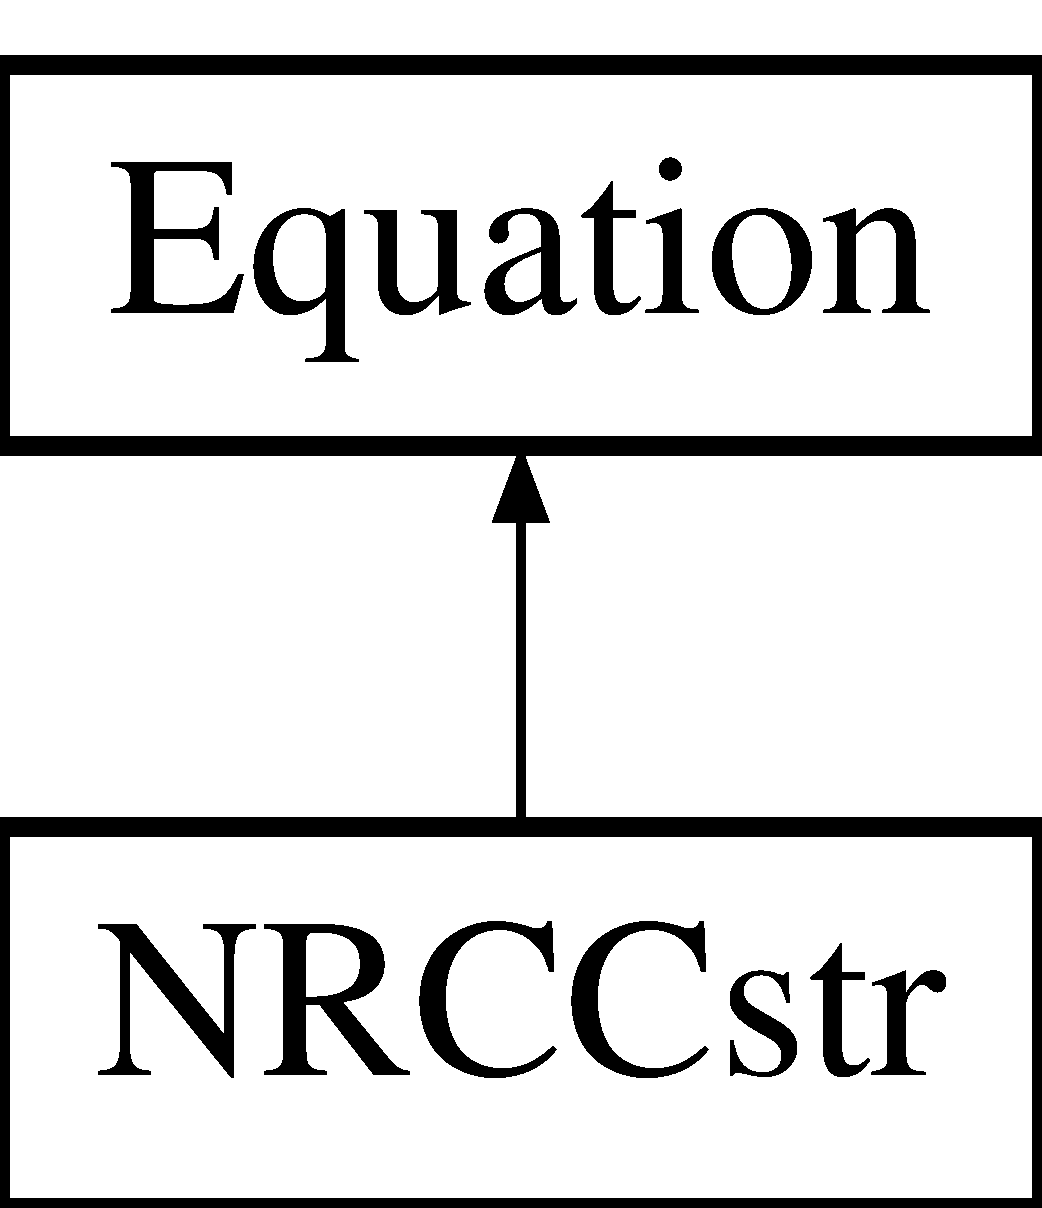
\includegraphics[height=2.000000cm]{class_open_chams_1_1_n_r_c_cstr}
\end{center}
\end{figure}

\hypertarget{class_open_chams_1_1_open_chams_exception}{}\section{Open\+Chams\+Exception Class Reference}
\label{class_open_chams_1_1_open_chams_exception}\index{Open\+Chams\+Exception@{Open\+Chams\+Exception}}


\subsection{Detailed Description}
This class describes the exceptions throwed by the Open\+Chams library in case of errors. 
\hypertarget{class_open_chams_1_1_operator}{}\section{Operator Class Reference}
\label{class_open_chams_1_1_operator}\index{Operator@{Operator}}
\subsection*{Data Structures}
\begin{DoxyCompactItemize}
\item 
class \hyperlink{class_open_chams_1_1_operator_1_1_constraint}{Constraint}
\end{DoxyCompactItemize}
\subsection*{Public Member Functions}
\begin{DoxyCompactItemize}
\item 
\mbox{\Hypertarget{class_open_chams_1_1_operator_a0002889b395185948d7c71b261343620}\label{class_open_chams_1_1_operator_a0002889b395185948d7c71b261343620}} 
const std\+::map$<$ std\+::string, \hyperlink{class_open_chams_1_1_operator_1_1_constraint}{Constraint} $\ast$ $>$ \& \hyperlink{class_open_chams_1_1_operator_a0002889b395185948d7c71b261343620}{get\+Constraints} ()
\begin{DoxyCompactList}\small\item\em returns the map of operator\textquotesingle{}s constraints. \end{DoxyCompactList}\item 
\mbox{\Hypertarget{class_open_chams_1_1_operator_a2858c0c4e8b5108f041237cf5a802029}\label{class_open_chams_1_1_operator_a2858c0c4e8b5108f041237cf5a802029}} 
const std\+::string \& \hyperlink{class_open_chams_1_1_operator_a2858c0c4e8b5108f041237cf5a802029}{get\+Name} ()
\begin{DoxyCompactList}\small\item\em returns the name of the operator. \end{DoxyCompactList}\item 
\mbox{\Hypertarget{class_open_chams_1_1_operator_aa189a1b119b44a8877c478e2d2357a89}\label{class_open_chams_1_1_operator_aa189a1b119b44a8877c478e2d2357a89}} 
const std\+::string \& \hyperlink{class_open_chams_1_1_operator_aa189a1b119b44a8877c478e2d2357a89}{get\+Simul\+Model} ()
\begin{DoxyCompactList}\small\item\em returns the \hyperlink{class_open_chams_1_1_simul_model}{Simul\+Model} of the operator. \end{DoxyCompactList}\item 
\mbox{\Hypertarget{class_open_chams_1_1_operator_a9ac68ad3e43b1649a8582c8685f4886d}\label{class_open_chams_1_1_operator_a9ac68ad3e43b1649a8582c8685f4886d}} 
bool \hyperlink{class_open_chams_1_1_operator_a9ac68ad3e43b1649a8582c8685f4886d}{has\+No\+Constraints} ()
\begin{DoxyCompactList}\small\item\em returns true if operator has no \hyperlink{class_open_chams_1_1_operator_1_1_constraint}{Constraint}. \end{DoxyCompactList}\item 
\hyperlink{class_open_chams_1_1_operator_a9e0a20318f4b2d91498f82b90504f2af}{Operator} (const std\+::string \&operator\+Name, const std\+::string \&simul\+Model)
\begin{DoxyCompactList}\small\item\em creates a new operator. \end{DoxyCompactList}\end{DoxyCompactItemize}


\subsection{Detailed Description}
This class describes an operator of a sizing procedure. 

\subsection{Constructor \& Destructor Documentation}
\mbox{\Hypertarget{class_open_chams_1_1_operator_a9e0a20318f4b2d91498f82b90504f2af}\label{class_open_chams_1_1_operator_a9e0a20318f4b2d91498f82b90504f2af}} 
\index{Open\+Chams\+::\+Operator@{Open\+Chams\+::\+Operator}!Operator@{Operator}}
\index{Operator@{Operator}!Open\+Chams\+::\+Operator@{Open\+Chams\+::\+Operator}}
\subsubsection{\texorpdfstring{Operator()}{Operator()}}
{\footnotesize\ttfamily \hyperlink{class_open_chams_1_1_operator}{Operator} (\begin{DoxyParamCaption}\item[{const std\+::string \&}]{operator\+Name,  }\item[{const std\+::string \&}]{simul\+Model }\end{DoxyParamCaption})}



creates a new operator. 


\begin{DoxyParams}{Parameters}
{\em name} & the name of the operator. \\
\hline
{\em simul\+Model} & the simulation model of the operator. \\
\hline
{\em call\+Order} & the call order of the operator in the sizing procedure. \\
\hline
\end{DoxyParams}

\hypertarget{class_open_chams_1_1_parameters}{}\section{Parameters Class Reference}
\label{class_open_chams_1_1_parameters}\index{Parameters@{Parameters}}
\subsection*{Public Member Functions}
\begin{DoxyCompactItemize}
\item 
void \mbox{\hyperlink{class_open_chams_1_1_parameters_a9ad9a7acc15a142788270ccd255b5e91}{add\+Parameter}} (const std\+::string \&, const std\+::string \&)
\begin{DoxyCompactList}\small\item\em adds a new value parameter. \end{DoxyCompactList}\item 
const std\+::string \& \mbox{\hyperlink{class_open_chams_1_1_parameters_a41b343d6037f531fd92912b453b40f2b}{get\+Value}} (const std\+::string \&)
\begin{DoxyCompactList}\small\item\em returns the value of the parameter named {\ttfamily name}. \end{DoxyCompactList}\item 
\mbox{\Hypertarget{class_open_chams_1_1_parameters_a0f890d16c3b2a0bcbdf060854ea07877}\label{class_open_chams_1_1_parameters_a0f890d16c3b2a0bcbdf060854ea07877}} 
const std\+::map$<$ std\+::string, std\+::string $>$ \& \mbox{\hyperlink{class_open_chams_1_1_parameters_a0f890d16c3b2a0bcbdf060854ea07877}{get\+Values}} ()
\begin{DoxyCompactList}\small\item\em returns the map of value parameters. \end{DoxyCompactList}\item 
\mbox{\Hypertarget{class_open_chams_1_1_parameters_af337ffd75e4f019ce15302c60715d84b}\label{class_open_chams_1_1_parameters_af337ffd75e4f019ce15302c60715d84b}} 
bool \mbox{\hyperlink{class_open_chams_1_1_parameters_af337ffd75e4f019ce15302c60715d84b}{is\+Empty}} ()
\begin{DoxyCompactList}\small\item\em returns true if \mbox{\hyperlink{class_open_chams_1_1_parameters}{Parameters}} has no value parameter nor equation parameter. \end{DoxyCompactList}\item 
\mbox{\Hypertarget{class_open_chams_1_1_parameters_a061bbedbf4fbd963871a388f5e8ebb61}\label{class_open_chams_1_1_parameters_a061bbedbf4fbd963871a388f5e8ebb61}} 
\mbox{\hyperlink{class_open_chams_1_1_parameters_a061bbedbf4fbd963871a388f5e8ebb61}{Parameters}} ()
\begin{DoxyCompactList}\small\item\em creates a new set of parameters. \end{DoxyCompactList}\end{DoxyCompactItemize}


\subsection{Detailed Description}
This class describes a set of \mbox{\hyperlink{class_open_chams_1_1_parameters}{Parameters}}. \mbox{\hyperlink{class_open_chams_1_1_parameters}{Parameters}} consist in two maps associating a parameter name to a double value or a std\+::string (equation). 

\subsection{Member Function Documentation}
\mbox{\Hypertarget{class_open_chams_1_1_parameters_a9ad9a7acc15a142788270ccd255b5e91}\label{class_open_chams_1_1_parameters_a9ad9a7acc15a142788270ccd255b5e91}} 
\index{Open\+Chams\+::\+Parameters@{Open\+Chams\+::\+Parameters}!add\+Parameter@{add\+Parameter}}
\index{add\+Parameter@{add\+Parameter}!Open\+Chams\+::\+Parameters@{Open\+Chams\+::\+Parameters}}
\subsubsection{\texorpdfstring{add\+Parameter()}{addParameter()}}
{\footnotesize\ttfamily void add\+Parameter (\begin{DoxyParamCaption}\item[{const std\+::string \&}]{name,  }\item[{const std\+::string \&}]{value }\end{DoxyParamCaption})}



adds a new value parameter. 

adds a new equation parameter.


\begin{DoxyParams}{Parameters}
{\em name} & the name of the parameter. \\
\hline
{\em value} & the value of the parameter.\\
\hline
{\em name} & the name of the parameter. \\
\hline
{\em equation} & the equation of the parameter. \\
\hline
\end{DoxyParams}
\mbox{\Hypertarget{class_open_chams_1_1_parameters_a41b343d6037f531fd92912b453b40f2b}\label{class_open_chams_1_1_parameters_a41b343d6037f531fd92912b453b40f2b}} 
\index{Open\+Chams\+::\+Parameters@{Open\+Chams\+::\+Parameters}!get\+Value@{get\+Value}}
\index{get\+Value@{get\+Value}!Open\+Chams\+::\+Parameters@{Open\+Chams\+::\+Parameters}}
\subsubsection{\texorpdfstring{get\+Value()}{getValue()}}
{\footnotesize\ttfamily const string \& get\+Value (\begin{DoxyParamCaption}\item[{const std\+::string \&}]{name }\end{DoxyParamCaption})}



returns the value of the parameter named {\ttfamily name}. 


\begin{DoxyParams}{Parameters}
{\em name} & the name of the parameter.\\
\hline
\end{DoxyParams}
\begin{DoxyReturn}{Returns}
the parameter double value. 
\end{DoxyReturn}

\hypertarget{class_c_i_f_1_1_polygon}{}\section{Polygon Class Reference}
\label{class_c_i_f_1_1_polygon}\index{Polygon@{Polygon}}
\subsection*{Public Member Functions}
\begin{DoxyCompactItemize}
\item 
void \mbox{\hyperlink{class_c_i_f_1_1_polygon_ab3047469780327f18539907e1303ea15}{add\+Point}} (long, long)
\begin{DoxyCompactList}\small\item\em adds a point to the polygon. \end{DoxyCompactList}\item 
\mbox{\hyperlink{class_c_i_f_1_1_polygon_a07683a8a7dea6f09aba6997cc99fff5a}{Polygon}} (long)
\begin{DoxyCompactList}\small\item\em creates a new \mbox{\hyperlink{class_c_i_f_1_1_polygon}{Polygon}}. \end{DoxyCompactList}\end{DoxyCompactItemize}


\subsection{Detailed Description}
This class describes a polygon shape, which consists in a set of points (ie (x,y) pair). 

\subsection{Constructor \& Destructor Documentation}
\mbox{\Hypertarget{class_c_i_f_1_1_polygon_a07683a8a7dea6f09aba6997cc99fff5a}\label{class_c_i_f_1_1_polygon_a07683a8a7dea6f09aba6997cc99fff5a}} 
\index{C\+I\+F\+::\+Polygon@{C\+I\+F\+::\+Polygon}!Polygon@{Polygon}}
\index{Polygon@{Polygon}!C\+I\+F\+::\+Polygon@{C\+I\+F\+::\+Polygon}}
\subsubsection{\texorpdfstring{Polygon()}{Polygon()}}
{\footnotesize\ttfamily \mbox{\hyperlink{class_c_i_f_1_1_polygon}{Polygon}} (\begin{DoxyParamCaption}\item[{long}]{layer }\end{DoxyParamCaption})}



creates a new \mbox{\hyperlink{class_c_i_f_1_1_polygon}{Polygon}}. 


\begin{DoxyParams}{Parameters}
{\em layer} & the layer on which the polygon is created. \\
\hline
\end{DoxyParams}


\subsection{Member Function Documentation}
\mbox{\Hypertarget{class_c_i_f_1_1_polygon_ab3047469780327f18539907e1303ea15}\label{class_c_i_f_1_1_polygon_ab3047469780327f18539907e1303ea15}} 
\index{C\+I\+F\+::\+Polygon@{C\+I\+F\+::\+Polygon}!add\+Point@{add\+Point}}
\index{add\+Point@{add\+Point}!C\+I\+F\+::\+Polygon@{C\+I\+F\+::\+Polygon}}
\subsubsection{\texorpdfstring{add\+Point()}{addPoint()}}
{\footnotesize\ttfamily void add\+Point (\begin{DoxyParamCaption}\item[{long}]{x,  }\item[{long}]{y }\end{DoxyParamCaption})}



adds a point to the polygon. 


\begin{DoxyParams}{Parameters}
{\em x} & the x coordinate of the point. \\
\hline
{\em y} & the y coordinate of the point. \\
\hline
\end{DoxyParams}

\hypertarget{class_open_chams_1_1_port}{}\section{Port Class Reference}
\label{class_open_chams_1_1_port}\index{Port@{Port}}
\subsection*{Public Member Functions}
\begin{DoxyCompactItemize}
\item 
\mbox{\Hypertarget{class_open_chams_1_1_port_a743f20da85b9a06d9984c0adc337afc1}\label{class_open_chams_1_1_port_a743f20da85b9a06d9984c0adc337afc1}} 
unsigned \hyperlink{class_open_chams_1_1_port_a743f20da85b9a06d9984c0adc337afc1}{get\+Index} () const
\begin{DoxyCompactList}\small\item\em returns the index of the port. \end{DoxyCompactList}\item 
\mbox{\Hypertarget{class_open_chams_1_1_port_ace51e4bf9cee0319600c14723efa0dfb}\label{class_open_chams_1_1_port_ace51e4bf9cee0319600c14723efa0dfb}} 
const std\+::string \& \hyperlink{class_open_chams_1_1_port_ace51e4bf9cee0319600c14723efa0dfb}{get\+Orientation} () const
\begin{DoxyCompactList}\small\item\em returns the orientation of the port. \end{DoxyCompactList}\item 
\mbox{\Hypertarget{class_open_chams_1_1_port_a49fc4eb493558cf55dd00df9ef5f8f08}\label{class_open_chams_1_1_port_a49fc4eb493558cf55dd00df9ef5f8f08}} 
const std\+::string \& \hyperlink{class_open_chams_1_1_port_a49fc4eb493558cf55dd00df9ef5f8f08}{get\+Type} () const
\begin{DoxyCompactList}\small\item\em returns the type of the port. \end{DoxyCompactList}\item 
\mbox{\Hypertarget{class_open_chams_1_1_port_a344385751bee0720059403940d57a13e}\label{class_open_chams_1_1_port_a344385751bee0720059403940d57a13e}} 
double \hyperlink{class_open_chams_1_1_port_a344385751bee0720059403940d57a13e}{getX} () const
\begin{DoxyCompactList}\small\item\em returns the x coordinate of the port. \end{DoxyCompactList}\item 
\mbox{\Hypertarget{class_open_chams_1_1_port_aafa51c7f8f38a09febbb9ce7853f77b4}\label{class_open_chams_1_1_port_aafa51c7f8f38a09febbb9ce7853f77b4}} 
double \hyperlink{class_open_chams_1_1_port_aafa51c7f8f38a09febbb9ce7853f77b4}{getY} () const
\begin{DoxyCompactList}\small\item\em returns the y coordinate of the port. \end{DoxyCompactList}\item 
\hyperlink{class_open_chams_1_1_port_ab13daf22aea531e874ff42a71b49a112}{Port} (const std\+::string \&type, unsigned idx, double x, double y, const std\+::string \&orient)
\begin{DoxyCompactList}\small\item\em creates a new port. \end{DoxyCompactList}\end{DoxyCompactItemize}


\subsection{Detailed Description}
This class describes port.

A port is used by schematic to position the input/output ports of the circuit.

\begin{DoxyNote}{Note}
Althought the \hyperlink{class_open_chams_1_1_port}{Port} object is related to \hyperlink{class_open_chams_1_1_schematic}{Schematic}, it is handled by \hyperlink{class_open_chams_1_1_net}{Net} object since a port always belongs to a \hyperlink{class_open_chams_1_1_net}{Net}. 
\end{DoxyNote}


\subsection{Constructor \& Destructor Documentation}
\mbox{\Hypertarget{class_open_chams_1_1_port_ab13daf22aea531e874ff42a71b49a112}\label{class_open_chams_1_1_port_ab13daf22aea531e874ff42a71b49a112}} 
\index{Open\+Chams\+::\+Port@{Open\+Chams\+::\+Port}!Port@{Port}}
\index{Port@{Port}!Open\+Chams\+::\+Port@{Open\+Chams\+::\+Port}}
\subsubsection{\texorpdfstring{Port()}{Port()}}
{\footnotesize\ttfamily \hyperlink{class_open_chams_1_1_port}{Port} (\begin{DoxyParamCaption}\item[{const std\+::string \&}]{type,  }\item[{unsigned}]{idx,  }\item[{double}]{x,  }\item[{double}]{y,  }\item[{const std\+::string \&}]{orient }\end{DoxyParamCaption})\hspace{0.3cm}{\ttfamily [inline]}}



creates a new port. 


\begin{DoxyParams}{Parameters}
{\em type} & the type of the port. \\
\hline
{\em idx} & the index of the port (index of nets belonging to the same net must be different). \\
\hline
{\em x} & the x coordinate of the port. \\
\hline
{\em y} & the y coordinate of the port. \\
\hline
{\em orient} & the orientation of the port. \\
\hline
\end{DoxyParams}

\hypertarget{class_open_chams_1_1_port_point}{\section{Port\-Point Class Reference}
\label{class_open_chams_1_1_port_point}\index{Port\-Point@{Port\-Point}}
}
Inheritance diagram for Port\-Point\-:\begin{figure}[H]
\begin{center}
\leavevmode
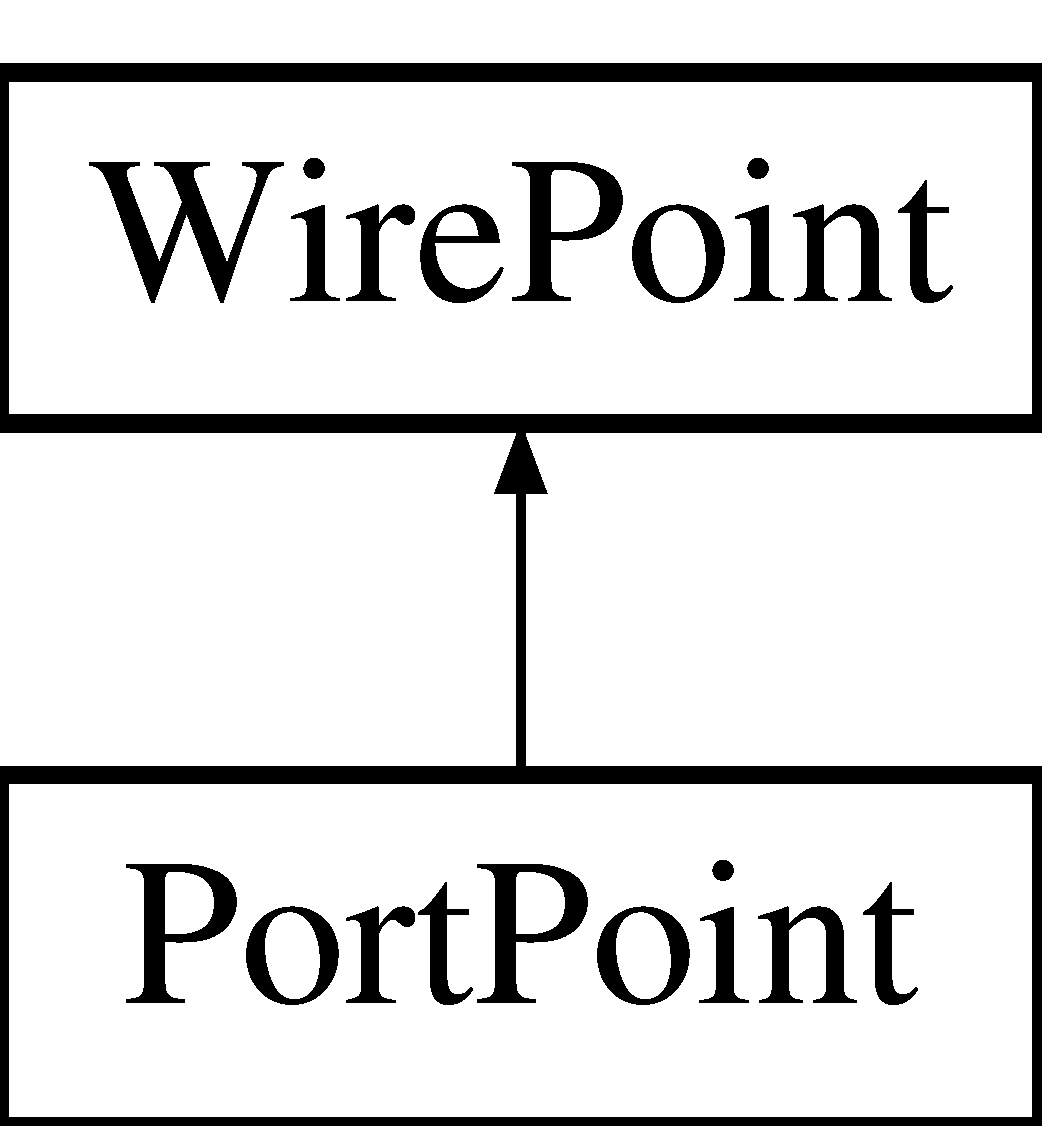
\includegraphics[height=2.000000cm]{class_open_chams_1_1_port_point}
\end{center}
\end{figure}
\subsection*{Public Member Functions}
\begin{DoxyCompactItemize}
\item 
\hypertarget{class_open_chams_1_1_port_point_ab4018980dcd1fed5208e7a72846cd815}{unsigned \hyperlink{class_open_chams_1_1_port_point_ab4018980dcd1fed5208e7a72846cd815}{get\-Index} ()}\label{class_open_chams_1_1_port_point_ab4018980dcd1fed5208e7a72846cd815}

\begin{DoxyCompactList}\small\item\em returns the index of the port associated to the port\-Point. \end{DoxyCompactList}\item 
\hyperlink{class_open_chams_1_1_port_point_aaa11e5ede2581539ec666941e1c86fc3}{Port\-Point} (unsigned idx)
\begin{DoxyCompactList}\small\item\em creates a new wire point associated to a port. \end{DoxyCompactList}\end{DoxyCompactItemize}


\subsection{Detailed Description}
this class describes a wire point associated to a \hyperlink{class_open_chams_1_1_port}{Port}. 

\subsection{Constructor \& Destructor Documentation}
\hypertarget{class_open_chams_1_1_port_point_aaa11e5ede2581539ec666941e1c86fc3}{\index{Open\-Chams\-::\-Port\-Point@{Open\-Chams\-::\-Port\-Point}!Port\-Point@{Port\-Point}}
\index{Port\-Point@{Port\-Point}!OpenChams::PortPoint@{Open\-Chams\-::\-Port\-Point}}
\subsubsection[{Port\-Point}]{\setlength{\rightskip}{0pt plus 5cm}{\bf Port\-Point} (
\begin{DoxyParamCaption}
\item[{unsigned}]{idx}
\end{DoxyParamCaption}
)\hspace{0.3cm}{\ttfamily [inline]}}}\label{class_open_chams_1_1_port_point_aaa11e5ede2581539ec666941e1c86fc3}


creates a new wire point associated to a port. 


\begin{DoxyParams}{Parameters}
{\em idx} & the index of the port associated to the port\-Point.\\
\hline
\end{DoxyParams}
\begin{DoxyNote}{Note}
The index of the port is only valid considering the net to which the wire is relative. 
\end{DoxyNote}

\hypertarget{class_a_g_d_s_1_1_rectangle}{}\section{Rectangle Class Reference}
\label{class_a_g_d_s_1_1_rectangle}\index{Rectangle@{Rectangle}}
Inheritance diagram for Rectangle\+:\begin{figure}[H]
\begin{center}
\leavevmode
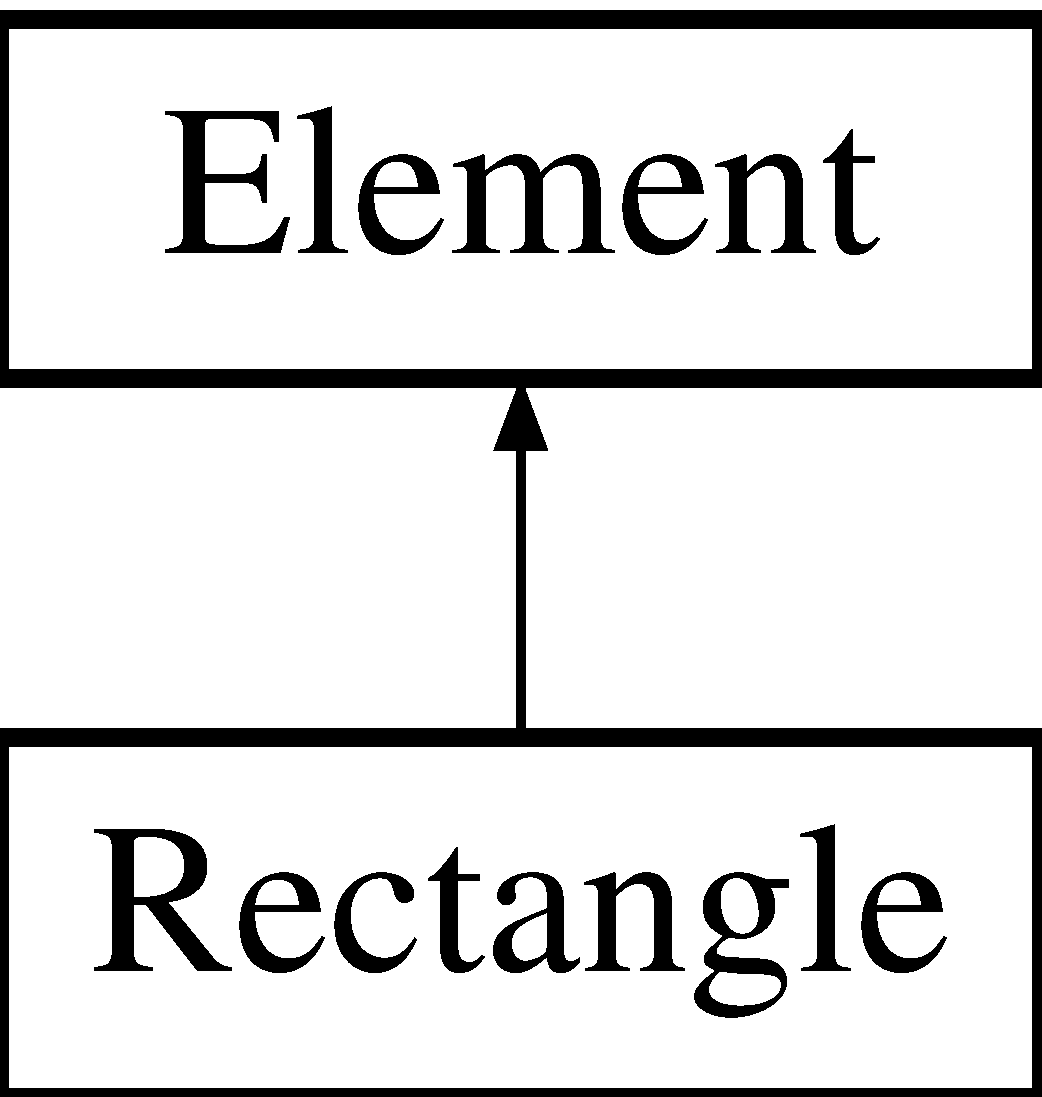
\includegraphics[height=2.000000cm]{class_a_g_d_s_1_1_rectangle}
\end{center}
\end{figure}
\subsection*{Public Member Functions}
\begin{DoxyCompactItemize}
\item 
\hyperlink{class_a_g_d_s_1_1_rectangle_a84899edb51e65c78535f0b06b266f11b}{Rectangle} (int layer, double xmin, double ymin, double xmax, double ymax)
\begin{DoxyCompactList}\small\item\em creates a new \hyperlink{class_a_g_d_s_1_1_rectangle}{Rectangle} \end{DoxyCompactList}\end{DoxyCompactItemize}


\subsection{Detailed Description}
This class describes a rectangle element and inherits from \hyperlink{class_a_g_d_s_1_1_element}{A\+G\+D\+S\+::\+Element}. 

\subsection{Constructor \& Destructor Documentation}
\mbox{\Hypertarget{class_a_g_d_s_1_1_rectangle_a84899edb51e65c78535f0b06b266f11b}\label{class_a_g_d_s_1_1_rectangle_a84899edb51e65c78535f0b06b266f11b}} 
\index{A\+G\+D\+S\+::\+Rectangle@{A\+G\+D\+S\+::\+Rectangle}!Rectangle@{Rectangle}}
\index{Rectangle@{Rectangle}!A\+G\+D\+S\+::\+Rectangle@{A\+G\+D\+S\+::\+Rectangle}}
\subsubsection{\texorpdfstring{Rectangle()}{Rectangle()}}
{\footnotesize\ttfamily \hyperlink{class_a_g_d_s_1_1_rectangle}{Rectangle} (\begin{DoxyParamCaption}\item[{int}]{layer,  }\item[{double}]{xmin,  }\item[{double}]{ymin,  }\item[{double}]{xmax,  }\item[{double}]{ymax }\end{DoxyParamCaption})}



creates a new \hyperlink{class_a_g_d_s_1_1_rectangle}{Rectangle} 


\begin{DoxyParams}{Parameters}
{\em layer} & the layer number into which the rectangle shape is drawned. \\
\hline
{\em xmin} & the x coordinate of the bottom-\/left corner of the rectangle. \\
\hline
{\em ymin} & the y coordinate of the bottom-\/left corner of the rectangle. \\
\hline
{\em xmax} & the x coordinate of the top-\/right corner of the rectangle. \\
\hline
{\em ymax} & the y coordinate of the top-\/right corner of the rectangle. \\
\hline
\end{DoxyParams}

\hypertarget{class_s_p_i_c_e_1_1_resistor}{}\section{Resistor Class Reference}
\label{class_s_p_i_c_e_1_1_resistor}\index{Resistor@{Resistor}}
Inheritance diagram for Resistor\+:\begin{figure}[H]
\begin{center}
\leavevmode
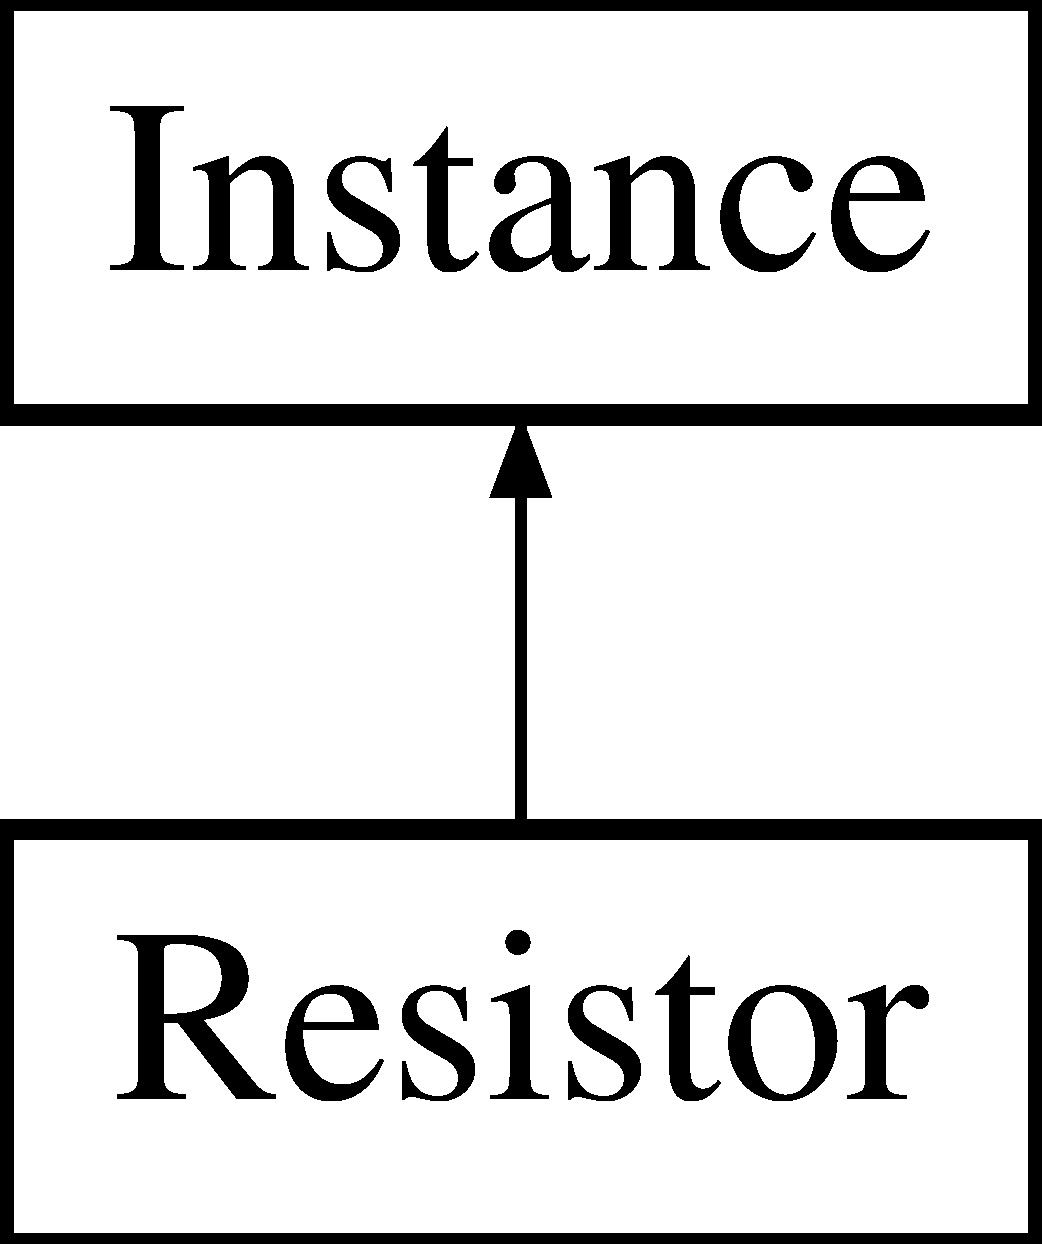
\includegraphics[height=2.000000cm]{class_s_p_i_c_e_1_1_resistor}
\end{center}
\end{figure}
\subsection*{Public Member Functions}
\begin{DoxyCompactItemize}
\item 
\mbox{\Hypertarget{class_s_p_i_c_e_1_1_resistor_ab57aa52f48a5a56c89dd49eae66c1a0f}\label{class_s_p_i_c_e_1_1_resistor_ab57aa52f48a5a56c89dd49eae66c1a0f}} 
std\+::string \mbox{\hyperlink{class_s_p_i_c_e_1_1_resistor_ab57aa52f48a5a56c89dd49eae66c1a0f}{get\+First}} ()
\begin{DoxyCompactList}\small\item\em returns the first connector of the resistor. \end{DoxyCompactList}\item 
\mbox{\Hypertarget{class_s_p_i_c_e_1_1_resistor_a9665313821b2fca41e14b9865133af7f}\label{class_s_p_i_c_e_1_1_resistor_a9665313821b2fca41e14b9865133af7f}} 
std\+::string \mbox{\hyperlink{class_s_p_i_c_e_1_1_resistor_a9665313821b2fca41e14b9865133af7f}{get\+Second}} ()
\begin{DoxyCompactList}\small\item\em returns the second connector of the resistor. \end{DoxyCompactList}\item 
\mbox{\Hypertarget{class_s_p_i_c_e_1_1_resistor_a4c052cb2622c580a250b2c783a436882}\label{class_s_p_i_c_e_1_1_resistor_a4c052cb2622c580a250b2c783a436882}} 
std\+::string \mbox{\hyperlink{class_s_p_i_c_e_1_1_resistor_a4c052cb2622c580a250b2c783a436882}{get\+Value}} ()
\begin{DoxyCompactList}\small\item\em returns the value of the resistor. \end{DoxyCompactList}\item 
\mbox{\hyperlink{class_s_p_i_c_e_1_1_resistor_aa4e89fab1189113134e98edbb0c622bf}{Resistor}} (std\+::string name, std\+::string first, std\+::string second, std\+::string value)
\begin{DoxyCompactList}\small\item\em creates a new resistor. \end{DoxyCompactList}\end{DoxyCompactItemize}


\subsection{Detailed Description}
This class describes a resistor which is a specialized instance which has two connectors and a value. 

\subsection{Constructor \& Destructor Documentation}
\mbox{\Hypertarget{class_s_p_i_c_e_1_1_resistor_aa4e89fab1189113134e98edbb0c622bf}\label{class_s_p_i_c_e_1_1_resistor_aa4e89fab1189113134e98edbb0c622bf}} 
\index{S\+P\+I\+C\+E\+::\+Resistor@{S\+P\+I\+C\+E\+::\+Resistor}!Resistor@{Resistor}}
\index{Resistor@{Resistor}!S\+P\+I\+C\+E\+::\+Resistor@{S\+P\+I\+C\+E\+::\+Resistor}}
\subsubsection{\texorpdfstring{Resistor()}{Resistor()}}
{\footnotesize\ttfamily \mbox{\hyperlink{class_s_p_i_c_e_1_1_resistor}{Resistor}} (\begin{DoxyParamCaption}\item[{std\+::string}]{name,  }\item[{std\+::string}]{first,  }\item[{std\+::string}]{second,  }\item[{std\+::string}]{value }\end{DoxyParamCaption})\hspace{0.3cm}{\ttfamily [inline]}}



creates a new resistor. 


\begin{DoxyParams}{Parameters}
{\em name} & the name of the resistor. \\
\hline
{\em first} & the first connector of the resistor. \\
\hline
{\em second} & the second connector of the resistor. \\
\hline
{\em value} & the value of the resistor. \\
\hline
\end{DoxyParams}

\hypertarget{class_open_chams_1_1_r_slicing_node}{\section{R\-Slicing\-Node Class Reference}
\label{class_open_chams_1_1_r_slicing_node}\index{R\-Slicing\-Node@{R\-Slicing\-Node}}
}
Inheritance diagram for R\-Slicing\-Node\-:\begin{figure}[H]
\begin{center}
\leavevmode
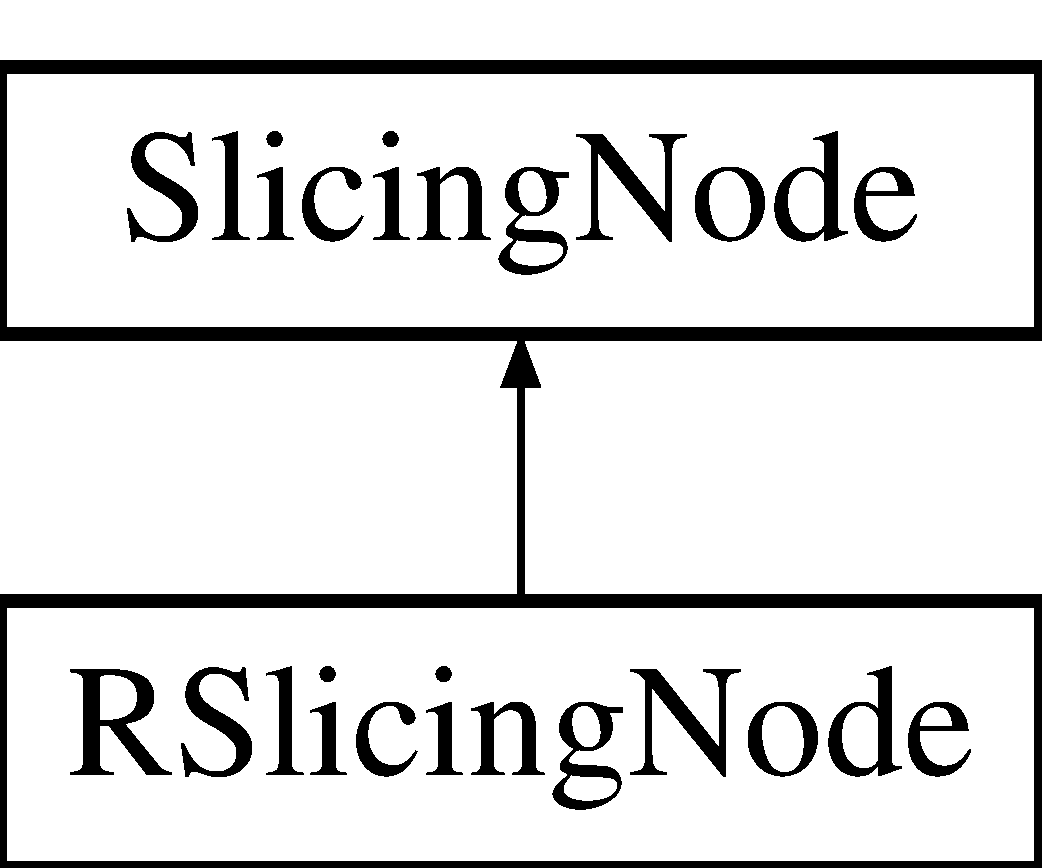
\includegraphics[height=2.000000cm]{class_open_chams_1_1_r_slicing_node}
\end{center}
\end{figure}

\hypertarget{class_d_t_r_1_1_rule}{}\section{Rule Class Reference}
\label{class_d_t_r_1_1_rule}\index{Rule@{Rule}}
Inheritance diagram for Rule\+:\begin{figure}[H]
\begin{center}
\leavevmode
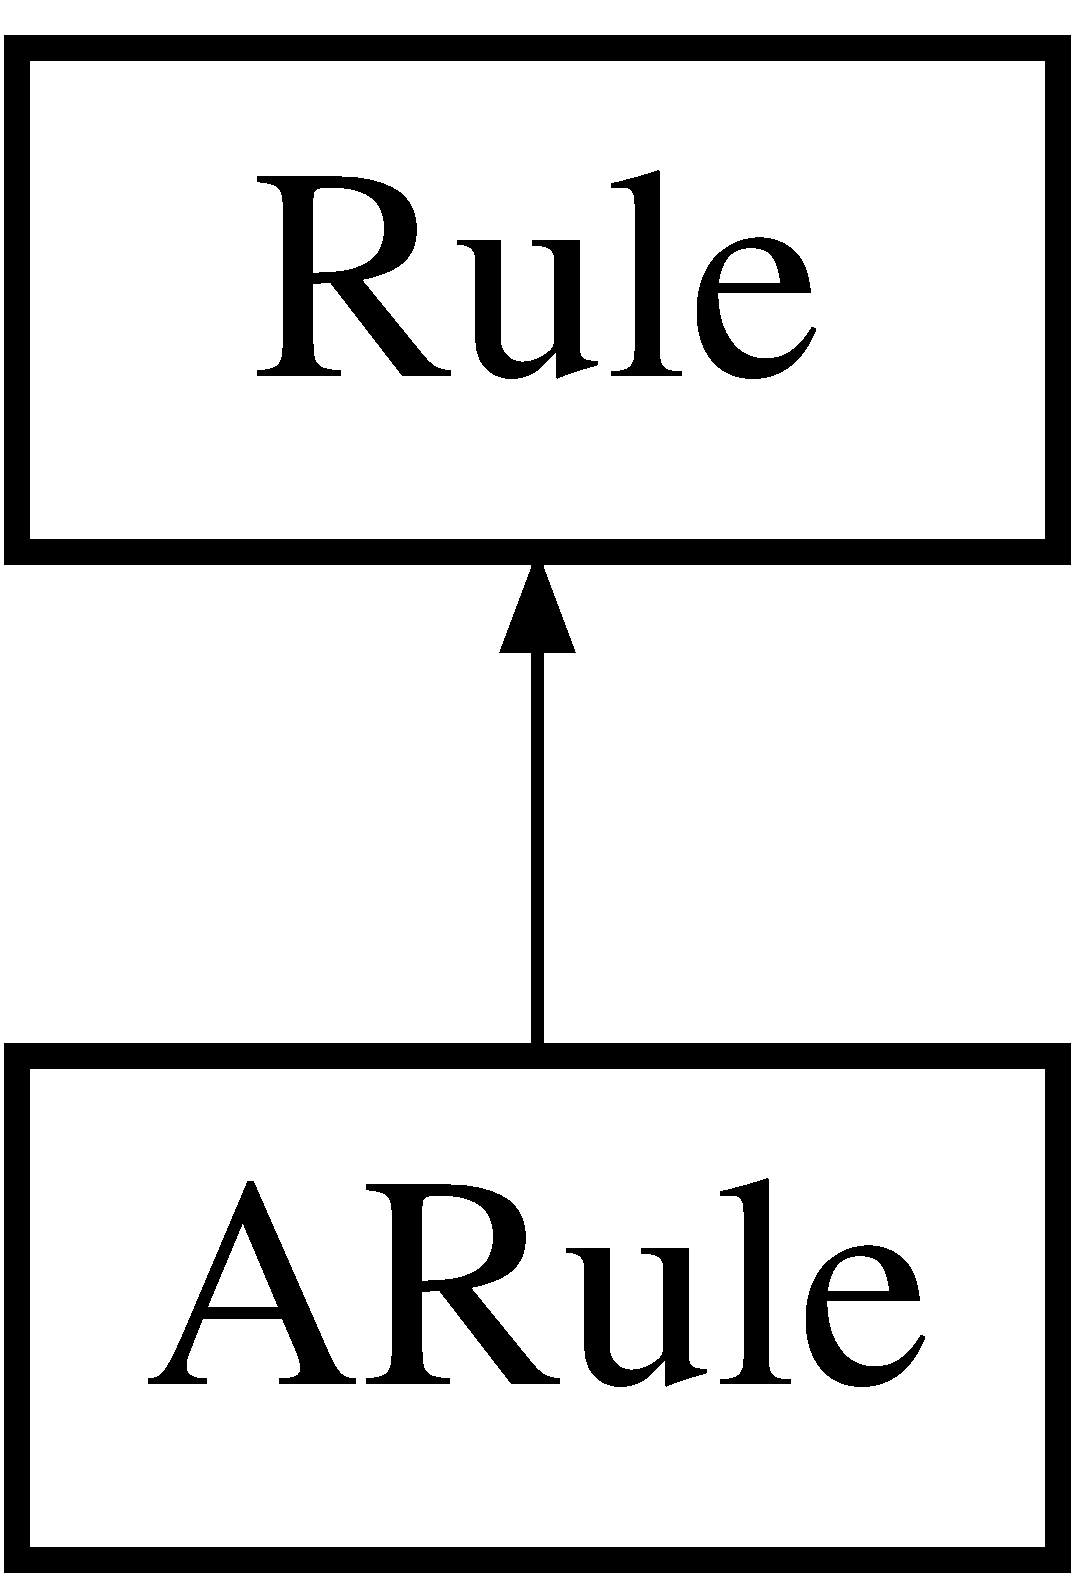
\includegraphics[height=2.000000cm]{class_d_t_r_1_1_rule}
\end{center}
\end{figure}
\subsection*{Public Member Functions}
\begin{DoxyCompactItemize}
\item 
\mbox{\Hypertarget{class_d_t_r_1_1_rule_a710e6d75d7ae8de075ced5da150e10db}\label{class_d_t_r_1_1_rule_a710e6d75d7ae8de075ced5da150e10db}} 
const std\+::string \& \mbox{\hyperlink{class_d_t_r_1_1_rule_a710e6d75d7ae8de075ced5da150e10db}{get\+Layer1}} ()
\begin{DoxyCompactList}\small\item\em returns the first layer of the rule. \end{DoxyCompactList}\item 
\mbox{\Hypertarget{class_d_t_r_1_1_rule_a29e6dc8d83450a582cbd9af372e96162}\label{class_d_t_r_1_1_rule_a29e6dc8d83450a582cbd9af372e96162}} 
virtual const std\+::string \& \mbox{\hyperlink{class_d_t_r_1_1_rule_a29e6dc8d83450a582cbd9af372e96162}{get\+Layer2}} ()
\begin{DoxyCompactList}\small\item\em returns the second layer of the rule. \end{DoxyCompactList}\item 
\mbox{\Hypertarget{class_d_t_r_1_1_rule_a2858c0c4e8b5108f041237cf5a802029}\label{class_d_t_r_1_1_rule_a2858c0c4e8b5108f041237cf5a802029}} 
const std\+::string \& \mbox{\hyperlink{class_d_t_r_1_1_rule_a2858c0c4e8b5108f041237cf5a802029}{get\+Name}} ()
\begin{DoxyCompactList}\small\item\em returns the name of the rule. \end{DoxyCompactList}\item 
\mbox{\Hypertarget{class_d_t_r_1_1_rule_a07cf74adaf661f0aaaa1818d24c2243d}\label{class_d_t_r_1_1_rule_a07cf74adaf661f0aaaa1818d24c2243d}} 
const std\+::string \& \mbox{\hyperlink{class_d_t_r_1_1_rule_a07cf74adaf661f0aaaa1818d24c2243d}{get\+Ref}} ()
\begin{DoxyCompactList}\small\item\em returns the reference of the rule. \end{DoxyCompactList}\item 
const std\+::string \& \mbox{\hyperlink{class_d_t_r_1_1_rule_a7a88ff26f0ba9cfbfa5059c565d1e30b}{get\+Type}} ()
\begin{DoxyCompactList}\small\item\em returns the type of the rule. \end{DoxyCompactList}\item 
\mbox{\Hypertarget{class_d_t_r_1_1_rule_a666f992950731c68de1ad441f80f228c}\label{class_d_t_r_1_1_rule_a666f992950731c68de1ad441f80f228c}} 
double \mbox{\hyperlink{class_d_t_r_1_1_rule_a666f992950731c68de1ad441f80f228c}{get\+Value}} ()
\begin{DoxyCompactList}\small\item\em returns the value of the rule. \end{DoxyCompactList}\item 
\mbox{\Hypertarget{class_d_t_r_1_1_rule_a3fad3e4886891e1efcdca530d2f6daa3}\label{class_d_t_r_1_1_rule_a3fad3e4886891e1efcdca530d2f6daa3}} 
const std\+::string \& \mbox{\hyperlink{class_d_t_r_1_1_rule_a3fad3e4886891e1efcdca530d2f6daa3}{get\+Value\+As\+String}} ()
\begin{DoxyCompactList}\small\item\em returns the string corresponding to the value of the rule. \end{DoxyCompactList}\item 
\mbox{\hyperlink{class_d_t_r_1_1_rule_aee8c5385eba121203f788a012b502e24}{Rule}} (const char $\ast$name, double value, const char $\ast$ref, const char $\ast$layer1, const char $\ast$layer2)
\begin{DoxyCompactList}\small\item\em creates a new rule. \end{DoxyCompactList}\item 
void \mbox{\hyperlink{class_d_t_r_1_1_rule_a3568407d7a7890c39b8c9acc1e608535}{set\+Type}} (const char $\ast$)
\begin{DoxyCompactList}\small\item\em sets the type of a rule. \end{DoxyCompactList}\end{DoxyCompactItemize}


\subsection{Detailed Description}
This class describes a symmetrical rule.

A symmetrical rule represents several type of rules\+:
\begin{DoxyItemize}
\item a simple rule with only a name (e.\+g. transistor\+MinW\+: transistor minimum width)
\item a rule for a unique layer (e.\+g. min\+Width.\+metal1\+: the minimum width for metal1 wire)
\item a rule associating two layers (e.\+g min\+Space.\+poly.\+active\+: the minimum spacing between a poly shape and an active shape) In this last case the symmetrical characteristic is important since it implies that the value is the same if we invert the two layers \+: min\+Spacing poly vs active = min\+Spacing active vs poly.
\end{DoxyItemize}

Typical rules using no layer are\+: {\itshape transistor\+MinW, transsitor\+MaxW, transistor\+MinL transistor\+MaxL}

Typical rules using one layer are\+: {\itshape min\+Width, min\+Spacing, min\+Area, min\+Gate\+Spacing, min\+Strap\+Enclosure}

Typical rules using two layers are\+: {\itshape min\+Spacing} 

\subsection{Constructor \& Destructor Documentation}
\mbox{\Hypertarget{class_d_t_r_1_1_rule_aee8c5385eba121203f788a012b502e24}\label{class_d_t_r_1_1_rule_aee8c5385eba121203f788a012b502e24}} 
\index{D\+T\+R\+::\+Rule@{D\+T\+R\+::\+Rule}!Rule@{Rule}}
\index{Rule@{Rule}!D\+T\+R\+::\+Rule@{D\+T\+R\+::\+Rule}}
\subsubsection{\texorpdfstring{Rule()}{Rule()}}
{\footnotesize\ttfamily \mbox{\hyperlink{class_d_t_r_1_1_rule}{Rule}} (\begin{DoxyParamCaption}\item[{const char $\ast$}]{name,  }\item[{double}]{value,  }\item[{const char $\ast$}]{ref,  }\item[{const char $\ast$}]{layer1,  }\item[{const char $\ast$}]{layer2 }\end{DoxyParamCaption})\hspace{0.3cm}{\ttfamily [inline]}}



creates a new rule. 


\begin{DoxyParams}{Parameters}
{\em name} & the name of the rule. \\
\hline
{\em value} & the value of the rule. \\
\hline
{\em ref} & the reference of the rule (helpful to find rule in design kit). \\
\hline
{\em layer1} & the first layer. \\
\hline
{\em layer2} & the second layer. \\
\hline
\end{DoxyParams}


\subsection{Member Function Documentation}
\mbox{\Hypertarget{class_d_t_r_1_1_rule_a7a88ff26f0ba9cfbfa5059c565d1e30b}\label{class_d_t_r_1_1_rule_a7a88ff26f0ba9cfbfa5059c565d1e30b}} 
\index{D\+T\+R\+::\+Rule@{D\+T\+R\+::\+Rule}!get\+Type@{get\+Type}}
\index{get\+Type@{get\+Type}!D\+T\+R\+::\+Rule@{D\+T\+R\+::\+Rule}}
\subsubsection{\texorpdfstring{get\+Type()}{getType()}}
{\footnotesize\ttfamily const std\+::string \& get\+Type (\begin{DoxyParamCaption}{ }\end{DoxyParamCaption})\hspace{0.3cm}{\ttfamily [inline]}}



returns the type of the rule. 

\mbox{\hyperlink{class_d_t_r_1_1_rule}{Rule}}\textquotesingle{}s type allows to set a specific type for a rule especially the \textquotesingle{}area\textquotesingle{} type to take into account that the value of the rule is to be considered in unit$^\wedge$2. \mbox{\Hypertarget{class_d_t_r_1_1_rule_a3568407d7a7890c39b8c9acc1e608535}\label{class_d_t_r_1_1_rule_a3568407d7a7890c39b8c9acc1e608535}} 
\index{D\+T\+R\+::\+Rule@{D\+T\+R\+::\+Rule}!set\+Type@{set\+Type}}
\index{set\+Type@{set\+Type}!D\+T\+R\+::\+Rule@{D\+T\+R\+::\+Rule}}
\subsubsection{\texorpdfstring{set\+Type()}{setType()}}
{\footnotesize\ttfamily void set\+Type (\begin{DoxyParamCaption}\item[{const char $\ast$}]{type }\end{DoxyParamCaption})\hspace{0.3cm}{\ttfamily [inline]}}



sets the type of a rule. 


\begin{DoxyParams}{Parameters}
{\em type} & the type of the rule.\\
\hline
\end{DoxyParams}
\begin{DoxyNote}{Note}
By default the type of a rule is \char`\"{}\char`\"{}. 
\end{DoxyNote}

\hypertarget{class_open_chams_1_1_schematic}{}\section{Schematic Class Reference}
\label{class_open_chams_1_1_schematic}\index{Schematic@{Schematic}}
\subsection*{Data Structures}
\begin{DoxyCompactItemize}
\item 
class \hyperlink{class_open_chams_1_1_schematic_1_1_infos}{Infos}
\end{DoxyCompactItemize}
\subsection*{Public Member Functions}
\begin{DoxyCompactItemize}
\item 
void \hyperlink{class_open_chams_1_1_schematic_ac7fc9f5cdf1e22c53d42e6606e1af8ef}{add\+Instance} (const std\+::string \&instance\+Name, double x, double y, const std\+::string \&orient)
\begin{DoxyCompactList}\small\item\em adds schematic informations for an instance. \end{DoxyCompactList}\item 
\mbox{\Hypertarget{class_open_chams_1_1_schematic_afa015b02922d82de9c44e8ffe8dc5d56}\label{class_open_chams_1_1_schematic_afa015b02922d82de9c44e8ffe8dc5d56}} 
const std\+::map$<$ std\+::string, \hyperlink{class_open_chams_1_1_schematic_1_1_infos}{Infos} $\ast$ $>$ \& \hyperlink{class_open_chams_1_1_schematic_afa015b02922d82de9c44e8ffe8dc5d56}{get\+Instances} ()
\begin{DoxyCompactList}\small\item\em returns the map of instance\textquotesingle{}s \hyperlink{class_open_chams_1_1_schematic_1_1_infos}{Infos}. \end{DoxyCompactList}\item 
\mbox{\Hypertarget{class_open_chams_1_1_schematic_adab62a25face462baec9a7fffb2b6158}\label{class_open_chams_1_1_schematic_adab62a25face462baec9a7fffb2b6158}} 
bool \hyperlink{class_open_chams_1_1_schematic_adab62a25face462baec9a7fffb2b6158}{has\+No\+Instances} ()
\begin{DoxyCompactList}\small\item\em returns true if the schematc has no \hyperlink{class_open_chams_1_1_schematic_1_1_infos}{Infos}. \end{DoxyCompactList}\item 
\hyperlink{class_open_chams_1_1_schematic_a88d7382ee58bc8d509a8f9b05a57e8b3}{Schematic} (\hyperlink{class_open_chams_1_1_circuit}{Circuit} $\ast$)
\begin{DoxyCompactList}\small\item\em creates a new schematic. \end{DoxyCompactList}\end{DoxyCompactItemize}


\subsection{Detailed Description}
This class describes schematic informations.

The \hyperlink{class_open_chams_1_1_schematic}{Schematic} object is used to store all informations relative to schematic of the circuit.

\begin{DoxyNote}{Note}
The \hyperlink{class_open_chams_1_1_schematic}{Schematic} object is optionnal in \hyperlink{class_open_chams_1_1_circuit}{Circuit}. 
\end{DoxyNote}


\subsection{Constructor \& Destructor Documentation}
\mbox{\Hypertarget{class_open_chams_1_1_schematic_a88d7382ee58bc8d509a8f9b05a57e8b3}\label{class_open_chams_1_1_schematic_a88d7382ee58bc8d509a8f9b05a57e8b3}} 
\index{Open\+Chams\+::\+Schematic@{Open\+Chams\+::\+Schematic}!Schematic@{Schematic}}
\index{Schematic@{Schematic}!Open\+Chams\+::\+Schematic@{Open\+Chams\+::\+Schematic}}
\subsubsection{\texorpdfstring{Schematic()}{Schematic()}}
{\footnotesize\ttfamily \hyperlink{class_open_chams_1_1_schematic}{Schematic} (\begin{DoxyParamCaption}\item[{\hyperlink{class_open_chams_1_1_circuit}{Circuit} $\ast$}]{circuit }\end{DoxyParamCaption})}



creates a new schematic. 


\begin{DoxyParams}{Parameters}
{\em circuit} & the circuit to which the schematic belongs. \\
\hline
\end{DoxyParams}


\subsection{Member Function Documentation}
\mbox{\Hypertarget{class_open_chams_1_1_schematic_ac7fc9f5cdf1e22c53d42e6606e1af8ef}\label{class_open_chams_1_1_schematic_ac7fc9f5cdf1e22c53d42e6606e1af8ef}} 
\index{Open\+Chams\+::\+Schematic@{Open\+Chams\+::\+Schematic}!add\+Instance@{add\+Instance}}
\index{add\+Instance@{add\+Instance}!Open\+Chams\+::\+Schematic@{Open\+Chams\+::\+Schematic}}
\subsubsection{\texorpdfstring{add\+Instance()}{addInstance()}}
{\footnotesize\ttfamily void add\+Instance (\begin{DoxyParamCaption}\item[{const std\+::string \&}]{instance\+Name,  }\item[{double}]{x,  }\item[{double}]{y,  }\item[{const std\+::string \&}]{orient }\end{DoxyParamCaption})}



adds schematic informations for an instance. 


\begin{DoxyParams}{Parameters}
{\em name} & the instance\textquotesingle{}s name to which the schematic informations are associated. \\
\hline
{\em x} & the x coordinate. \\
\hline
{\em y} & the y coordinate. \\
\hline
{\em orient} & the orientation. \\
\hline
\end{DoxyParams}

\hypertarget{class_open_chams_1_1_simul_model}{}\section{Simul\+Model Class Reference}
\label{class_open_chams_1_1_simul_model}\index{Simul\+Model@{Simul\+Model}}
\subsection*{Public Types}
\begin{DoxyCompactItemize}
\item 
enum \hyperlink{class_open_chams_1_1_simul_model_a450696a95d6cb29d7723838846948340}{Base} 
\item 
enum \hyperlink{class_open_chams_1_1_simul_model_a2256f5bba1c1c69a92b933aa501df470}{Version} 
\end{DoxyCompactItemize}
\subsection*{Public Member Functions}
\begin{DoxyCompactItemize}
\item 
\mbox{\Hypertarget{class_open_chams_1_1_simul_model_ac351e5c14d11d425b265b3aff7f99d0a}\label{class_open_chams_1_1_simul_model_ac351e5c14d11d425b265b3aff7f99d0a}} 
\hyperlink{class_open_chams_1_1_simul_model_a450696a95d6cb29d7723838846948340}{Base} \hyperlink{class_open_chams_1_1_simul_model_ac351e5c14d11d425b265b3aff7f99d0a}{get\+Base} ()
\begin{DoxyCompactList}\small\item\em returns the base of the simulation model. \end{DoxyCompactList}\item 
\mbox{\Hypertarget{class_open_chams_1_1_simul_model_adaa4ecad04e2c14946531c0e3513d78b}\label{class_open_chams_1_1_simul_model_adaa4ecad04e2c14946531c0e3513d78b}} 
std\+::string \hyperlink{class_open_chams_1_1_simul_model_adaa4ecad04e2c14946531c0e3513d78b}{get\+File\+Path} ()
\begin{DoxyCompactList}\small\item\em returns the file path of the spice netlist used by the simulation model. \end{DoxyCompactList}\item 
\mbox{\Hypertarget{class_open_chams_1_1_simul_model_aca22f96d299207e94e4cb0c39df413b0}\label{class_open_chams_1_1_simul_model_aca22f96d299207e94e4cb0c39df413b0}} 
unsigned \hyperlink{class_open_chams_1_1_simul_model_aca22f96d299207e94e4cb0c39df413b0}{get\+Id} () const
\begin{DoxyCompactList}\small\item\em returns the id of the simulation model. \end{DoxyCompactList}\item 
\mbox{\Hypertarget{class_open_chams_1_1_simul_model_a12162f9f662f1ed7c0ed8fda4154b248}\label{class_open_chams_1_1_simul_model_a12162f9f662f1ed7c0ed8fda4154b248}} 
\hyperlink{class_open_chams_1_1_simul_model_a2256f5bba1c1c69a92b933aa501df470}{Version} \hyperlink{class_open_chams_1_1_simul_model_a12162f9f662f1ed7c0ed8fda4154b248}{get\+Version} ()
\begin{DoxyCompactList}\small\item\em returns the version of the simulation model. \end{DoxyCompactList}\item 
\hyperlink{class_open_chams_1_1_simul_model_ac9fd23d8cd2e2527cfa4a925803d696d}{Simul\+Model} (unsigned, \hyperlink{class_open_chams_1_1_simul_model_a450696a95d6cb29d7723838846948340}{Base}, \hyperlink{class_open_chams_1_1_simul_model_a2256f5bba1c1c69a92b933aa501df470}{Version}, std\+::string)
\begin{DoxyCompactList}\small\item\em creates a new simulation model. \end{DoxyCompactList}\end{DoxyCompactItemize}


\subsection{Detailed Description}
This class describes a simulation model used by \hyperlink{class_open_chams_1_1_operator}{Operator} in \hyperlink{class_open_chams_1_1_sizing}{Sizing} procedure. 

\subsection{Member Enumeration Documentation}
\mbox{\Hypertarget{class_open_chams_1_1_simul_model_a450696a95d6cb29d7723838846948340}\label{class_open_chams_1_1_simul_model_a450696a95d6cb29d7723838846948340}} 
\index{Open\+Chams\+::\+Simul\+Model@{Open\+Chams\+::\+Simul\+Model}!Base@{Base}}
\index{Base@{Base}!Open\+Chams\+::\+Simul\+Model@{Open\+Chams\+::\+Simul\+Model}}
\subsubsection{\texorpdfstring{Base}{Base}}
{\footnotesize\ttfamily enum \hyperlink{class_open_chams_1_1_simul_model_a450696a95d6cb29d7723838846948340}{Base}}

This enum describes the base of a simulation model. Available values are\+:
\begin{DoxyItemize}
\item B\+S\+I\+M3\+V3 = 0
\item B\+S\+I\+M4 = 1
\item P\+SP = 2 
\end{DoxyItemize}\mbox{\Hypertarget{class_open_chams_1_1_simul_model_a2256f5bba1c1c69a92b933aa501df470}\label{class_open_chams_1_1_simul_model_a2256f5bba1c1c69a92b933aa501df470}} 
\index{Open\+Chams\+::\+Simul\+Model@{Open\+Chams\+::\+Simul\+Model}!Version@{Version}}
\index{Version@{Version}!Open\+Chams\+::\+Simul\+Model@{Open\+Chams\+::\+Simul\+Model}}
\subsubsection{\texorpdfstring{Version}{Version}}
{\footnotesize\ttfamily enum \hyperlink{class_open_chams_1_1_simul_model_a2256f5bba1c1c69a92b933aa501df470}{Version}}

This enum describes the transistor version of a simulation model. Available values are\+:
\begin{DoxyItemize}
\item U\+N\+D\+E\+F\+I\+N\+ED = 0
\item S\+VT = 1
\item H\+VT = 2
\item L\+VT = 3 
\end{DoxyItemize}

\subsection{Constructor \& Destructor Documentation}
\mbox{\Hypertarget{class_open_chams_1_1_simul_model_ac9fd23d8cd2e2527cfa4a925803d696d}\label{class_open_chams_1_1_simul_model_ac9fd23d8cd2e2527cfa4a925803d696d}} 
\index{Open\+Chams\+::\+Simul\+Model@{Open\+Chams\+::\+Simul\+Model}!Simul\+Model@{Simul\+Model}}
\index{Simul\+Model@{Simul\+Model}!Open\+Chams\+::\+Simul\+Model@{Open\+Chams\+::\+Simul\+Model}}
\subsubsection{\texorpdfstring{Simul\+Model()}{SimulModel()}}
{\footnotesize\ttfamily \hyperlink{class_open_chams_1_1_simul_model}{Simul\+Model} (\begin{DoxyParamCaption}\item[{unsigned}]{id,  }\item[{\hyperlink{class_open_chams_1_1_simul_model_a450696a95d6cb29d7723838846948340}{Simul\+Model\+::\+Base}}]{base,  }\item[{\hyperlink{class_open_chams_1_1_simul_model_a2256f5bba1c1c69a92b933aa501df470}{Simul\+Model\+::\+Version}}]{version,  }\item[{std\+::string}]{file\+Path }\end{DoxyParamCaption})}



creates a new simulation model. 


\begin{DoxyParams}{Parameters}
{\em id} & the id of the simulation model. \\
\hline
{\em base} & the base of the simulation model. \\
\hline
{\em version} & the version of the simulation model. \\
\hline
{\em file\+Path} & the file path to the spice netlist used by simulation model. \\
\hline
\end{DoxyParams}

\hypertarget{class_open_chams_1_1_sizing}{}\section{Sizing Class Reference}
\label{class_open_chams_1_1_sizing}\index{Sizing@{Sizing}}
\subsection*{Public Member Functions}
\begin{DoxyCompactItemize}
\item 
void \hyperlink{class_open_chams_1_1_sizing_a01f8823628bb567d1c463c8bef314ca7}{add\+Equation} (const std\+::string \&equation\+Name, \hyperlink{class_open_chams_1_1_equation}{Equation} $\ast$)
\begin{DoxyCompactList}\small\item\em adds an equation to the sizing. \end{DoxyCompactList}\item 
\hyperlink{class_open_chams_1_1_operator}{Operator} $\ast$ \hyperlink{class_open_chams_1_1_sizing_a712e045c11e463cff8411b3d0fd7f732}{add\+Operator} (const std\+::string \&instance\+Name, const std\+::string \&operator\+Name, const std\+::string \&simul\+Model)
\begin{DoxyCompactList}\small\item\em adds an \hyperlink{class_open_chams_1_1_operator}{Operator} to the sizing. \end{DoxyCompactList}\item 
\mbox{\Hypertarget{class_open_chams_1_1_sizing_aacce59a91d7919a2025c8611184d5bf3}\label{class_open_chams_1_1_sizing_aacce59a91d7919a2025c8611184d5bf3}} 
const std\+::map$<$ std\+::string, \hyperlink{class_open_chams_1_1_equation}{Equation} $\ast$ $>$ \& \hyperlink{class_open_chams_1_1_sizing_aacce59a91d7919a2025c8611184d5bf3}{get\+Equations} ()
\begin{DoxyCompactList}\small\item\em returns the map of sizing\textquotesingle{}s equations. \end{DoxyCompactList}\item 
\mbox{\Hypertarget{class_open_chams_1_1_sizing_ad35c9083b30dac45186f4f0eb49b435d}\label{class_open_chams_1_1_sizing_ad35c9083b30dac45186f4f0eb49b435d}} 
const std\+::map$<$ std\+::string, \hyperlink{class_open_chams_1_1_operator}{Operator} $\ast$ $>$ \& \hyperlink{class_open_chams_1_1_sizing_ad35c9083b30dac45186f4f0eb49b435d}{get\+Operators} ()
\begin{DoxyCompactList}\small\item\em returns the map of sizing\textquotesingle{}s \hyperlink{class_open_chams_1_1_operator}{Operator}. \end{DoxyCompactList}\item 
\mbox{\Hypertarget{class_open_chams_1_1_sizing_a1b6ba7a6c0883f65fa26ad46691946cb}\label{class_open_chams_1_1_sizing_a1b6ba7a6c0883f65fa26ad46691946cb}} 
bool \hyperlink{class_open_chams_1_1_sizing_a1b6ba7a6c0883f65fa26ad46691946cb}{has\+No\+Equations} ()
\begin{DoxyCompactList}\small\item\em returns true if the sizing has no equation. \end{DoxyCompactList}\item 
\mbox{\Hypertarget{class_open_chams_1_1_sizing_ac8a299add4fd32ff8bf99c889f4a79a6}\label{class_open_chams_1_1_sizing_ac8a299add4fd32ff8bf99c889f4a79a6}} 
bool \hyperlink{class_open_chams_1_1_sizing_ac8a299add4fd32ff8bf99c889f4a79a6}{has\+No\+Operators} ()
\begin{DoxyCompactList}\small\item\em returns true if the sizing has no \hyperlink{class_open_chams_1_1_operator}{Operator}. \end{DoxyCompactList}\item 
\hyperlink{class_open_chams_1_1_sizing_aa1e5f28af7b674134fda04ce64bf1004}{Sizing} (\hyperlink{class_open_chams_1_1_circuit}{Circuit} $\ast$)
\begin{DoxyCompactList}\small\item\em creates a new sizing procedure. \end{DoxyCompactList}\end{DoxyCompactItemize}


\subsection{Detailed Description}
This class describes a sizing procedure.

The \hyperlink{class_open_chams_1_1_sizing}{Sizing} object is used to store all informations relative to sizing procedure as we defined it in {\bfseries C\+H\+A\+MS}.

\begin{DoxyNote}{Note}
The \hyperlink{class_open_chams_1_1_sizing}{Sizing} object is optionnal in \hyperlink{class_open_chams_1_1_circuit}{Circuit}. 
\end{DoxyNote}


\subsection{Constructor \& Destructor Documentation}
\mbox{\Hypertarget{class_open_chams_1_1_sizing_aa1e5f28af7b674134fda04ce64bf1004}\label{class_open_chams_1_1_sizing_aa1e5f28af7b674134fda04ce64bf1004}} 
\index{Open\+Chams\+::\+Sizing@{Open\+Chams\+::\+Sizing}!Sizing@{Sizing}}
\index{Sizing@{Sizing}!Open\+Chams\+::\+Sizing@{Open\+Chams\+::\+Sizing}}
\subsubsection{\texorpdfstring{Sizing()}{Sizing()}}
{\footnotesize\ttfamily \hyperlink{class_open_chams_1_1_sizing}{Sizing} (\begin{DoxyParamCaption}\item[{\hyperlink{class_open_chams_1_1_circuit}{Circuit} $\ast$}]{circuit }\end{DoxyParamCaption})}



creates a new sizing procedure. 


\begin{DoxyParams}{Parameters}
{\em circuit} & the circuit to which the sizing belongs. \\
\hline
\end{DoxyParams}


\subsection{Member Function Documentation}
\mbox{\Hypertarget{class_open_chams_1_1_sizing_a01f8823628bb567d1c463c8bef314ca7}\label{class_open_chams_1_1_sizing_a01f8823628bb567d1c463c8bef314ca7}} 
\index{Open\+Chams\+::\+Sizing@{Open\+Chams\+::\+Sizing}!add\+Equation@{add\+Equation}}
\index{add\+Equation@{add\+Equation}!Open\+Chams\+::\+Sizing@{Open\+Chams\+::\+Sizing}}
\subsubsection{\texorpdfstring{add\+Equation()}{addEquation()}}
{\footnotesize\ttfamily void add\+Equation (\begin{DoxyParamCaption}\item[{const std\+::string \&}]{equation\+Name,  }\item[{\hyperlink{class_open_chams_1_1_equation}{Equation} $\ast$}]{equation }\end{DoxyParamCaption})}



adds an equation to the sizing. 


\begin{DoxyParams}{Parameters}
{\em name} & the name of the equation. \\
\hline
{\em equation} & the equation string. \\
\hline
\end{DoxyParams}
\mbox{\Hypertarget{class_open_chams_1_1_sizing_a712e045c11e463cff8411b3d0fd7f732}\label{class_open_chams_1_1_sizing_a712e045c11e463cff8411b3d0fd7f732}} 
\index{Open\+Chams\+::\+Sizing@{Open\+Chams\+::\+Sizing}!add\+Operator@{add\+Operator}}
\index{add\+Operator@{add\+Operator}!Open\+Chams\+::\+Sizing@{Open\+Chams\+::\+Sizing}}
\subsubsection{\texorpdfstring{add\+Operator()}{addOperator()}}
{\footnotesize\ttfamily \hyperlink{class_open_chams_1_1_operator}{Operator} $\ast$ add\+Operator (\begin{DoxyParamCaption}\item[{const std\+::string \&}]{instance\+Name,  }\item[{const std\+::string \&}]{operator\+Name,  }\item[{const std\+::string \&}]{simul\+Model }\end{DoxyParamCaption})}



adds an \hyperlink{class_open_chams_1_1_operator}{Operator} to the sizing. 


\begin{DoxyParams}{Parameters}
{\em instance\+Name} & the instance\textquotesingle{}s name to which the operator is associated. \\
\hline
{\em operator\+Name} & the name of the operator. \\
\hline
{\em simul\+Model} & the simulation model associated to the operator. \\
\hline
{\em call\+Order} & the call order of the operator in sizing procedue.\\
\hline
\end{DoxyParams}
\begin{DoxyReturn}{Returns}
the newly created \hyperlink{class_open_chams_1_1_operator}{Operator}. 
\end{DoxyReturn}

\hypertarget{class_open_chams_1_1_slicing_node}{\section{Slicing\-Node Class Reference}
\label{class_open_chams_1_1_slicing_node}\index{Slicing\-Node@{Slicing\-Node}}
}
Inheritance diagram for Slicing\-Node\-:\begin{figure}[H]
\begin{center}
\leavevmode
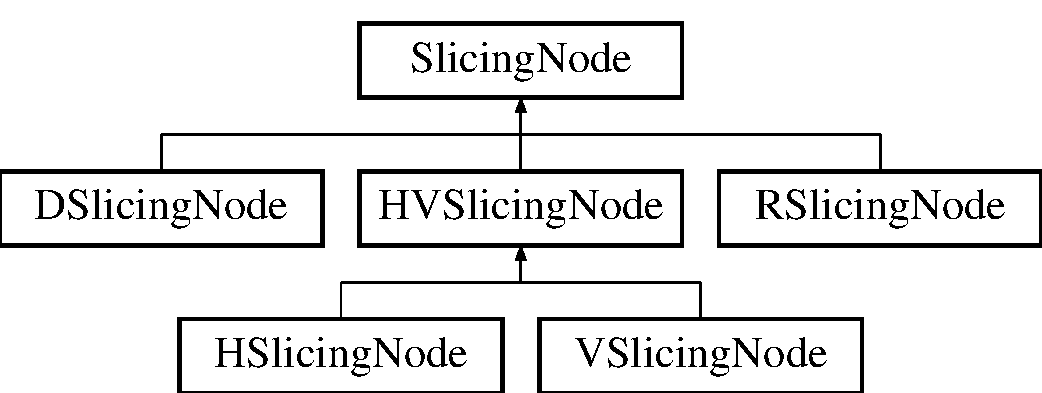
\includegraphics[height=3.000000cm]{class_open_chams_1_1_slicing_node}
\end{center}
\end{figure}

\hypertarget{class_s_p_i_c_e_1_1_source}{}\section{Source Class Reference}
\label{class_s_p_i_c_e_1_1_source}\index{Source@{Source}}
Inheritance diagram for Source\+:\begin{figure}[H]
\begin{center}
\leavevmode
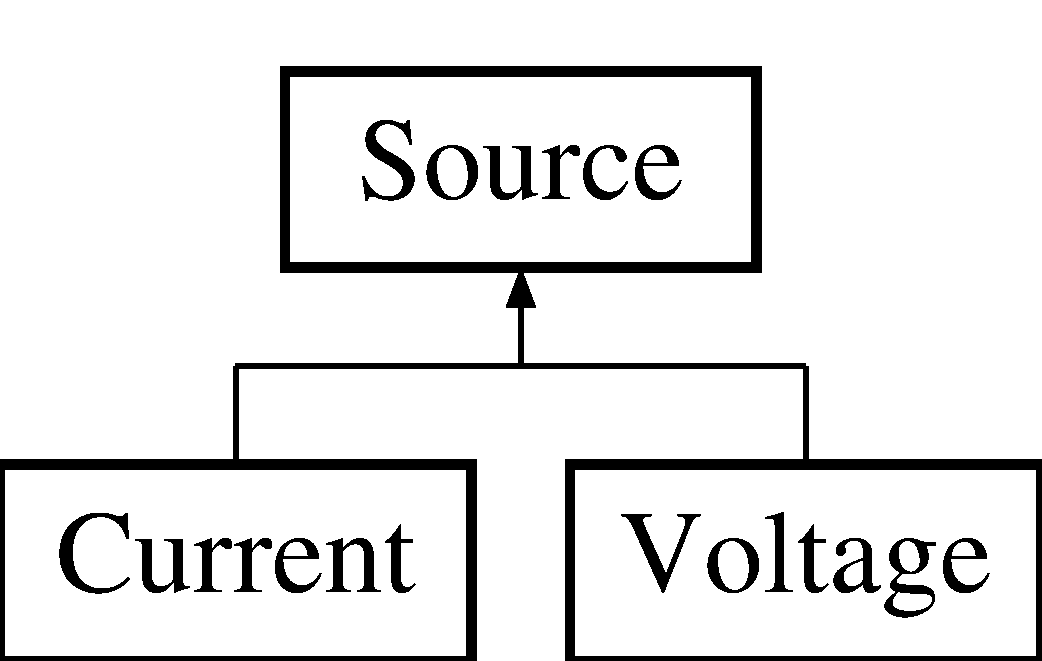
\includegraphics[height=2.000000cm]{class_s_p_i_c_e_1_1_source}
\end{center}
\end{figure}
\subsection*{Public Member Functions}
\begin{DoxyCompactItemize}
\item 
\mbox{\Hypertarget{class_s_p_i_c_e_1_1_source_ac0fc966d4386ddb71d99361e3fccb311}\label{class_s_p_i_c_e_1_1_source_ac0fc966d4386ddb71d99361e3fccb311}} 
std\+::string \hyperlink{class_s_p_i_c_e_1_1_source_ac0fc966d4386ddb71d99361e3fccb311}{get\+Name} ()
\begin{DoxyCompactList}\small\item\em returns the name of the source. \end{DoxyCompactList}\item 
\mbox{\Hypertarget{class_s_p_i_c_e_1_1_source_a8b4ab73ed1d99c533aa22af0a37ebb0d}\label{class_s_p_i_c_e_1_1_source_a8b4ab73ed1d99c533aa22af0a37ebb0d}} 
std\+::string \hyperlink{class_s_p_i_c_e_1_1_source_a8b4ab73ed1d99c533aa22af0a37ebb0d}{get\+Negative} ()
\begin{DoxyCompactList}\small\item\em returns the negative connector of the source. \end{DoxyCompactList}\item 
\mbox{\Hypertarget{class_s_p_i_c_e_1_1_source_a1adb347b9a2c2da556e4417ab0eec0e1}\label{class_s_p_i_c_e_1_1_source_a1adb347b9a2c2da556e4417ab0eec0e1}} 
std\+::string \hyperlink{class_s_p_i_c_e_1_1_source_a1adb347b9a2c2da556e4417ab0eec0e1}{get\+Positive} ()
\begin{DoxyCompactList}\small\item\em returns the positive connector of the source. \end{DoxyCompactList}\item 
\mbox{\Hypertarget{class_s_p_i_c_e_1_1_source_a4c052cb2622c580a250b2c783a436882}\label{class_s_p_i_c_e_1_1_source_a4c052cb2622c580a250b2c783a436882}} 
std\+::string \hyperlink{class_s_p_i_c_e_1_1_source_a4c052cb2622c580a250b2c783a436882}{get\+Value} ()
\begin{DoxyCompactList}\small\item\em returns the value of the source. \end{DoxyCompactList}\end{DoxyCompactItemize}
\subsection*{Protected Member Functions}
\begin{DoxyCompactItemize}
\item 
\hyperlink{class_s_p_i_c_e_1_1_source_a35145400f091a09eed7baa19128a3bc8}{Source} (std\+::string name, std\+::string pos, std\+::string neg, std\+::string value)
\begin{DoxyCompactList}\small\item\em creates a new source. \end{DoxyCompactList}\end{DoxyCompactItemize}


\subsection{Detailed Description}
This abstract class is a base class for \hyperlink{class_s_p_i_c_e_1_1_current}{S\+P\+I\+C\+E\+::\+Current} and \hyperlink{class_s_p_i_c_e_1_1_voltage}{S\+P\+I\+C\+E\+::\+Voltage} sources. 

\subsection{Constructor \& Destructor Documentation}
\mbox{\Hypertarget{class_s_p_i_c_e_1_1_source_a35145400f091a09eed7baa19128a3bc8}\label{class_s_p_i_c_e_1_1_source_a35145400f091a09eed7baa19128a3bc8}} 
\index{S\+P\+I\+C\+E\+::\+Source@{S\+P\+I\+C\+E\+::\+Source}!Source@{Source}}
\index{Source@{Source}!S\+P\+I\+C\+E\+::\+Source@{S\+P\+I\+C\+E\+::\+Source}}
\subsubsection{\texorpdfstring{Source()}{Source()}}
{\footnotesize\ttfamily \hyperlink{class_s_p_i_c_e_1_1_source}{Source} (\begin{DoxyParamCaption}\item[{std\+::string}]{name,  }\item[{std\+::string}]{pos,  }\item[{std\+::string}]{neg,  }\item[{std\+::string}]{value }\end{DoxyParamCaption})\hspace{0.3cm}{\ttfamily [inline]}, {\ttfamily [protected]}}



creates a new source. 


\begin{DoxyParams}{Parameters}
{\em name} & the name of the source. \\
\hline
{\em pos} & the positive connector of the source. \\
\hline
{\em neg} & the negative connector of the source. \\
\hline
{\em value} & the value of the source. \\
\hline
\end{DoxyParams}

\hypertarget{class_s_p_i_c_e_1_1_spice_exception}{\section{Spice\-Exception Class Reference}
\label{class_s_p_i_c_e_1_1_spice_exception}\index{Spice\-Exception@{Spice\-Exception}}
}


\subsection{Detailed Description}
This class describes the exceptions throwed by the Spice library in case of errors. 
\hypertarget{class_a_g_d_s_1_1_structure}{}\section{Structure Class Reference}
\label{class_a_g_d_s_1_1_structure}\index{Structure@{Structure}}
\subsection*{Public Member Functions}
\begin{DoxyCompactItemize}
\item 
bool \hyperlink{class_a_g_d_s_1_1_structure_a2dd203e6770f7d15d6f706867c919a60}{add\+Element} (\hyperlink{class_a_g_d_s_1_1_element}{Element} $\ast$)
\begin{DoxyCompactList}\small\item\em adds an \hyperlink{class_a_g_d_s_1_1_element}{Element} to the \hyperlink{class_a_g_d_s_1_1_structure}{Structure}. \end{DoxyCompactList}\item 
\mbox{\Hypertarget{class_a_g_d_s_1_1_structure_ac0fc966d4386ddb71d99361e3fccb311}\label{class_a_g_d_s_1_1_structure_ac0fc966d4386ddb71d99361e3fccb311}} 
std\+::string \hyperlink{class_a_g_d_s_1_1_structure_ac0fc966d4386ddb71d99361e3fccb311}{get\+Name} ()
\begin{DoxyCompactList}\small\item\em returns the name of the \hyperlink{class_a_g_d_s_1_1_structure}{Structure}. \end{DoxyCompactList}\item 
\hyperlink{class_a_g_d_s_1_1_structure_a797bfd2e6684bb9870c8070b4ef6ff41}{Structure} (std\+::string str\+Name)
\begin{DoxyCompactList}\small\item\em creates a new \hyperlink{class_a_g_d_s_1_1_structure}{Structure} \end{DoxyCompactList}\end{DoxyCompactItemize}


\subsection{Detailed Description}
This class describes a G\+DS \hyperlink{class_a_g_d_s_1_1_structure}{Structure} with a name and a list of Elements. 

\subsection{Constructor \& Destructor Documentation}
\mbox{\Hypertarget{class_a_g_d_s_1_1_structure_a797bfd2e6684bb9870c8070b4ef6ff41}\label{class_a_g_d_s_1_1_structure_a797bfd2e6684bb9870c8070b4ef6ff41}} 
\index{A\+G\+D\+S\+::\+Structure@{A\+G\+D\+S\+::\+Structure}!Structure@{Structure}}
\index{Structure@{Structure}!A\+G\+D\+S\+::\+Structure@{A\+G\+D\+S\+::\+Structure}}
\subsubsection{\texorpdfstring{Structure()}{Structure()}}
{\footnotesize\ttfamily \hyperlink{class_a_g_d_s_1_1_structure}{Structure} (\begin{DoxyParamCaption}\item[{std\+::string}]{name }\end{DoxyParamCaption})}



creates a new \hyperlink{class_a_g_d_s_1_1_structure}{Structure} 


\begin{DoxyParams}{Parameters}
{\em name} & the name of the structure. \\
\hline
\end{DoxyParams}


\subsection{Member Function Documentation}
\mbox{\Hypertarget{class_a_g_d_s_1_1_structure_a2dd203e6770f7d15d6f706867c919a60}\label{class_a_g_d_s_1_1_structure_a2dd203e6770f7d15d6f706867c919a60}} 
\index{A\+G\+D\+S\+::\+Structure@{A\+G\+D\+S\+::\+Structure}!add\+Element@{add\+Element}}
\index{add\+Element@{add\+Element}!A\+G\+D\+S\+::\+Structure@{A\+G\+D\+S\+::\+Structure}}
\subsubsection{\texorpdfstring{add\+Element()}{addElement()}}
{\footnotesize\ttfamily bool add\+Element (\begin{DoxyParamCaption}\item[{\hyperlink{class_a_g_d_s_1_1_element}{Element} $\ast$}]{element }\end{DoxyParamCaption})}



adds an \hyperlink{class_a_g_d_s_1_1_element}{Element} to the \hyperlink{class_a_g_d_s_1_1_structure}{Structure}. 


\begin{DoxyParams}{Parameters}
{\em element} & the \hyperlink{class_a_g_d_s_1_1_element}{Element} object to add. \\
\hline
\end{DoxyParams}

\hypertarget{class_s_p_i_c_e_1_1_subckt}{}\section{Subckt Class Reference}
\label{class_s_p_i_c_e_1_1_subckt}\index{Subckt@{Subckt}}
\subsection*{Public Member Functions}
\begin{DoxyCompactItemize}
\item 
void \hyperlink{class_s_p_i_c_e_1_1_subckt_a6c590c1d92248d6e5f95ea6c470fbb5a}{add\+Comment} (std\+::string)
\begin{DoxyCompactList}\small\item\em adds a comment to the subckt. \end{DoxyCompactList}\item 
void \hyperlink{class_s_p_i_c_e_1_1_subckt_a7bb4a4532643568ab1ac2c229185a88e}{add\+Instance} (\hyperlink{class_s_p_i_c_e_1_1_instance}{Instance} $\ast$)
\begin{DoxyCompactList}\small\item\em adds an instance to the subckt. \end{DoxyCompactList}\item 
void \hyperlink{class_s_p_i_c_e_1_1_subckt_ac162264683fa3d9b3384d3e8cc291fa2}{add\+Interface} (std\+::string)
\begin{DoxyCompactList}\small\item\em adds an interface to the subckt. \end{DoxyCompactList}\item 
void \hyperlink{class_s_p_i_c_e_1_1_subckt_ab3ab147a16bc490ce96db905a4ca271c}{add\+Parameter} (std\+::string, std\+::string)
\begin{DoxyCompactList}\small\item\em adds a parameter to the subckt. \end{DoxyCompactList}\item 
const std\+::vector$<$ std\+::string $>$ \& \hyperlink{class_s_p_i_c_e_1_1_subckt_aa4a73ef909ceb8d442ed2f205967613a}{get\+Comments} ()
\begin{DoxyCompactList}\small\item\em returns the comments of the subckt. \end{DoxyCompactList}\item 
\mbox{\Hypertarget{class_s_p_i_c_e_1_1_subckt_a8e6e58ffab876152a740092520c35d73}\label{class_s_p_i_c_e_1_1_subckt_a8e6e58ffab876152a740092520c35d73}} 
const std\+::vector$<$ \hyperlink{class_s_p_i_c_e_1_1_instance}{Instance} $\ast$ $>$ \& \hyperlink{class_s_p_i_c_e_1_1_subckt_a8e6e58ffab876152a740092520c35d73}{get\+Instances} ()
\begin{DoxyCompactList}\small\item\em returns the instances of the subckt. \end{DoxyCompactList}\item 
\mbox{\Hypertarget{class_s_p_i_c_e_1_1_subckt_a5df00fe6eb5e287abef28c76ce88bd1e}\label{class_s_p_i_c_e_1_1_subckt_a5df00fe6eb5e287abef28c76ce88bd1e}} 
const std\+::vector$<$ std\+::string $>$ \& \hyperlink{class_s_p_i_c_e_1_1_subckt_a5df00fe6eb5e287abef28c76ce88bd1e}{get\+Interfaces} ()
\begin{DoxyCompactList}\small\item\em returns the interfaces of the subckt. \end{DoxyCompactList}\item 
\mbox{\Hypertarget{class_s_p_i_c_e_1_1_subckt_af55b1fe10eacd22c7ff3544b5ed32ef3}\label{class_s_p_i_c_e_1_1_subckt_af55b1fe10eacd22c7ff3544b5ed32ef3}} 
const std\+::string \hyperlink{class_s_p_i_c_e_1_1_subckt_af55b1fe10eacd22c7ff3544b5ed32ef3}{get\+Name} ()
\begin{DoxyCompactList}\small\item\em returns the name of the subckt. \end{DoxyCompactList}\item 
\mbox{\Hypertarget{class_s_p_i_c_e_1_1_subckt_aee7d59083b78d31ac5c19ab508da91e0}\label{class_s_p_i_c_e_1_1_subckt_aee7d59083b78d31ac5c19ab508da91e0}} 
const std\+::map$<$ std\+::string, std\+::string $>$ \& \hyperlink{class_s_p_i_c_e_1_1_subckt_aee7d59083b78d31ac5c19ab508da91e0}{get\+Parameters} ()
\begin{DoxyCompactList}\small\item\em returns the parameters of the subckt. \end{DoxyCompactList}\item 
\hyperlink{class_s_p_i_c_e_1_1_subckt_a5b9ee31a0302af435029f29a93b29d7d}{Subckt} (std\+::string name)
\begin{DoxyCompactList}\small\item\em creates a new subckt. \end{DoxyCompactList}\end{DoxyCompactItemize}


\subsection{Detailed Description}
This class describes a subckt of the global circuit. 

\subsection{Constructor \& Destructor Documentation}
\mbox{\Hypertarget{class_s_p_i_c_e_1_1_subckt_a5b9ee31a0302af435029f29a93b29d7d}\label{class_s_p_i_c_e_1_1_subckt_a5b9ee31a0302af435029f29a93b29d7d}} 
\index{S\+P\+I\+C\+E\+::\+Subckt@{S\+P\+I\+C\+E\+::\+Subckt}!Subckt@{Subckt}}
\index{Subckt@{Subckt}!S\+P\+I\+C\+E\+::\+Subckt@{S\+P\+I\+C\+E\+::\+Subckt}}
\subsubsection{\texorpdfstring{Subckt()}{Subckt()}}
{\footnotesize\ttfamily \hyperlink{class_s_p_i_c_e_1_1_subckt}{Subckt} (\begin{DoxyParamCaption}\item[{std\+::string}]{name }\end{DoxyParamCaption})\hspace{0.3cm}{\ttfamily [inline]}}



creates a new subckt. 


\begin{DoxyParams}{Parameters}
{\em name} & the name of the subckt \\
\hline
\end{DoxyParams}


\subsection{Member Function Documentation}
\mbox{\Hypertarget{class_s_p_i_c_e_1_1_subckt_a6c590c1d92248d6e5f95ea6c470fbb5a}\label{class_s_p_i_c_e_1_1_subckt_a6c590c1d92248d6e5f95ea6c470fbb5a}} 
\index{S\+P\+I\+C\+E\+::\+Subckt@{S\+P\+I\+C\+E\+::\+Subckt}!add\+Comment@{add\+Comment}}
\index{add\+Comment@{add\+Comment}!S\+P\+I\+C\+E\+::\+Subckt@{S\+P\+I\+C\+E\+::\+Subckt}}
\subsubsection{\texorpdfstring{add\+Comment()}{addComment()}}
{\footnotesize\ttfamily void add\+Comment (\begin{DoxyParamCaption}\item[{std\+::string}]{comment }\end{DoxyParamCaption})\hspace{0.3cm}{\ttfamily [inline]}}



adds a comment to the subckt. 


\begin{DoxyParams}{Parameters}
{\em comment} & the comment to add.\\
\hline
\end{DoxyParams}
\begin{DoxyNote}{Note}
comments of a subckt are the first lines of the subckt to describe the interfaces of the subckt. 
\end{DoxyNote}
\mbox{\Hypertarget{class_s_p_i_c_e_1_1_subckt_a7bb4a4532643568ab1ac2c229185a88e}\label{class_s_p_i_c_e_1_1_subckt_a7bb4a4532643568ab1ac2c229185a88e}} 
\index{S\+P\+I\+C\+E\+::\+Subckt@{S\+P\+I\+C\+E\+::\+Subckt}!add\+Instance@{add\+Instance}}
\index{add\+Instance@{add\+Instance}!S\+P\+I\+C\+E\+::\+Subckt@{S\+P\+I\+C\+E\+::\+Subckt}}
\subsubsection{\texorpdfstring{add\+Instance()}{addInstance()}}
{\footnotesize\ttfamily void add\+Instance (\begin{DoxyParamCaption}\item[{\hyperlink{class_s_p_i_c_e_1_1_instance}{Instance} $\ast$}]{instance }\end{DoxyParamCaption})\hspace{0.3cm}{\ttfamily [inline]}}



adds an instance to the subckt. 


\begin{DoxyParams}{Parameters}
{\em instance} & the instance to add. \\
\hline
\end{DoxyParams}
\mbox{\Hypertarget{class_s_p_i_c_e_1_1_subckt_ac162264683fa3d9b3384d3e8cc291fa2}\label{class_s_p_i_c_e_1_1_subckt_ac162264683fa3d9b3384d3e8cc291fa2}} 
\index{S\+P\+I\+C\+E\+::\+Subckt@{S\+P\+I\+C\+E\+::\+Subckt}!add\+Interface@{add\+Interface}}
\index{add\+Interface@{add\+Interface}!S\+P\+I\+C\+E\+::\+Subckt@{S\+P\+I\+C\+E\+::\+Subckt}}
\subsubsection{\texorpdfstring{add\+Interface()}{addInterface()}}
{\footnotesize\ttfamily void add\+Interface (\begin{DoxyParamCaption}\item[{std\+::string}]{name }\end{DoxyParamCaption})\hspace{0.3cm}{\ttfamily [inline]}}



adds an interface to the subckt. 


\begin{DoxyParams}{Parameters}
{\em name} & the name of the interface to add. \\
\hline
\end{DoxyParams}
\mbox{\Hypertarget{class_s_p_i_c_e_1_1_subckt_ab3ab147a16bc490ce96db905a4ca271c}\label{class_s_p_i_c_e_1_1_subckt_ab3ab147a16bc490ce96db905a4ca271c}} 
\index{S\+P\+I\+C\+E\+::\+Subckt@{S\+P\+I\+C\+E\+::\+Subckt}!add\+Parameter@{add\+Parameter}}
\index{add\+Parameter@{add\+Parameter}!S\+P\+I\+C\+E\+::\+Subckt@{S\+P\+I\+C\+E\+::\+Subckt}}
\subsubsection{\texorpdfstring{add\+Parameter()}{addParameter()}}
{\footnotesize\ttfamily void add\+Parameter (\begin{DoxyParamCaption}\item[{std\+::string}]{name,  }\item[{std\+::string}]{value }\end{DoxyParamCaption})}



adds a parameter to the subckt. 


\begin{DoxyParams}{Parameters}
{\em name} & the name of the parameter to add. \\
\hline
{\em value} & the value of the parameter to add. \\
\hline
\end{DoxyParams}
\mbox{\Hypertarget{class_s_p_i_c_e_1_1_subckt_aa4a73ef909ceb8d442ed2f205967613a}\label{class_s_p_i_c_e_1_1_subckt_aa4a73ef909ceb8d442ed2f205967613a}} 
\index{S\+P\+I\+C\+E\+::\+Subckt@{S\+P\+I\+C\+E\+::\+Subckt}!get\+Comments@{get\+Comments}}
\index{get\+Comments@{get\+Comments}!S\+P\+I\+C\+E\+::\+Subckt@{S\+P\+I\+C\+E\+::\+Subckt}}
\subsubsection{\texorpdfstring{get\+Comments()}{getComments()}}
{\footnotesize\ttfamily const std\+::vector$<$ std\+::string $>$ \& get\+Comments (\begin{DoxyParamCaption}{ }\end{DoxyParamCaption})\hspace{0.3cm}{\ttfamily [inline]}}



returns the comments of the subckt. 

\begin{DoxyNote}{Note}
comments of a subckt are the first lines of the subckt to describe the interfaces of the subckt. 
\end{DoxyNote}

\hypertarget{class_d_t_r_1_1_techno}{}\section{Techno Class Reference}
\label{class_d_t_r_1_1_techno}\index{Techno@{Techno}}
\subsection*{Public Member Functions}
\begin{DoxyCompactItemize}
\item 
\hyperlink{class_d_t_r_1_1_a_rule}{A\+Rule} $\ast$ \hyperlink{class_d_t_r_1_1_techno_a5f5a790974fe7d3b1c6f1b698ef0a818}{add\+A\+Rule} (const char $\ast$name, double value, const char $\ast$ref, const char $\ast$layer1, const char $\ast$layer2)
\begin{DoxyCompactList}\small\item\em creates a new \hyperlink{class_d_t_r_1_1_a_rule}{A\+Rule} and adds it to the \hyperlink{class_d_t_r_1_1_techno}{Techno} object. \end{DoxyCompactList}\item 
\hyperlink{class_d_t_r_1_1_rule}{Rule} $\ast$ \hyperlink{class_d_t_r_1_1_techno_afa2c8412c365c950649b9f81661ecafd}{add\+Rule} (const char $\ast$name, double value, const char $\ast$ref, const char $\ast$layer1=\char`\"{}\char`\"{}, const char $\ast$layer2=\char`\"{}\char`\"{})
\begin{DoxyCompactList}\small\item\em creates a new \hyperlink{class_d_t_r_1_1_rule}{Rule} and adds it the to \hyperlink{class_d_t_r_1_1_techno}{Techno} object. \end{DoxyCompactList}\item 
\mbox{\Hypertarget{class_d_t_r_1_1_techno_a3fd7335faa33dce2f87c7e50eef3e294}\label{class_d_t_r_1_1_techno_a3fd7335faa33dce2f87c7e50eef3e294}} 
const std\+::string \& \hyperlink{class_d_t_r_1_1_techno_a3fd7335faa33dce2f87c7e50eef3e294}{get\+Name} () const
\begin{DoxyCompactList}\small\item\em returns the name of the technology. \end{DoxyCompactList}\item 
\hyperlink{class_d_t_r_1_1_rule}{Rule} $\ast$ \hyperlink{class_d_t_r_1_1_techno_a4d56a05b47bd6c51e4e18120f49b584b}{get\+Rule} (const char $\ast$name, const char $\ast$layer1=\char`\"{}\char`\"{}, const char $\ast$layer2=\char`\"{}\char`\"{})
\begin{DoxyCompactList}\small\item\em returns the rule uniquely identified by its name and layers. \end{DoxyCompactList}\item 
std\+::vector$<$ \hyperlink{class_d_t_r_1_1_rule}{Rule} $\ast$ $>$ \& \hyperlink{class_d_t_r_1_1_techno_ac322d0479195cd8a65ff5a922b7f2af7}{get\+Rules} ()
\begin{DoxyCompactList}\small\item\em returns a reference on the std\+::vector containing all technology\textquotesingle{}s rules. \end{DoxyCompactList}\item 
\mbox{\Hypertarget{class_d_t_r_1_1_techno_a42e12e8f890c03ebf12e754d7e489dcb}\label{class_d_t_r_1_1_techno_a42e12e8f890c03ebf12e754d7e489dcb}} 
const std\+::string \& \hyperlink{class_d_t_r_1_1_techno_a42e12e8f890c03ebf12e754d7e489dcb}{get\+Unit} () const
\begin{DoxyCompactList}\small\item\em returns the unit. \end{DoxyCompactList}\item 
double \hyperlink{class_d_t_r_1_1_techno_ac08e2e60dd16750551221ca908001057}{get\+Value} (const char $\ast$name, const char $\ast$layer1=\char`\"{}\char`\"{}, const char $\ast$layer2=\char`\"{}\char`\"{})
\begin{DoxyCompactList}\small\item\em returns the value of a rule uniquely identified by its name and layers. \end{DoxyCompactList}\item 
const std\+::string \& \hyperlink{class_d_t_r_1_1_techno_ad5ef5b8e444ab7a86a2e3bff7762c956}{get\+Value\+As\+String} (const char $\ast$name, const char $\ast$layer1=\char`\"{}\char`\"{}, const char $\ast$layer2=\char`\"{}\char`\"{})
\begin{DoxyCompactList}\small\item\em returns a string corresponding to the value of a rule uniquely identified by its name and layers. \end{DoxyCompactList}\item 
\hyperlink{class_d_t_r_1_1_techno_a25c6aecdd011d09618908626192c933f}{Techno} (const char $\ast$name, const char $\ast$unit, const char $\ast$version)
\begin{DoxyCompactList}\small\item\em creates a new technology \end{DoxyCompactList}\item 
bool \hyperlink{class_d_t_r_1_1_techno_a26b05539dd3345963b8708788b82e2cb}{write\+To\+File} (const char $\ast$file\+Path)
\begin{DoxyCompactList}\small\item\em writes the database to file. \end{DoxyCompactList}\end{DoxyCompactItemize}
\subsection*{Static Public Member Functions}
\begin{DoxyCompactItemize}
\item 
static \hyperlink{class_d_t_r_1_1_techno}{Techno} $\ast$ \hyperlink{class_d_t_r_1_1_techno_acf863c2bdb7f1aacc4422c8155c60d17}{read\+From\+File} (const char $\ast$file\+Path)
\begin{DoxyCompactList}\small\item\em creates and returns a \hyperlink{class_d_t_r_1_1_techno}{Techno} object based on a database source file. \end{DoxyCompactList}\end{DoxyCompactItemize}


\subsection{Detailed Description}
This class contains generic informations such as the name of the technology and the unit used, and the list of all technologic rules. 

\subsection{Constructor \& Destructor Documentation}
\mbox{\Hypertarget{class_d_t_r_1_1_techno_a25c6aecdd011d09618908626192c933f}\label{class_d_t_r_1_1_techno_a25c6aecdd011d09618908626192c933f}} 
\index{D\+T\+R\+::\+Techno@{D\+T\+R\+::\+Techno}!Techno@{Techno}}
\index{Techno@{Techno}!D\+T\+R\+::\+Techno@{D\+T\+R\+::\+Techno}}
\subsubsection{\texorpdfstring{Techno()}{Techno()}}
{\footnotesize\ttfamily \hyperlink{class_d_t_r_1_1_techno}{Techno} (\begin{DoxyParamCaption}\item[{const char $\ast$}]{name,  }\item[{const char $\ast$}]{unit,  }\item[{const char $\ast$}]{version }\end{DoxyParamCaption})}



creates a new technology 


\begin{DoxyParams}{Parameters}
{\em name} & the name of the technology. \\
\hline
{\em unit} & the unit used for all values. \\
\hline
{\em version} & the technology version/revision. \\
\hline
\end{DoxyParams}


\subsection{Member Function Documentation}
\mbox{\Hypertarget{class_d_t_r_1_1_techno_a5f5a790974fe7d3b1c6f1b698ef0a818}\label{class_d_t_r_1_1_techno_a5f5a790974fe7d3b1c6f1b698ef0a818}} 
\index{D\+T\+R\+::\+Techno@{D\+T\+R\+::\+Techno}!add\+A\+Rule@{add\+A\+Rule}}
\index{add\+A\+Rule@{add\+A\+Rule}!D\+T\+R\+::\+Techno@{D\+T\+R\+::\+Techno}}
\subsubsection{\texorpdfstring{add\+A\+Rule()}{addARule()}}
{\footnotesize\ttfamily \hyperlink{class_d_t_r_1_1_a_rule}{A\+Rule} $\ast$ add\+A\+Rule (\begin{DoxyParamCaption}\item[{const char $\ast$}]{name,  }\item[{double}]{value,  }\item[{const char $\ast$}]{ref,  }\item[{const char $\ast$}]{layer1,  }\item[{const char $\ast$}]{layer2 }\end{DoxyParamCaption})}



creates a new \hyperlink{class_d_t_r_1_1_a_rule}{A\+Rule} and adds it to the \hyperlink{class_d_t_r_1_1_techno}{Techno} object. 


\begin{DoxyParams}{Parameters}
{\em name} & the name of the rule. \\
\hline
{\em value} & the value of the rule. \\
\hline
{\em ref} & the reference of the rule (helpful to find the rule in design kit). \\
\hline
{\em layer1} & the first layer. \\
\hline
{\em layer2} & the second layer.\\
\hline
\end{DoxyParams}
\begin{DoxyReturn}{Returns}
the newly created \hyperlink{class_d_t_r_1_1_a_rule}{A\+Rule} object. 
\end{DoxyReturn}
\mbox{\Hypertarget{class_d_t_r_1_1_techno_afa2c8412c365c950649b9f81661ecafd}\label{class_d_t_r_1_1_techno_afa2c8412c365c950649b9f81661ecafd}} 
\index{D\+T\+R\+::\+Techno@{D\+T\+R\+::\+Techno}!add\+Rule@{add\+Rule}}
\index{add\+Rule@{add\+Rule}!D\+T\+R\+::\+Techno@{D\+T\+R\+::\+Techno}}
\subsubsection{\texorpdfstring{add\+Rule()}{addRule()}}
{\footnotesize\ttfamily \hyperlink{class_d_t_r_1_1_rule}{Rule} $\ast$ add\+Rule (\begin{DoxyParamCaption}\item[{const char $\ast$}]{name,  }\item[{double}]{value,  }\item[{const char $\ast$}]{ref,  }\item[{const char $\ast$}]{layer1 = {\ttfamily \char`\"{}\char`\"{}},  }\item[{const char $\ast$}]{layer2 = {\ttfamily \char`\"{}\char`\"{}} }\end{DoxyParamCaption})}



creates a new \hyperlink{class_d_t_r_1_1_rule}{Rule} and adds it the to \hyperlink{class_d_t_r_1_1_techno}{Techno} object. 


\begin{DoxyParams}{Parameters}
{\em name} & the name of the rule. \\
\hline
{\em value} & the value of the rule. \\
\hline
{\em ref} & the reference of the rule (helpful to find the rule in design kit). \\
\hline
{\em layer1} & the first layer. This is an optionnal argument, default value is \char`\"{}\char`\"{}. \\
\hline
{\em layer2} & the second layer. This is an optionnal argument, default value is \char`\"{}\char`\"{}.\\
\hline
\end{DoxyParams}
\begin{DoxyReturn}{Returns}
the newly created \hyperlink{class_d_t_r_1_1_rule}{Rule} object. 
\end{DoxyReturn}
\mbox{\Hypertarget{class_d_t_r_1_1_techno_a4d56a05b47bd6c51e4e18120f49b584b}\label{class_d_t_r_1_1_techno_a4d56a05b47bd6c51e4e18120f49b584b}} 
\index{D\+T\+R\+::\+Techno@{D\+T\+R\+::\+Techno}!get\+Rule@{get\+Rule}}
\index{get\+Rule@{get\+Rule}!D\+T\+R\+::\+Techno@{D\+T\+R\+::\+Techno}}
\subsubsection{\texorpdfstring{get\+Rule()}{getRule()}}
{\footnotesize\ttfamily \hyperlink{class_d_t_r_1_1_rule}{Rule} $\ast$ get\+Rule (\begin{DoxyParamCaption}\item[{const char $\ast$}]{name,  }\item[{const char $\ast$}]{layer1 = {\ttfamily \char`\"{}\char`\"{}},  }\item[{const char $\ast$}]{layer2 = {\ttfamily \char`\"{}\char`\"{}} }\end{DoxyParamCaption})}



returns the rule uniquely identified by its name and layers. 


\begin{DoxyParams}{Parameters}
{\em name} & the name of the rule. \\
\hline
{\em layer1} & the first layer. This is an optionnal argument, default value is \char`\"{}\char`\"{}. \\
\hline
{\em layer2} & the second layer. This is an optionnal argument, default value is \char`\"{}\char`\"{}.\\
\hline
\end{DoxyParams}
\begin{DoxyReturn}{Returns}
the rule. 
\end{DoxyReturn}
\mbox{\Hypertarget{class_d_t_r_1_1_techno_ac322d0479195cd8a65ff5a922b7f2af7}\label{class_d_t_r_1_1_techno_ac322d0479195cd8a65ff5a922b7f2af7}} 
\index{D\+T\+R\+::\+Techno@{D\+T\+R\+::\+Techno}!get\+Rules@{get\+Rules}}
\index{get\+Rules@{get\+Rules}!D\+T\+R\+::\+Techno@{D\+T\+R\+::\+Techno}}
\subsubsection{\texorpdfstring{get\+Rules()}{getRules()}}
{\footnotesize\ttfamily std\+::vector$<$ \hyperlink{class_d_t_r_1_1_rule}{Rule} $\ast$ $>$ \& get\+Rules (\begin{DoxyParamCaption}{ }\end{DoxyParamCaption})\hspace{0.3cm}{\ttfamily [inline]}}



returns a reference on the std\+::vector containing all technology\textquotesingle{}s rules. 

\begin{DoxyNote}{Note}
this method is not yet available in python 
\end{DoxyNote}
\mbox{\Hypertarget{class_d_t_r_1_1_techno_ac08e2e60dd16750551221ca908001057}\label{class_d_t_r_1_1_techno_ac08e2e60dd16750551221ca908001057}} 
\index{D\+T\+R\+::\+Techno@{D\+T\+R\+::\+Techno}!get\+Value@{get\+Value}}
\index{get\+Value@{get\+Value}!D\+T\+R\+::\+Techno@{D\+T\+R\+::\+Techno}}
\subsubsection{\texorpdfstring{get\+Value()}{getValue()}}
{\footnotesize\ttfamily double get\+Value (\begin{DoxyParamCaption}\item[{const char $\ast$}]{name,  }\item[{const char $\ast$}]{layer1 = {\ttfamily \char`\"{}\char`\"{}},  }\item[{const char $\ast$}]{layer2 = {\ttfamily \char`\"{}\char`\"{}} }\end{DoxyParamCaption})}



returns the value of a rule uniquely identified by its name and layers. 


\begin{DoxyParams}{Parameters}
{\em name} & the name of the rule. \\
\hline
{\em layer1} & the first layer. This is an optionnal argument, default value is \char`\"{}\char`\"{}. \\
\hline
{\em layer2} & the second layer. This is an optionnal argument, default value is \char`\"{}\char`\"{}.\\
\hline
\end{DoxyParams}
\begin{DoxyReturn}{Returns}
the value of the rule. 
\end{DoxyReturn}
\mbox{\Hypertarget{class_d_t_r_1_1_techno_ad5ef5b8e444ab7a86a2e3bff7762c956}\label{class_d_t_r_1_1_techno_ad5ef5b8e444ab7a86a2e3bff7762c956}} 
\index{D\+T\+R\+::\+Techno@{D\+T\+R\+::\+Techno}!get\+Value\+As\+String@{get\+Value\+As\+String}}
\index{get\+Value\+As\+String@{get\+Value\+As\+String}!D\+T\+R\+::\+Techno@{D\+T\+R\+::\+Techno}}
\subsubsection{\texorpdfstring{get\+Value\+As\+String()}{getValueAsString()}}
{\footnotesize\ttfamily const string \& get\+Value\+As\+String (\begin{DoxyParamCaption}\item[{const char $\ast$}]{name,  }\item[{const char $\ast$}]{layer1 = {\ttfamily \char`\"{}\char`\"{}},  }\item[{const char $\ast$}]{layer2 = {\ttfamily \char`\"{}\char`\"{}} }\end{DoxyParamCaption})}



returns a string corresponding to the value of a rule uniquely identified by its name and layers. 


\begin{DoxyParams}{Parameters}
{\em name} & the name of the rule. \\
\hline
{\em layer1} & the first layer. This is an optionnal argument, default value is \char`\"{}\char`\"{}. \\
\hline
{\em layer2} & the second layer. This is an optionnal argument, default value is \char`\"{}\char`\"{}.\\
\hline
\end{DoxyParams}
\begin{DoxyReturn}{Returns}
the string corresponding to the value of the rule.
\end{DoxyReturn}
\begin{DoxyNote}{Note}
this method is important for python module since to avoid rounding problems it is necessary to use Decimal object which is build based on a string. 
\end{DoxyNote}
\mbox{\Hypertarget{class_d_t_r_1_1_techno_acf863c2bdb7f1aacc4422c8155c60d17}\label{class_d_t_r_1_1_techno_acf863c2bdb7f1aacc4422c8155c60d17}} 
\index{D\+T\+R\+::\+Techno@{D\+T\+R\+::\+Techno}!read\+From\+File@{read\+From\+File}}
\index{read\+From\+File@{read\+From\+File}!D\+T\+R\+::\+Techno@{D\+T\+R\+::\+Techno}}
\subsubsection{\texorpdfstring{read\+From\+File()}{readFromFile()}}
{\footnotesize\ttfamily \hyperlink{class_d_t_r_1_1_techno}{Techno} $\ast$ read\+From\+File (\begin{DoxyParamCaption}\item[{const char $\ast$}]{filename }\end{DoxyParamCaption})\hspace{0.3cm}{\ttfamily [static]}}



creates and returns a \hyperlink{class_d_t_r_1_1_techno}{Techno} object based on a database source file. 


\begin{DoxyParams}{Parameters}
{\em filename} & the source file name.\\
\hline
\end{DoxyParams}
\begin{DoxyReturn}{Returns}
the newly created \hyperlink{class_d_t_r_1_1_techno}{Techno}. 
\end{DoxyReturn}
\mbox{\Hypertarget{class_d_t_r_1_1_techno_a26b05539dd3345963b8708788b82e2cb}\label{class_d_t_r_1_1_techno_a26b05539dd3345963b8708788b82e2cb}} 
\index{D\+T\+R\+::\+Techno@{D\+T\+R\+::\+Techno}!write\+To\+File@{write\+To\+File}}
\index{write\+To\+File@{write\+To\+File}!D\+T\+R\+::\+Techno@{D\+T\+R\+::\+Techno}}
\subsubsection{\texorpdfstring{write\+To\+File()}{writeToFile()}}
{\footnotesize\ttfamily bool write\+To\+File (\begin{DoxyParamCaption}\item[{const char $\ast$}]{filename }\end{DoxyParamCaption})}



writes the database to file. 


\begin{DoxyParams}{Parameters}
{\em filename} & the destination file name. \\
\hline
\end{DoxyParams}

\hypertarget{class_open_chams_1_1_transistor}{\section{Transistor Class Reference}
\label{class_open_chams_1_1_transistor}\index{Transistor@{Transistor}}
}
\subsection*{Public Member Functions}
\begin{DoxyCompactItemize}
\item 
\hypertarget{class_open_chams_1_1_transistor_a27ba43f825f9243556ec65d306a2b1a7}{const std\-::string \& \hyperlink{class_open_chams_1_1_transistor_a27ba43f825f9243556ec65d306a2b1a7}{get\-Bulk} ()}\label{class_open_chams_1_1_transistor_a27ba43f825f9243556ec65d306a2b1a7}

\begin{DoxyCompactList}\small\item\em returns the name of the net connected to the transistor's bulk. \end{DoxyCompactList}\item 
\hypertarget{class_open_chams_1_1_transistor_a62ea0998b3a61310a8331873f5bcce58}{const std\-::string \& \hyperlink{class_open_chams_1_1_transistor_a62ea0998b3a61310a8331873f5bcce58}{get\-Drain} ()}\label{class_open_chams_1_1_transistor_a62ea0998b3a61310a8331873f5bcce58}

\begin{DoxyCompactList}\small\item\em returns the name of the net connected to the transistor's drain. \end{DoxyCompactList}\item 
\hypertarget{class_open_chams_1_1_transistor_a99f1449aa735ff6cb4927b4f6aa34d9d}{const std\-::string \& \hyperlink{class_open_chams_1_1_transistor_a99f1449aa735ff6cb4927b4f6aa34d9d}{get\-Gate} ()}\label{class_open_chams_1_1_transistor_a99f1449aa735ff6cb4927b4f6aa34d9d}

\begin{DoxyCompactList}\small\item\em returns the name of the net connected to the transistor's gate. \end{DoxyCompactList}\item 
\hypertarget{class_open_chams_1_1_transistor_a2858c0c4e8b5108f041237cf5a802029}{const std\-::string \& \hyperlink{class_open_chams_1_1_transistor_a2858c0c4e8b5108f041237cf5a802029}{get\-Name} ()}\label{class_open_chams_1_1_transistor_a2858c0c4e8b5108f041237cf5a802029}

\begin{DoxyCompactList}\small\item\em returns the name of the transistor. \end{DoxyCompactList}\item 
\hypertarget{class_open_chams_1_1_transistor_a2e51ad4344607fc279c5c8cda4edae02}{\hyperlink{class_open_chams_1_1_parameters}{Parameters} \hyperlink{class_open_chams_1_1_transistor_a2e51ad4344607fc279c5c8cda4edae02}{get\-Parameters} ()}\label{class_open_chams_1_1_transistor_a2e51ad4344607fc279c5c8cda4edae02}

\begin{DoxyCompactList}\small\item\em returns the parameters of the instance. \end{DoxyCompactList}\item 
\hypertarget{class_open_chams_1_1_transistor_aee4d52a0b13e6db247c1a6c051aede25}{const std\-::string \& \hyperlink{class_open_chams_1_1_transistor_aee4d52a0b13e6db247c1a6c051aede25}{get\-Source} ()}\label{class_open_chams_1_1_transistor_aee4d52a0b13e6db247c1a6c051aede25}

\begin{DoxyCompactList}\small\item\em returns the name of the net connected to the transistor's source. \end{DoxyCompactList}\item 
void \hyperlink{class_open_chams_1_1_transistor_a1484abe63e3f8ffbc2911c5230fa7091}{set\-Bulk} (const std\-::string \&)
\begin{DoxyCompactList}\small\item\em sets the net of the transistor's bulk. \end{DoxyCompactList}\item 
void \hyperlink{class_open_chams_1_1_transistor_a72ff8491040e3fdc1c8bd62b2392ab82}{set\-Drain} (const std\-::string \&)
\begin{DoxyCompactList}\small\item\em sets the net of the transistor's drain. \end{DoxyCompactList}\item 
void \hyperlink{class_open_chams_1_1_transistor_a705b53a51f0e265533b228f6e8beaf50}{set\-Gate} (const std\-::string \&)
\begin{DoxyCompactList}\small\item\em sets the net of the transistor's gate. \end{DoxyCompactList}\item 
void \hyperlink{class_open_chams_1_1_transistor_a36c59a26f0317be12cea01f8dea24ec7}{set\-Name} (const std\-::string \&)
\begin{DoxyCompactList}\small\item\em sets the transistor's name. \end{DoxyCompactList}\item 
void \hyperlink{class_open_chams_1_1_transistor_abc4a5d86e639ea13e27551722e2f9c17}{set\-Source} (const std\-::string \&)
\begin{DoxyCompactList}\small\item\em sets the net of the transistor's source. \end{DoxyCompactList}\item 
\hyperlink{class_open_chams_1_1_transistor_a5052d5c281f8798a0b10ebfe4c0296a5}{Transistor} (const std\-::string \&, \hyperlink{class_open_chams_1_1_instance}{Instance} $\ast$)
\begin{DoxyCompactList}\small\item\em creates a new transistor. \end{DoxyCompactList}\end{DoxyCompactItemize}


\subsection{Detailed Description}
This class describes a \hyperlink{class_open_chams_1_1_transistor}{Transistor}.

The transistor object is used to describe the inside of a \hyperlink{class_open_chams_1_1_device}{Device}. The goal is to explicit the connection between the transistor and the device's nets. 

\subsection{Constructor \& Destructor Documentation}
\hypertarget{class_open_chams_1_1_transistor_a5052d5c281f8798a0b10ebfe4c0296a5}{\index{Open\-Chams\-::\-Transistor@{Open\-Chams\-::\-Transistor}!Transistor@{Transistor}}
\index{Transistor@{Transistor}!OpenChams::Transistor@{Open\-Chams\-::\-Transistor}}
\subsubsection[{Transistor}]{\setlength{\rightskip}{0pt plus 5cm}{\bf Transistor} (
\begin{DoxyParamCaption}
\item[{const std\-::string \&}]{name, }
\item[{{\bf Instance} $\ast$}]{instance}
\end{DoxyParamCaption}
)}}\label{class_open_chams_1_1_transistor_a5052d5c281f8798a0b10ebfe4c0296a5}


creates a new transistor. 


\begin{DoxyParams}{Parameters}
{\em name} & the name of the transistor. \\
\hline
{\em instance} & the instance (device) to which the transistor belongs. \\
\hline
\end{DoxyParams}


\subsection{Member Function Documentation}
\hypertarget{class_open_chams_1_1_transistor_a1484abe63e3f8ffbc2911c5230fa7091}{\index{Open\-Chams\-::\-Transistor@{Open\-Chams\-::\-Transistor}!set\-Bulk@{set\-Bulk}}
\index{set\-Bulk@{set\-Bulk}!OpenChams::Transistor@{Open\-Chams\-::\-Transistor}}
\subsubsection[{set\-Bulk}]{\setlength{\rightskip}{0pt plus 5cm}void set\-Bulk (
\begin{DoxyParamCaption}
\item[{const std\-::string \&}]{bulk}
\end{DoxyParamCaption}
)}}\label{class_open_chams_1_1_transistor_a1484abe63e3f8ffbc2911c5230fa7091}


sets the net of the transistor's bulk. 


\begin{DoxyParams}{Parameters}
{\em name} & the name of the net to connect to the bulk. \\
\hline
\end{DoxyParams}
\hypertarget{class_open_chams_1_1_transistor_a72ff8491040e3fdc1c8bd62b2392ab82}{\index{Open\-Chams\-::\-Transistor@{Open\-Chams\-::\-Transistor}!set\-Drain@{set\-Drain}}
\index{set\-Drain@{set\-Drain}!OpenChams::Transistor@{Open\-Chams\-::\-Transistor}}
\subsubsection[{set\-Drain}]{\setlength{\rightskip}{0pt plus 5cm}void set\-Drain (
\begin{DoxyParamCaption}
\item[{const std\-::string \&}]{drain}
\end{DoxyParamCaption}
)}}\label{class_open_chams_1_1_transistor_a72ff8491040e3fdc1c8bd62b2392ab82}


sets the net of the transistor's drain. 


\begin{DoxyParams}{Parameters}
{\em name} & the name of the net to connect to the drain. \\
\hline
\end{DoxyParams}
\hypertarget{class_open_chams_1_1_transistor_a705b53a51f0e265533b228f6e8beaf50}{\index{Open\-Chams\-::\-Transistor@{Open\-Chams\-::\-Transistor}!set\-Gate@{set\-Gate}}
\index{set\-Gate@{set\-Gate}!OpenChams::Transistor@{Open\-Chams\-::\-Transistor}}
\subsubsection[{set\-Gate}]{\setlength{\rightskip}{0pt plus 5cm}void set\-Gate (
\begin{DoxyParamCaption}
\item[{const std\-::string \&}]{gate}
\end{DoxyParamCaption}
)}}\label{class_open_chams_1_1_transistor_a705b53a51f0e265533b228f6e8beaf50}


sets the net of the transistor's gate. 


\begin{DoxyParams}{Parameters}
{\em name} & the name of the net to connect to the gate. \\
\hline
\end{DoxyParams}
\hypertarget{class_open_chams_1_1_transistor_a36c59a26f0317be12cea01f8dea24ec7}{\index{Open\-Chams\-::\-Transistor@{Open\-Chams\-::\-Transistor}!set\-Name@{set\-Name}}
\index{set\-Name@{set\-Name}!OpenChams::Transistor@{Open\-Chams\-::\-Transistor}}
\subsubsection[{set\-Name}]{\setlength{\rightskip}{0pt plus 5cm}void set\-Name (
\begin{DoxyParamCaption}
\item[{const std\-::string \&}]{name}
\end{DoxyParamCaption}
)\hspace{0.3cm}{\ttfamily [inline]}}}\label{class_open_chams_1_1_transistor_a36c59a26f0317be12cea01f8dea24ec7}


sets the transistor's name. 


\begin{DoxyParams}{Parameters}
{\em name} & the name of the transistor. \\
\hline
\end{DoxyParams}
\hypertarget{class_open_chams_1_1_transistor_abc4a5d86e639ea13e27551722e2f9c17}{\index{Open\-Chams\-::\-Transistor@{Open\-Chams\-::\-Transistor}!set\-Source@{set\-Source}}
\index{set\-Source@{set\-Source}!OpenChams::Transistor@{Open\-Chams\-::\-Transistor}}
\subsubsection[{set\-Source}]{\setlength{\rightskip}{0pt plus 5cm}void set\-Source (
\begin{DoxyParamCaption}
\item[{const std\-::string \&}]{source}
\end{DoxyParamCaption}
)}}\label{class_open_chams_1_1_transistor_abc4a5d86e639ea13e27551722e2f9c17}


sets the net of the transistor's source. 


\begin{DoxyParams}{Parameters}
{\em name} & the name of the net to connect to the source. \\
\hline
\end{DoxyParams}

\hypertarget{class_s_p_i_c_e_1_1_value}{\section{Value Class Reference}
\label{class_s_p_i_c_e_1_1_value}\index{Value@{Value}}
}

\hypertarget{class_s_p_i_c_e_1_1_voltage}{}\section{Voltage Class Reference}
\label{class_s_p_i_c_e_1_1_voltage}\index{Voltage@{Voltage}}
Inheritance diagram for Voltage\+:\begin{figure}[H]
\begin{center}
\leavevmode
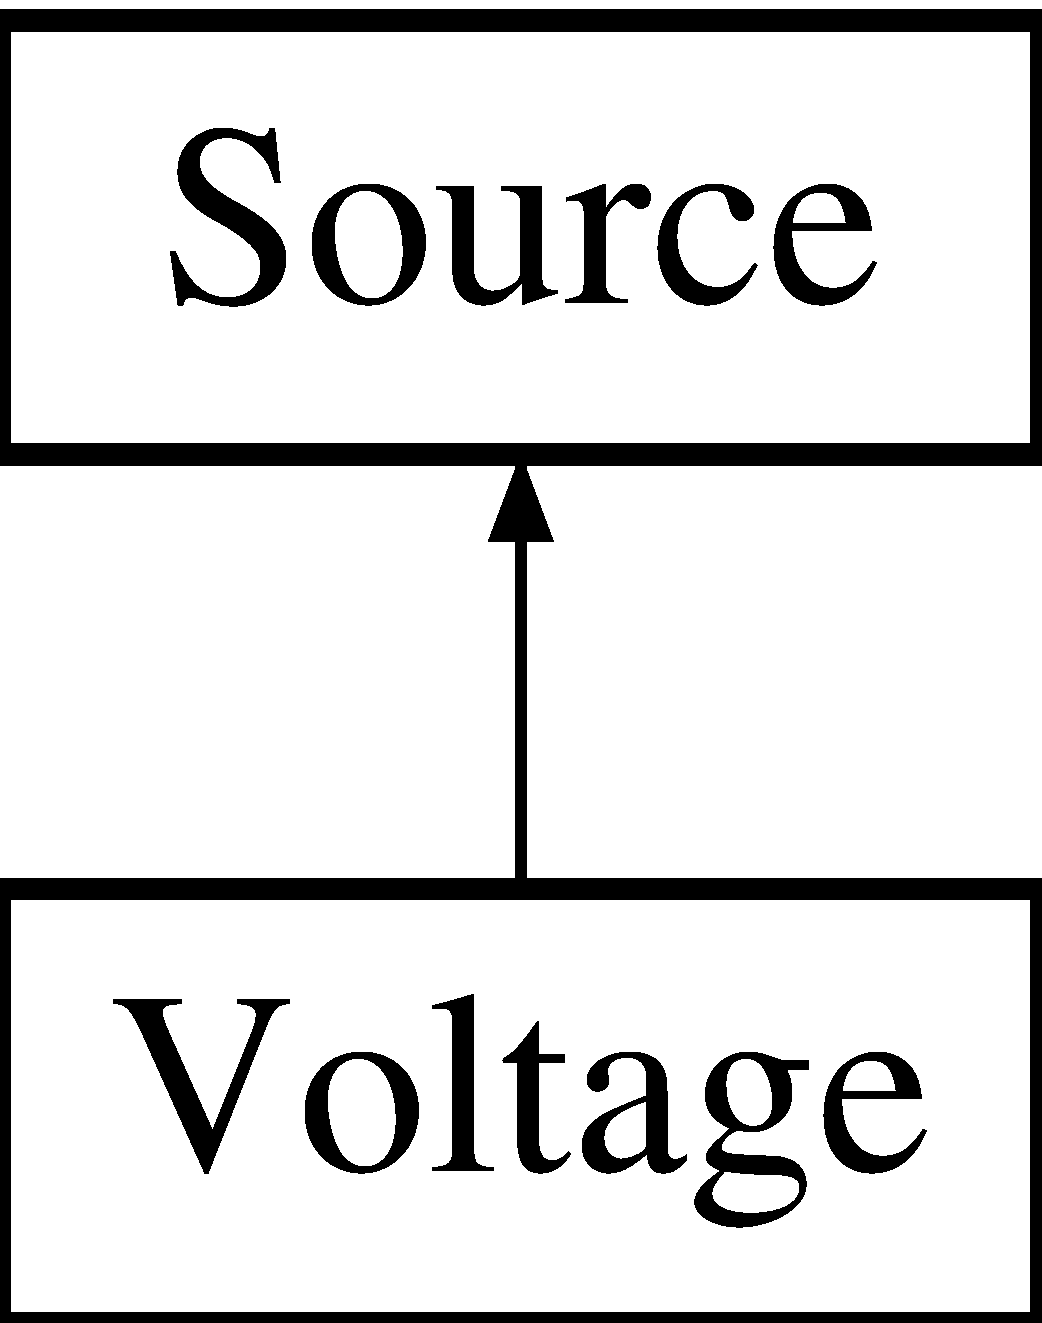
\includegraphics[height=2.000000cm]{class_s_p_i_c_e_1_1_voltage}
\end{center}
\end{figure}
\subsection*{Public Member Functions}
\begin{DoxyCompactItemize}
\item 
\mbox{\hyperlink{class_s_p_i_c_e_1_1_voltage_ae88c0ca0c1c79404c71ed3f4851a933d}{Voltage}} (std\+::string name, std\+::string pos, std\+::string neg, std\+::string value)
\begin{DoxyCompactList}\small\item\em creates a new voltage source. \end{DoxyCompactList}\end{DoxyCompactItemize}
\subsection*{Additional Inherited Members}


\subsection{Detailed Description}
This class describes a voltage source. 

\subsection{Constructor \& Destructor Documentation}
\mbox{\Hypertarget{class_s_p_i_c_e_1_1_voltage_ae88c0ca0c1c79404c71ed3f4851a933d}\label{class_s_p_i_c_e_1_1_voltage_ae88c0ca0c1c79404c71ed3f4851a933d}} 
\index{S\+P\+I\+C\+E\+::\+Voltage@{S\+P\+I\+C\+E\+::\+Voltage}!Voltage@{Voltage}}
\index{Voltage@{Voltage}!S\+P\+I\+C\+E\+::\+Voltage@{S\+P\+I\+C\+E\+::\+Voltage}}
\subsubsection{\texorpdfstring{Voltage()}{Voltage()}}
{\footnotesize\ttfamily \mbox{\hyperlink{class_s_p_i_c_e_1_1_voltage}{Voltage}} (\begin{DoxyParamCaption}\item[{std\+::string}]{name,  }\item[{std\+::string}]{pos,  }\item[{std\+::string}]{neg,  }\item[{std\+::string}]{value }\end{DoxyParamCaption})\hspace{0.3cm}{\ttfamily [inline]}}



creates a new voltage source. 


\begin{DoxyParams}{Parameters}
{\em name} & the name of the source. \\
\hline
{\em pos} & the positive connector of the source. \\
\hline
{\em neg} & the negative connector of the source. \\
\hline
{\em value} & the value of the source. \\
\hline
\end{DoxyParams}

\hypertarget{class_open_chams_1_1_v_slicing_node}{}\section{V\+Slicing\+Node Class Reference}
\label{class_open_chams_1_1_v_slicing_node}\index{V\+Slicing\+Node@{V\+Slicing\+Node}}
Inheritance diagram for V\+Slicing\+Node\+:\begin{figure}[H]
\begin{center}
\leavevmode
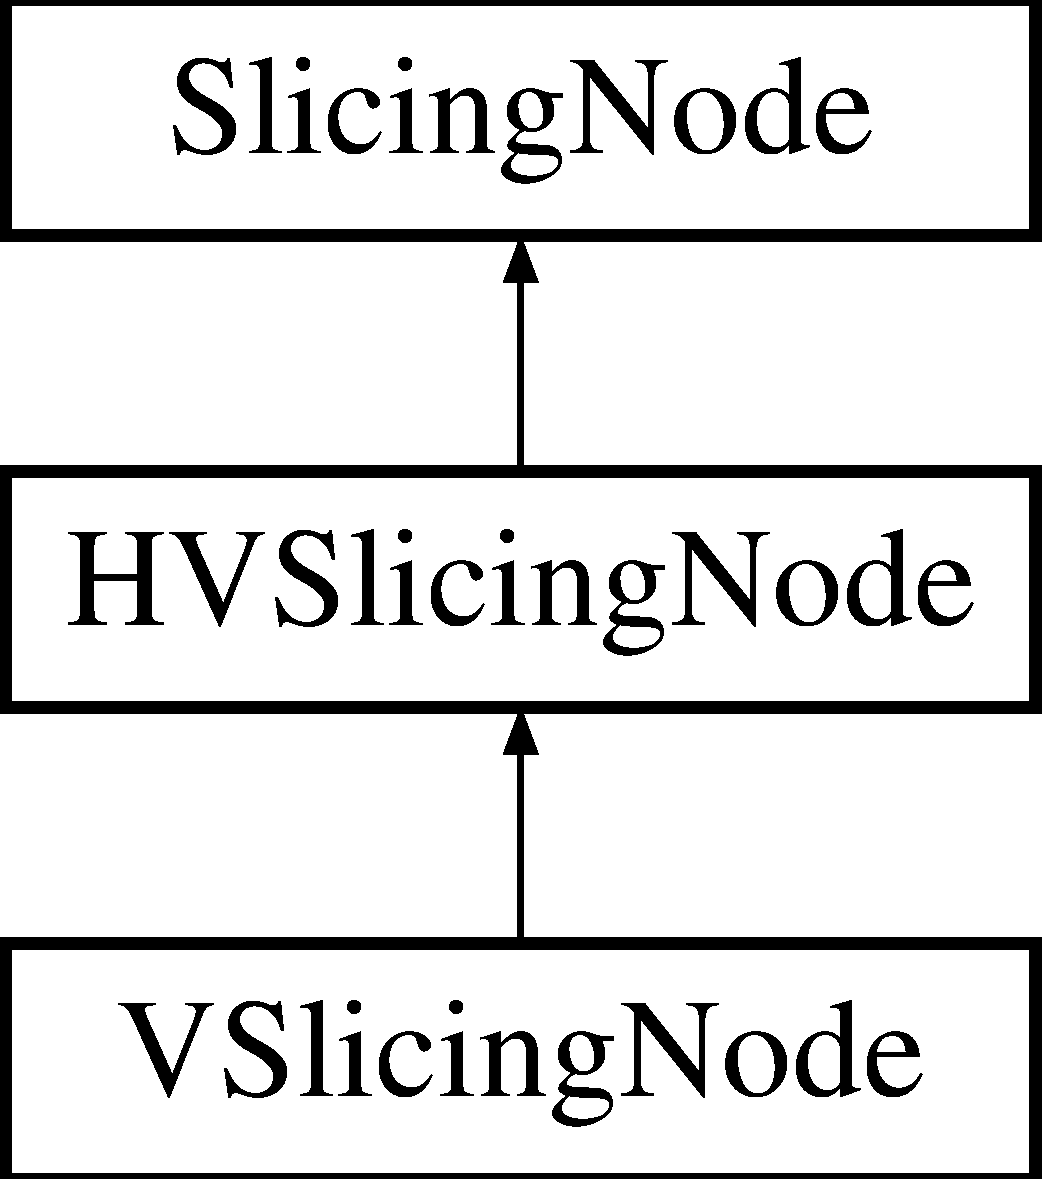
\includegraphics[height=3.000000cm]{class_open_chams_1_1_v_slicing_node}
\end{center}
\end{figure}

\hypertarget{class_open_chams_1_1_wire}{}\section{Wire Class Reference}
\label{class_open_chams_1_1_wire}\index{Wire@{Wire}}
\subsection*{Public Member Functions}
\begin{DoxyCompactItemize}
\item 
void \mbox{\hyperlink{class_open_chams_1_1_wire_aab66049b1f5ccf8de85249720152833a}{add\+Intermediate\+Point}} (double x, double y)
\begin{DoxyCompactList}\small\item\em adds an \mbox{\hyperlink{class_open_chams_1_1_intermediate_point}{Intermediate\+Point}} to the wire. \end{DoxyCompactList}\item 
\mbox{\Hypertarget{class_open_chams_1_1_wire_ab1c91025a4117cede119f53d9eb8093b}\label{class_open_chams_1_1_wire_ab1c91025a4117cede119f53d9eb8093b}} 
\mbox{\hyperlink{class_open_chams_1_1_wire_point}{Wire\+Point}} $\ast$ \mbox{\hyperlink{class_open_chams_1_1_wire_ab1c91025a4117cede119f53d9eb8093b}{get\+End\+Point}} ()
\begin{DoxyCompactList}\small\item\em returns the end point of the wire. \end{DoxyCompactList}\item 
\mbox{\Hypertarget{class_open_chams_1_1_wire_aac2840e22e03db0ff2c0fe0f83c56fdd}\label{class_open_chams_1_1_wire_aac2840e22e03db0ff2c0fe0f83c56fdd}} 
const std\+::vector$<$ \mbox{\hyperlink{class_open_chams_1_1_intermediate_point}{Intermediate\+Point}} $\ast$ $>$ \& \mbox{\hyperlink{class_open_chams_1_1_wire_aac2840e22e03db0ff2c0fe0f83c56fdd}{get\+Intermediate\+Points}} ()
\begin{DoxyCompactList}\small\item\em returns the list of wire\textquotesingle{}s \mbox{\hyperlink{class_open_chams_1_1_intermediate_point}{Intermediate\+Point}}. \end{DoxyCompactList}\item 
\mbox{\Hypertarget{class_open_chams_1_1_wire_ad68ddfcb6d4cbbe3c06d03fb4350dcdb}\label{class_open_chams_1_1_wire_ad68ddfcb6d4cbbe3c06d03fb4350dcdb}} 
\mbox{\hyperlink{class_open_chams_1_1_wire_point}{Wire\+Point}} $\ast$ \mbox{\hyperlink{class_open_chams_1_1_wire_ad68ddfcb6d4cbbe3c06d03fb4350dcdb}{get\+Start\+Point}} ()
\begin{DoxyCompactList}\small\item\em returns the start point of the wire. \end{DoxyCompactList}\item 
\mbox{\Hypertarget{class_open_chams_1_1_wire_abe5aa44c424e8b7bee9645af10ee0a23}\label{class_open_chams_1_1_wire_abe5aa44c424e8b7bee9645af10ee0a23}} 
bool \mbox{\hyperlink{class_open_chams_1_1_wire_abe5aa44c424e8b7bee9645af10ee0a23}{has\+No\+Intermediate\+Points}} ()
\begin{DoxyCompactList}\small\item\em returns true if the wire has no \mbox{\hyperlink{class_open_chams_1_1_intermediate_point}{Intermediate\+Point}}. \end{DoxyCompactList}\item 
void \mbox{\hyperlink{class_open_chams_1_1_wire_a25430c9acf02567164074625ba56e5ef}{set\+End\+Point}} (unsigned idx)
\begin{DoxyCompactList}\small\item\em sets the wire\textquotesingle{}s end point as a \mbox{\hyperlink{class_open_chams_1_1_port_point}{Port\+Point}}. \end{DoxyCompactList}\item 
void \mbox{\hyperlink{class_open_chams_1_1_wire_a37335a2ff923eb45ff5d4f2f4e41b8b1}{set\+Start\+Point}} (unsigned idx)
\begin{DoxyCompactList}\small\item\em sets the wire\textquotesingle{}s start point as a \mbox{\hyperlink{class_open_chams_1_1_port_point}{Port\+Point}}. \end{DoxyCompactList}\item 
\mbox{\Hypertarget{class_open_chams_1_1_wire_a66b8cdcb08d46fe66f1b910ff05ea328}\label{class_open_chams_1_1_wire_a66b8cdcb08d46fe66f1b910ff05ea328}} 
\mbox{\hyperlink{class_open_chams_1_1_wire_a66b8cdcb08d46fe66f1b910ff05ea328}{Wire}} ()
\begin{DoxyCompactList}\small\item\em creates a new wire. \end{DoxyCompactList}\end{DoxyCompactItemize}


\subsection{Detailed Description}
This class describes wire.

A wire is used by schematic to the connections between instances. It is defined by\+:
\begin{DoxyItemize}
\item a start point (\mbox{\hyperlink{class_open_chams_1_1_instance_point}{Instance\+Point}} or \mbox{\hyperlink{class_open_chams_1_1_port_point}{Port\+Point}}),
\item a end point (\mbox{\hyperlink{class_open_chams_1_1_instance_point}{Instance\+Point}} or \mbox{\hyperlink{class_open_chams_1_1_port_point}{Port\+Point}}),
\item a list of \mbox{\hyperlink{class_open_chams_1_1_intermediate_point}{Intermediate\+Point}}, this list may be empty.
\end{DoxyItemize}

\begin{DoxyNote}{Note}
Althought the \mbox{\hyperlink{class_open_chams_1_1_wire}{Wire}} object is related to \mbox{\hyperlink{class_open_chams_1_1_schematic}{Schematic}}, it is handled by \mbox{\hyperlink{class_open_chams_1_1_net}{Net}} object since a wire is always associated to a \mbox{\hyperlink{class_open_chams_1_1_net}{Net}}. 
\end{DoxyNote}


\subsection{Member Function Documentation}
\mbox{\Hypertarget{class_open_chams_1_1_wire_aab66049b1f5ccf8de85249720152833a}\label{class_open_chams_1_1_wire_aab66049b1f5ccf8de85249720152833a}} 
\index{Open\+Chams\+::\+Wire@{Open\+Chams\+::\+Wire}!add\+Intermediate\+Point@{add\+Intermediate\+Point}}
\index{add\+Intermediate\+Point@{add\+Intermediate\+Point}!Open\+Chams\+::\+Wire@{Open\+Chams\+::\+Wire}}
\subsubsection{\texorpdfstring{add\+Intermediate\+Point()}{addIntermediatePoint()}}
{\footnotesize\ttfamily void add\+Intermediate\+Point (\begin{DoxyParamCaption}\item[{double}]{x,  }\item[{double}]{y }\end{DoxyParamCaption})}



adds an \mbox{\hyperlink{class_open_chams_1_1_intermediate_point}{Intermediate\+Point}} to the wire. 


\begin{DoxyParams}{Parameters}
{\em x} & the x coordinate of the \mbox{\hyperlink{class_open_chams_1_1_intermediate_point}{Intermediate\+Point}}. \\
\hline
{\em y} & the y coordinate of the \mbox{\hyperlink{class_open_chams_1_1_intermediate_point}{Intermediate\+Point}}. \\
\hline
\end{DoxyParams}
\mbox{\Hypertarget{class_open_chams_1_1_wire_a25430c9acf02567164074625ba56e5ef}\label{class_open_chams_1_1_wire_a25430c9acf02567164074625ba56e5ef}} 
\index{Open\+Chams\+::\+Wire@{Open\+Chams\+::\+Wire}!set\+End\+Point@{set\+End\+Point}}
\index{set\+End\+Point@{set\+End\+Point}!Open\+Chams\+::\+Wire@{Open\+Chams\+::\+Wire}}
\subsubsection{\texorpdfstring{set\+End\+Point()}{setEndPoint()}}
{\footnotesize\ttfamily void set\+End\+Point (\begin{DoxyParamCaption}\item[{unsigned}]{idx }\end{DoxyParamCaption})}



sets the wire\textquotesingle{}s end point as a \mbox{\hyperlink{class_open_chams_1_1_port_point}{Port\+Point}}. 


\begin{DoxyParams}{Parameters}
{\em idx} & the index of the port associated to the \mbox{\hyperlink{class_open_chams_1_1_port_point}{Port\+Point}}. \\
\hline
\end{DoxyParams}
\mbox{\Hypertarget{class_open_chams_1_1_wire_a37335a2ff923eb45ff5d4f2f4e41b8b1}\label{class_open_chams_1_1_wire_a37335a2ff923eb45ff5d4f2f4e41b8b1}} 
\index{Open\+Chams\+::\+Wire@{Open\+Chams\+::\+Wire}!set\+Start\+Point@{set\+Start\+Point}}
\index{set\+Start\+Point@{set\+Start\+Point}!Open\+Chams\+::\+Wire@{Open\+Chams\+::\+Wire}}
\subsubsection{\texorpdfstring{set\+Start\+Point()}{setStartPoint()}}
{\footnotesize\ttfamily void set\+Start\+Point (\begin{DoxyParamCaption}\item[{unsigned}]{idx }\end{DoxyParamCaption})}



sets the wire\textquotesingle{}s start point as a \mbox{\hyperlink{class_open_chams_1_1_port_point}{Port\+Point}}. 


\begin{DoxyParams}{Parameters}
{\em idx} & the index of the port associated to the \mbox{\hyperlink{class_open_chams_1_1_port_point}{Port\+Point}}. \\
\hline
\end{DoxyParams}

\hypertarget{class_open_chams_1_1_wire_point}{\section{Wire\-Point Class Reference}
\label{class_open_chams_1_1_wire_point}\index{Wire\-Point@{Wire\-Point}}
}
Inheritance diagram for Wire\-Point\-:\begin{figure}[H]
\begin{center}
\leavevmode
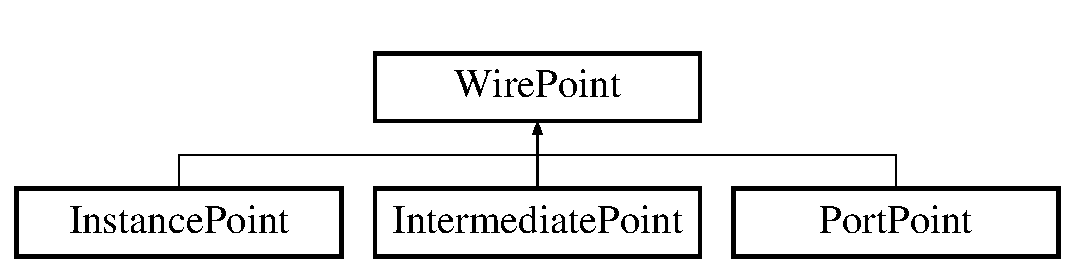
\includegraphics[height=2.000000cm]{class_open_chams_1_1_wire_point}
\end{center}
\end{figure}


\subsection{Detailed Description}
This class describes wire point. A wire point is an abstract object used to define all \char`\"{}direction changing\char`\"{} points of a wire. 
%--- End generated contents ---

% Index
\newpage
\phantomsection
\addcontentsline{toc}{part}{Index}
\printindex

\end{document}
